% Options for packages loaded elsewhere
%DIF LATEXDIFF DIFFERENCE FILE
%DIF DEL paper_R1.tex   Fri May 16 16:21:36 2025
%DIF ADD paper_R2.tex   Mon Jun 16 14:45:01 2025
\PassOptionsToPackage{unicode}{hyperref}
\PassOptionsToPackage{hyphens}{url}
%
\documentclass[
]{article}
\usepackage{amsmath,amssymb}
\usepackage{lmodern}
\usepackage{iftex}
\ifPDFTeX
  \usepackage[T1]{fontenc}
  \usepackage[utf8]{inputenc}
  \usepackage{textcomp} % provide euro and other symbols
\else % if luatex or xetex
  \usepackage{unicode-math}
  \defaultfontfeatures{Scale=MatchLowercase}
  \defaultfontfeatures[\rmfamily]{Ligatures=TeX,Scale=1}
\fi
% Use upquote if available, for straight quotes in verbatim environments
\IfFileExists{upquote.sty}{\usepackage{upquote}}{}
\IfFileExists{microtype.sty}{% use microtype if available
  \usepackage[]{microtype}
  \UseMicrotypeSet[protrusion]{basicmath} % disable protrusion for tt fonts
}{}
\makeatletter
\@ifundefined{KOMAClassName}{% if non-KOMA class
  \IfFileExists{parskip.sty}{%
    \usepackage{parskip}
  }{% else
    \setlength{\parindent}{0pt}
    \setlength{\parskip}{6pt plus 2pt minus 1pt}}
}{% if KOMA class
  \KOMAoptions{parskip=half}}
\makeatother
\usepackage{xcolor}
\IfFileExists{xurl.sty}{\usepackage{xurl}}{} % add URL line breaks if available
\IfFileExists{bookmark.sty}{\usepackage{bookmark}}{\usepackage{hyperref}}
\hypersetup{
  pdftitle={Space for WHAM: a multi-region, multi-stock generalization of the Woods Hole Assessment Model with an application to black sea bass},
  pdfauthor={Timothy J. Miller1; Kiersten L. Curti; Alexander C. Hansell},
  hidelinks,
  pdfcreator={LaTeX via pandoc}}
\urlstyle{same} % disable monospaced font for URLs
\usepackage[margin=1in]{geometry}
\usepackage{longtable,booktabs,array}
\usepackage{calc} % for calculating minipage widths
% Correct order of tables after \paragraph or \subparagraph
\usepackage{etoolbox}
\makeatletter
\patchcmd\longtable{\par}{\if@noskipsec\mbox{}\fi\par}{}{}
\makeatother
% Allow footnotes in longtable head/foot
\IfFileExists{footnotehyper.sty}{\usepackage{footnotehyper}}{\usepackage{footnote}}
\makesavenoteenv{longtable}
\usepackage{graphicx}
\makeatletter
\def\maxwidth{\ifdim\Gin@nat@width>\linewidth\linewidth\else\Gin@nat@width\fi}
\def\maxheight{\ifdim\Gin@nat@height>\textheight\textheight\else\Gin@nat@height\fi}
\makeatother
% Scale images if necessary, so that they will not overflow the page
% margins by default, and it is still possible to overwrite the defaults
% using explicit options in \includegraphics[width, height, ...]{}
\setkeys{Gin}{width=\maxwidth,height=\maxheight,keepaspectratio}
% Set default figure placement to htbp
\makeatletter
\def\fps@figure{htbp}
\makeatother
\setlength{\emergencystretch}{3em} % prevent overfull lines
\providecommand{\tightlist}{%
  \setlength{\itemsep}{0pt}\setlength{\parskip}{0pt}}
\setcounter{secnumdepth}{5}
\newlength{\cslhangindent}
\setlength{\cslhangindent}{1.5em}
\newlength{\csllabelwidth}
\setlength{\csllabelwidth}{3em}
\newlength{\cslentryspacingunit} % times entry-spacing
\setlength{\cslentryspacingunit}{\parskip}
\newenvironment{CSLReferences}[2] % #1 hanging-ident, #2 entry spacing
 {% don't indent paragraphs
  \setlength{\parindent}{0pt}
  % turn on hanging indent if param 1 is 1
  \ifodd #1
  \let\oldpar\par
  \def\par{\hangindent=\cslhangindent\oldpar}
  \fi
  % set entry spacing
  \setlength{\parskip}{#2\cslentryspacingunit}
 }%
 {}
\usepackage{calc}
\newcommand{\CSLBlock}[1]{#1\hfill\break}
\newcommand{\CSLLeftMargin}[1]{\parbox[t]{\csllabelwidth}{#1}}
\newcommand{\CSLRightInline}[1]{\parbox[t]{\linewidth - \csllabelwidth}{#1}\break}
\newcommand{\CSLIndent}[1]{\hspace{\cslhangindent}#1}
\usepackage{url}
\usepackage{setspace}
%\singlespacing
%\onehalfspacing
\doublespacing
\usepackage{lineno}
\linenumbers
\usepackage[belowskip=0pt,aboveskip=0pt]{caption}
\usepackage{relsize}
\usepackage{float}
% \usepackage[section]{placeins}
\usepackage{lscape}
\usepackage{longtable}
\usepackage{amsmath,rotating}
\usepackage[scanall]{psfrag}
\usepackage{bm}
\usepackage{caption,graphics}
\usepackage{graphicx}
%\usepackage{natbib}
%\usepackage[nottoc]{tocbibind}
%\usepackage{indentfirst}
\usepackage{sectsty}
\usepackage{color}
\usepackage{fancyhdr}
\usepackage{xspace}
\usepackage{textcomp}
\usepackage{upgreek}

\newcommand{\blandscape}{\begin{landscape}}
\newcommand{\elandscape}{\end{landscape}}
\newcommand{\noop}[1]{}
\usepackage{booktabs}
\usepackage{longtable}
\usepackage{array}
\usepackage{multirow}
\usepackage{wrapfig}
\usepackage{float}
\usepackage{colortbl}
\usepackage{pdflscape}
\usepackage{tabu}
\usepackage{threeparttable}
\usepackage{threeparttablex}
\usepackage[normalem]{ulem}
\usepackage{makecell}
\usepackage{xcolor}
\ifLuaTeX
  \usepackage{selnolig}  % disable illegal ligatures
\fi

\title{Space for WHAM: a multi-region, multi-stock generalization of the Woods Hole Assessment Model with an application to black sea bass}
\author{Timothy J. Miller\textsuperscript{1} \and Kiersten L. Curti \and Alexander C. Hansell}
\date{16 \DIFdelbegin \DIFdel{May}\DIFdelend \DIFaddbegin \DIFadd{June}\DIFaddend , 2025}
%DIF PREAMBLE EXTENSION ADDED BY LATEXDIFF
%DIF UNDERLINE PREAMBLE %DIF PREAMBLE
\RequirePackage[normalem]{ulem} %DIF PREAMBLE
\RequirePackage{color}\definecolor{RED}{rgb}{1,0,0}\definecolor{BLUE}{rgb}{0,0,1} %DIF PREAMBLE
\providecommand{\DIFaddtex}[1]{{\protect\color{blue}\uwave{#1}}} %DIF PREAMBLE
\providecommand{\DIFdeltex}[1]{{\protect\color{red}\sout{#1}}} %DIF PREAMBLE
%DIF SAFE PREAMBLE %DIF PREAMBLE
\providecommand{\DIFaddbegin}{} %DIF PREAMBLE
\providecommand{\DIFaddend}{} %DIF PREAMBLE
\providecommand{\DIFdelbegin}{} %DIF PREAMBLE
\providecommand{\DIFdelend}{} %DIF PREAMBLE
\providecommand{\DIFmodbegin}{} %DIF PREAMBLE
\providecommand{\DIFmodend}{} %DIF PREAMBLE
%DIF FLOATSAFE PREAMBLE %DIF PREAMBLE
\providecommand{\DIFaddFL}[1]{\DIFadd{#1}} %DIF PREAMBLE
\providecommand{\DIFdelFL}[1]{\DIFdel{#1}} %DIF PREAMBLE
\providecommand{\DIFaddbeginFL}{} %DIF PREAMBLE
\providecommand{\DIFaddendFL}{} %DIF PREAMBLE
\providecommand{\DIFdelbeginFL}{} %DIF PREAMBLE
\providecommand{\DIFdelendFL}{} %DIF PREAMBLE
%DIF HYPERREF PREAMBLE %DIF PREAMBLE
\providecommand{\DIFadd}[1]{\texorpdfstring{\DIFaddtex{#1}}{#1}} %DIF PREAMBLE
\providecommand{\DIFdel}[1]{\texorpdfstring{\DIFdeltex{#1}}{}} %DIF PREAMBLE
\newcommand{\DIFscaledelfig}{0.5}
%DIF HIGHLIGHTGRAPHICS PREAMBLE %DIF PREAMBLE
\RequirePackage{settobox} %DIF PREAMBLE
\RequirePackage{letltxmacro} %DIF PREAMBLE
\newsavebox{\DIFdelgraphicsbox} %DIF PREAMBLE
\newlength{\DIFdelgraphicswidth} %DIF PREAMBLE
\newlength{\DIFdelgraphicsheight} %DIF PREAMBLE
% store original definition of \includegraphics %DIF PREAMBLE
\LetLtxMacro{\DIFOincludegraphics}{\includegraphics} %DIF PREAMBLE
\newcommand{\DIFaddincludegraphics}[2][]{{\color{blue}\fbox{\DIFOincludegraphics[#1]{#2}}}} %DIF PREAMBLE
\newcommand{\DIFdelincludegraphics}[2][]{% %DIF PREAMBLE
\sbox{\DIFdelgraphicsbox}{\DIFOincludegraphics[#1]{#2}}% %DIF PREAMBLE
\settoboxwidth{\DIFdelgraphicswidth}{\DIFdelgraphicsbox} %DIF PREAMBLE
\settoboxtotalheight{\DIFdelgraphicsheight}{\DIFdelgraphicsbox} %DIF PREAMBLE
\scalebox{\DIFscaledelfig}{% %DIF PREAMBLE
\parbox[b]{\DIFdelgraphicswidth}{\usebox{\DIFdelgraphicsbox}\\[-\baselineskip] \rule{\DIFdelgraphicswidth}{0em}}\llap{\resizebox{\DIFdelgraphicswidth}{\DIFdelgraphicsheight}{% %DIF PREAMBLE
\setlength{\unitlength}{\DIFdelgraphicswidth}% %DIF PREAMBLE
\begin{picture}(1,1)% %DIF PREAMBLE
\thicklines\linethickness{2pt} %DIF PREAMBLE
{\color[rgb]{1,0,0}\put(0,0){\framebox(1,1){}}}% %DIF PREAMBLE
{\color[rgb]{1,0,0}\put(0,0){\line( 1,1){1}}}% %DIF PREAMBLE
{\color[rgb]{1,0,0}\put(0,1){\line(1,-1){1}}}% %DIF PREAMBLE
\end{picture}% %DIF PREAMBLE
}\hspace*{3pt}}} %DIF PREAMBLE
} %DIF PREAMBLE
\LetLtxMacro{\DIFOaddbegin}{\DIFaddbegin} %DIF PREAMBLE
\LetLtxMacro{\DIFOaddend}{\DIFaddend} %DIF PREAMBLE
\LetLtxMacro{\DIFOdelbegin}{\DIFdelbegin} %DIF PREAMBLE
\LetLtxMacro{\DIFOdelend}{\DIFdelend} %DIF PREAMBLE
\DeclareRobustCommand{\DIFaddbegin}{\DIFOaddbegin \let\includegraphics\DIFaddincludegraphics} %DIF PREAMBLE
\DeclareRobustCommand{\DIFaddend}{\DIFOaddend \let\includegraphics\DIFOincludegraphics} %DIF PREAMBLE
\DeclareRobustCommand{\DIFdelbegin}{\DIFOdelbegin \let\includegraphics\DIFdelincludegraphics} %DIF PREAMBLE
\DeclareRobustCommand{\DIFdelend}{\DIFOaddend \let\includegraphics\DIFOincludegraphics} %DIF PREAMBLE
\LetLtxMacro{\DIFOaddbeginFL}{\DIFaddbeginFL} %DIF PREAMBLE
\LetLtxMacro{\DIFOaddendFL}{\DIFaddendFL} %DIF PREAMBLE
\LetLtxMacro{\DIFOdelbeginFL}{\DIFdelbeginFL} %DIF PREAMBLE
\LetLtxMacro{\DIFOdelendFL}{\DIFdelendFL} %DIF PREAMBLE
\DeclareRobustCommand{\DIFaddbeginFL}{\DIFOaddbeginFL \let\includegraphics\DIFaddincludegraphics} %DIF PREAMBLE
\DeclareRobustCommand{\DIFaddendFL}{\DIFOaddendFL \let\includegraphics\DIFOincludegraphics} %DIF PREAMBLE
\DeclareRobustCommand{\DIFdelbeginFL}{\DIFOdelbeginFL \let\includegraphics\DIFdelincludegraphics} %DIF PREAMBLE
\DeclareRobustCommand{\DIFdelendFL}{\DIFOaddendFL \let\includegraphics\DIFOincludegraphics} %DIF PREAMBLE
%DIF AMSMATHULEM PREAMBLE %DIF PREAMBLE
\makeatletter %DIF PREAMBLE
\let\sout@orig\sout %DIF PREAMBLE
\renewcommand{\sout}[1]{\ifmmode\text{\sout@orig{\ensuremath{#1}}}\else\sout@orig{#1}\fi} %DIF PREAMBLE
\makeatother %DIF PREAMBLE
%DIF END PREAMBLE EXTENSION ADDED BY LATEXDIFF

\begin{document}
\maketitle

\(^1\)\href{mailto:timothy.j.miller@noaa.gov}{\nolinkurl{timothy.j.miller@noaa.gov}}, Northeast Fisheries Science Center, National Marine Fisheries Service, 166 Water Street, Woods Hole, MA 02543, USA\\

\pagebreak

\textbf{keywords:} stock assessment, state-space, multi-stock, multi-region, age-structured, black sea bass

\hypertarget{abstract}{%
\subsection*{Abstract}\label{abstract}}
\addcontentsline{toc}{subsection}{Abstract}

The Woods Hole Assessment Model is a general state-space age-structured assessment model that is used to assess and manage many stocks in the Northeast US. We first describe an extension of the model allowing any number of stocks (or stock components) and regions with movement among regions as well as seasonal variation in stock and fleet dynamics. Movement rates can be functions of time- and age-varying random effects and environmental covariates. We then illustrate the model by applying it to data for the northern and southern components of the Northeast United States black sea bass stock and evaluate alternative hypotheses of bottom temperature and time-varying random effects on recruitment and natural mortality. We show strong evidence for temperature effects on recruitment, primarily for the northern stock component, and no evidence for including random effects or temperature effects on age 1 natural mortality.

\pagebreak

\hypertarget{introduction}{%
\section*{Introduction}\label{introduction}}
\addcontentsline{toc}{section}{Introduction}

State-space age-structured stock assessment models can be used to estimate time and age-varying population attributes as random effects using maximum marginal likelihood or Bayesian fitting procedures (Nielsen and Berg 2014; Cadigan 2016; Miller et al. 2016b). This estimation approach is considered an essential feature of gold-standard assessment models that we use in tactical management of commercially important fish stocks (Punt et al. 2020). The State-space Assessment Model (SAM, Nielsen and Berg 2014) continues to be developed and remains widely used within the International Council for the Exploration of the Sea (ICES) to assess European fish stocks. Various state-space models are being used to manage cod and plaice stocks in the waters of Eastern Canada (Perreault et al. 2020; Varkey et al. 2022) and to the south, the Woods Hole Assessment Model (WHAM, \DIFdelbegin \DIFdel{Miller and Stock 2020; Stock }\DIFdelend \DIFaddbegin \DIFadd{Stock }\DIFaddend and Miller 2021) is now used to assess many fish stocks in the Northwest Atlantic Ocean (NEFSC 2022a, 2022b; NEFSC 2024a).

WHAM is an R package developed and maintained by scientists at NOAA's Northeast Fisheries Science Center (\url{https://timjmiller.github.io/wham}). WHAM can be configured to fit a wide range of age-structured models from traditional statistical catch-at-age models without any random effects\DIFaddbegin \DIFadd{, }\DIFaddend to models with several time and age varying process errors and effects of environmental covariates on various population parameters. Like SAM, WHAM models are built using the Template Model Builder package (TMB, Kristensen et al. 2016) which provides a computationally efficient means of fitting an extremely wide class of models with random effects. WHAM has undergone active development since its creation and includes random effects options for recruitment, inter-annual transitions of numbers at age (hereafter referred to as ``apparent survival''), fishery and index selectivity, natural mortality, and catchability.

However, WHAM has only allowed \DIFdelbegin \DIFdel{one stock and a single region and without }\DIFdelend \DIFaddbegin \DIFadd{consideration of a single stock and region, and no }\DIFaddend seasonal changes in stock dynamics. Using such models for stocks that have subcomponents with varying seasonal movement can provide incorrect inferences and poor management advice (Ying et al. 2011; Cao et al. 2014; Bosley et al. 2022). Furthermore, the ability to account for spatial structure and model multiple stocks are also important features of leading-edge assessment modeling frameworks (Punt et al. 2020). We describe here the implementation of these features and other extensions since Stock and Miller (2021) in WHAM version 2.0. Many of these new configuration options can also be useful when modeling a single stock and region.

We developed this extension of WHAM in concert with a research track assessment process for black sea bass (\DIFaddbegin \DIFadd{BSB, }\DIFaddend \textit{Centropristis striata}\DIFdelbegin \DIFdel{) (}\DIFdelend \DIFaddbegin \DIFadd{; }\DIFaddend NEFSC 2023)\DIFdelbegin \DIFdel{. Black sea bass }\DIFdelend \DIFaddbegin \DIFadd{, which }\DIFaddend is a high profile stock in the Northeast U.S. and important to both commercial fishing fleets and recreational anglers. \DIFdelbegin \DIFdel{Black sea bass }\DIFdelend \DIFaddbegin \DIFadd{BSB }\DIFaddend are targeted from Maine to North Carolina in both state and federal waters. Past stock assessments have estimated that the stock is healthy (not overfished and overfishing not occurring). \DIFdelbegin \DIFdel{Previous }\DIFdelend \DIFaddbegin \DIFadd{Those }\DIFaddend assessments assumed two stock components (north and south), each assessed with a separate statistical catch at age model\DIFaddbegin \DIFadd{, }\DIFaddend with results subsequently combined to inform management\DIFdelbegin \DIFdel{, but these assessments have }\DIFdelend \DIFaddbegin \DIFadd{. However, the assessments }\DIFaddend exhibited strong retrospective patterns. The stock was split into two regional components to account for spatial dynamics and improve model diagnostics (ASMFC 2016). Additionally, \DIFdelbegin \DIFdel{black sea bass }\DIFdelend \DIFaddbegin \DIFadd{BSB }\DIFaddend have complex spatial dynamics and make seasonal migrations, moving inshore in the spring and offshore in the fall (Moser and Shepherd 2009). \DIFdelbegin \DIFdel{Black sea bass }\DIFdelend \DIFaddbegin \DIFadd{BSB }\DIFaddend distribution has been linked to warming waters on the northwest shelf (Bell et al. 2015) and it is hypothesized that the distribution and productivity of the \DIFdelbegin \DIFdel{black sea bass }\DIFdelend \DIFaddbegin \DIFadd{BSB }\DIFaddend stock is especially susceptible to long-term changes in temperature causing increases in abundance further north (Hare et al. 2016). Thus, a focus of the \DIFdelbegin \DIFdel{black sea bass }\DIFdelend \DIFaddbegin \DIFadd{BSB }\DIFaddend research track assessment was to develop an assessment platform that could capture multiple stock components, complex seasonal movement, and explore environmental drivers of population dynamics (NEFSC 2023). We denote the fish in the north as separate stock components rather than stocks because both components are managed as a single stock, but recognizing differences in migration between fish originating in the two areas.

To illustrate the usage of WHAM 2.0 we apply it to the two stock components of \DIFdelbegin \DIFdel{black sea bass }\DIFdelend \DIFaddbegin \DIFadd{BSB }\DIFaddend off the coast of the Northeast United States (NEUS) using most of the model assumptions that were accepted during the peer-review process \DIFaddbegin \DIFadd{(NEFSC 2023)}\DIFaddend . However, here we evaluate evidence for alternative hypotheses of temporal variation and effects \DIFdelbegin \DIFdel{specifically }\DIFdelend of bottom temperature\DIFaddbegin \DIFadd{, specifically, }\DIFaddend on recruitment and natural mortality of age 1 individuals.

When modeling multiple stock components \DIFdelbegin \DIFdel{occurring in different }\DIFdelend \DIFaddbegin \DIFadd{and }\DIFaddend regions, further dimensionality is added to the class of possible equilbrium reference points (e.g., Kapur et al. 2021). Short term projections are also an important part of the management process and the separation of observation and process errors in state-space models allows uncertainty in projected attributes such as recruitment and spawning stock biomass (SSB) without external simulation exercises. Finally, the inclusion of explicit effects of environmental covariates in the model also requires assumptions on how they are treated in projections and reference points. We demonstrate some of the options of WHAM version 2.0 to provide biological reference points and short-term projections.

\hypertarget{methods}{%
\section*{Methods}\label{methods}}
\addcontentsline{toc}{section}{Methods}

\hypertarget{wham-description}{%
\subsection*{WHAM description}\label{wham-description}}
\addcontentsline{toc}{subsection}{WHAM description}

Many of the options and equations of WHAM version 2.0 are the same as those in Stock and Miller (2021), so we will only describe extensions and differences that have occurred since their first description of WHAM. The new version of WHAM can model multiple stocks\DIFaddbegin \DIFadd{, }\DIFaddend each with their own movement, harvest, and natural mortality. Much of the description below is for a specific stock \(s\), but, for simplicity, this subscript is implicit except when necessary.

\hypertarget{the-probability-transition-matrix}{%
\subsubsection*{The probability transition matrix}\label{the-probability-transition-matrix}}
\addcontentsline{toc}{subsubsection}{The probability transition matrix}

Because individuals may be alive in one of several regions or harvested \DIFdelbegin \DIFdel{in }\DIFdelend \DIFaddbegin \DIFadd{by }\DIFaddend one of several fleets, it is helpful to consider these as distinct categories or states and treat the number of individuals occurring in each category over time as a multi-state model. Approaches to modeling transitions among these states may treat time discretely (e.g., Arnason 1972; Schwarz et al. 1993) or continuously (e.g., Hearn et al. 1987; Commenges 1999; Andersen and Keiding 2002). We can define a probability transition matrix (PTM) that describes the probability of individuals occurring in different states at the end of a time interval with duration \(\delta\) (columns), conditional on being in each of those states at the beginning of the interval (rows). For fish populations, these states would be defined as being alive in a particular region or deceased due to fishing from a particular fleet or natural mortality. The time interval \(i\) with duration \(\delta_i\) would be a season and the PTMs would be uniquely defined for each stock by year \(y\), age \(a\), and season \(i\)\DIFdelbegin \DIFdel{on January 1. }\DIFdelend \DIFaddbegin \DIFadd{. }\DIFaddend Each row and column of the PTM correspond to one of the states: alive in region \(r\), dead in fleet \(f\), or dead from natural causes. The probabilities in each row sum to \DIFdelbegin \DIFdel{unity }\DIFdelend \DIFaddbegin \DIFadd{one }\DIFaddend (must be in one of the states) and assume an individual is in the state that corresponds to that row at the beginning of the interval. Given \(n_R\) regions and \(n_F\) fleets, the square PTM (\(n_R + n_F + 1\) rows and columns) as a function of sub-matrices is
\begin{equation}\label{eq:ptm}
  \mathbf{P}_{y,a,i} = \begin{bmatrix}
    \mathbf{O}_{y,a,i} & \mathbf{H}_{y,a,i} & \mathbf{D}_{y,a,i} \\
    0 & \mathbf{I}_{H} & 0\\
    0 & 0 & 1
  \end{bmatrix}\DIFaddbegin \DIFadd{,
}\DIFaddend \end{equation}
where
\begin{equation*}
  \mathbf{O}_{y,a,i} = 
  \begin{bmatrix}
    O_{y,a,i}(1,1) & \cdots & O_{y,a,i}(1,n_R) \\
    \vdots & \ddots & \vdots \\
    O_{y,a,i}(n_R,1) & \cdots & O_{y,a,i}(n_R,n_R)
  \end{bmatrix}
\end{equation*}
is the \(n_R \times n_R\) matrix defining survival and occurring in each region at the end of the interval,
\begin{equation*} 
  \mathbf{H}_{y,a,i} = 
  \begin{bmatrix}
    H_{y,a,i}(1,1) & \cdots & H_{y,a,i}(1,n_F) \\
    \vdots & \ddots & \vdots \\
    H_{y,a,i}(n_R,1) & \cdots & H_{y,a,i}(n_R,n_F)
  \end{bmatrix}
\end{equation*}
is the \(n_R \times n_F\) matrix defining probabilities of being captured in each fleet during the interval, and \(\mathbf{D}_{y,a,i}\) is the \DIFdelbegin \DIFdel{\(n_R x 1\) }\DIFdelend \DIFaddbegin \DIFadd{\(n_R \times 1\) }\DIFaddend matrix of probabilities of dying due to natural mortality during the interval. We have the \(n_F\times n_F\) identity matrix \(\mathbf{I}_{H}\) for the states of capture by each fleet and a 1 for the natural mortality state because the probabilities of being in one of the mortality states given starting the interval in that state is \DIFdelbegin \DIFdel{unity }\DIFdelend \DIFaddbegin \DIFadd{one }\DIFaddend (no zombies allowed).

WHAM uses these PTMs to model abundance proportions in each state rather than true probabilities where numbers in each state would have a multinomial distribution as in a model for tagging data where fates of individual tagged fish are assumed independent. The PTMs determine the expected numbers 1) in each state on January 1 of year \DIFdelbegin \DIFdel{\(t+1\) }\DIFdelend \DIFaddbegin \DIFadd{\(y+1\) }\DIFaddend at age \(a+1\) given the abundances at age \(a\) on January 1 of year \DIFdelbegin \DIFdel{\(t\)}\DIFdelend \DIFaddbegin \DIFadd{\(y\)}\DIFaddend , 2) captured over the year in each fleet, 3) available to each index, and 4) alive at the time and in the region where spawning occurs.

\hypertarget{single-region-ptms}{%
\subsubsection*{Single region PTMs}\label{single-region-ptms}}
\addcontentsline{toc}{subsubsection}{Single region PTMs}

When there is only one region,
\begin{equation}\label{eq:ptm_1_region}
\mathbf{P}_{y,a,i} = 
  \begin{bmatrix}
     S_{y,a,i} & \mathbf{H}_{y,a,i} & D_{y,a,i} \\
     0 & \mathbf{I}_{H} & 0\\
     0 & 0 & 1
  \end{bmatrix}\DIFaddbegin \DIFadd{,
}\DIFaddend \end{equation}
where \(S_{y,a,i} = e^{-Z_{y,a,i}\delta_i}\), \(\mathbf{H}_{y,a,i}\) is a 1 x \(n_F\) matrix with elements for each fleet \(f\): \DIFdelbegin \DIFdel{\(\frac{F_{y,a,i,f}}{Z_{y,a,i}}\left(1 - e^{-Z_{y,a,i}\delta_i}\right)\)}\DIFdelend \DIFaddbegin \DIFadd{\(\frac{F_{f,y,a,i}}{Z_{y,a,i}}\left(1 - e^{-Z_{y,a,i}\delta_i}\right)\)}\DIFaddend , \(D_{y,a,i} = \frac{M_{y,a}}{Z_{y,a,i}}\left(1 - e^{-Z_{y,a,i}\delta_i}\right)\), and \DIFdelbegin \DIFdel{\(Z_{y,a,i} = M_{y,a} + \sum^{n_F}_{f=1} F_{y,a,i,f}\) }\DIFdelend \DIFaddbegin \DIFadd{\(Z_{y,a,i} = M_{y,a} + \sum^{n_F}_{f=1} F_{f,y,a,i}\) }\DIFaddend is the total mortality rate.

\hypertarget{multi-region-ptms}{%
\subsubsection*{Multi-region PTMs}\label{multi-region-ptms}}
\addcontentsline{toc}{subsubsection}{Multi-region PTMs}

When there is more than one region, WHAM can model survival and movement as processes occurring sequentially or simultaneously. The sequential assumption is used widely in spatially explicit models (e.g., Stock Synthesis, Methot and Wetzel 2013). Under the sequential assumption, survival and death occur over the interval and movement among regions occurs instantly at either the beginning or the end of the interval. WHAM is configured to have movement occur after survival:
\begin{equation*}
  \mathbf{O}_{y,a,i} = \mathbf{S}_{y,a,i}\boldsymbol{\mu}_{y,a,i}\DIFaddbegin \DIFadd{,
}\DIFaddend \end{equation*}
where \(\mathbf{S}_{y,a,i}\) is a \(n_R \times n_R\) diagonal matrix of proportions surviving in each region (given they start in that region)
\begin{equation*}
\mathbf{S}_{y,a,i} = 
  \begin{bmatrix}
    e^{-Z_{y,a,i,1}\delta_i} & 0 & \cdots & 0 \\
    0 & e^{-Z_{y,a,i,2}\delta_i} & \cdots & 0 \\
    \vdots & \vdots & \ddots & \vdots \\
    0 & \cdots & 0 & e^{-Z_{y,a,i,n_R}\delta_i}
  \end{bmatrix}
\end{equation*}
and \(\boldsymbol{\mu}_{y,a,i}\) is a \(n_R \times n_R\) matrix of \DIFdelbegin \DIFdel{probabilities of }\DIFdelend \DIFaddbegin \DIFadd{proportions }\DIFaddend moving from one region to another or staying in the region they occurred at the beginning of the interval:
\begin{equation*}
\boldsymbol{\mu}_{y,a,i} = 
  \begin{bmatrix}
    1-\sum_{r' \neq 1} \mu_{1\rightarrow r',y,a,i} & \mu_{1\rightarrow 2,y,a,i} & \cdots & \mu_{1\rightarrow R,y,a,i} \\
    \mu_{2\rightarrow 1,y,a,i} & 1-\sum_{r' \neq 2} \mu_{2\rightarrow r',y,a,i} & \cdots & \mu_{2\rightarrow R,y,a,i} \\
    \vdots & \vdots & \ddots & \vdots \\
    \mu_{R\rightarrow 1,y,a,i} & \cdots & \mu_{R\rightarrow R-1,y,a,i} & 1-\sum_{r' \neq R} \mu_{R\rightarrow r',y,a,i}
  \end{bmatrix}
\end{equation*}

WHAM assumes each fleet \(f\) can harvest in only one region (\(r_f\)) during specified seasons. So, for each fleet \(f\), row \(r_f\) and column \(f\) of \(\mathbf{H}_{y,a,i}\) will be \DIFdelbegin \DIFdel{\(F_{y,a,i,f}\left(1 - e^{-Z_{y,a,i,r}\delta_i}\right)/Z_{y,a,i,r}\) }\DIFdelend \DIFaddbegin \DIFadd{\(F_{f,y,a,i}\left(1 - e^{-Z_{y,a,i,r}\delta_i}\right)/Z_{y,a,i,r}\) }\DIFaddend when fleet \(f\) is harvesting during the interval \(i\) and all other elements will be zero. Row \(r\) of the single-column matrix \(\mathbf{D}_{y,a,i}\) is \(M_{y,a,r}\left(1 - e^{-Z_{y,a,i,r}\delta_i}\right)/Z_{y,a,i,r}\). For details defining PTMs with movement and mortality \DIFdelbegin \DIFdel{occuring }\DIFdelend \DIFaddbegin \DIFadd{occurring }\DIFaddend simultaneously see Appendix B.

\hypertarget{seasonality}{%
\subsubsection*{Seasonality}\label{seasonality}}
\addcontentsline{toc}{subsubsection}{Seasonality}

Seasonality can be configured to accommodate characteristics of spawning, movement, and fleet-specific behavior. The annual time step can be divided into \(K\) seasons and the interval duration \(\delta_i\) for each season \(i\) does not need to be equal to any other seasonal interval. Under the Markov assumption the PTMs for each consecutive interval are independent and the PTM of surviving\DIFdelbegin \DIFdel{and moving}\DIFdelend \DIFaddbegin \DIFadd{, moving, }\DIFaddend and dying over \(K\) intervals \(1,\ldots, K\) (i.e., the entire year) is just the product of the PTMs for each interval:
\[ \mathbf{P}_{y,a}(\delta_1,\ldots,\delta_K) = \prod^K_{i=1}\mathbf{P}_{y,a,i}(\delta_i).\]

For a stock spawning at some fraction of the year \(0<t_s<1\) in interval \(i \in \{1,\ldots,K\}\), the fraction of time in the interval is
\[\delta_{s,i} = t_s-\sum^{i-1}_{j=0}\delta_j\]
(where \(\delta_0 = 0\))\DIFaddbegin \DIFadd{, }\DIFaddend and the PTM defining the proportions in each state at time \(t_s\) for age \(a\) is
\begin{equation}\label{eq:ptm_spawn}
\mathbf{P}_{y,a}\left(\delta_1,\ldots,\delta_{i-1}, \delta_{s,i}\right) = \mathbf{P}_{y,a}\left(t_s\right) =  \left[\prod^{i-1}_{j=0}\mathbf{P}_{y,a,j}(\delta_j)\right]\mathbf{P}_{y,a,i}(\delta_{s,i})\DIFaddbegin \DIFadd{,
}\DIFaddend \end{equation}
where \(\mathbf{P}_{y,a,0}\) is an identity matrix. Similarly, for an index \(m\) occurring at fraction of the year \(t_m\) in interval \(i\) the proportions in each state at the time of the observation is
\begin{equation} \label{eq:ptm_index} 
\mathbf{P}_{y,a}\left(\delta_1,\ldots,\delta_{i-1}, \delta_{m,i}\right) = \mathbf{P}_{y,a}\left(t_m\right) =   \left[\prod^{i-1}_{j=0}\mathbf{P}_{y,a,i}(\delta_j)\right]\mathbf{P}_{y,a,i}(\delta_{m,i}).
\end{equation}

\hypertarget{numbers-at-age}{%
\subsubsection*{Numbers at age}\label{numbers-at-age}}
\addcontentsline{toc}{subsubsection}{Numbers at age}

When there are \(n_R\) regions and \(n_F\) fleets, the vector of abundance \DIFaddbegin \DIFadd{for a given stock (component) }\DIFaddend in each state at age \(a>1\) on January 1 is \DIFdelbegin \DIFdel{\(\mathbf{N}_{y,a} = (\mathbf{N}_{O,y,a}^T, \mathbf{0}^T)^T\) }\DIFdelend \DIFaddbegin \DIFadd{\(\mathbf{N}_{y,a}^T = (\mathbf{N}_{O,y,a}^T, \mathbf{0}^T)\), }\DIFaddend where \(\mathbf{N}_{O,y,a} = (N_{y,a,1}, \ldots, N_{y,a,n_R})^T\) is the number in the states corresponding to being alive in each region and \(\mathbf{0}\) is a vector (\(n_F+1\)) for the numbers captured in each fleet \DIFdelbegin \DIFdel{and }\DIFdelend \DIFaddbegin \DIFadd{or }\DIFaddend dead from natural mortality because no age \(a\) fish have died yet on January 1.

Each stock \(s\) is assumed to spawn and recruit in one region \(r_s\). So for age \(a=1\), \(\mathbf{N}_{O,y,1}\) is 0 except for row \DIFdelbegin \DIFdel{\(r = r_s\)}\DIFdelend \DIFaddbegin \DIFadd{\(r_s\)}\DIFaddend . Options for configuring recruitment (\(N_{y,1,r_s}\)) for each stock are the same as previous versions of WHAM\DIFdelbegin \DIFdel{(Miller and Stock 2020)}\DIFdelend . If recruitment is assumed to be a function of SSB, it is only the spawning population in region \(r_s\) at the time of spawning that constitutes the SSB in the stock-recruit function. However, models can configure individuals to occur in other regions at the time of spawning. Aside from treating recruitment as a random walk, the general model for annual recruitment as random effects is
\begin{equation*}
\log\left(N_{y,1,r_s}\right)|\text{SSB}\DIFdelbegin \DIFdel{_{y-1,r_s} }\DIFdelend \DIFaddbegin \DIFadd{_{y-1} }\DIFaddend =  f\left(\text{SSB}\DIFdelbegin \DIFdel{_{y-1,r_s}}\DIFdelend \DIFaddbegin \DIFadd{_{y-1}}\DIFaddend \right) + \varepsilon_{y,1,r_s}\DIFaddbegin \DIFadd{,
}\DIFaddend \end{equation*}
where\\
\[\text{SSB}\DIFdelbegin \DIFdel{_{y,r_s} }\DIFdelend \DIFaddbegin \DIFadd{_{y} }\DIFaddend =  \sum^A_{a=1}  w_{y,a} \text{mat}_{y,a} \mathbf{O}\DIFdelbegin \DIFdel{_{y,a,r_s}}\DIFdelend \DIFaddbegin \DIFadd{_{y,a,\cdot,r_s}}\DIFaddend ^T(t_s) \mathbf{N}_{O,y,a}\]
and \(w_{y,a}\) and \(\text{mat}_{y,a}\) are the stock-specific mean weight at age of spawning individuals and maturity at age, respectively, and \DIFdelbegin \DIFdel{\(\mathbf{O}_{y,a,r_s}(t_s)\) }\DIFdelend \DIFaddbegin \DIFadd{\(\mathbf{O}_{y,a,\cdot,r_s}(t_s)\) }\DIFaddend are the probabilities of surviving and occurring in region \(r_s\) at time \(t_s\) given being alive in each region at the start of the year (\DIFdelbegin \DIFdel{the \(r_s\) column }\DIFdelend \DIFaddbegin \DIFadd{column \(r_s\) }\DIFaddend of the upper-left submatrix of Eq. \ref{eq:ptm_spawn}).

As in previous versions of WHAM, the apparent survival (and movement) from one year to another after recruitment can be treated deterministically or as functions of random effects. The predicted numbers at age \(a\) in year \(y\) for a given stock are vector analogs (\(\mathbf{N}_{O,y,a}\)) of the equations for numbers at age in the standard WHAM model (Stock and Miller 2021). For ages \(a = 2,\ldots, A-1\), where \(A\) is the plus group, the expected number alive in each region at the beginning of the following year and next age class age can be obtained from the first \(n_R\) elements of the vector
\[\mathbf{P}_{y-1,a-1}^T \mathbf{N}_{y-1,a-1}.\]
The numbers alive in each region can also be modeled more simply using the sub-matrix \(\mathbf{O}_{y,a}\). The general model for the vector of abundance at age in year \(y\) at age \(a\) given the vector in year \(y-1\) at age \(a-1\) is
\begin{equation*}
\log\left(\mathbf{N}_{O,y,a}\right)|\mathbf{N}_{O,y-1,a-1} =  \log\left(\mathbf{O}_{y-1,a-1}^T \mathbf{N}_{O,y-1,a-1}\right) + \boldsymbol{\varepsilon}_{y,a}
\end{equation*}
for ages \(a = 2,\ldots, A-1\), and for the plus group
\begin{equation*}
\log\left(\mathbf{N}_{O,y,A}\right)|\mathbf{N}_{O,y-1,A-1},\mathbf{N}_{O,y-1,A} = \log\left(\mathbf{O}_{y-1,A-1}^T \mathbf{N}_{O,y-1,A-1} + \mathbf{O}_{y-1,A}^T \mathbf{N}_{O,y-1,A}\right) + \boldsymbol{\varepsilon}_{y,A}\DIFaddbegin \DIFadd{,
}\DIFaddend \end{equation*}
where \(\boldsymbol{\varepsilon}_{y,a}\) is the vector of region-specific errors for a given stock, which are independent across stocks and regions, but the same correlation structures as previous versions are possible across ages and years for a given stock and region.

When there is autocorrelation with age, WHAM now assumes this applies only to ages \(a>1\) by default so that recruitment random effects are independent of those for the apparent survival of older age classes. \DIFdelbegin \DIFdel{So the }\DIFdelend \DIFaddbegin \DIFadd{The }\DIFaddend general covariance structure for a given stock at ages \(a>1\) in region \(r\) is \DIFdelbegin \DIFdel{that of }\DIFdelend a two-dimensional first-order autoregressive (2DAR1) process
\begin{equation*}
  Cov\left(\varepsilon_{y,a,r},\varepsilon_{y',a',r}\right) =   \frac{\rho_{N,\text{age},r}^{|a-a'|}\rho_{N,\text{year},r}^{|y-y'|}\sigma_{N,a,r}\sigma_{N,a',r}}{\left(1 -  \rho_{N,\text{age},r}^2\right)\left(1 - \rho_{N,\text{year},r}^2\right)} 
\end{equation*}
and that for age 1 is just AR1 across years
\begin{equation*}
  Cov\left(\varepsilon_{y,1},\varepsilon_{y',1}\right) =   \frac{\rho_{N,1,\text{year}}^{|y-y'|}\sigma^2_{N,1}}{1 - \rho_{N,1,\text{year}}^2}.
\end{equation*}
\DIFdelbegin \DIFdel{When }\DIFdelend \DIFaddbegin \DIFadd{If }\DIFaddend the annual changes in abundance at age are treated deterministically, \DIFdelbegin \DIFdel{\(\boldsymbol{\varepsilon}_{y,a} = 0\)}\DIFdelend \DIFaddbegin \DIFadd{then \(\boldsymbol{\varepsilon}_{y,a} = \mathbf{0}\)}\DIFaddend . Since recruitment for a given stock currently only occurs in one region \(r_s\) there is only a single vector of time-varying recruitment random effects for each stock.

\hypertarget{initial-numbers-at-age}{%
\subsubsection*{Initial numbers at age}\label{initial-numbers-at-age}}
\addcontentsline{toc}{subsubsection}{Initial numbers at age}

Initial numbers at age for each stock and region can be treated as age-specific fixed effects or with an equilibrium assumption as in previous versions of WHAM. For the equilibrium option there are two parameters for each stock: the stock-specific \DIFaddbegin \DIFadd{equilibrium }\DIFaddend fully-selected fishing mortality rate \DIFdelbegin \DIFdel{\(\log \widetilde{F}\) }\DIFdelend \DIFaddbegin \DIFadd{(\(\widetilde{F}_1\)) }\DIFaddend and the recruitment in year 1 \DIFdelbegin \DIFdel{\(\log N_{1,1,r_s}\)}\DIFdelend \DIFaddbegin \DIFadd{(\(N_{1,1,r_s}\))}\DIFaddend . A stock-specific equilibrium fishing mortality at age by fleet \DIFdelbegin \DIFdel{\({\tilde F}_{a,f}\) }\DIFdelend \DIFaddbegin \DIFadd{(\(\widetilde{F}_{f,1,a}\)) }\DIFaddend is the product of \DIFdelbegin \DIFdel{\(\widetilde{F}\) }\DIFdelend \DIFaddbegin \DIFadd{\(\widetilde{F}_1\) }\DIFaddend and the selectivity across fleets in the first year
\begin{equation*}
  \text{sel}\DIFdelbegin \DIFdel{_{1,a,f} }\DIFdelend \DIFaddbegin \DIFadd{_{f,1,a} }\DIFaddend = \DIFdelbegin \DIFdel{\frac{F_{1,a,f}}{\max_a \sum_{f=1}^{n_F} F_{1,a,f}}}\DIFdelend \DIFaddbegin \DIFadd{\frac{F_{f,1,a}}{\max_a \sum_{f=1}^{n_F} F_{f,1,a}}}\DIFaddend .
\end{equation*}
We use \DIFdelbegin \DIFdel{\(\widetilde{F}_{a,f}\) }\DIFdelend \DIFaddbegin \DIFadd{\(\widetilde{F}_{f,1,a}\) }\DIFaddend to define an equilibrium abundance per recruit by region at age \(a\) conditional on recruiting to each region
\begin{equation}\label{eq:npraa}
 \widetilde{\mathbf{O}}_{a} = \left\{
 \begin{array}{ll}
\prod^{a-1}_{j=0}\mathbf{O}_{j}  & 1\leq a<A\\
\left[\prod^{a-1}_{j=0}\mathbf{O}_{j}\right] \left(\mathbf{I} - \mathbf{O}_{A}\right)^{-1} & a = A
 \end{array}\DIFaddbegin \DIFadd{,
}\DIFaddend \right.
\end{equation}
where \(\mathbf{O}_{j}\) is the equilibrium \DIFdelbegin \DIFdel{probability of }\DIFdelend \DIFaddbegin \DIFadd{proportions }\DIFaddend surviving age \(a\) and occurring in each region and \(\mathbf{O}_{0} = \mathbf{I}\)\DIFaddbegin \DIFadd{, the identity matrix}\DIFaddend . Natural mortality and movement rates in the first year of the model are also used in Eq. \ref{eq:npraa}. For the plus group \(a=A\), \(\left(\mathbf{I} - \mathbf{O}_{A}\right)^{-1}\) is a ``fundamental matrix'\,' derived using the matrix version of the geometric series (Kemeny and Snell 1960). Recall that recruitment for \DIFaddbegin \DIFadd{a given }\DIFaddend stock \(s\) only occurs in region \(r_s\) so, the equilibrium initial numbers at age \(a\) by region are
\[\mathbf{N}_{O,1,a} = \widetilde{\mathbf{O}}\DIFdelbegin \DIFdel{_{a}^T \mathbf{N}_{O,1,1}.}\DIFdelend \DIFaddbegin \DIFadd{_{a,r_s,\cdot} N_{1,1,r_s},}\DIFaddend \]
\DIFaddbegin \DIFadd{where \(\widetilde{\mathbf{O}}_{a,r_s,\cdot}\) is the vector of values in row \(r_s\) of \(\widetilde{\mathbf{O}}_{a}\). }\DIFaddend Initial abundance at age can also be estimated as random effects as described in Appendix B.

\hypertarget{parametizing-movement}{%
\subsubsection*{Parametizing movement}\label{parametizing-movement}}
\addcontentsline{toc}{subsubsection}{Parametizing movement}

For each season, there are at most \(n_R-1\) parameters determining movement for a given stock among regions given starting the season in region \(r\) in either the sequential or simultaneous configurations. Movement parameters are estimated on a transformed scale via a link function \(g(\cdot)\). If survival and movement occur simultaneously, the parameters are estimated with a log link function and if they are separable, an additive logit link function (like a multinomial regression) is used. On the transformed scale, the general model for the movement parameter from region \(r\) to \(r'\) in season \(i\) and year \(y\) for individuals of age \(a\) is a linear function of an intercept or mean parameter (\(\theta_{r\rightarrow r',i}\)) and both random and \DIFdelbegin \DIFdel{environmental effects:
}\DIFdelend \DIFaddbegin \DIFadd{covariate effects:
}\DIFaddend \begin{equation*}
  g(\mu_{r\rightarrow r',y,a,i}) = \theta_{r\rightarrow r',i} + \varepsilon_{r\rightarrow r',y,a,i} + \sum^{n_E}_{k=1} \beta_{r \rightarrow r',a,i,k} \DIFdelbegin \DIFdel{E}\DIFdelend \DIFaddbegin \DIFadd{X}\DIFaddend _{k,y}.
\end{equation*}
The random effects \(\varepsilon_{r\rightarrow r',y,a,i}\) are \DIFdelbegin \DIFdel{season-, and region-to-region-specific }\DIFdelend \DIFaddbegin \DIFadd{region-to-region- }\DIFaddend and \DIFaddbegin \DIFadd{season-specific, and }\DIFaddend modeled most generally as 2DAR1 random effects with age and(or) year\DIFaddbegin \DIFadd{, }\DIFaddend where the covariance is
\begin{equation*}
  Cov\left(\varepsilon_{r\rightarrow r',y,a,i},\varepsilon_{r\rightarrow r',y',a',i}\right) =   \frac{\rho_{r\rightarrow r',\text{age},i}^{|a-a'|}\rho_{r\rightarrow r',\text{year},i}^{|y-y'|}\sigma^2_{r\rightarrow r',i}}{\left(1 -  \rho_{r\rightarrow r',\text{age},i}^2\right)\left(1 - \rho_{r\rightarrow r',\text{year},i}^2\right)}\DIFaddbegin \DIFadd{.
}\DIFaddend \end{equation*}
\DIFaddbegin \DIFadd{This is }\DIFaddend similar to how WHAM models variation in survival, natural mortality, and selectivity. \DIFdelbegin \DIFdel{Effects of covariate \(E_k\) can be }\DIFdelend \DIFaddbegin \DIFadd{Covariate \(X_k\) effects (\(\beta_{r\rightarrow r',a,i,k}\)) can be region-to-region-, }\DIFaddend age-, \DIFdelbegin \DIFdel{season-, and region-to-region-specific \(\beta_{r\rightarrow r',a,i,k}\) }\DIFdelend and \DIFaddbegin \DIFadd{season-specific, and }\DIFaddend the same orthogonal polynomial options in the previous versions of WHAM for effects on recruitment and natural mortality are available.

There is currently no likelihood component for tagging data. Therefore, movement parameters would usually either need to be fixed or assumed to have some prior distribution, possibly based on external parameter estimates. WHAM includes prior distributions for the \DIFdelbegin \DIFdel{season and region-to-region specific }\DIFdelend \DIFaddbegin \DIFadd{region-to-region- and season-specific }\DIFaddend (mean) movement parameters and treats them as random effects with the mean defined by the initial value of the fixed effect counterpart and standard deviation
\begin{equation*}
  \gamma_{r\rightarrow r',i} \sim \text{N}\left(\theta_{r\rightarrow r',i}, \sigma^2\DIFdelbegin \DIFdel{_{r\rightarrow r',i}}\DIFdelend \DIFaddbegin \DIFadd{_{\gamma,r\rightarrow r',i}}\DIFaddend \right).
  \end{equation*}
When priors are used, the movement is defined instead as
\begin{equation*}
  g(\mu_{r\rightarrow r',y,a,i}) = \gamma_{r\rightarrow r',i} + \varepsilon_{r\rightarrow r',y,a,i} + \sum^{n_E}_{k=1} \beta_{r\rightarrow r',a,i,k} \DIFdelbegin \DIFdel{E}\DIFdelend \DIFaddbegin \DIFadd{X}\DIFaddend _{k,y}.
  \end{equation*}

\hypertarget{natural-mortality}{%
\subsubsection*{Natural mortality}\label{natural-mortality}}
\addcontentsline{toc}{subsubsection}{Natural mortality}

When treated as constant parameters, natural mortality rates may be stock-, region-, and age-specific, but currently are constant across seasons. When random effects are used, the same 2DAR1 structure with age and year as described by Stock and Miller (2021) can be configured for a given stock and region and any environmental covariate effects can be stock-, region-, and age-specific. \DIFdelbegin \DIFdel{See Appendix Bfor details}\DIFdelend \DIFaddbegin \DIFadd{We provide details in Appendix B}\DIFaddend .

\hypertarget{catch-observations}{%
\subsubsection*{Catch observations}\label{catch-observations}}
\addcontentsline{toc}{subsubsection}{Catch observations}

The log-normal distributional assumption for aggregate catch observations is the same as Stock and Miller (2021), but the predicted catch is now a function of catch from each stock starting the year in each region and any seasonal movement. For a given stock \DIFdelbegin \DIFdel{and age }\DIFdelend \DIFaddbegin \DIFadd{\(s\) at age \(a\)}\DIFaddend , the vector of numbers captured by each fleet over the year \DIFdelbegin \DIFdel{are
}\DIFdelend \DIFaddbegin \DIFadd{\(y\) is
}\DIFaddend \[\DIFdelbegin %DIFDELCMD < \widehat{\mathbf{N}}%%%
\DIFdelend \DIFaddbegin \DIFadd{\mathbf{N}}\DIFaddend _{H,s,y,a} = \mathbf{H}_{s,y,a}^T \mathbf{N}_{O,s,y,a}\]
(recall each fleet can harvest in only one region as described above). The vector of \DIFdelbegin \DIFdel{predicted }\DIFdelend numbers caught by each fleet across stocks is
\[\DIFdelbegin %DIFDELCMD < \widehat{\mathbf{N}}%%%
\DIFdelend \DIFaddbegin \DIFadd{\mathbf{N}}\DIFaddend _{H,y,a} = \sum^{n_S}_{s=1} \DIFdelbegin %DIFDELCMD < \widehat{\mathbf{N}}%%%
\DIFdelend \DIFaddbegin \DIFadd{\mathbf{N}}\DIFaddend _{H,s,y,a}\]
and the vector of predicted aggregate catch by each fleet at age \(a\) is
\[\widehat{\mathbf{C}}_{y,a} = \text{diag}\left(\mathbf{c}_{y,a}\right) \DIFdelbegin %DIFDELCMD < \widehat{\mathbf{N}}%%%
\DIFdelend \DIFaddbegin \DIFadd{\mathbf{N}}\DIFaddend _{H,y,a}\DIFaddbegin \DIFadd{,}\DIFaddend \]
where \(\mathbf{c}_{y,a}\) is the vector of mean individual weight at age \(a\) for each fleet and the aggregate catch by fleet is
\[\widehat{\mathbf{C}}_y = \sum^{A}_{a=1} \widehat{\mathbf{C}}_{y,a}.\]
The log-aggregate catch observations for fleet \(f\) are normally distributed
\[ \log C\DIFdelbegin \DIFdel{_{y,f} }\DIFdelend \DIFaddbegin \DIFadd{_{f,y} }\DIFaddend \sim \text{N}\left(\log \widehat {C}\DIFdelbegin \DIFdel{_{y,f}}\DIFdelend \DIFaddbegin \DIFadd{_{f,y}}\DIFaddend , \sigma^2\DIFdelbegin \DIFdel{_{y,f}}\DIFdelend \DIFaddbegin \DIFadd{_{f,y}}\DIFaddend \right)\DIFdelbegin \DIFdel{.}\DIFdelend \DIFaddbegin \DIFadd{,}\DIFaddend \]

\DIFaddbegin \DIFadd{where \(\widehat C_{f,y}\) is an element of \(\widehat{\mathbf{C}}_y\). }\DIFaddend The predicted numbers caught for each fleet \(f\) (row \(f\) of \DIFdelbegin \DIFdel{\(\widehat{\mathbf{N}}_{H,y,a}\)}\DIFdelend \DIFaddbegin \DIFadd{\(\mathbf{N}_{H,y,a}\)}\DIFaddend ) are used to make predicted age composition observations as described by Stock and Miller (2021). Since then, three additional likelihood options for age composition observations have been added: a logistic-normal with AR(1) correlation structure (Francis 2014), the alternative Dirichlet-multinomial parameterization described by Thorson et al. (2017), and the multivariate Tweedie (Thorson et al. 2023).

\hypertarget{index-observations}{%
\subsubsection*{Index observations}\label{index-observations}}
\addcontentsline{toc}{subsubsection}{Index observations}

\DIFdelbegin \DIFdel{Like fishing fleets, an }\DIFdelend \DIFaddbegin \DIFadd{An }\DIFaddend index \(m\) can observe \DIFdelbegin \DIFdel{the population }\DIFdelend \DIFaddbegin \DIFadd{any stocks that occur }\DIFaddend in a single region \(r_m\) at fraction of the year \(t_m\)\DIFdelbegin \DIFdel{, the predicted }\DIFdelend \DIFaddbegin \DIFadd{. The }\DIFaddend abundance at \(t_m\) in region \(r_m\) is
\[\DIFdelbegin %DIFDELCMD < \widehat{N}%%%
\DIFdel{_{s,y,a,m} }\DIFdelend \DIFaddbegin \DIFadd{N_{m,s,y,a} }\DIFaddend = \mathbf{O}\DIFdelbegin \DIFdel{_{s,y,a,r_m}}\DIFdelend \DIFaddbegin \DIFadd{_{s,y,a,\cdot,r_m}}\DIFaddend ^T(t_m) \mathbf{N}_{O,s,y,a}\DIFaddbegin \DIFadd{,}\DIFaddend \]
where \DIFdelbegin \DIFdel{\(\mathbf{O}_{s,y,a,r_m}(t_m)\), the \(r_m\) column }\DIFdelend \DIFaddbegin \DIFadd{\(\mathbf{O}_{s,y,a,\cdot,r_m}(t_m)\), column \(r_m\) }\DIFaddend of the upper-left submatrix of Eq. \ref{eq:ptm_index}, \DIFdelbegin \DIFdel{are the probabilities of }\DIFdelend \DIFaddbegin \DIFadd{is the vector of proportions }\DIFaddend surviving and occurring in region \(r_m\) at time \(t_m\) given being alive in each region at the start of the year. The predicted index at age is
\[\widehat{I}_{m,y,a} = q_{m,y} \text{sel}_{m,y,a}w_{m,y,a}\sum^{n_S}_{s = 1}\DIFdelbegin %DIFDELCMD < \widehat{N}%%%
\DIFdel{_{s,y,a,m}}\DIFdelend \DIFaddbegin \DIFadd{N_{m,s,y,a},}\DIFaddend \]
where \(q_{m,y}\) is the catchability of the index in year \(y\), \(\text{sel}_{m,y,a}\) is the selectivity\DIFaddbegin \DIFadd{, }\DIFaddend and \(w_{m,y,a}\) is the average weight of individuals at age \(a\) if the index is quantified in biomass and \(w_{m,y,a} = 1\) if the index is quantified in numbers. Predicted age composition observations are functions of \(\widehat{I}_{m,y,a}\) as described by Stock and Miller (2021) and the likelihood options are the same as those for catch explained above. \DIFdelbegin \DIFdel{See Appendix B for }\DIFdelend \DIFaddbegin \DIFadd{We describe }\DIFaddend options to model temporal variation in catchability \DIFaddbegin \DIFadd{in Appendix B}\DIFaddend .

\hypertarget{reference-points}{%
\subsubsection*{Reference points}\label{reference-points}}
\addcontentsline{toc}{subsubsection}{Reference points}

\DIFdelbegin \DIFdel{Currently a }\DIFdelend \DIFaddbegin \DIFadd{WHAM calculates annual reference points using biological inputs each year and it also provides the same reference points under prevailing conditions where biological inputs are averaged over a user-defined set of recent years. A }\DIFaddend single fishing mortality reference point \DIFdelbegin \DIFdel{\(\widetilde F\) }\DIFdelend \DIFaddbegin \DIFadd{\(\widetilde{F}\) }\DIFaddend is estimated across stocks and regions and the fleet- and age-specific reference point is \DIFdelbegin \DIFdel{\(\widetilde F_{f,a} = \widetilde F \text{sel}_{f,a}\)}\DIFdelend \DIFaddbegin \DIFadd{\(\widetilde{F}_{f,a} = \widetilde{F} \text{sel}_{f,a}\)}\DIFaddend . Selectivity is determined across fleets and ages as in the equilibrium assumption for initial abundance at age except here it is a function of \DIFdelbegin \DIFdel{average F at ageover a user-defined set of years}\DIFdelend \DIFaddbegin \DIFadd{fishing mortality at age, possibly averaged over years,
}\DIFaddend \begin{equation}\label{eq:spr_sel}
  \text{sel}\DIFdelbegin \DIFdel{_{a,f} }\DIFdelend \DIFaddbegin \DIFadd{_{f,a} }\DIFaddend = \DIFdelbegin \DIFdel{\frac{\overline F_{a,f}}{\max_a \sum^{n_F}_{f=1}{\overline F}_{a,f}}
}\DIFdelend \DIFaddbegin \DIFadd{\frac{\overline{F}_{f,a}}{\max_a \sum^{n_F}_{f=1}{\overline{F}}_{f,a}}.
}\DIFaddend \end{equation}

The equilibrium spawning stock \DIFdelbegin \DIFdel{biomass per recruit }\DIFdelend \DIFaddbegin \DIFadd{biomass-per-recruit }\DIFaddend for a given stock in region \(r_s\) is defined as
\begin{equation}\label{eq:ssbpr}
 \upphi(\widetilde{F}) = \sum^{A}_{a=1} \widetilde{\mathbf{O}}_{a,r_s,\cdot} \mathbf{O}_{a,\cdot,r_s}(t_s) w_{a} m_{a}\DIFaddbegin \DIFadd{,
}\DIFaddend \end{equation}
where \(w_{a}\) and \(m_{a}\) are the mean individual weight and \DIFdelbegin \DIFdel{probability of maturity }\DIFdelend \DIFaddbegin \DIFadd{proportion mature }\DIFaddend at age \(a\), \DIFdelbegin \DIFdel{\(\widetilde{\mathbf{O}}_{a}\) are as described }\DIFdelend \DIFaddbegin \DIFadd{\(\widetilde{\mathbf{O}}_{a,r_s,\cdot}\) is row \(r_s\) of \(\widetilde{\mathbf{O}}_a\) }\DIFaddend in Eq. \ref{eq:npraa}, and \DIFdelbegin \DIFdel{\(\mathbf{O}_{a}(t_s)\) is }\DIFdelend \DIFaddbegin \DIFadd{\(\mathbf{O}_{a,\cdot,r_s}(t_s)\) is column \(r_s\) of }\DIFaddend the \DIFdelbegin \DIFdel{\(n_R \times n_R\) upper-left sub-matrix of eq. \ref{eq:ptm_spawn} with the probabilities of }\DIFdelend \DIFaddbegin \DIFadd{matrix of proportions }\DIFaddend surviving and occurring in each region \DIFdelbegin \DIFdel{\(r'\) }\DIFdelend at age \(a+t_s\) \DIFdelbegin \DIFdel{given starting in region \(r\) at age \(a\). The further subscripts \(r_s,\cdot\) and \(\cdot,r_s\) indicate row or column \(r_s\), respectively}\DIFdelend \DIFaddbegin \DIFadd{(the upper-left sub-matrix of eq. \ref{eq:ptm_spawn})}\DIFaddend . Using these rows and columns is required because of the assumption that spawning and recruitment only occur in region \(r_s\). \DIFdelbegin %DIFDELCMD < 

%DIFDELCMD < %%%
\DIFdel{The equilibrium spawning biomass per recruit (eq. \ref{eq:ssbpr}) is conditional on the region of recruitment \(r_s\). The equilibrium recruitment depends on the stock dynamics. WHAM currently only allows complete spawning region fidelity so that a stock only spawns and recruits in a single region. Therefore, the equilibrium vector of numbers at age 1 for each state, \(\widetilde {\mathbf{N}}_{1}\), will only be nonzero in the row corresponding to the spawning region (\(r_s\)). The matrices of probabilities of surviving and occurring in each region, \(\widetilde{\mathbf{O}}_{s,a}\) and \(\mathbf{O}_{s,a}(t_s)\), are functions of the fishing mortality rates for fleets in each region \(\widetilde F_{f,a}\)}\DIFdelend \DIFaddbegin \DIFadd{For prevailing conditions, the years to average for \(w_a\), \(m_a\), and natural mortality and movement rates to parameterize \(\mathbf{O}_{a}(t_s)\) and \(\widetilde{\mathbf{O}}_{a}\), are defined by the user}\DIFaddend .

The \DIFdelbegin \DIFdel{matrix of equilibrium yield per recruit by region and fleet }\DIFdelend \DIFaddbegin \DIFadd{equilibrium yield-per-recruit }\DIFaddend as a function of \DIFdelbegin \DIFdel{\(\widetilde F\) }\DIFdelend \DIFaddbegin \DIFadd{\(\widetilde{F}\) for a given stock \(s\) }\DIFaddend is calculated as
\begin{equation}\label{eq:ypr}
 \DIFdelbegin %DIFDELCMD < \widetilde{\nu}%%%
\DIFdelend \DIFaddbegin \upnu\DIFaddend ({\widetilde{F}}) = \sum^{A}_{a=1} \widetilde{\mathbf{O}}_{a,r_s,\cdot} \mathbf{H}_{a} \mathbf{c}\DIFdelbegin \DIFdel{_{s,a}
}\DIFdelend \DIFaddbegin \DIFadd{_{a},
}\DIFaddend \end{equation}
where \DIFdelbegin \DIFdel{\(\mathbf{c}_a\) }\DIFdelend \DIFaddbegin \DIFadd{\(\mathbf{c}_{a}\) }\DIFaddend is the vector of mean individual weight at age for each fleet, and \DIFdelbegin \DIFdel{\(\mathbf{H}_{s,a}\) }\DIFdelend \DIFaddbegin \DIFadd{\(\mathbf{H}_{a}\) }\DIFaddend is the submatrix of the \DIFdelbegin \DIFdel{probabilities of being }\DIFdelend \DIFaddbegin \DIFadd{proportions }\DIFaddend captured in each fleet over the interval from \(a\) to \(a+1\), defined in eq. \ref{eq:ptm}. \DIFdelbegin %DIFDELCMD < 

%DIFDELCMD < %%%
\DIFdel{As in previous versions of the WHAM package, reference points for prevailing conditions, average }\DIFdelend \DIFaddbegin \DIFadd{Other than mean individual weight, \(\upnu({\widetilde{F}})\) uses }\DIFaddend all of the \DIFdelbegin \DIFdel{inputs to the spawning biomass and yield per recruit calculations (weight, maturity, natural mortality, and movement) over a set of user-specified years as shown in eq. \ref{eq:spr_sel} for selectivity (e.g., last 5 years of the model)}\DIFdelend \DIFaddbegin \DIFadd{same (averaged) inputs as \(\upphi({\widetilde{F}})\) in Eq. \ref{eq:ssbpr}}\DIFaddend .

For \DIFdelbegin \DIFdel{\(X\%\) SPR-based reference points , }\DIFdelend \DIFaddbegin \DIFadd{reference points based on reductions of \(\upphi({\widetilde{F}})\) to \(p\%\) of the unfished value, \(\upphi(0)\) (\(p/100\) is known as the spawning potential ratio; SPR), }\DIFaddend we use a \DIFdelbegin \DIFdel{Newton }\DIFdelend \DIFaddbegin \DIFadd{Newton-Raphson }\DIFaddend method and iterate for steps \(j = 1,\ldots,10\)
\begin{equation}\label{eq:newton}
  \log\widetilde{F}^{j} = \log\widetilde{F}^{j-1} - \frac{h\left(\log\widetilde{F}^{j-1}\right)}{h^{(1)}\left(\log\widetilde{F}^{j-1}\right)}\DIFaddbegin \DIFadd{,
}\DIFaddend \end{equation}
where \DIFdelbegin \DIFdel{\(h(\log F)\) is the difference between the weighted sums of spawning biomass per recruit at \(F\) and \(X\)\% of unfished spawning biomass per recruit }\DIFdelend \DIFaddbegin \DIFadd{\(h(\log \widetilde{F})\) is the sum of weighted differences between \(\upphi({\widetilde{F}})\) and \(p\)\% of \(\upphi_s\left(0\right)\) }\DIFaddend across stocks:
\begin{equation}\label{eq:newton-obj}
  h(\log \DIFdelbegin \DIFdel{F}\DIFdelend \DIFaddbegin \widetilde{F}\DIFaddend ) = \sum^{n_s}_{s=1} \lambda_s\left[\upphi_s\left(\DIFdelbegin \DIFdel{F = }\DIFdelend e\DIFdelbegin \DIFdel{^{\log F}}\DIFdelend \DIFaddbegin \DIFadd{^{\log \widetilde{F}}}\DIFaddend \right) - \DIFdelbegin \DIFdel{\frac{X}{100}}\DIFdelend \DIFaddbegin \DIFadd{\frac{p}{100}}\DIFaddend \upphi_s\left(\DIFdelbegin \DIFdel{F=}\DIFdelend 0\right)\right]\DIFdelbegin \DIFdel{.
}\DIFdelend \DIFaddbegin \DIFadd{,
}\DIFaddend \end{equation}
\DIFdelbegin \DIFdel{where \(\upphi_s\left(F=0\right)\) is the equilibrium unfished spawning biomass per recruit. \(h^{(1)}(\log F)\) is the derivative of \(h\) }\DIFdelend \DIFaddbegin \DIFadd{and \(h^{(1)}(\log \widetilde{F})\) is the derivative of \(h(\log \widetilde{F})\) }\DIFaddend with respect to \DIFdelbegin \DIFdel{\(\log F\), and the weights to use }\DIFdelend \DIFaddbegin \DIFadd{\(\log \widetilde{F}\) (analogous to the approach for SPR-based reference points in Miller and Legault 2017). The weights }\DIFaddend for each stock \DIFaddbegin \DIFadd{(}\DIFaddend \(\lambda_s\)\DIFdelbegin \DIFdel{can be specified }\DIFdelend \DIFaddbegin \DIFadd{) can be specific values supplied }\DIFaddend by the user or \DIFdelbegin \DIFdel{relative to the average of }\DIFdelend \DIFaddbegin \DIFadd{defined to be the proportions of average }\DIFaddend recruitment for each stock \DIFdelbegin \DIFdel{over the same years }\DIFdelend \DIFaddbegin \DIFadd{where the years used to average are those }\DIFaddend the user defines to calculate \DIFdelbegin \DIFdel{``static'' }\DIFdelend \DIFaddbegin \DIFadd{prevailing }\DIFaddend equilibrium spawning biomass and yield \DIFdelbegin \DIFdel{.
}\DIFdelend \DIFaddbegin \DIFadd{reference points, which are the product of the defined average recruitment and \(\upphi({\widetilde{F}})\) and \(\upnu({\widetilde{F}})\), respectively. The Newton-Raphson method is used by WHAM internally to allow uncertainty in all estimated parameters to be propagated into uncertainty estimates for the reference points.
}\DIFaddend 

When a Beverton-Holt or Ricker \DIFdelbegin \DIFdel{stock recruit }\DIFdelend \DIFaddbegin \DIFadd{stock-recruit }\DIFaddend relationship is assumed, \DIFdelbegin \DIFdel{an analogous Newton method is used to find \(\log F\) that maximizes yield for MSY-based reference points, which are also a functions of the equilibrium yield per recruit (Eq. \ref{eq:ypr}) and equilibrium recruitment. The function \(h(\log F)\) and \(h^{(1)}(\log F)\) in Eq. \ref{eq:newton} are the first and second derivatives of the sum }\DIFdelend \DIFaddbegin \DIFadd{we use the derivative (with respect to \(\widetilde{F}\)) }\DIFaddend of the \DIFaddbegin \DIFadd{weighted sum of }\DIFaddend stock-specific equilibrium yields \DIFdelbegin \DIFdel{with respect to \(\log F\) (analogous to that described by }\DIFdelend \DIFaddbegin \DIFadd{(the product of \(\upnu({\widetilde{F}})\) and equilibrium recruitment from the stock-recruit relationship) as \(h(\log \widetilde{F})\) to find \(\widetilde{F}\) which maximizes the weighted total yield across stocks for MSY-based reference points (\(F_{\text{MSY}}\), analogous to the approach for MSY-based reference points in }\DIFaddend Miller et al. 2016b).

\hypertarget{projections}{%
\subsubsection*{Projections}\label{projections}}
\addcontentsline{toc}{subsubsection}{Projections}

The projection options are generally the same as those for previous versions of WHAM\DIFdelbegin \DIFdel{(Miller and Stock 2020)}\DIFdelend . When there is movement of any stocks, the user has the option to project and use any random effects for time-varying movement or use the average over user specified years, analogous to how natural mortality can be treated in the projection period. The projection of any environmental covariates has been revised to better include error in the estimated latent covariate in any effects on the population in projection years. Users can also specify a catch or fully-selected fishing mortality in each projection year and they can be fleet-specific.

\hypertarget{application-to-black-sea-bass}{%
\section*{Application to black sea bass}\label{application-to-black-sea-bass}}
\addcontentsline{toc}{section}{Application to black sea bass}

\DIFdelbegin \DIFdel{Black sea bass }\DIFdelend \DIFaddbegin \DIFadd{BSB }\DIFaddend are a temperate reef fish in the western Atlantic Ocean ranging the entire east coast of the United States. Fish north of Cape Hatteras, NC, are considered to comprise a single NEUS stock unit, but individual populations exhibit spawning site fidelity (Able and Stanton Hales, Jr. 1997; Fabrizio et al. 2013). Fish in this \DIFdelbegin \DIFdel{northern stock component }\DIFdelend \DIFaddbegin \DIFadd{NEUS stock }\DIFaddend perform seasonal migrations out on the continental shelf in the fall and back to their inshore spawning areas during the spring (Musick and Mercer 1977). Analyses of tagging studies have demonstrated that the extent of seasonal migration varies along the coast such that fish from populations off of southern New England and further north move offshore and as far south as the coasts of Virgina and North Carolina, whereas fish in the southern portion of the stock range generally move shorter distances between inshore and offshore areas of similar latitude (Moser and Shepherd 2009).

Prior to its 2023 peer-reviewed assessment, the NEUS \DIFdelbegin \DIFdel{black sea bass }\DIFdelend \DIFaddbegin \DIFadd{BSB }\DIFaddend stock was assessed using the Age-Structured Assessment Program (ASAP) model (Legault and Restrepo 1999), a single-stock and -region statistical catch-at-age model that estimates all model parameters as fixed effects. Northern and southern components of the NEUS \DIFdelbegin \DIFdel{black sea bass }\DIFdelend \DIFaddbegin \DIFadd{BSB }\DIFaddend stock ascribed to regions divided by the Hudson Canyon were separately modeled in ASAP (Figure \ref{fig:map}). Results from the separate ASAP models were combined for a unit-stock assessment. The ASAP-based assessments exhibited strong retrospective patterns (Mohn 1999), and exploring alternative modeling approaches for the northern and southern stock components has been a high priority for management.

Leading up to the 2023 peer-reviewed assessment, a working group (hereafter referred to as ``Working Group'') composed of scientists from federal, state, and academic institutions determined an optimal data and model configuration for the \DIFdelbegin \DIFdel{black sea bass }\DIFdelend \DIFaddbegin \DIFadd{BSB }\DIFaddend stock using the multi-stock and multi-region extension of WHAM described above (NEFSC 2023). This assessment included the two regions and two stock components and investigated inclusion of hypothesized environmental drivers that were prioritized research recommendations from previous \DIFdelbegin \DIFdel{black sea bass }\DIFdelend \DIFaddbegin \DIFadd{BSB }\DIFaddend assessments. Below we describe the assumptions and configuration of the assessment model as determined by the Working Group as well as the alternative assumptions for recruitment and natural mortality in the models we fit to evaluate alternative hypotheses of bottom temperature effects on \DIFdelbegin \DIFdel{black sea bass}\DIFdelend \DIFaddbegin \DIFadd{BSB}\DIFaddend .

\hypertarget{basic-structure}{%
\subsection*{Basic structure}\label{basic-structure}}
\addcontentsline{toc}{subsection}{Basic structure}

The first year \DIFdelbegin \DIFdel{being }\DIFdelend modeled for the population is 1989 and the fishery and index data used in the model span from 1989 to 2021. The north and south stock components are modeled as separate populations that spawn and recruit in respective regions and there are eight age classes with the last being a plus group (\(a \in \{1,\ldots,8+\}\)). We have observations for each of four total fishing fleets, where two fishing fleets (recreational and commercial) operate in each region.

There are 11 ``seasonal'' intervals within each calendar year: five monthly time intervals from Jan 1 to May 31, a spawning season from June 1 to July 31, and five monthly intervals from August 1 to December 31. The southern stock component is assumed to never move to the northern region. For the northern component, a proportion \(\mu_{\text{N}\rightarrow \text{S}}\) can move to the southern region each month during the last five months of the year, but no movement is allowed from the south to the north during this period (Figure \ref{fig:migration-diagram}). During the first four intervals of the year a proportion \(\mu_{\text{S}\rightarrow \text{N}}\) of the northern component individuals in the south can move back to the north, but no movement from the north to south is allowed during this period. In the fifth interval (May), all northern component individuals remaining in the south are assumed to move back to the north for the subsequent spawning period. Survival and movement occur sequentially in each interval and each of the two movement proportions are assumed constant across intervals, ages, and years.

The two monthly movement matrices are
\begin{equation*}
\boldsymbol{\mu}_{1} = 
  \begin{bmatrix}
     1-\mu_{\text{N}\rightarrow \text{S}} & \mu_{\text{N}\rightarrow \text{S}} \\
     0 & 1 \\
  \end{bmatrix}
\end{equation*}
for the portion of the year after spawning and
\begin{equation*}
\boldsymbol{\mu}_{2} = 
  \begin{bmatrix}
     1 &  0 \\
     \mu_{\text{S}\rightarrow \text{N}} & 1-\mu_{\text{S}\rightarrow \text{N}} \\
  \end{bmatrix}
\end{equation*}
for the portion of the year before spawning. As noted in the description of the general WHAM model, tagging data are not yet \DIFdelbegin \DIFdel{allowed}\DIFdelend \DIFaddbegin \DIFadd{included}\DIFaddend . However, the Working Group also fit a Stock Synthesis model (Methot and Wetzel 2013) which included tagging data and provided estimated movement rate parameters and standard errors that were used to configure the priors for WHAM (see Supplementary Materials).

With movement as configured, the northern origin fish (ages 2+) can occur in the southern region on January 1. Estimating initial numbers at age as separate parameters can be challenging even in single-stock models, but for \DIFdelbegin \DIFdel{black sea bass }\DIFdelend \DIFaddbegin \DIFadd{BSB }\DIFaddend the available data cannot distinguish the proportion of northern and southern component fish at each age in the southern region in the initial year of the model. Therefore, we used the simplifying equilibrium assumption where there are two parameters estimated for each stock component \DIFdelbegin \DIFdel{: an initial recruitment and an equilibrium fully-selected \(F\) (across all fleets)that determines the initial abundance at age in each region for each stock component}\DIFdelend \DIFaddbegin \DIFadd{(Eq. \ref{eq:npraa})}\DIFaddend .

For subsequent years, all models \DIFdelbegin \DIFdel{allow }\DIFdelend \DIFaddbegin \DIFadd{have }\DIFaddend AR1 correlation of recruitment and 2DAR1 correlation for apparent survival random effects for both the northern and southern stock components. Models with apparent survival random effects will model the transitions (conditional on both survival and movement) of abundances at age of northern origin fish in each region, but there appears to be little \DIFdelbegin \DIFdel{ability of }\DIFdelend \DIFaddbegin \DIFadd{information in }\DIFaddend the existing data from the southern region to distinguish apparent survival random effects for each stock component. All models we considered assume a very small variance for the transitions of northern fish in the southern region, which is essentially the same as the deterministic transition assumptions of a statistical catch at age model. Unique variance and correlation parameters for the recruitment and apparent survival random effects are estimated for the northern and southern components.

\DIFdelbegin %DIFDELCMD < \hypertarget{uncertainty-in-recreational-index-observations}{%
%DIFDELCMD < \subsection*{Uncertainty in recreational index observations}\label{uncertainty-in-recreational-index-observations}}
%DIFDELCMD < %%%
\addcontentsline{toc}{subsection}{\DIFdel{Uncertainty in recreational index observations}}
%DIFAUXCMD
%DIFDELCMD < 

%DIFDELCMD < %%%
\DIFdel{The estimated coefficients of variation (CVs) provided by the analyses by the Working Group to generate the recreational catch per angler (recreational CPA) index ranged between 0.02 and 0.06 which the Working Group felt did not capture the true observation uncertainty in the index with regard to its relationship to stock abundance. All models we considered allowed a scalar multiple of the standard deviation of the log aggregate index to be estimated for these indices in the northern and southern regions. Although lack of model convergence was observed in many fits for self-test simulations, the estimation of critical model output (e.g., SSB, fishing mortality) was reliable and robust to the poor estimation of these scalars (Figure \ref{fig:self-test-fig}), and estimating these parameters rather than fixing them in the fit to the actual data allows uncertainty in model output to be more properly conveyed.
}%DIFDELCMD < 

%DIFDELCMD < \hypertarget{index-and-catch-age-composition-observations}{%
%DIFDELCMD < \subsection*{Index and catch age composition observations}\label{index-and-catch-age-composition-observations}}
%DIFDELCMD < %%%
\addcontentsline{toc}{subsection}{\DIFdel{Index and catch age composition observations}}
%DIFAUXCMD
%DIFDELCMD < 

%DIFDELCMD < %%%
\DIFdel{The Working Group investigated many alternative assumptions for the probability models and selectivity forms for the eight different sets of age composition observations to reduce residual and retrospective patterns. These analyses resulted in use of selectivity random effects for the northern fleet and indices, logistic-normal likelihoods for six sets of age composition observations, and Dirichlet-multinomial likelihoods for one index and one fleet in the northern region (Table \ref{tab:age-comp-sel-table}).
}%DIFDELCMD < 

%DIFDELCMD < %%%
\DIFdelend \hypertarget{bottom-temperature-effects}{%
\subsection*{Bottom temperature effects}\label{bottom-temperature-effects}}
\addcontentsline{toc}{subsection}{Bottom temperature effects}

All models include observations of winter bottom temperature anomalies for the northern and southern regions from 1959 to 2021 and standard errors of observations ranged between 0.03 and 0.09 degrees Celsius (NEFSC 2023). \DIFdelbegin \DIFdel{See the Supplementary Materials for }\DIFdelend \DIFaddbegin \DIFadd{We provide }\DIFaddend details about the derivation of these observations \DIFaddbegin \DIFadd{in the Supplementary Materials}\DIFaddend . We retained the assumption from the peer-reviewed assessment that treated the latent bottom temperature covariates in each region as AR1 processes.

We fit 14 models with alternative assumptions about the effects of bottom temperature covariates, ranging from no effects to effects on both regions for either recruitment or natural mortality at age 1 (Table \ref{tab:model-desc-table}). These analyses derive from the hypothesis that bottom temperature affects survival over the first winter where fish turn from age 0 to age 1 on January 1 (Miller et al. 2016a). This covariate may be a proxy for temperature prior to January 1 and affect survival during the end of the pre-recruit phase or natural mortality in the early part of the year after becoming age 1. Furthermore, we have no direct observations of age 1 individuals from surveys until the spring season each year. Therefore, we fit models with effects of temperature on recruitment or natural mortality at age 1.

\DIFdelbegin \DIFdel{All models treat annual recruitment as AR1 time-varying }\DIFdelend \DIFaddbegin \DIFadd{We assume the covariate in year \(y\) affects recruitment in the same year because the covariate observations are from winter months. The fish are technically already 1 year old, but there are no observations of these individuals until later in the spring except possibly in fishery catches which are accumulated over the whole year. Expected log-recruitment for a given stock component is a linear function of bottom temperature
}\begin{equation}\DIFadd{\label{eq:expected-recruitment}
E\left(\log N_{y,1,r_s}|X_{y}\right) = \theta_{R} + \beta_{R} X_y.
}\end{equation}
\DIFadd{and the annual recruitment is
}\begin{equation}\DIFadd{\label{eq:Rec-re}
\log N_{y,1,r_s} = E\left(\log N_{y,1,r_s}|X_y\right) + \varepsilon_{y,1,r_s},
}\end{equation}
\DIFadd{where \(\varepsilon_{y,1,r_s}\) are the normally distributed }\DIFaddend random effects with \DIFdelbegin \DIFdel{mean parameters for each stock component. However, }\DIFdelend \DIFaddbegin \DIFadd{AR1 correlation structure.
}

\DIFadd{Similarly, expected log-natural morality rate as a function of bottom temperature is
}\begin{equation}\DIFadd{\label{eq:expected-M1}
E\left(\log M_{y,1,r_s}|X_y\right) = \theta_{M,a,r_s} + \beta_{M} X_y.
}\end{equation}
\DIFadd{The mean log natural mortality rate is assumed to be \(\theta_{M,a,r} = \log(0.4)\) for all ages and regions as recommended by the Working Group. }\DIFaddend Miller et al. (2018) showed how inferences of temperature effects on growth or maturity parameters can be very different depending on whether the compared models with and without the effect also include random effects representing residual temporal variation in parameters. Therefore, we also explored whether including temporal random effects on age 1 natural mortality affected inferences on corresponding temperature effects. \DIFaddbegin \DIFadd{The model for annual natural mortality for a given stock is
}\begin{equation}\DIFadd{\label{eq:M-re}
\log M_{y,1,r_s} = E\left(\log M_{y,1,r_s}|X_y\right) + \varepsilon_{M,y,1,r_s}.
}\end{equation}
\DIFadd{Because the bottom temperature anomalies are centered and \(E(\varepsilon_{M,y,1,r_s}) = 0\), mean log-natural mortality at age 1 over the time series should be approximately equal to \(\theta_{M,a,r_s}\) for models that include those effects.
}

\DIFaddend Initially, we included random effects on age 1 natural mortality for both the northern and southern stock components, but estimates of these random effects and corresponding variance for the southern component converged to 0 so these were not included in models presented here. \DIFdelbegin %DIFDELCMD < 

%DIFDELCMD < %%%
\DIFdel{We assume the covariate in year \(y\) affects recruitment in the same year because the covariate observations are from winter months. The fish are technically already 1 year old, but there are no observations of these individuals until later in the spring except possibly in fishery catches which are accumulated over the whole year. Expected log-recruitment for a given stock component is a linear function of bottom temperature
}%DIFDELCMD < 

%DIFDELCMD < %%%
\begin{displaymath}\DIFdel{%DIFDELCMD < \label{eq:expected-recruitment}%%%
E\left(\log N_{y,1}|x_y\right) = \mu_{R} + \beta_{R} x_y.
}\end{displaymath}%DIFAUXCMD
\DIFdel{Similarly, expected log-natural morality as a function of bottom temperature is
}\begin{displaymath}\DIFdel{%DIFDELCMD < \label{eq:expected-M1}%%%
E\left(\log M_{y,1}|x_y\right) = \mu_{M,1} + \beta_{M} x_y.
}\end{displaymath}%DIFAUXCMD
\DIFdelend Because age 1 fish for the northern component can exist in both regions after January 1\DIFdelbegin \DIFdel{other }\DIFdelend \DIFaddbegin \DIFadd{, other than during }\DIFaddend the spawning period, natural mortality is acting in both regions for this stock. For models with covariate and(or) annual random effects for age 1 fish\DIFdelbegin \DIFdel{we assume }\DIFdelend \DIFaddbegin \DIFadd{, we use }\DIFaddend them only in the northern region for the northern component.
\DIFdelbegin \DIFdel{The corresponding random effects are
}\begin{displaymath}\DIFdel{%DIFDELCMD < \label{eq:Rec-re}%%%
\log N_{y,1} = E\left(\log N_{y,1}|x_y\right) + \varepsilon_{y,1}
}\end{displaymath}%DIFAUXCMD
\DIFdelend \DIFaddbegin 

\hypertarget{uncertainty-in-recreational-index-observations}{%
\subsection*{Uncertainty in recreational index observations}\label{uncertainty-in-recreational-index-observations}}
\addcontentsline{toc}{subsection}{\DIFadd{Uncertainty in recreational index observations}}

\DIFadd{The estimated coefficients of variation (CVs) provided by the analyses by the Working Group to generate the recreational catch per angler (recreational CPA) index ranged between 0.02 }\DIFaddend and \DIFdelbegin \begin{displaymath}\DIFdel{%DIFDELCMD < \label{eq:M-re}%%%
\log M_{y,1} = E\left(\log M_{y,1}|x_y\right) + \varepsilon_{M,y}.
}\end{displaymath}%DIFAUXCMD
\DIFdel{The constant or mean log-natural mortality rate is assumed to be \(\mu_{M,a} = \log(0.4)\) for all ages as recommended by the Working Group}\DIFdelend \DIFaddbegin \DIFadd{0.06 which the Working Group felt did not capture the true observation uncertainty in the index with regard to its relationship to stock abundance. All models we considered allowed a scalar multiple of the standard deviation of the log aggregate index to be estimated for these indices in the northern and southern regions. Although lack of model convergence was observed in many fits for self-test simulations, the estimation of critical model output (e.g., SSB, fishing mortality) was reliable and robust to the poor estimation of these scalars (Figure \ref{fig:self-test-fig}), and estimating these parameters rather than fixing them in the fit to the actual data allows uncertainty in model output to be more properly conveyed.
}

\hypertarget{index-and-catch-age-composition-observations}{%
\subsection*{Index and catch age composition observations}\label{index-and-catch-age-composition-observations}}
\addcontentsline{toc}{subsection}{\DIFadd{Index and catch age composition observations}}

\DIFadd{The Working Group investigated many alternative assumptions for the probability models and selectivity forms for the eight different sets of age composition observations to reduce residual and retrospective patterns. These analyses resulted in use of selectivity random effects for the northern fleet and indices, logistic-normal likelihoods for six sets of age composition observations, and Dirichlet-multinomial likelihoods for one index and one fleet in the northern region (Table \ref{tab:age-comp-sel-table})}\DIFaddend .
\DIFdelbegin \DIFdel{Because the bottom temperature anomalies and random effects are centered at 0, mean log-natural mortalityat age 1 over the time series should be approximately equal to \(\mu_{M,1}\) for models that include those effects .
}\DIFdelend 

\hypertarget{model-fitting-and-diagnostics}{%
\subsection*{Model fitting and diagnostics}\label{model-fitting-and-diagnostics}}
\addcontentsline{toc}{subsection}{Model fitting and diagnostics}

We used a development version (\href{https://github.com/timjmiller/wham/tree/53e236b}{commit 53e236b}) of the WHAM package after the release of version 2.0 for all results. All code for fitting models and generating results can be found at \href{https://github.com/timjmiller/multi_wham_bsb}{github.com/timjmiller/multi\_wham\_bsb}.

We examined retrospective patterns for all models by fitting corresponding models where the terminal year is reduced sequentially by one year (peel) for seven years. Therefore, there are eight fits of each model with the time series reduced by zero to seven years. We calculated Mohn's \(\rho\) for SSB, and average \DIFdelbegin \DIFdel{\(F\) }\DIFdelend \DIFaddbegin \DIFadd{fishing mortality rate }\DIFaddend at ages 6 and 7. Absolute values of Mohn's \(\rho\) near 0 imply no pattern in estimation of these quantities as the time-series is sequentially extended \DIFaddbegin \DIFadd{(Mohn 1999)}\DIFaddend . As in Miller et al. (2016b), we also assessed the consistency of the AIC-based model selection over retrospective peels to guard against previously noted changes in perception of covariate effects on recruitment with increased length of the time series of observations (Myers 1998). This retrospective examination was also recommended by Brooks (2024).

We performed a jitter analysis of the base model \(M_0\) and the best fitting model to investigate whether a local mimimum of the negative log-likelihood surface was obtained by the optimization. We used the \DIFdelbegin \DIFdel{jitter\_wham }\DIFdelend \DIFaddbegin {\color{blue}%DIFAUXCMD
\verb|jitter_wham| %
}%DIFAUXCMD
\DIFaddend function in the WHAM package which by default simulates starting values from a multivariate normal distribution with mean and covariance defined by the MLEs and hessian-based covariance matrix from the fitted model \DIFdelbegin \DIFdel{. See the Supplementary Materialsfor more details}\DIFdelend \DIFaddbegin \DIFadd{(Supplementary Materials)}\DIFaddend .

For the best performing model, we also performed simulation self-tests where new observations were simulated conditional on all estimated fixed and random effects and the same model configuration was fit to each of the simulated data sets. We estimated median relative bias of SSB across these simulations. Finally, we fitted three sensitivity models which differed from the best performing model, by 1) assuming no movement for either stock component, 2) movement parameters are fixed at the means for the prior distributions, and 3) a constant natural mortality rate is estimated across all regions and stocks \DIFdelbegin \DIFdel{. See the Supplementary Materialsfor more details}\DIFdelend \DIFaddbegin \DIFadd{(Supplementary Materials)}\DIFaddend .

\hypertarget{reference-points-and-projections}\) and SSB\(_{40\%}\)\DIFaddbegin \DIFadd{, setting \(p=40\) in eq. \ref{eq:newton-obj}}\DIFaddend ) from the best performing model using a variety of options provided in WHAM. We generated annual \DIFdelbegin \DIFdel{BRP }\DIFdelend \DIFaddbegin \DIFadd{reference point }\DIFaddend estimates based on the annual weight at age, maturity at age, natural mortality, fleet selectivity, and either the annual recruitment random effect (Eq. \ref{eq:Rec-re}) or the annual expected recruitment (Eq. \ref{eq:expected-recruitment}). We also calculated status as the ratios of annual average \DIFdelbegin \DIFdel{F }\DIFdelend \DIFaddbegin \DIFadd{fishing mortality rates }\DIFaddend and SSB to the corresponding reference points. Finally, we calculated ``prevailing'' \DIFdelbegin \DIFdel{BRPs }\DIFdelend \DIFaddbegin \DIFadd{reference points }\DIFaddend using the average weight\DIFdelbegin \DIFdel{at age, maturityat age, M}\DIFdelend , \DIFaddbegin \DIFadd{maturity, natural mortality rate, }\DIFaddend and fleet selectivity from the last 5 years (2017 to 2021) and average recruitment over years 2000 to 2021, and made Kobe plots of joint status for the terminal year of the model (2021). All \DIFdelbegin \DIFdel{BRPs }\DIFdelend \DIFaddbegin \DIFadd{reference points }\DIFaddend and status estimates are generated for each region as well as for the total stock area.

We projected the best \DIFdelbegin \DIFdel{black sea bass }\DIFdelend \DIFaddbegin \DIFadd{BSB }\DIFaddend model under three alternative scenarios for the bottom temperature covariate where 1) the AR1 time-series model continues into the projection years, 2) the average of the most recent 5 years is projected, and 3) bottom temperature increases in projection years following a prediction from a simple linear regression of the estimated bottom temperature anomalies over time. We specified fishing mortality in projection years to be constant at the value in the last model year (2021). Average weight, natural mortality, movement, and maturity at age over the last 5 years are used in projection years\DIFaddbegin \DIFadd{, }\DIFaddend whereas the AR1 processes for all numbers at age random effects are continued.

\hypertarget{results}{%
\section*{Results}\label{results}}
\addcontentsline{toc}{section}{Results}

We found the best model of bottom temperature covariate effects included the effect only on recruitment of the northern stock component and no random effects on age 1 natural mortality (\(M_1\), Tables \ref{tab:diff-aic-table} and \ref{tab:aic-wts-table}). Model \(M_1\) consistently had the lowest AIC across retrospective peels where the terminal years of data are removed from the model. The difference in AIC for the model that also included bottom temperature effects on recruitment for the southern component (\(M_3\)) suggested some evidence for this hypothesis as well. There was little evidence for also including random effects on age 1 natural mortality for the northern stock component. However, when more than three terminal years of data were removed, the evidence for adding age 1 natural mortality random effects for the northern component (\(M_8\)) increased similar to adding bottom temperature effects on southern component recruitment (\(M_3\)).

Comparisons of estimates from retrospective peels did not show any indication of differences in model performance. There was little variation in measures of retrospective patterns for SSB or fishing mortality across models. Mohn's \(\rho \approx -0.03\) for SSB of both stock components and Mohn's \(\rho \approx 0.03\) and \(\approx -0.04\) for average \(F\) at ages 6 and 7 in north and south regions, respectively (Table \ref{tab:rho-table}).

Estimated positive effects of bottom temperature on recruitment for the northern or southern components were stable over the retrospective peels and differed negligibly whether effects for each component were estimated in isolation or together (Table \ref{tab:beta-sig-peel-table}). The estimates for the effects on each stock component were essentially equivalent whether the effect was on one component or both. Estimates of residual variability in northern component recruitment, as measured by the conditional or marginal standard deviation of the recruitment random effects, increased slightly with the number of peeled years. However, the ratio of standard deviations of models with and without temperature effects was stable with approximately 20\% reduction in residual standard deviation when temperature effects were included. The residual variation is reduced because the expected recruitment (Eq. \ref{eq:expected-recruitment}) is a function of the covariate (Figure \ref{fig:BT-Ecov-R}).

The posterior estimates of the bottom temperature covariate match the observations well because of the high precision of the observed anomalies (Figure \ref{fig:bottom-temperature}). The anomalies for the north and south regions appear highly correlated presumably because of the proximity of the two regions. Because the temperature anomalies are treated as latent variables, other data components in the model can affect the estimated anomalies when effects on recruitment are included (e.g., Miller et al. 2018), but in this case the estimates of anomalies are altered negligibly during the population model years when the effect on recruitment is estimated (Figure \ref{fig:Ecov-M1-rel-M0}).

The effect of the anomalies on expected recruitment can be better observed by comparing the time series of the northern and southern components (Figure \ref{fig:E-R-SSB-F}). The expected recruitment for the southern component without any covariate effects is constant over time\DIFaddbegin \DIFadd{, }\DIFaddend whereas the effect of the anomalies on expected recruitment for the northern component induces annual variation in expected recruitment. The annual variation in expected recruitment (and the temperature anomalies) is correlated with the recruitment random effects of the northern component and therefore reduces the residual variation in the recruitment random effects. For the northern stock component, most of the lowest estimated recruitment random effects occurred prior to 2000 and several large recruitment estimates occurred after 2010. For the southern stock component, recruitment random effect estimates have been less variable and similar to the estimated median particularly since 2005. The estimated size of the northern stock component, as measured by SSB, increased substantially since 2005, whereas that for the southern component peaked in 2002. The increase in the northern component is also reflected in the total size of the combined components. Estimated average total fishing mortality rates across ages 6 and 7 (combining the commercial and recreational fleets) were highest in the southern region prior to 1998 and have declined substantially since then. Estimated fishing mortality rates in the northern region have been less variable, but had largest peaks in 1996, 1999, and 2005. The decline in estimates in the southern component is also reflected in the decline in total fishing mortality across regions.

The estimated movement from the north to the south for the northern stock component is much less than anticipated from the prior distribution that was parameterized based on the companion Stock Synthesis model fit completed by the Working Group (Figure \ref{fig:move-prior-posterior}). Conversely, the estimated movement rate from south to north was more consistent and slightly greater than that from the companion model. The estimated movement rates varied little across all fitted models implying that the estimation of movement was not sensitive to the alternative assumptions we considered. Furthermore, the very low estimated movement rate from north to south is also consistent with preliminary fits of the WHAM model without the prior distribution where the movement rate was estimated at the lower bound of 0 resulting in a lack of convergence. The estimated movement rates imply that a very small fraction of northern fish are ever in the southern region.

The 2DAR1 random effects for the selectivity parameters of the northern recreational fleet indicate a decrease in selectivity at ages 2 to 6 over the time series which corresponds to increases in the size limits in regulations by states where these catches occurred (Figure \ref{fig:selectivity-re}). The model also estimated a more modest decrease in selectivity at ages 2 to 3 for the northern commercial fleet. The selectivity at the youngest ages for the two fishery independent indices varied over time but without notable trend. The selectivity of fleets and indices in the south increased with age, but were constant over time (Figure \ref{fig:selectivity-south}).

The three sensitivity fits suggest the estimates of stock size and fishing mortality are fairly robust to whether the movement rates are fixed at the values from the companion Stock Synthesis fit or whether no movement is assumed (Figure \ref{fig:sensitivity-plots}). A constant natural mortality rate was estimable, but the estimated rate (0.72) is nearly twice that determined by the Working Group and resulted in generally higher stock sizes and lower fishing mortality rates.

\hypertarget{reference-points-1}\) (Figure \ref{fig:annual-BRPs}: top row). Estimates were less variable for the southern stock component than the northern stock component mainly because the expected recruitment is constant for the former\DIFaddbegin \DIFadd{, }\DIFaddend whereas that for the northern component varies via the effect of the bottom temperature anomalies. Temporal variation for the southern stock component is mainly caused by annual variation in the inputs to the \(\upphi(\widetilde{F})\) calculation and \(F_{40\%}\), but there is also some effect of the variation in the proportion of total recruitment for each stock component as used in the weighting terms to define the 40\% reduction in \DIFdelbegin \DIFdel{unfished spawning biomass per recruit }\DIFdelend \DIFaddbegin \DIFadd{\(\upphi(0)\) }\DIFaddend (\(\lambda_s\) in Eq. \ref{eq:newton-obj}). Using the recruitment random effects instead of expected recruitment creates more uncertain estimates of SSB\(_{40\%}\) for the southern stock component\DIFaddbegin \DIFadd{, }\DIFaddend whereas there is little difference for the northern component because there is less difference in the types of recruitment estimates resulting from the covariate effects (Figure \ref{fig:annual-SSB40-cvs}).

Ratios of SSB to SSB\(_{40\%}\) should be viewed with caution because the SSB reference point is being defined using annual recruitments rather than some form of average recruitment and therefore, ratios larger than 2.5 which would correspond to unfished population sizes are possible (Figure \ref{fig:annual-BRPs}: second row). However, for the southern component, using the constant expected recruitment is comparable to using median recruitment and the annual variation in the inputs to \(\upphi(\widetilde{F})\) indicates no years where SSB was greater than unfished levels throughout the time series. The patterns in uncertainty of SSB ratios are the same as those for the SSB reference points (Figure \ref{fig:annual-SSB-status-cvs}).

Differences between annual \(F_{40\%}\) estimates using the alternative types of recruitment estimates are much less than those for SSB\(_{40\%}\) because the recruitment estimates are only used in the weighting of the stock component-specific \(\upphi(\widetilde{F})\) to determine \(F_{40\%}\) (\(\lambda_s\) in Eq. \ref{eq:newton-obj}, Figure \ref{fig:annual-BRPs}: third row). For similar reasons, estimates of uncertainty of \(F_{40\%}\) are also similar between the type of recruitment estimates (Figure \ref{fig:annual-F40-cvs}). Annual estimates for the northern stock component were lowest in the earliest years of the time series\DIFaddbegin \DIFadd{, }\DIFaddend whereas those for the southern component are relatively stable over time.

For a given type of recruitment used to calculate \(F_{40\%}\), the annual ratios of average \(F\) to the corresponding reference point are identical for each stock component and in total because of the selectivity used to define a single F reference point across both regions is exactly the same as that for the annual estimate of fishing mortality at age by fleet (Figure \ref{fig:annual-BRPs}: fourth row). As for annual \(F_{40\%}\), estimates of uncertainty in the ratios are similar whether expected recruitment or the random effects are used to calculate the reference points (Figure \ref{fig:annual-F-status-cvs}).

Unlike the annual ratios of \(F\) to \(F_{40\%}\), the \(F_{40\%}\) under prevailing conditions uses a selectivity defined by the average \(F\) at age and fleet over the last 5 years, which is different from that of the selectivity in the terminal year and therefore those ratios for each region and in total are different (Figure \ref{fig:annual-BRPs}: bottom row). Although the alternative types of recruitment estimates result in different points on the Kobe plots for joint status, the uncertainty in the estimates suggest similar probabilities of alternative quadrants. However, the usage of the confidence regions of the ratios to define probabilities is an approximation because these ratios are functions of both empirical Bayes estimates of random effects as well as maximum likelihood estimates of fixed effects.

\hypertarget{projections-1}{%
\subsection*{Projections}\label{projections-1}}
\addcontentsline{toc}{subsection}{Projections}

When continuing the AR1 model for the bottom temperature anomalies in the projection years, the uncertainty grows and asymptotes to a level determined by the marginal variance of the process and the predicted value approaches the estimated marginal mean value of approximately 0 (Figure \ref{fig:R-BT-proj}). There is no uncertainty in the projected linear trend because the values were specified as known\DIFaddbegin \DIFadd{, }\DIFaddend whereas there is a small level of uncertainty in the projections of the recent average based on the uncertainty in the estimated mean. Comparing projected recruitment for the northern and southern stock components, the projected expected recruitment has much lower uncertainty than the projected random effects regardless of whether bottom temperature affects recruitment. For the northern component, CVs of projected expected recruitments are smaller than those of recruitment random effects, but there are larger differences between CVs of projected expected recruitment assuming AR1 and the other scenarios for \DIFdelbegin \DIFdel{the }\DIFdelend future bottom temperature anomalies \DIFdelbegin \DIFdel{are made }\DIFdelend (Figure \ref{fig:R-F-SSB-CVs}).

Because projected fishing mortality is specified to be the same as that in the terminal year the same uncertainty is also propagated in the projections (Figure \ref{fig:F-SSB-proj}). As we would expect, there is no effect of alternative assumptions about bottom temperature in the projections for the southern stock component because the effect of the bottom temperature anomaly is only on the northern component. However, the alternative bottom temperature assumptions do affect projections of northern component SSB and the projections do not stabilize when the anomalies are projected to increase linearly. When the same AR1 assumption for the bottom temperature anomalies is used in projections, CVs of northern and total SSB projections are larger than when the recent average or linear trend are assumed (Figure \ref{fig:R-F-SSB-CVs}).

Unlike the annual reference points during the model years (prior to 2022), components of the \(\upphi(\widetilde{F})\) calculations are constant in the projection years where the only changing annual values are the recruitments used in the weighting for \(F_{40\%}\) and the recruitments used to calculate the resulting SSB\(_{40\%}\) (Figure \ref{fig:brps-proj}). Estimated reference points in the first few projection years can differ depending on whether the expected recruitment or the random effects are used in their calculation, but longer term projected values are identical because the random effect estimates approach the expected values as the influence of observations diminishes. However, the estimates of uncertainty in the longer term reference points is lower using the expected recruitment rather than the random effects (Figures \ref{fig:annual-F40-cvs} and \ref{fig:annual-SSB40-cvs}). The reduction in uncertainty using expected recruitment is less for \(F_{40\%}\) than SSB\(_{40\%}\) and for the northern component which includes bottom temperature effects than the southern component.

\hypertarget{discussion}{%
\section*{Discussion}\label{discussion}}
\addcontentsline{toc}{section}{Discussion}

\hypertarget{black-sea-bass}{%
\subsection*{Black sea bass}\label{black-sea-bass}}
\addcontentsline{toc}{subsection}{Black sea bass}

In our investigation of bottom temperature effects on recruitment and natural mortality\DIFaddbegin \DIFadd{, }\DIFaddend and time-varying random effects on natural mortality at age 1, we found only including effects on recruitment for the northern stock component to be the best model with respect to AIC. \DIFdelbegin \DIFdel{Black sea bass }\DIFdelend \DIFaddbegin \DIFadd{BSB }\DIFaddend in the NEUS is at the northern extent of its range and the estimated increase in expected recruitment with temperature for the northern stock component is consistent with its range extension to the north (McMahan et al. 2020). Opposite effects of temperature on recruitment or population size would be expected for species in the same general area that are at the southern extent of their range (Gabriel 1992). For example, higher recruitment of the Southern New England-Mid-Atlantic stock of yellowtail flounder is correlated with more cold water persistence into summer and fall on the Northeast US shelf (Sullivan et al. 2005; Miller et al. 2016b).

Our finding regarding bottom temperature effects is consistent with the bottom temperature effects on recruitment in the assessment model accepted during the peer-review process and which is currently used to assess the stock (NEFSC 2023). However, AIC suggested some weight for models with temperature effects on recruitment for the southern component and random effects on M at age 1. Although this might suggest making inferences on the population by using an ensemble of these and weighting by AIC (Burnham and Anderson 2002), the estimates of assessment outputs relevant for management (e.g., SSB and \(F\)) were similar among the models and weighted estimates would differ very little from the estimates with the lowest AIC. Continued monitoring of temperature effects on the southern component and investigations of non-linear effects of temperature for both components may be prudent because of the possibility of an optimal temperature range for survival via effects on growth during the pre-recruit phase (Ware and Lambert 1985; Anderson 1988). Furthermore, our inferences about effects on natural mortality at age 1 may be \DIFdelbegin \DIFdel{influences }\DIFdelend \DIFaddbegin \DIFadd{influenced }\DIFaddend by our assumptions of constant median (or \DIFdelbegin \DIFdel{constant }\DIFdelend \DIFaddbegin \DIFadd{just constant, }\DIFaddend depending on the model) natural mortality rate and movement rates for all ages. Further investigations of variation in these parameters with age and effects of bottom temperature could improve our understanding of the demography for this stock.

We showed that using expected recruitment rather than recruitment random effects to define \DIFdelbegin \DIFdel{BRPs }\DIFdelend \DIFaddbegin \DIFadd{reference points }\DIFaddend can produce the same estimates but with lower uncertainty. Although the option is unavailable currently in WHAM, we expect using expected bottom temperature anomalies rather than the random effects would also result in the same \DIFdelbegin \DIFdel{BRPs }\DIFdelend \DIFaddbegin \DIFadd{reference points }\DIFaddend and even lower uncertainty. These results can be important for management when uncertainty in assessment output is used in making catch advice. The typical approach for defining stock and harvest status is to compare \DIFdelbegin \DIFdel{BRPs }\DIFdelend \DIFaddbegin \DIFadd{reference points }\DIFaddend defined under prevailing conditions with current stock and harvest levels, but\DIFdelbegin \DIFdel{we could also }\DIFdelend \DIFaddbegin \DIFadd{, as we demonstrated, it is also possible to }\DIFaddend make the comparisons \DIFdelbegin \DIFdel{with projected BRPs like those we demonstrated are possible}\DIFdelend \DIFaddbegin \DIFadd{of projected stock and harvest levels with projected reference points}\DIFaddend . The uncertainty in these ratios could also be used in defining catch advice.

\DIFdelbegin \DIFdel{BRPS }\DIFdelend \DIFaddbegin \DIFadd{Reference points }\DIFaddend under prevailing conditions use average values for recruitment and other inputs and MSY-based \DIFdelbegin \DIFdel{BRPs }\DIFdelend \DIFaddbegin \DIFadd{reference points }\DIFaddend are based on the stock-recruit relationship which is also typically constant over time. If \DIFdelbegin \DIFdel{BRPs }\DIFdelend \DIFaddbegin \DIFadd{reference points }\DIFaddend should be defined in such a way that they are less variable than the stock over time, expected inputs to the \DIFdelbegin \DIFdel{BRPs }\DIFdelend \DIFaddbegin \DIFadd{reference points }\DIFaddend (instead of annual values) would be more appropriate. Lower variability in \DIFdelbegin \DIFdel{BRPs }\DIFdelend \DIFaddbegin \DIFadd{reference points }\DIFaddend would presumably correlate with lower variability in catch advice which might be desirable (e.g., Cochrane et al. 1998; Kell et al. 2005), but the appropriate level of temporal variability in \DIFdelbegin \DIFdel{BRPs }\DIFdelend \DIFaddbegin \DIFadd{reference points }\DIFaddend and catch advice will \DIFdelbegin \DIFdel{dependent }\DIFdelend \DIFaddbegin \DIFadd{depend }\DIFaddend on the characteristics of the fish stock, associated fisheries, and management structure (Holland 2010; Punt et al. 2016).

For \DIFdelbegin \DIFdel{black sea bass}\DIFdelend \DIFaddbegin \DIFadd{BSB}\DIFaddend , it is evident that the projection methodology of the environmental covariate has an impact on short-term projection estimates of recruitment and SSB (Figures \ref{fig:R-BT-proj} and \ref{fig:F-SSB-proj}). In the projection period, the AR1 models for bottom temperature and recuitment revert to the long-term means of those processes. This is most likely not an appropriate assumption for stocks in the NEUS given observations and hypotheses of increasing water temperature and changing environmental conditions (Hare et al. 2016; Pershing et al. 2021). Because of these concerns, the most recent stock assessment for yellowtail flounder \DIFaddbegin \DIFadd{(NEFSC 2024b) }\DIFaddend used a change point analysis on environmental covariates to determine current conditions. The mean environmental covariate from the current condition was then used as a data input in WHAM to inform short-term projections\DIFdelbegin \DIFdel{(NEFSC 2024b)}\DIFdelend . Unfortunately, this methodology still has limitations because it is unlikely that current environmental conditions are stable. Similarly, a linear increase of temperature is also not likely in the future (top row of Figure \ref{fig:E-R-SSB-F}). As more assessments begin including effects of environmental covariates explicitly in assessment models, assumptions about these covariates in \DIFdelbegin \DIFdel{BRPs }\DIFdelend \DIFaddbegin \DIFadd{reference points }\DIFaddend and population projections becomes an important decision in the management process.

\hypertarget{general-model}{%
\subsection*{General model}\label{general-model}}
\addcontentsline{toc}{subsection}{General model}

WHAM provides a large class of models for time- and age-varying random effects for population attributes and treatment of environmental covariates and their effects on populations using state-space methods\DIFdelbegin \DIFdel{(Maunder 2024)}\DIFdelend . This framework accounts for the magnitude of differing uncertainties in observations and stochastic population dynamics processes. Version 2.0 extends these inferences to movement rates for multi-region models and stock(component)\DIFdelbegin \DIFdel{specific }\DIFdelend \DIFaddbegin \DIFadd{-specific }\DIFaddend configuration of random and environmental covariate effects.

An obvious limitation to WHAM is the inability to include tagging observations of any type. Such observations are critical to estimation of movement parameters (e.g., Goethel et al. 2019). We used estimates of movement parameters from a companion assessment model to define prior distributions for corresponding movement parameters in the state-space \DIFdelbegin \DIFdel{black sea bass }\DIFdelend \DIFaddbegin \DIFadd{BSB }\DIFaddend model, but other than the tagging data, both of the assessment models used much the same data which can lead to inappropriate inferences. In lieu of integrating an observation model for the tagging data, a better approach would be to estimate the movement parameters externally from just the tagging data.

Tagging data can also inform mortality rate parameters (Hampton 1991). It is well known that natural mortality \DIFdelbegin \DIFdel{is }\DIFdelend \DIFaddbegin \DIFadd{rates are }\DIFaddend seldom estimated in assessment models because the observed data often provide little information to distinguish natural mortality \DIFaddbegin \DIFadd{rates }\DIFaddend from other assessment model parameters (Lee et al. 2011; Clark 2022). Estimation of natural mortality may be even more challenging within state-space assessment models with their greater flexibility from inclusion of time-varying random effects. For example, we fixed the mean natural mortality for age 1 fish and both Cadigan (2016) and Stock et al. (2021) also estimated natural mortality deviations. However, the simulation studies of Miller et al. (In review) suggest estimating natural mortality in WHAM is feasible in some situations with typical assessment data. Regardless, tagging observations can provide improved inferences and allowing tagging observations in WHAM should be a high priority even for models with a single stock and region.
\DIFdelbegin \DIFdel{This extension would also be beneficial for black sea bass because the current assessment uses much the same data to estimate movement outside of the model as we are using to estimate the other parameters in the WHAM model.
}\DIFdelend 

WHAM version 2.0 only allows models where each stock spawns and recruits in a single region\DIFaddbegin \DIFadd{; }\DIFaddend however, some stocks are assessed with spatial units that are assumed to have a global stock and recruitment model that distributes recruitment to each region (Kapur et al. 2021). Therefore, extending WHAM to allow such models would be beneficial. Finally, because age composition data are scarce for many stocks, incorporating the work by Correa et al. (2023) on allowing length composition and modeling growth within WHAM would provide an assessment tool to include process errors in assessment with such data and possibly with multiple stocks and regions.

Our application to \DIFdelbegin \DIFdel{black sea bass }\DIFdelend \DIFaddbegin \DIFadd{BSB }\DIFaddend is a particular combination of the spatial modeling options described by Berger et al. (2024). Other combinations of the described options are possible in WHAM 2.0. For example, WHAM 2.0 can accommodate all of fleet structure options described in Table 2 by Berger et al. (2024) and we expect more of these options to become available in future versions of WHAM.

\hypertarget{acknowledgements}{%
\section*{Acknowledgements}\label{acknowledgements}}
\addcontentsline{toc}{section}{Acknowledgements}

We express our gratitude to the many scientists who have collected and processed the data that went into the assessment model, including survey biologists, port samplers, observers and agers. We thank the \DIFdelbegin \DIFdel{black sea bass }\DIFdelend \DIFaddbegin \DIFadd{BSB }\DIFaddend research track assessment working group and peer-reviewers for the work compiling data and determining many of the configurations of the \DIFdelbegin \DIFdel{black sea bass }\DIFdelend \DIFaddbegin \DIFadd{BSB }\DIFaddend assessment model that we used for our analyses. We also thank Chris Legault, two anonymous reviewers, and the associate editor for comments and suggestions that improved the clarity of this paper.

\DIFaddbegin \pagebreak

\DIFaddend \hypertarget{references}{%
\section*{References}\label{references}}
\addcontentsline{toc}{section}{References}

\hypertarget{refs}{}
\begin{CSLReferences}{1}{0}
\leavevmode\vadjust pre{\hypertarget{ref-ablehales97}{}}%
Able, K.W., and Stanton Hales, Jr., L. 1997. Movements of juvenile black sea bass \emph{{C}entropristis striata} (linnaeus) in a southern {N}ew {J}ersey estuary. Journal of Experimental Marine Biology and Ecology \textbf{213}(2): 153--167. doi:\href{https://doi.org/10.1016/S0022-0981(96)02743-8}{10.1016/S0022-0981(96)02743-8}.

\leavevmode\vadjust pre{\hypertarget{ref-andersenkeiding02}{}}%
Andersen, P.K., and Keiding, N. 2002. Multi-state models for event history analysis. Statistical Methods in Medical Research \textbf{11}: 91--115. doi:\href{https://doi.org/10.1191/0962280202SM276ra}{10.1191/0962280202SM276ra}.

\leavevmode\vadjust pre{\hypertarget{ref-anderson88}{}}%
Anderson, J.T. 1988. A review of size dependent survival during pre-recruit stages of fishes in relation to recruitment. Journal of Northwest Atlantic Fishery Science \textbf{8}: 55--66. doi:\href{https://doi.org/10.2960/J.v8.a6}{10.2960/J.v8.a6}.

\leavevmode\vadjust pre{\hypertarget{ref-arnason72}{}}%
Arnason, A.N. 1972. Parameter estimates from mark-recapture experiments on two populations subject to migration and death. Researches on Population Ecology \textbf{13}: 97--113. doi:\href{https://doi.org/10.1007/BF02521971}{10.1007/BF02521971}.

\leavevmode\vadjust pre{\hypertarget{ref-asmfc16}{}}%
ASMFC. 2016. Black sea bass stock assessment. {Available} at http://www.asmfc.org/uploads/file/5953f11d2016BlackSeaBassStockAssmt.pdf.

\leavevmode\vadjust pre{\hypertarget{ref-belletal15}{}}%
Bell, R.J., Richardson, D.E., Hare, J.A., Lynch, P.D., and Fratantoni, P.S. 2015. Disentangling the effects of climate, abundance, and size on the distribution of marine fish: An example based on four stocks from the {N}ortheast {US} shelf. ICES Journal of Marine Science \textbf{72}(5): 1311--1322. doi:\href{https://doi.org/10.1093/icesjms/fsu217}{10.1093/icesjms/fsu217}.

\leavevmode\vadjust pre{\hypertarget{ref-bergeretal24}{}}%
Berger, A.M., Barceló, C., Goethel, D.R., Hoyle, S.D., Lynch, P.D., McKenzie, J., Dunn, A., Punt, A.E., Methot, R.D., Hampton, J., Porch, C.E., McGarvey, R., Thorson, J.T., A'mar, Z.T., Deroba, J.J., Elvarsson, B.Þ., Holmes, S.J., Howell, D., Langseth, B.J., Marsh, C., Maunder, M.N., Mormede, S., and Rasmussen, S. 2024. Synthesizing the spatial functionality of contemporary stock assessment software to identify future needs for next generation assessment platforms. Fisheries Research \textbf{275}: 107008. doi:\href{https://doi.org/10.1016/j.fishres.2024.107008}{10.1016/j.fishres.2024.107008}.

\leavevmode\vadjust pre{\hypertarget{ref-bosleyetal22}{}}%
Bosley, K.M., Schueller, A.M., Goethel, D.R., Hanselman, D.H., Fenske, K.H., Berger, A.M., Deroba, J.J., and Langseth, B.J. 2022. Finding the perfect mismatch: Evaluating misspecification of population structure within spatially explicit integrated population models. Fish and Fisheries \textbf{23}(2): 294--315. doi:\href{https://doi.org/10.1111/faf.12616}{10.1111/faf.12616}.

\leavevmode\vadjust pre{\hypertarget{ref-brooks24}{}}%
Brooks, E.N. 2024. Pragmatic approaches to modeling recruitment in fisheries stock assessment: A perspective. Fisheries Research \textbf{270}: 106896. doi:\href{https://doi.org/10.1016/j.fishres.2023.106896}{10.1016/j.fishres.2023.106896}.

\leavevmode\vadjust pre{\hypertarget{ref-burnhamanderson02}{}}%
Burnham, K.P., and Anderson, D.R. 2002. Model selection and multimodel inference: A practical information-theoretic approach. Springer-Verlag, New York.

\leavevmode\vadjust pre{\hypertarget{ref-cadigan16}{}}%
Cadigan, N.G. 2016. A state-space stock assessment model for northern cod, including under-reported catches and variable natural mortality rates. Canadian Journal of Fisheries and Aquatic Sciences \textbf{73}(2): 296--308. doi:\href{https://doi.org/10.1139/cjfas-2015-0047}{10.1139/cjfas-2015-0047}.

\leavevmode\vadjust pre{\hypertarget{ref-caoetal14}{}}%
Cao, J., Truesdell, S.B., and Chen, Y. 2014. Impacts of seasonal stock mixing on the assessment of {A}tlantic cod in the {G}ulf of {M}aine. ICES Journal of Marine Science \textbf{71}(6): 1443--1457. doi:\href{https://doi.org/10.1093/icesjms/fsu066}{10.1093/icesjms/fsu066}.

\leavevmode\vadjust pre{\hypertarget{ref-clark22}{}}%
Clark, W.G. 2022. Why natural mortality is estimable, in theory if not in practice, in a data-rich stock assessment. Fisheries Research \textbf{248}: 106203. doi:\href{https://doi.org/10.1016/j.fishres.2021.106203}{10.1016/j.fishres.2021.106203}.

\leavevmode\vadjust pre{\hypertarget{ref-cochraneetal98}{}}%
Cochrane, K.L., Butterworth, D.S., De Oliveira, J.A.A., and Roel, B.A. 1998. Management procedures in a fishery based on highly variable stocks and with conflicting objectives: Experiences in the {S}outh {A}frican pelagic fishery. Reviews in Fish Biology and Fisheries \textbf{8}(2): 177--214. doi:\href{https://doi.org/10.1023/A:1008894011847}{10.1023/A:1008894011847}.

\leavevmode\vadjust pre{\hypertarget{ref-commenges99}{}}%
Commenges, D. 1999. Multi-state models in epidemiology. Lifetime Data Analysis \textbf{5}: 315--327. doi:\href{https://doi.org/10.1023/A:1009636125294}{10.1023/A:1009636125294}.

\leavevmode\vadjust pre{\hypertarget{ref-correaetal23}{}}%
Correa, G.M., Monnahan, C.C., Sullivan, J.Y., Thorson, J.T., and Punt, A.E. 2023. Modelling time-varying growth in state-space stock assessments. ICES Journal of Marine Science \textbf{80}(7): 2036--2049. doi:\href{https://doi.org/10.1093/icesjms/fsad133}{10.1093/icesjms/fsad133}.

\leavevmode\vadjust pre{\hypertarget{ref-dupontaviceetal23}{}}%
du Pontavice, H., Chen, Z., and Saba, V.S. 2023. A high-resolution ocean bottom temperature product for the northeast {U}.{S}. Continental shelf marine ecosystem. Progress in Oceanography \textbf{210}: 102948. doi:\href{https://doi.org/10.1016/j.pocean.2022.102948}{10.1016/j.pocean.2022.102948}.

\leavevmode\vadjust pre{\hypertarget{ref-fabrizioetal13}{}}%
Fabrizio, M.C., Manderson, J.P., and Pessutti, J.P. 2013. Habitat associations and dispersal of black sea bass from a {M}id-{A}tlantic {B}ight reef. Marine Ecology Progress Series \textbf{482}: 241--253. doi:\href{https://doi.org/10.3354/meps10302}{10.3354/meps10302}.

\leavevmode\vadjust pre{\hypertarget{ref-francis14}{}}%
Francis, R.I.C.C. 2014. Replacing the multinomial in stock assessment models: A first step. Fisheries Research \textbf{151}: 70--84. doi:\href{https://doi.org/10.1016/j.fishres.2013.12.015}{10.1016/j.fishres.2013.12.015}.

\leavevmode\vadjust pre{\hypertarget{ref-gabriel92}{}}%
Gabriel, W.L. 1992. Persistence of demersal fish assemblages between {C}ape {H}atteras and {N}ova {S}cotia, {N}orthwest {A}tlantic. Journal of the Northwest Atlantic Fisheries Science \textbf{14}(1): 29--46.

\leavevmode\vadjust pre{\hypertarget{ref-goetheletal19}{}}%
Goethel, D.R., Bosley, K.M., Hanselman, D.H., Berger, A.M., Deroba, J.J., Langseth, B.J., and Schueller, A.M. 2019. Exploring the utility of different tag-recovery experimental designs for use in spatially explicit, tag-integrated stock assessment models. Fisheries Research \textbf{219}: 105320. doi:\href{https://doi.org/10.1016/j.fishres.2019.105320}{10.1016/j.fishres.2019.105320}.

\leavevmode\vadjust pre{\hypertarget{ref-hampton91}{}}%
Hampton, J. 1991. Estimation of southern bluefin tuna \emph{{T}hunnus maccoyii} natural mortality and movement rates from tagging experiments. Fishery Bulletin \textbf{89}(4): 591--610.

\leavevmode\vadjust pre{\hypertarget{ref-hareetal16}{}}%
Hare, J.A., Morrison, W.E., Nelson, M.W., Stachura, M.M., Teeters, E.J., Griffis, R.B., Alexander, M.A., Scott, J.D., Alade, L., Bell, R.J., Chute, A.S., Curti, K.L., Curtis, T.H., Kircheis, D., Kocik, J.F., Lucey, S.M., McCandless, C.T., Milke, L.M., Richardson, D.E., Robillard, E., Walsh, H.J., McManus, M.C., Marancik, K.E., and Griswold, C.A. 2016. A vulnerability assessment of fish and invertebrates to climate change on the northeast {U}.{S}. Continental shelf. PLOS ONE \textbf{11}: 1--30. doi:\href{https://doi.org/10.1371/journal.pone.0146756}{10.1371/journal.pone.0146756}.

\leavevmode\vadjust pre{\hypertarget{ref-hearnetal87}{}}%
Hearn, W.S., Sundland, R.L., and Hampton, J. 1987. Robust estimation of the natural mortality rate in a completed tagging experiment with variable fishing intensity. Journal Du Conseil International Pour L'exploration De La Mer \textbf{43}: 107--117. doi:\href{https://doi.org/10.1093/icesjms/43.2.107}{10.1093/icesjms/43.2.107}.

\leavevmode\vadjust pre{\hypertarget{ref-holland10}{}}%
Holland, D. 2010. Management strategy evaluation and management procedures: Tools for rebuilding and sustaining fisheries. OECD Publishing, Paris. doi:\href{https://doi.org/10.1787/5kmd77jhvkjf-en}{10.1787/5kmd77jhvkjf-en}.

\leavevmode\vadjust pre{\hypertarget{ref-kapuretal21}{}}%
Kapur, M.S., Siple, M.C., Olmos, M., Privitera-Johnson, K.M., Adams, G., Best, J., Castillo-Jordán, C., Cronin-Fine, L., Havron, A.M., Lee, Q., Methot, R.D., and Punt, A.E. 2021. Equilibrium reference point calculations for the next generation of spatial assessments. Fisheries Research \textbf{244}: 106132. doi:\href{https://doi.org/10.1016/j.fishres.2021.106132}{10.1016/j.fishres.2021.106132}.

\leavevmode\vadjust pre{\hypertarget{ref-kelletal05}{}}%
Kell, L.T., Pastoors, M.A., Scott, R.D., Smith, M.T., Van Beek, F.A., O'Brien, C.M., and Pilling, G.M. 2005. Evaluation of multiple management objectives for northeast {A}tlantic flatfish stocks: Sustainability vs. Stability of yield. ICES Journal of Marine Science \textbf{62}(6): 1104--1117. doi:\href{https://doi.org/10.1016/j.icesjms.2005.05.005}{10.1016/j.icesjms.2005.05.005}.

\leavevmode\vadjust pre{\hypertarget{ref-kemenysnell60}{}}%
Kemeny, J.G., and Snell, J.L. 1960. Finite {M}arkov chains. D. Van Nostrand Company, Princeton, New Jersey.

\leavevmode\vadjust pre{\hypertarget{ref-kristensenetal16}{}}%
Kristensen, K., Nielsen, A., Berg, C., Skaug, H., and Bell, B.M. 2016. {TMB}: Automatic differentiation and {Laplace} approximation. Journal of Statistical Software \textbf{70}: 1--21. doi:\href{https://doi.org/10.18637/jss.v070.i05}{10.18637/jss.v070.i05}.

\leavevmode\vadjust pre{\hypertarget{ref-leeetal11}{}}%
Lee, H.-H., Maunder, M.N., Piner, K.R., and Methot, R.D. 2011. Estimating natural mortality within a fisheries stock assessment model: An evaluation using simulation analysis based on twelve stock assessments. Fisheries Research \textbf{109}(1): 89--94. doi:\href{https://doi.org/10.1016/j.fishres.2011.01.021}{10.1016/j.fishres.2011.01.021}.

\leavevmode\vadjust pre{\hypertarget{ref-legaultrestrepo99}{}}%
Legault, C.M., and Restrepo, V.R. 1999. A flexible forward age-structured assessment program. Col. Vol. Sci. Pap. ICCAT \textbf{49}(2): 246--253.

\DIFdelbegin\leavevmode\vadjust pre{}{}}%
\DIFdel{Maunder, M.N. 2024. Towards a comprehensive framework for providing management advice from statistical inference using population dynamics models. Ecological Modelling \textbf{498}: 110836. doi:\href{https://doi.org/10.1016/j.ecolmodel.2024.110836}{10.1016/j.ecolmodel.2024.110836}.}\DIFdelend

\leavevmode\vadjust pre{\hypertarget{ref-mcmahanetal20}{}}%
McMahan, M.D., Sherwood, G.D., and Grabowski, J.H. 2020. Geographic variation in life-history traits of black sea bass (\emph{{C}entropristis striata}) during a rapid range expansion. Frontiers in Marine Science \textbf{7}: 567758. doi:\href{https://doi.org/10.3389/fmars.2020.567758}{10.3389/fmars.2020.567758}.

\leavevmode\vadjust pre{\hypertarget{ref-methotwetzel13}{}}%
Methot, R.D., and Wetzel, C.R. 2013. Stock {S}ynthesis: A biological and statistical framework for fish stock assessment and fishery management. Fisheries Research \textbf{142}(1): 86--99. doi:\href{https://doi.org/10.1016/j.fishres.2012.10.012}{10.1016/j.fishres.2012.10.012}.

\leavevmode\vadjust pre{\hypertarget{ref-milleretal16_yoy_survival}{}}%
Miller, A.S., Shepherd, G.R., and Fratantoni, P.S. 2016a. Offshore habitat preference of overwintering juvenile and adult black sea bass, \emph{{C}entropristis} \emph{striata}, and the relationship to year-class success. {PLOS} {ONE} \textbf{11}(1): e0147627. doi:\href{https://doi.org/10.1371/journal.pone.0147627}{10.1371/journal.pone.0147627}.

\leavevmode\vadjust pre{\hypertarget{ref-millerandersen08}{}}%
Miller, T.J., and Andersen, P.K. 2008. A finite-state continuous-time approach for inferring regional migration and mortality rates from archival tagging and conventional tag-recovery experiments. Biometrics \textbf{64}(4): 1196--1206. doi:\href{https://doi.org/10.1111/j.1541-0420.2008.00996.x}{10.1111/j.1541-0420.2008.00996.x}.

\leavevmode\vadjust pre{\hypertarget{ref-milleretalinreview1}{}}%
Miller, T.J., Britten, G., Brooks, E.N., Fay, G., Hansell, A., Legault, C.M., Li, C., Muffley, B., Stock, B.C., and Wiedenmann, J. In review. An investigation of factors affecting inferences from and reliability of state-space age-structured assessment models. Canadian Journal of Fisheries and Aquatic Sciences.

\leavevmode\vadjust pre{\hypertarget{ref-milleretal16}{}}%
Miller, T.J., Hare, J.A., and Alade, L.A. 2016b. A state-space approach to incorporating environmental effects on recruitment in an age-structured assessment model with an application to southern {New England} yellowtail flounder. Canadian Journal of Fisheries and Aquatic Sciences \textbf{73}(8): 1261--1270. doi:\href{https://doi.org/10.1139/cjfas-2015-0339}{10.1139/cjfas-2015-0339}.

\leavevmode\vadjust pre{\DIFaddbegin \hypertarget{ref-millerlegault17}{}}%DIF > 
\DIFadd{Miller, T.J., and Legault, C.M. 2017. Statistical behavior of retrospective patterns and their effects on estimation of stock and harvest status. Fisheries Research }\textbf{\DIFadd{186}}\DIFadd{: 109--120. doi:}\href{https://doi.org/10.1016/j.fishres.2016.08.002}{\DIFadd{10.1016/j.fishres.2016.08.002}}\DIFadd{.}\DIFaddend

\leavevmode\vadjust pre{\hypertarget{ref-milleretal18}{}}%
Miller, T.J., O'Brien, L., and Fratantoni, P.S. 2018. Temporal and environmental variation in growth and maturity and effects on management reference points of {Georges Bank Atlantic} cod. Canadian Journal of Fisheries and Aquatic Sciences \textbf{75}(12): 2159--2171. doi:\href{https://doi.org/10.1139/cjfas-2017-0124}{10.1139/cjfas-2017-0124}.

\DIFdelbegin\leavevmode\vadjust pre{}
\DIFdel{Miller, T.J., and Stock, B.C. 2020. The Woods Hole Assessment Model (WHAM). https://timjmiller.github.io/wham.}\DIFdelend

\leavevmode\vadjust pre{\hypertarget{ref-mohn99}{}}%
Mohn, R. 1999. The retrospective problem in sequential population analysis: An investigation using cod fishery and simulated data. ICES Journal of Marine Science \textbf{56}(4): 473--488. doi:\href{https://doi.org/10.1006/jmsc.1999.0481}{10.1006/jmsc.1999.0481}.

\leavevmode\vadjust pre{\hypertarget{ref-mosershepherd09}{}}%
Moser, J., and Shepherd, G.R. 2009. Seasonal distribution and movement of black sea bass (\emph{{C}entropristis striata}) in the {N}orthwest {A}tlantic as determined from a mark-recapture experiment. Journal of Northwest Atlantic Fishery Science \textbf{40}: 17--28.

\leavevmode\vadjust pre{\hypertarget{ref-musickmercer77}{}}%
Musick, J.A., and Mercer, L.P. 1977. Seasonal distribution of black sea bass, \emph{{C}entropristis striata}, in the {M}id-{A}tlantic {B}ight with comments on the ecology and fisheries of the species. Transactions of the American Fisheries Society \textbf{106}(1): 12--25. doi:\href{https://doi.org/10.1577/1548-8659(1977)106\%3C12:SDOBSB\%3E2.0.CO;2}{10.1577/1548-8659(1977)106\textless12:SDOBSB\textgreater2.0.CO;2}.

\leavevmode\vadjust pre{\hypertarget{ref-myers98}{}}%
Myers, R.A. 1998. When do environment--recruitment correlations work? Reviews in Fish Biology and Fisheries \textbf{8}(3): 229--249. doi:\href{https://doi.org/10.1023/A:1008828730759}{10.1023/A:1008828730759}.

\leavevmode\vadjust pre{\hypertarget{ref-nefsc22}{}}%
NEFSC. 2022a. Final report of the haddock research track assessment working group. {Available} at https://s3.us-east-1.amazonaws.com/nefmc.org/14b\_EGB\_Research\_Track\_Haddock\_WG\_Report\_DRAFT.pdf.

\leavevmode\vadjust pre{\hypertarget{ref-nefsc22a}{}}%
NEFSC. 2022b. Report of the american plaice research track working group. {Available} at https://s3.us-east-1.amazonaws.com/nefmc.org/2\_American-Plaice-WG-Report.pdf.

\leavevmode\vadjust pre{\hypertarget{ref-nefsc23}{}}%
NEFSC. 2023. Report of the black sea bass (\emph{{C}entropristis} \emph{striata}) research track stock assessment working group. {Available} at https://www.mafmc.org/s/a\_2023\_BSB\_UNIT\_RTWG\_Report\_V2\_12\_2\_2023-1.pdf.

\leavevmode\vadjust pre{\hypertarget{ref-nefsc24}{}}%
NEFSC. 2024a. Butterfish research track assessment report. US Dept Commer Northeast Fish Sci Cent Ref Doc. 24-03; 191 p.

\leavevmode\vadjust pre{\hypertarget{ref-nefsc24a}{}}%
NEFSC. 2024b. The yellowtail flounder research track assessment report. {Available} at https://www.fisheries.noaa.gov/inport/item/26539. Accessed on 1/10/2025.

\leavevmode\vadjust pre{\hypertarget{ref-nielsenberg14}{}}%
Nielsen, A., and Berg, C.W. 2014. Estimation of time-varying selectivity in stock assessments using state-space models. Fisheries Research \textbf{158}: 96--101. doi:\href{https://doi.org/10.1016/j.fishres.2014.01.014}{10.1016/j.fishres.2014.01.014}.

\leavevmode\vadjust pre{\hypertarget{ref-perreaultetal20}{}}%
Perreault, A.M.J., Wheeland, L.J., Morgan, M.J., and Cadigan, N.G. 2020. A state-space stock assessment model for {American} plaice on the {Grand} {Bank} of {Newfoundland}. Journal of Northwest Atlantic Fishery Science \textbf{51}: 45--104. doi:\href{https://doi.org/10.2960/j.v51.m727}{10.2960/j.v51.m727}.

\leavevmode\vadjust pre{\hypertarget{ref-pershingetal21}{}}%
Pershing, A.J., Alexander, M.A., Brady, D.C., Brickman, D., Curchitser, E.N., Diamond, A.W., McClenachan, L., Mills, K.E., Nichols, O.C., Pendleton, D.E., Record, N.R., Scott, J.D., Staudinger, M.D., and Wang, Y. 2021. Climate impacts on the {G}ulf of {M}aine ecosystem: A review of observed and expected changes in 2050 from rising temperatures. Elementa: Science of the Anthropocene \textbf{9}(1): 00076. doi:\href{https://doi.org/10.1525/elementa.2020.00076}{10.1525/elementa.2020.00076}.

\leavevmode\vadjust pre{\hypertarget{ref-puntetal16}{}}%
Punt, A.E., Butterworth, D.S., Moor, C.L. de, De Oliveira, J.A.A., and Haddon, M. 2016. Management strategy evaluation: Best practices. Fish and Fisheries \textbf{17}(2): 303--334. doi:\href{https://doi.org/10.1111/faf.12104}{10.1111/faf.12104}.

\leavevmode\vadjust pre{\hypertarget{ref-puntetal20}{}}%
Punt, A.E., Dunn, A., Elvarsson, B., Hampton, J., Hoyle, S.D., Maunder, M.N., Methot, R.D., and Nielsen, A. 2020. Essential features of the next-generation integrated fisheries stock assessment package: A perspective. Fisheries Research \textbf{229}: 105617. doi:\href{https://doi.org/10.1016/j.fishres.2020.105617}{10.1016/j.fishres.2020.105617}.

\leavevmode\vadjust pre{\hypertarget{ref-schwarzetal93}{}}%
Schwarz, C.J., Schweigert, J.F., and Arnason, A.N. 1993. Estimating migration rates using tag-recovery data. Biometrics \textbf{49}: 177--193. doi:\href{https://doi.org/10.2307/2532612}{10.2307/2532612}.

\leavevmode\vadjust pre{\hypertarget{ref-stockmiller21}{}}%
Stock, B.C., and Miller, T.J. 2021. The {Woods Hole Assessment Model} ({WHAM}): A general state-space assessment framework that incorporates time- and age-varying processes via random effects and links to environmental covariates. Fisheries Research \textbf{240}: 105967. doi:\href{https://doi.org/10.1016/j.fishres.2021.105967}{10.1016/j.fishres.2021.105967}.

\leavevmode\vadjust pre{\hypertarget{ref-stocketal21}{}}%
Stock, B.C., Xu, H., Miller, T.J., Thorson, J.T., and Nye, J.A. 2021. Implementing two-dimensional autocorrelation in either survival or natural mortality improves a state-space assessment model for {Southern New England}-{Mid Atlantic} yellowtail flounder. Fisheries Research \textbf{237}: 105873. doi:\href{https://doi.org/10.1016/j.fishres.2021.105873}{10.1016/j.fishres.2021.105873}.

\leavevmode\vadjust pre{\hypertarget{ref-sullivanetal05}{}}%
Sullivan, M.C., Cowen, R.K., and Steves, B.P. 2005. Evidence for atmosphere{--}ocean forcing of yellowtail flounder (\emph{{L}imanda} \emph{ferruginea}) recruitment in the {M}iddle {A}tlantic {B}ight. Fisheries Oceanography \textbf{14}(5): 386--399. doi:\href{https://doi.org/10.1111/j.1365-2419.2005.00343.x}{10.1111/j.1365-2419.2005.00343.x}.

\leavevmode\vadjust pre{\hypertarget{ref-thorsonetal17}{}}%
Thorson, J.T., Johnson, K.F., Methot, R.D., and Taylor, I.G. 2017. Model-based estimates of effective sample size in stock assessment models using the {D}irichlet-multinomial distribution. Fisheries Research \textbf{192}: 84--93. doi:\href{https://doi.org/10.1016/j.fishres.2016.06.005}{10.1016/j.fishres.2016.06.005}.

\leavevmode\vadjust pre{\hypertarget{ref-thorsonetal23}{}}%
Thorson, J.T., Miller, T.J., and Stock, B.C. 2023. The multivariate-{T}weedie: A self-weighting likelihood for age and length composition data arising from hierarchical sampling designs. ICES Journal of Marine Science \textbf{80}(10): 2630--2641. doi:\href{https://doi.org/10.1093/icesjms/fsac159}{10.1093/icesjms/fsac159}.

\leavevmode\vadjust pre{\hypertarget{ref-varkeyetal22}{}}%
Varkey, D.A., Babyn, J., Regular, P., Ings, D.W., Kumar, R., Rogers, B., Champagnat, J., and Morgan, M.J. 2022. A state-space model for stock assessment of cod (\emph{{G}adus morhua}) stock in NAFO subdivision 3Ps. {DFO} {Can.} {Sci.} {Advis.} {Sec.} {Res.} {Doc.} 2022/022. v + 78 p.

\leavevmode\vadjust pre{\hypertarget{ref-warelambert85}{}}%
Ware, D.M., and Lambert, T.C. 1985. Early life history of {A}tlantic mackerel (\emph{{S}comber scombrus}) in the southern {G}ulf of {S}t. {L}awrence. Canadian Journal of Fisheris and Aquatic Sciences \textbf{42}(3): 577--592. doi:\href{https://doi.org/10.1139/f85-075}{10.1139/f85-075}.

\leavevmode\vadjust pre{\hypertarget{ref-yingetal11}{}}%
Ying, Y., Chen, Y., Lin, L., and Gao, T. 2011. Risks of ignoring fish population spatial structure in fisheries management. Canadian Journal of Fisheries and Aquatic Sciences \textbf{68}(12): 2101--2120. doi:\href{https://doi.org/10.1139/f2011-116}{10.1139/f2011-116}.

\end{CSLReferences}

\pagebreak

\pagebreak

\hypertarget{figures}{%
\section*{Figures}\label{figures}}
\addcontentsline{toc}{section}{Figures}



\begin{figure}

{\centering 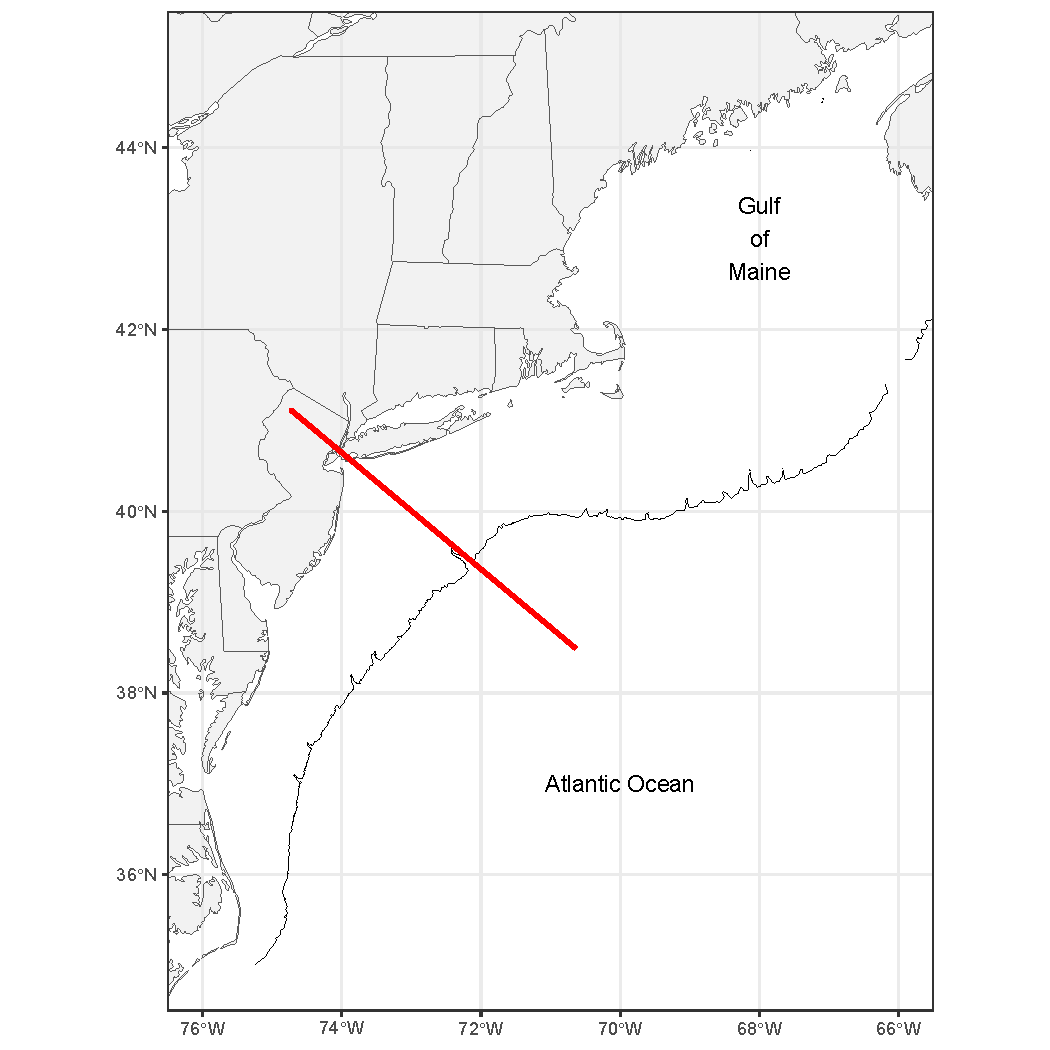
\includegraphics[width=1\linewidth]{map} 

}

\caption{The Northwest Atlantic coastal area where the \DIFdelbeginFL \DIFdelFL{NEUS }\DIFdelendFL \DIFaddbeginFL \DIFaddFL{Northeast US }\DIFaddendFL black sea bass stock occurs. \DIFdelbeginFL \DIFdelFL{Red }\DIFdelendFL \DIFaddbeginFL \DIFaddFL{The red }\DIFaddendFL line indicates the Hudson Canyon delineation of northern and southern regions and spawning populations (after Miller et al. 2016a) and the bathymetric contour is the 400 m isocline.}\label{fig:map}
\end{figure}
\pagebreak

\begin{figure}

{\centering 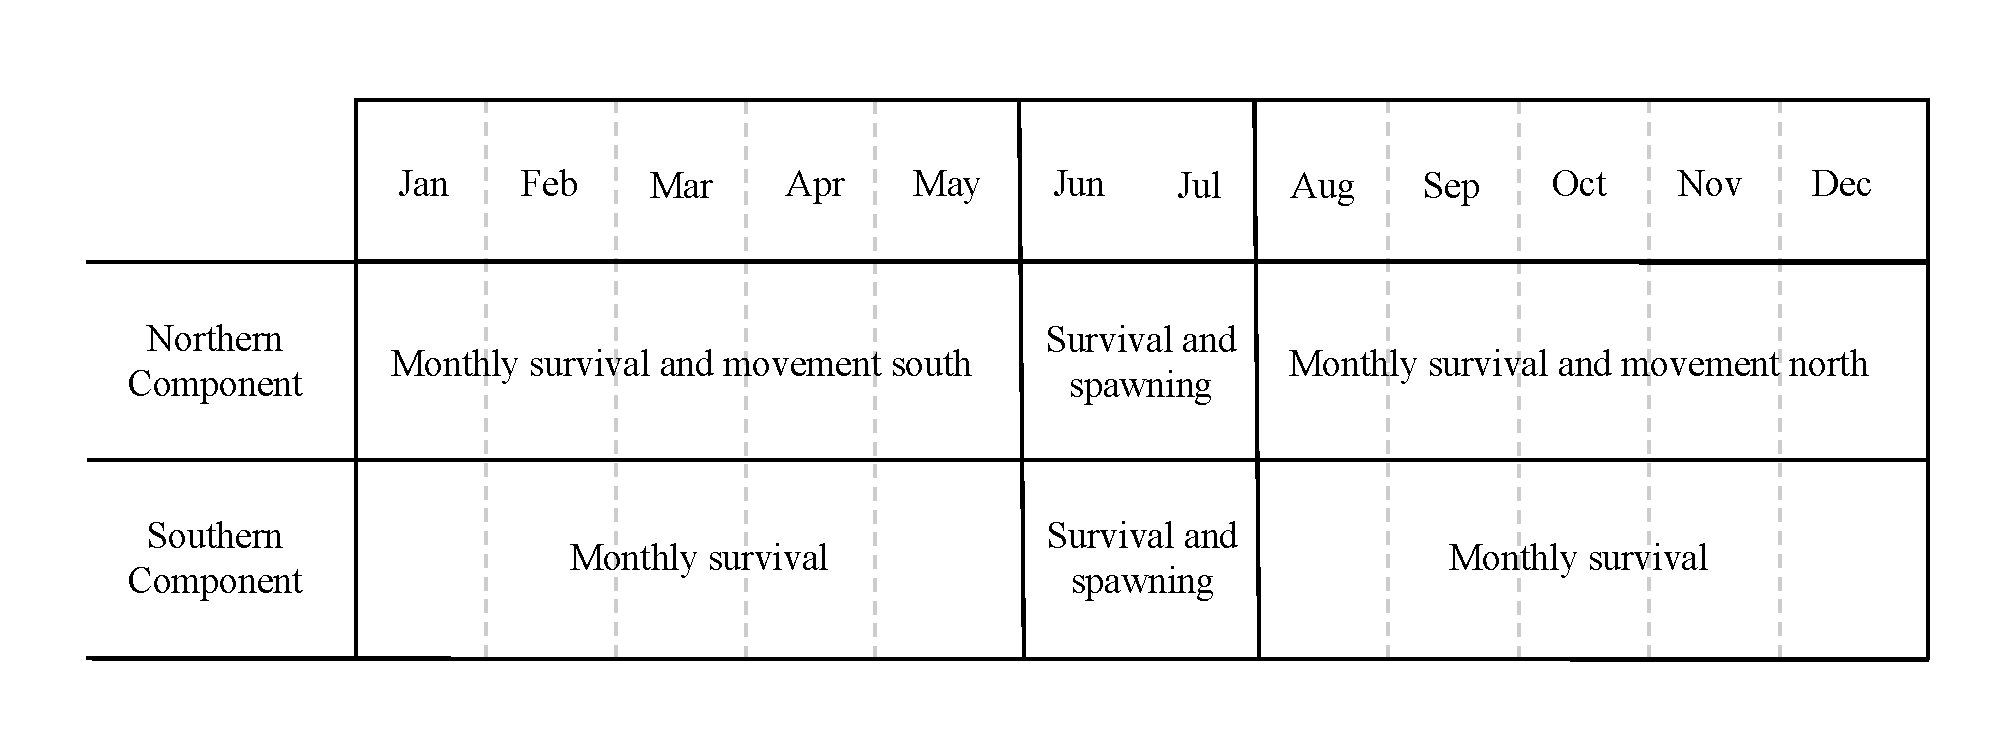
\includegraphics[width=0.8\linewidth]{bsb_movement_diagram} 

}

\caption{Diagram of intervals within the year and configuation of the dynamics of each component of the \DIFdelbeginFL \DIFdelFL{BSB }\DIFdelendFL \DIFaddbeginFL \DIFaddFL{black sea bass }\DIFaddendFL population.}\label{fig:migration-diagram}
\end{figure}
\pagebreak

\begin{figure}

{\centering 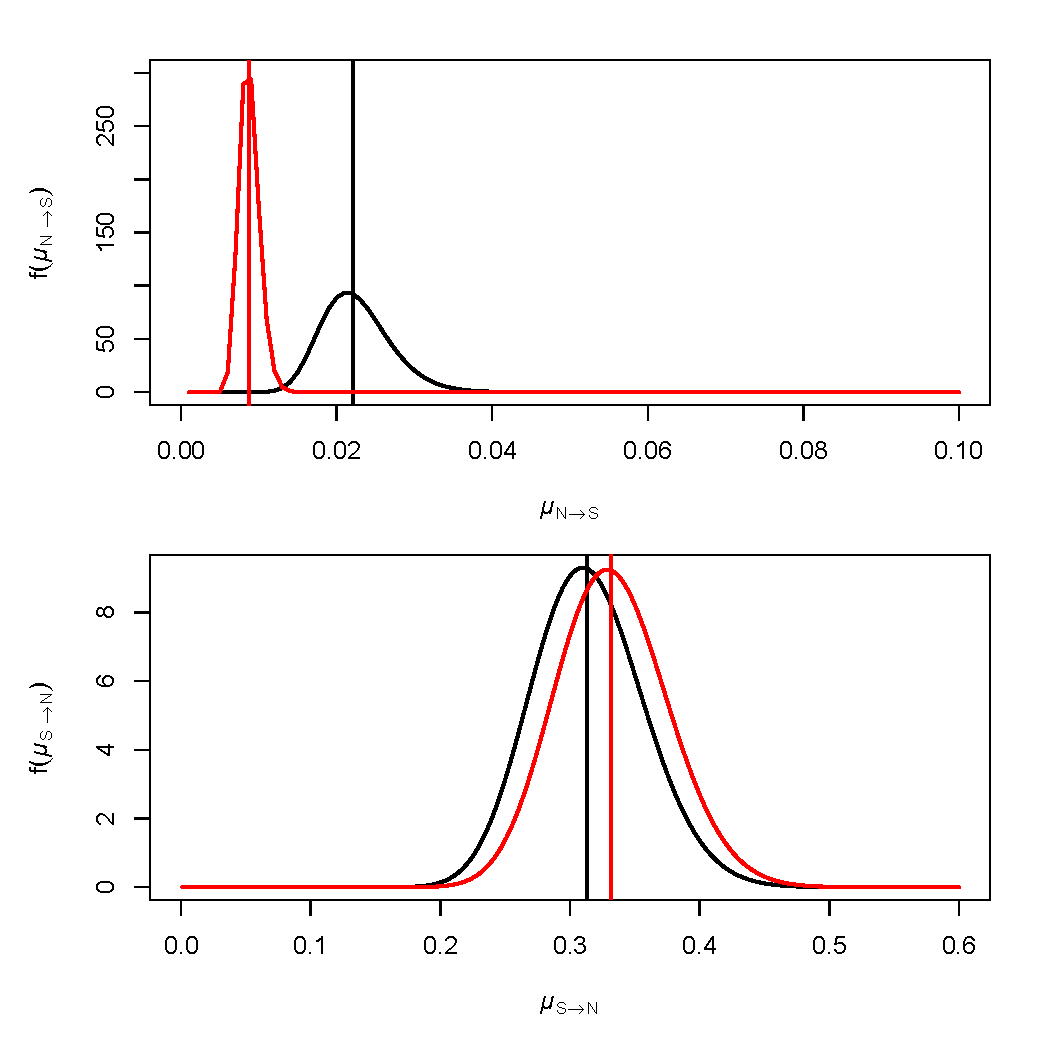
\includegraphics[width=1\linewidth]{move_prior_post} 

}

\caption{Prior (black) and posterior (red) distributions of \DIFaddbeginFL \DIFaddFL{the }\DIFaddendFL movement \DIFdelbeginFL \DIFdelFL{of }\DIFdelendFL \DIFaddbeginFL \DIFaddFL{parameter for }\DIFaddendFL the northern stock component from north to south (top) and south to north (bottom). Vertical lines \DIFdelbeginFL \DIFdelFL{are }\DIFdelendFL \DIFaddbeginFL \DIFaddFL{indicate }\DIFaddendFL the prior and posterior estimates.}\label{fig:move-prior-posterior}
\end{figure}
\pagebreak

\begin{figure}

{\centering 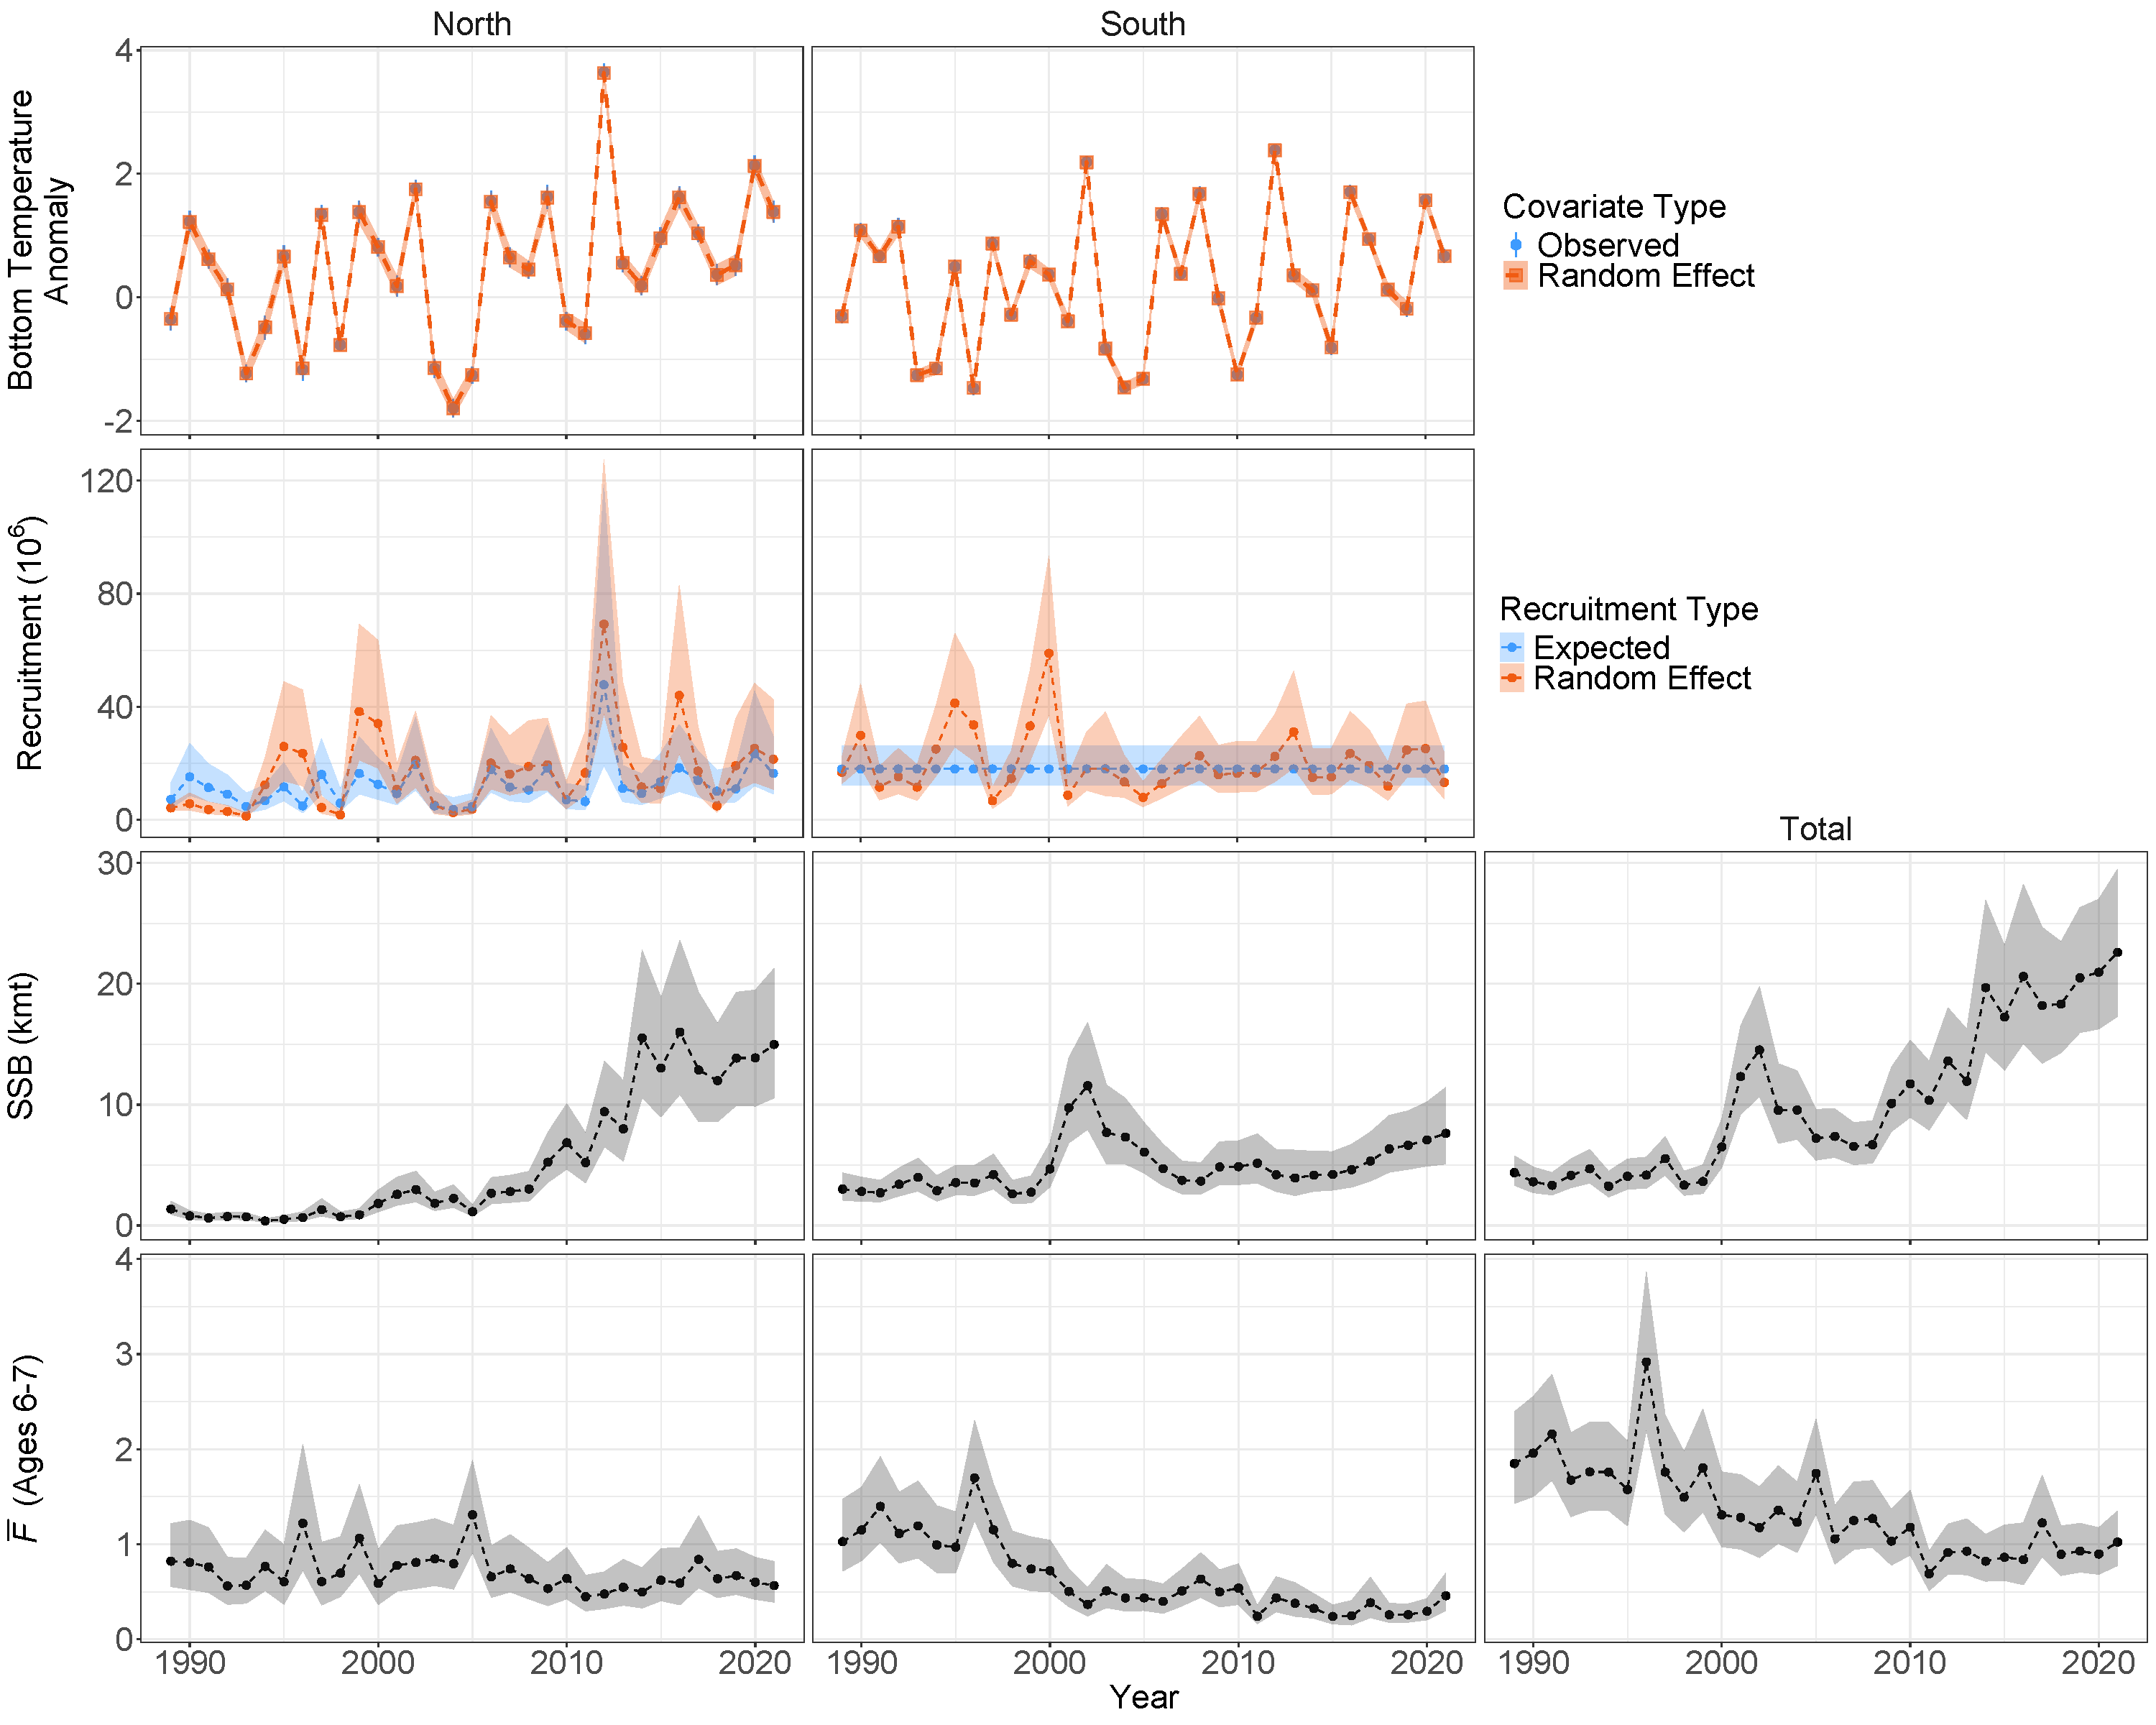
\includegraphics[height=0.95\textheight]{E_R_SSB_F_fig} 

}

\caption{Annual observations and posterior estimates of bottom temperature anomalies (top row), annual expected and random effect recruitment estimates (second row) and SSB and average fishing mortality at ages 6 and 7 from model $M_1$. Columns define estimates regionally (spawning region for SSB) and \DIFdelbeginFL \DIFdelFL{toal }\DIFdelendFL \DIFaddbeginFL \DIFaddFL{total }\DIFaddendFL SSB and fishing mortality across regions. Polygons and vertical lines represent 95\% confidence intervals.}\label{fig:E-R-SSB-F}
\end{figure}
\pagebreak

\begin{figure}

{\centering 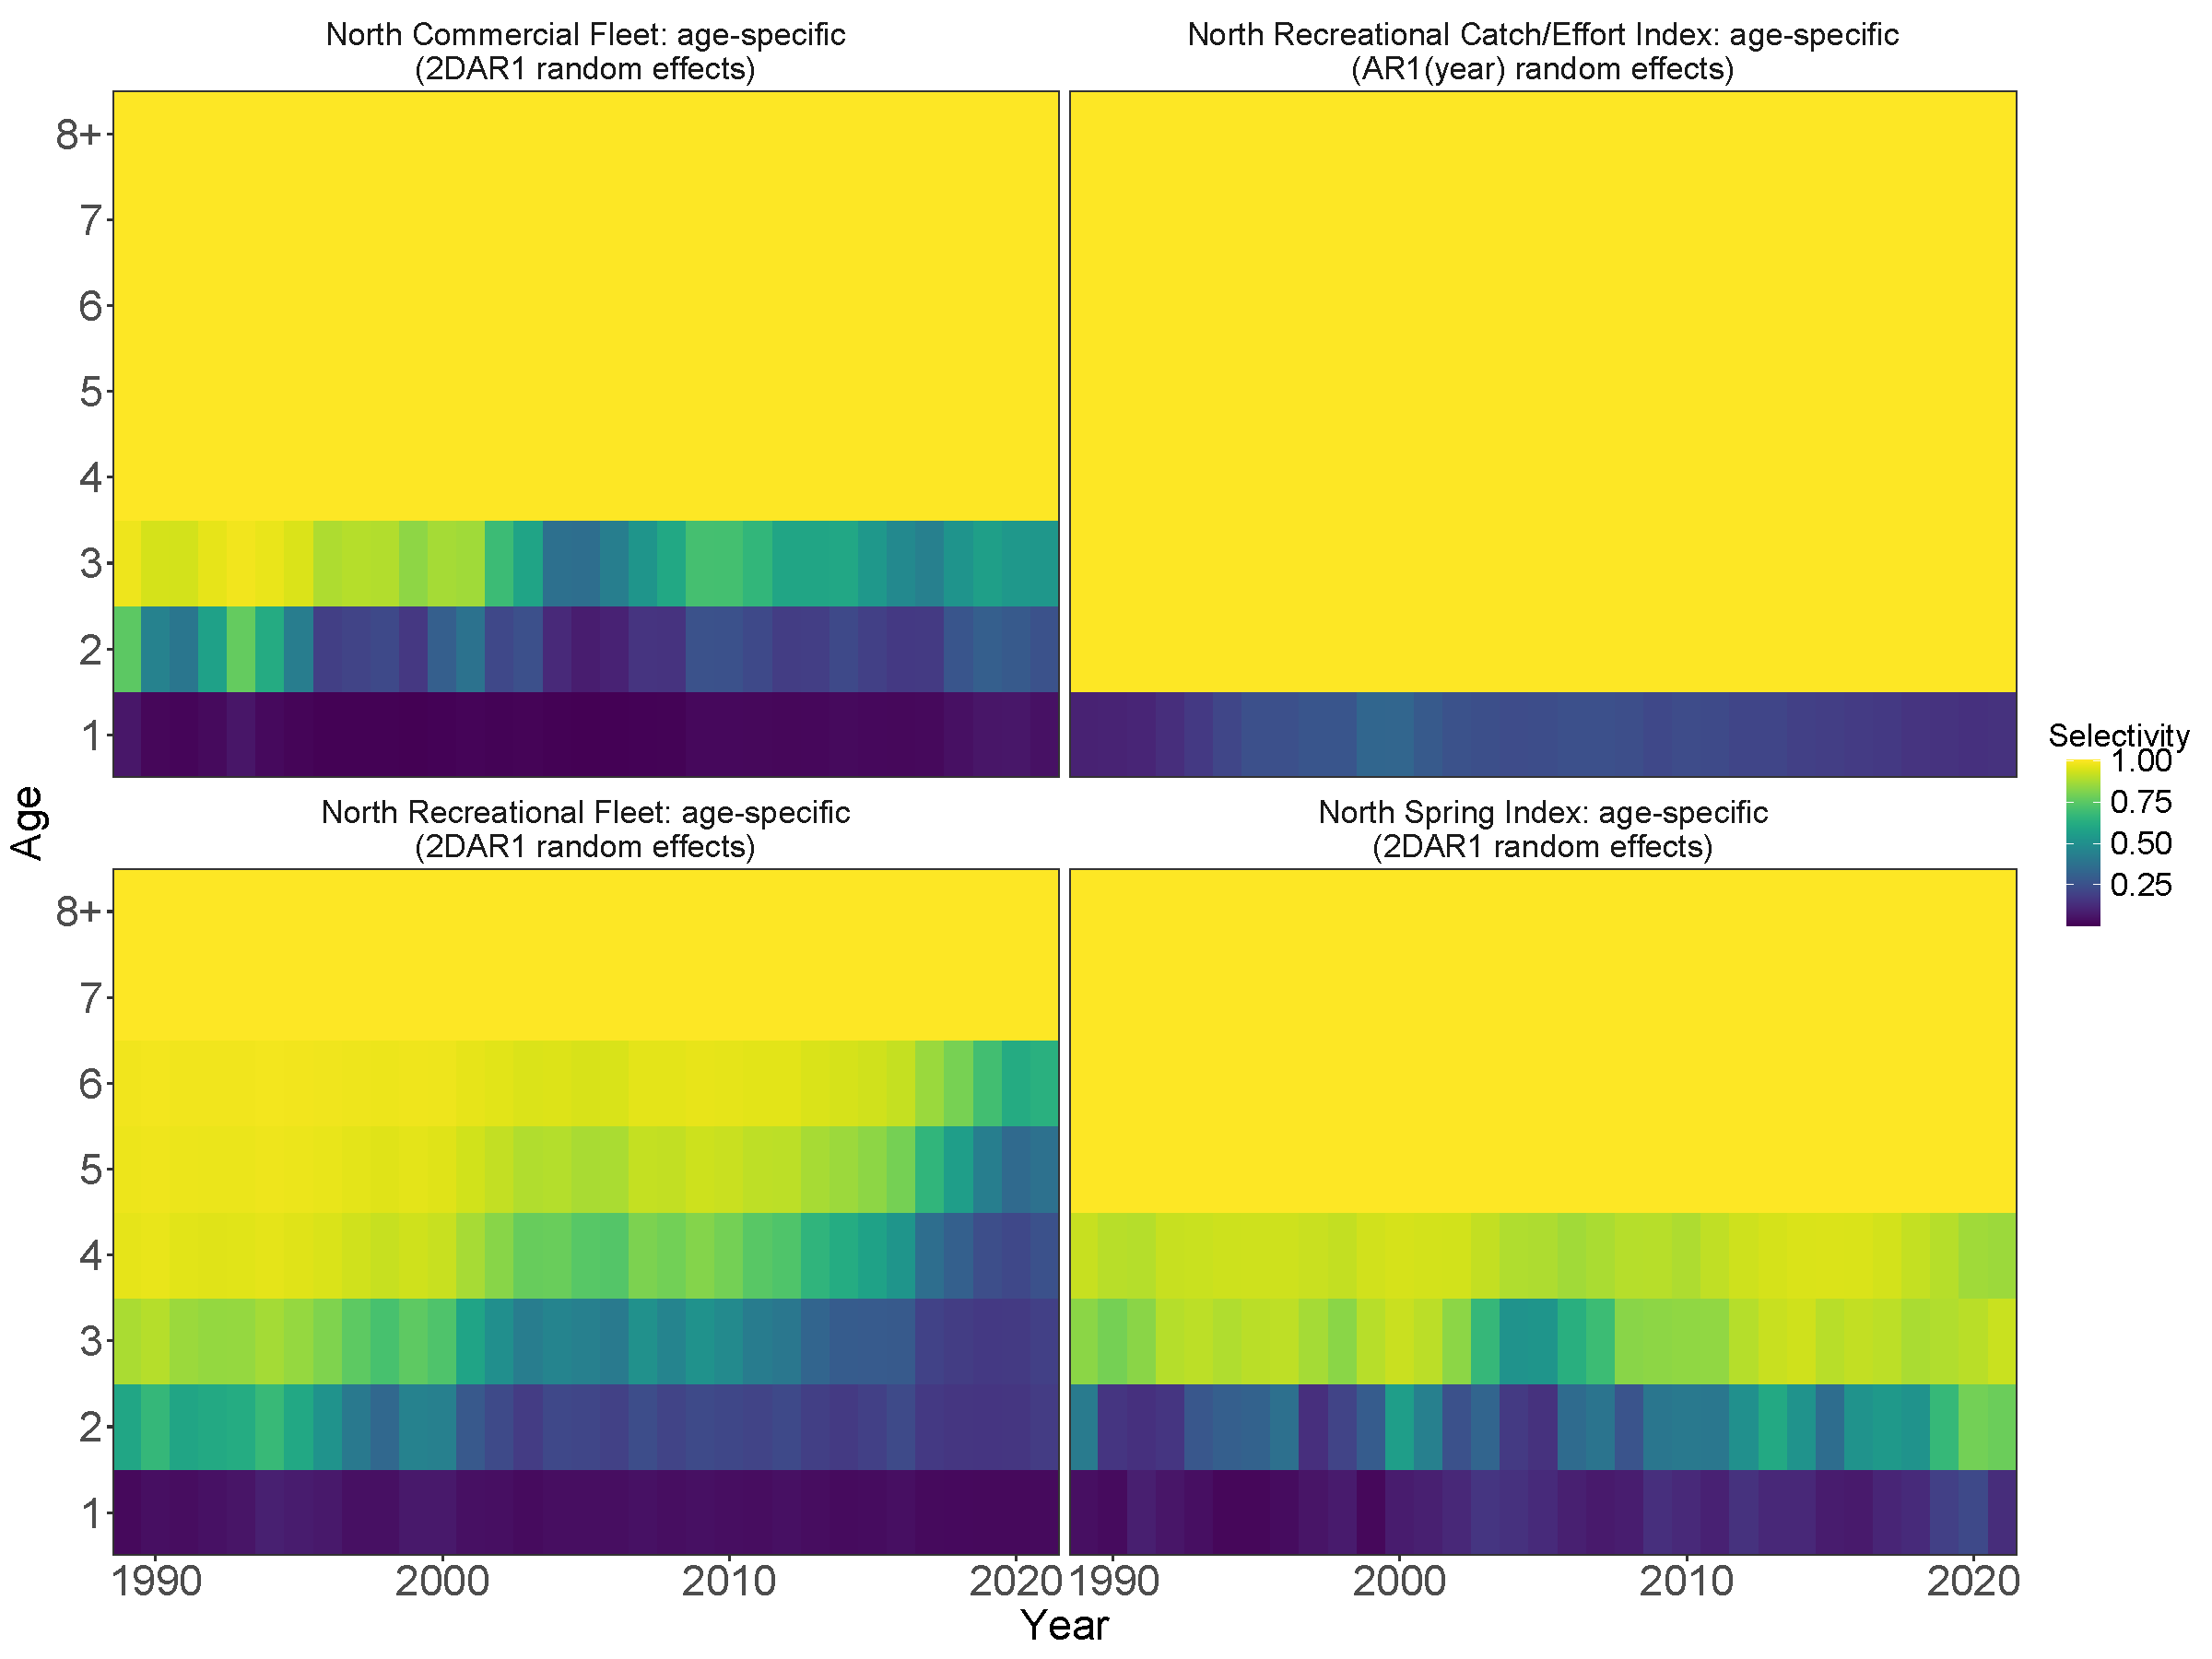
\includegraphics[height=0.95\textheight]{selectivity_re_plot} 

}

\caption{Time and age-varying selectivty for fleets and indices in the northern region with autoregressive random effects.}\label{fig:selectivity-re}
\end{figure}
\pagebreak

\begin{figure}

{\centering 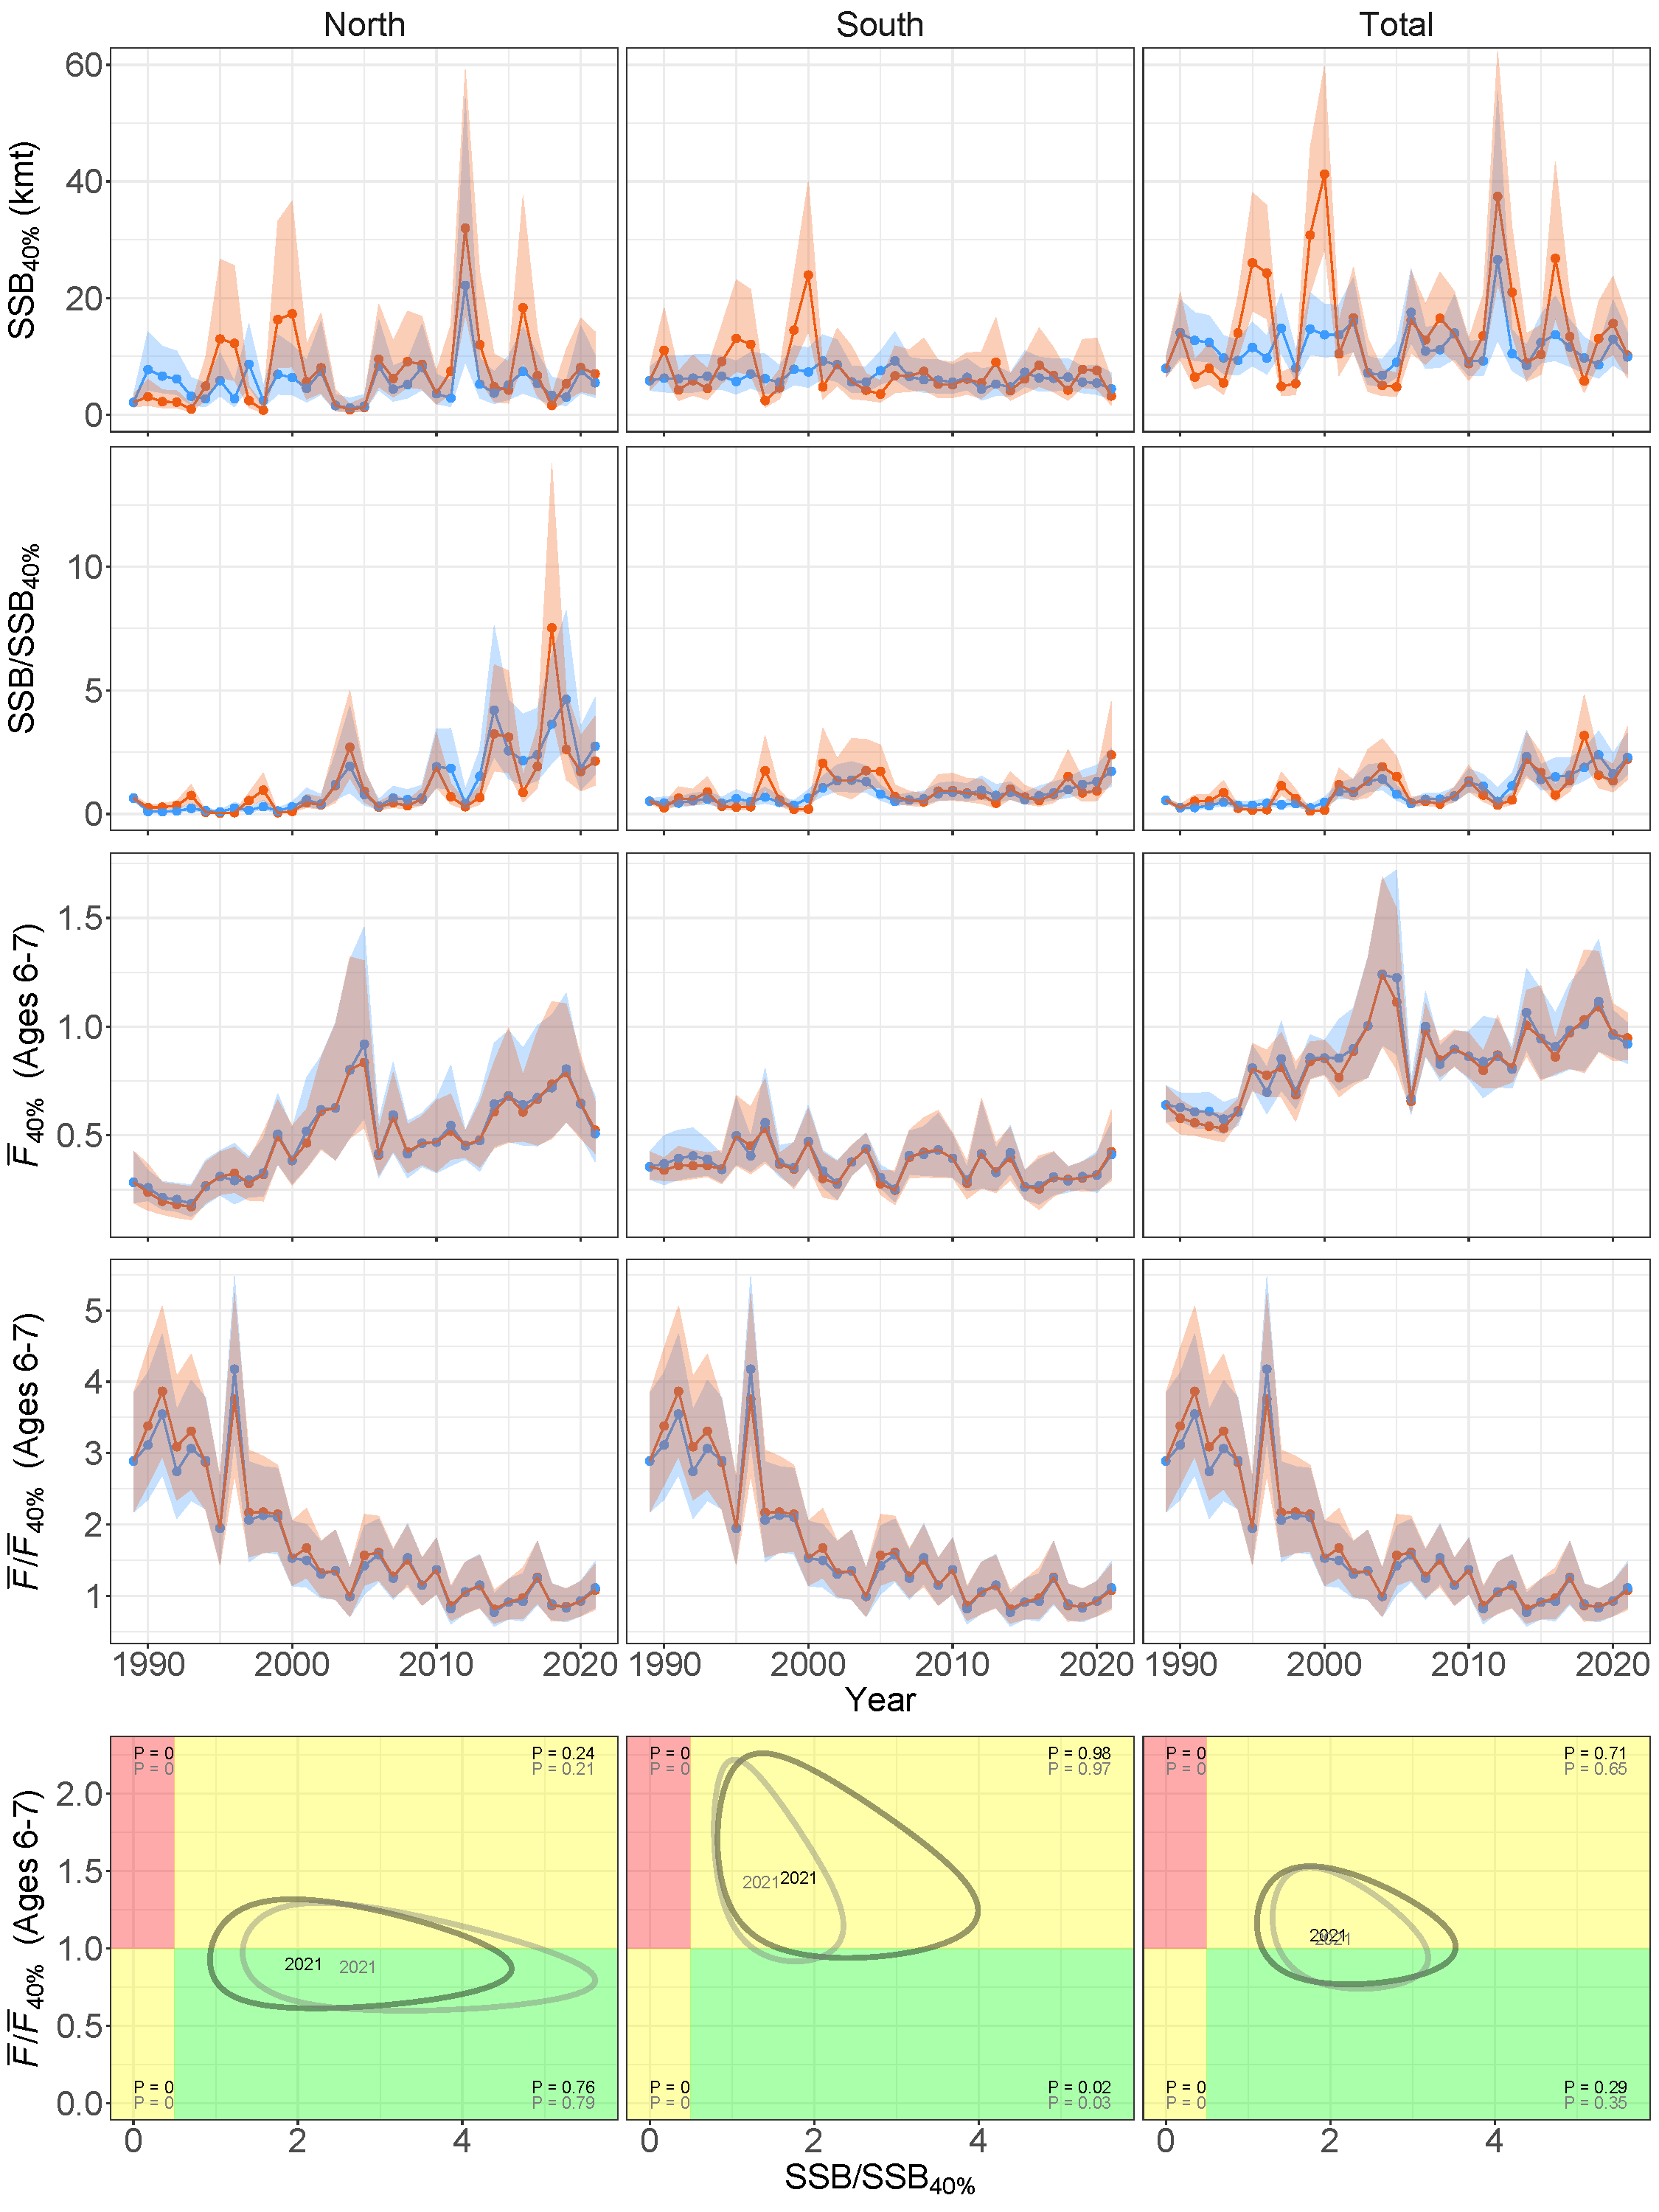
\includegraphics[height=0.85\textheight]{brp_status_results} 

}

\caption{Estimates of average equilibrium $F$ at ages 6 and 7 that produces the 40\% spawning potential ratio \DIFaddbeginFL \DIFaddFL{($F_{40\%}$)}\DIFaddendFL , equilibrium SSB at $F_{40\%}$ based on annual inputs to $\upphi(\widetilde{F})$ calculations, annual fishing and biomass status (ratios), and bivariate kobe plots of status in 2021 where reference points represent prevailing conditions with inputs to $\upphi(\widetilde{F})$ averaged over the last 5 years and recruitment is averaged over the time series. Red and blue in first 4 rows and black and gray in final row indicate alternative annual estimates of recruitment (random effect or expected). All results are based on model $M_1$. Polygons represent 95\% confidence intervals or regions.}\label{fig:annual-BRPs}
\end{figure}

\begin{figure}

{\centering 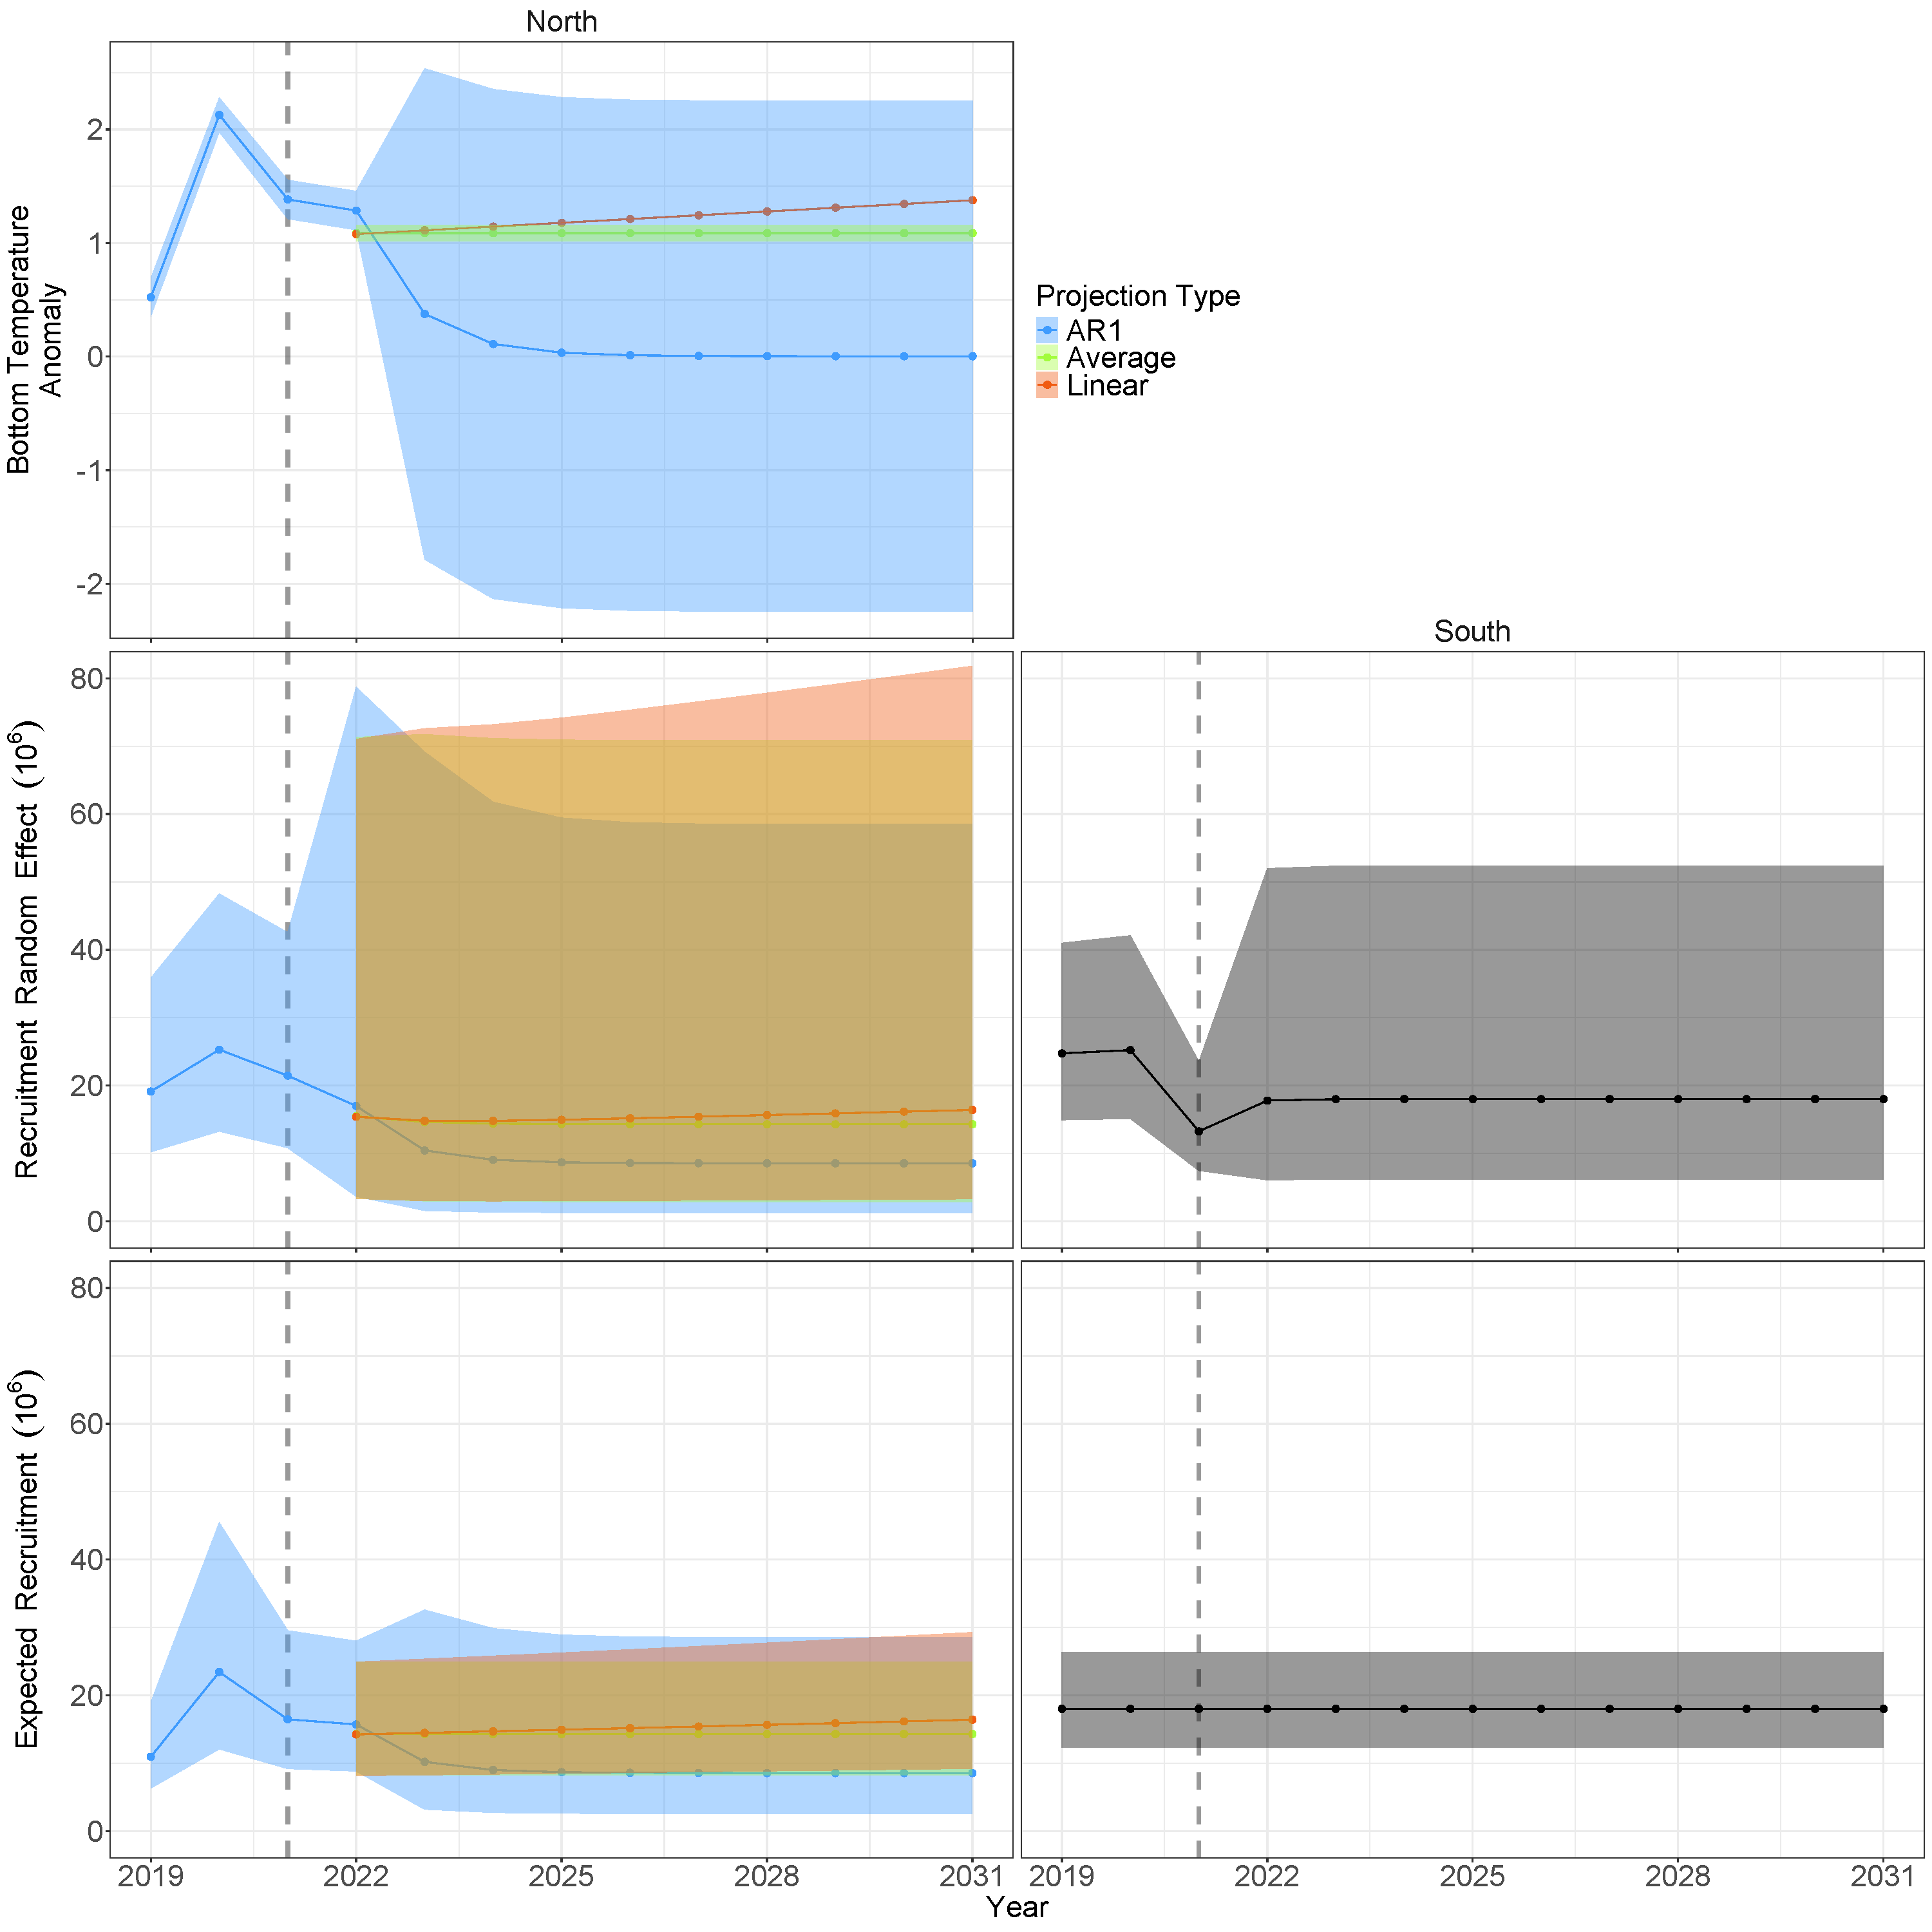
\includegraphics[height=0.95\textheight]{proj_ecov_Recruit_results} 

}

\caption{Annual estimates of bottom temperature in the northern region and alternative recruitment estimates (random effect or expected) by region. Estimates from years after 2021 are from projections of model \DIFdelbeginFL \DIFdelFL{$M1$ }\DIFdelendFL \DIFaddbeginFL \DIFaddFL{$M_1$ }\DIFaddendFL under three alternative assumptions for the bottom temperature anomalies in the northern region. Vertical dotted \DIFdelbeginFL \DIFdelFL{line is }\DIFdelendFL \DIFaddbeginFL \DIFaddFL{lines indicate }\DIFaddendFL the last year of data and polygons represent 95\% confidence intervals.}\label{fig:R-BT-proj}
\end{figure}

\begin{figure}

{\centering 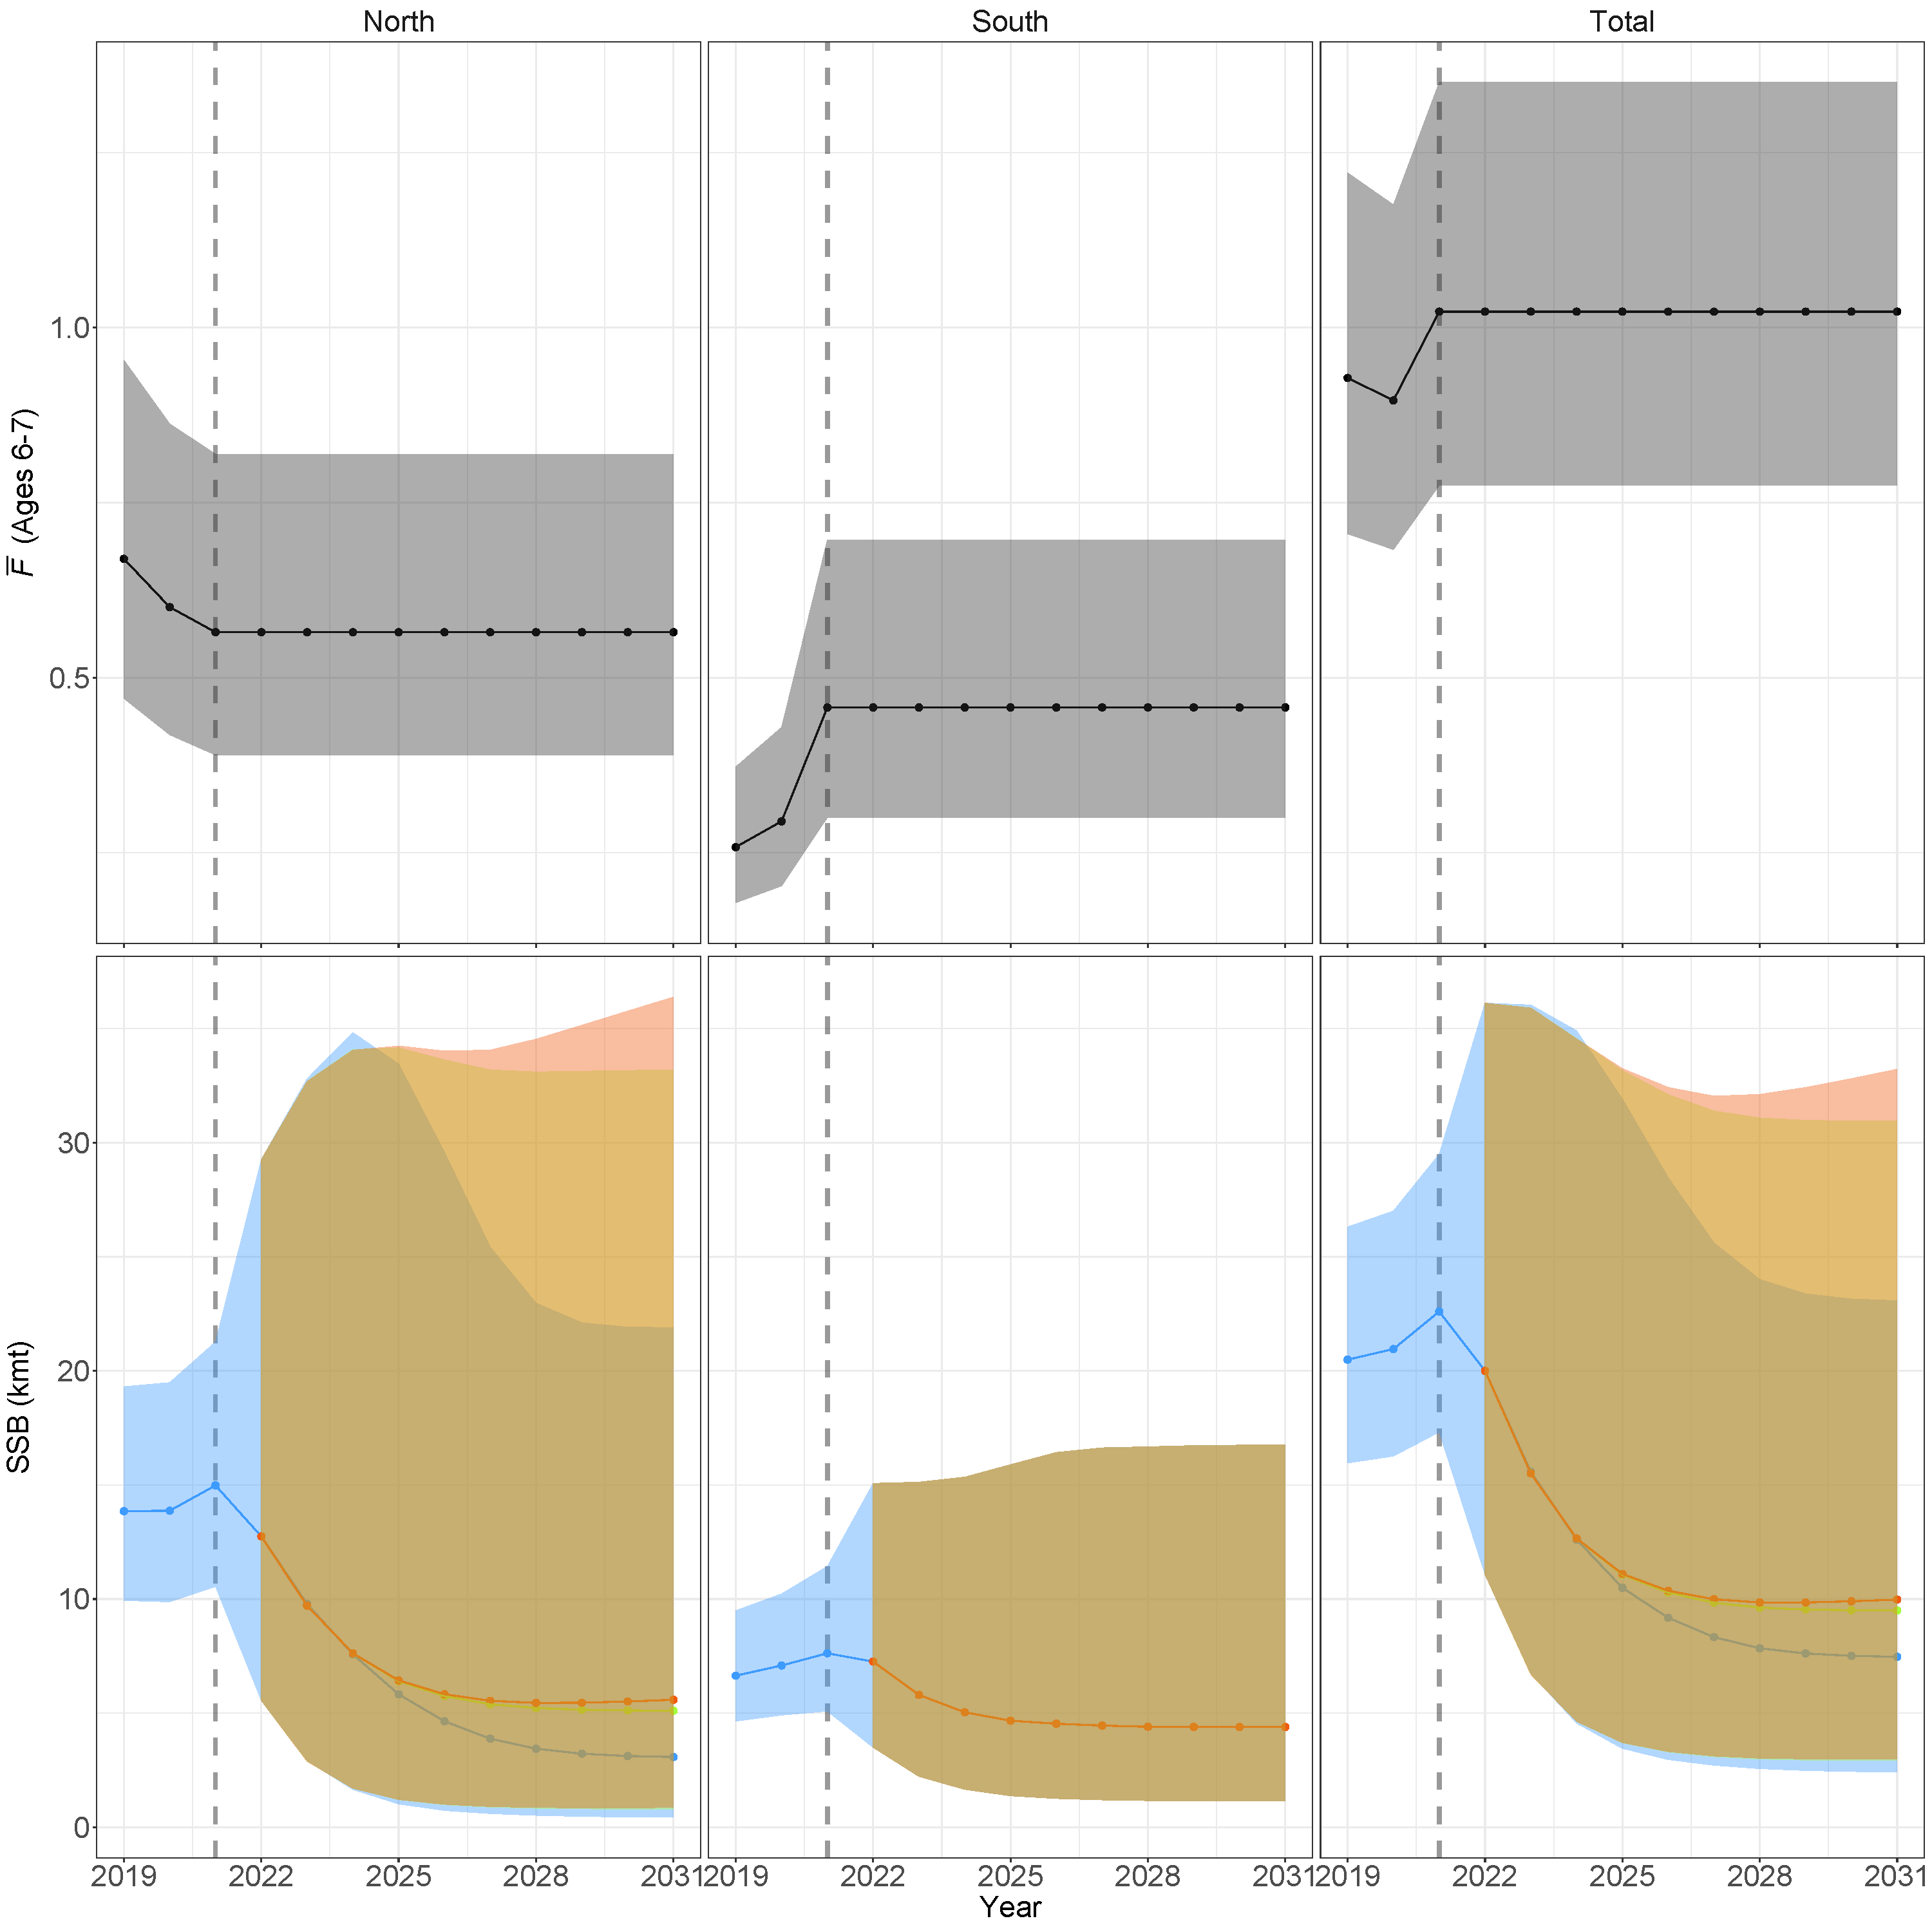
\includegraphics[height=0.95\textheight]{proj_F_SSB} 

}

\caption{Annual estimates of average fishing mortality and SSB by region and in total. Estimates in years beyond 2021 are from projecting model $M_1$ under alternative assumptions for bottom temperature anomalies in the northern region. Vertical dotted \DIFdelbeginFL \DIFdelFL{line is }\DIFdelendFL \DIFaddbeginFL \DIFaddFL{lines indicate }\DIFaddendFL the last year of data and polygons represent 95\% confidence intervals.}\label{fig:F-SSB-proj}
\end{figure}

\begin{landscape}

\begin{figure}

{\centering 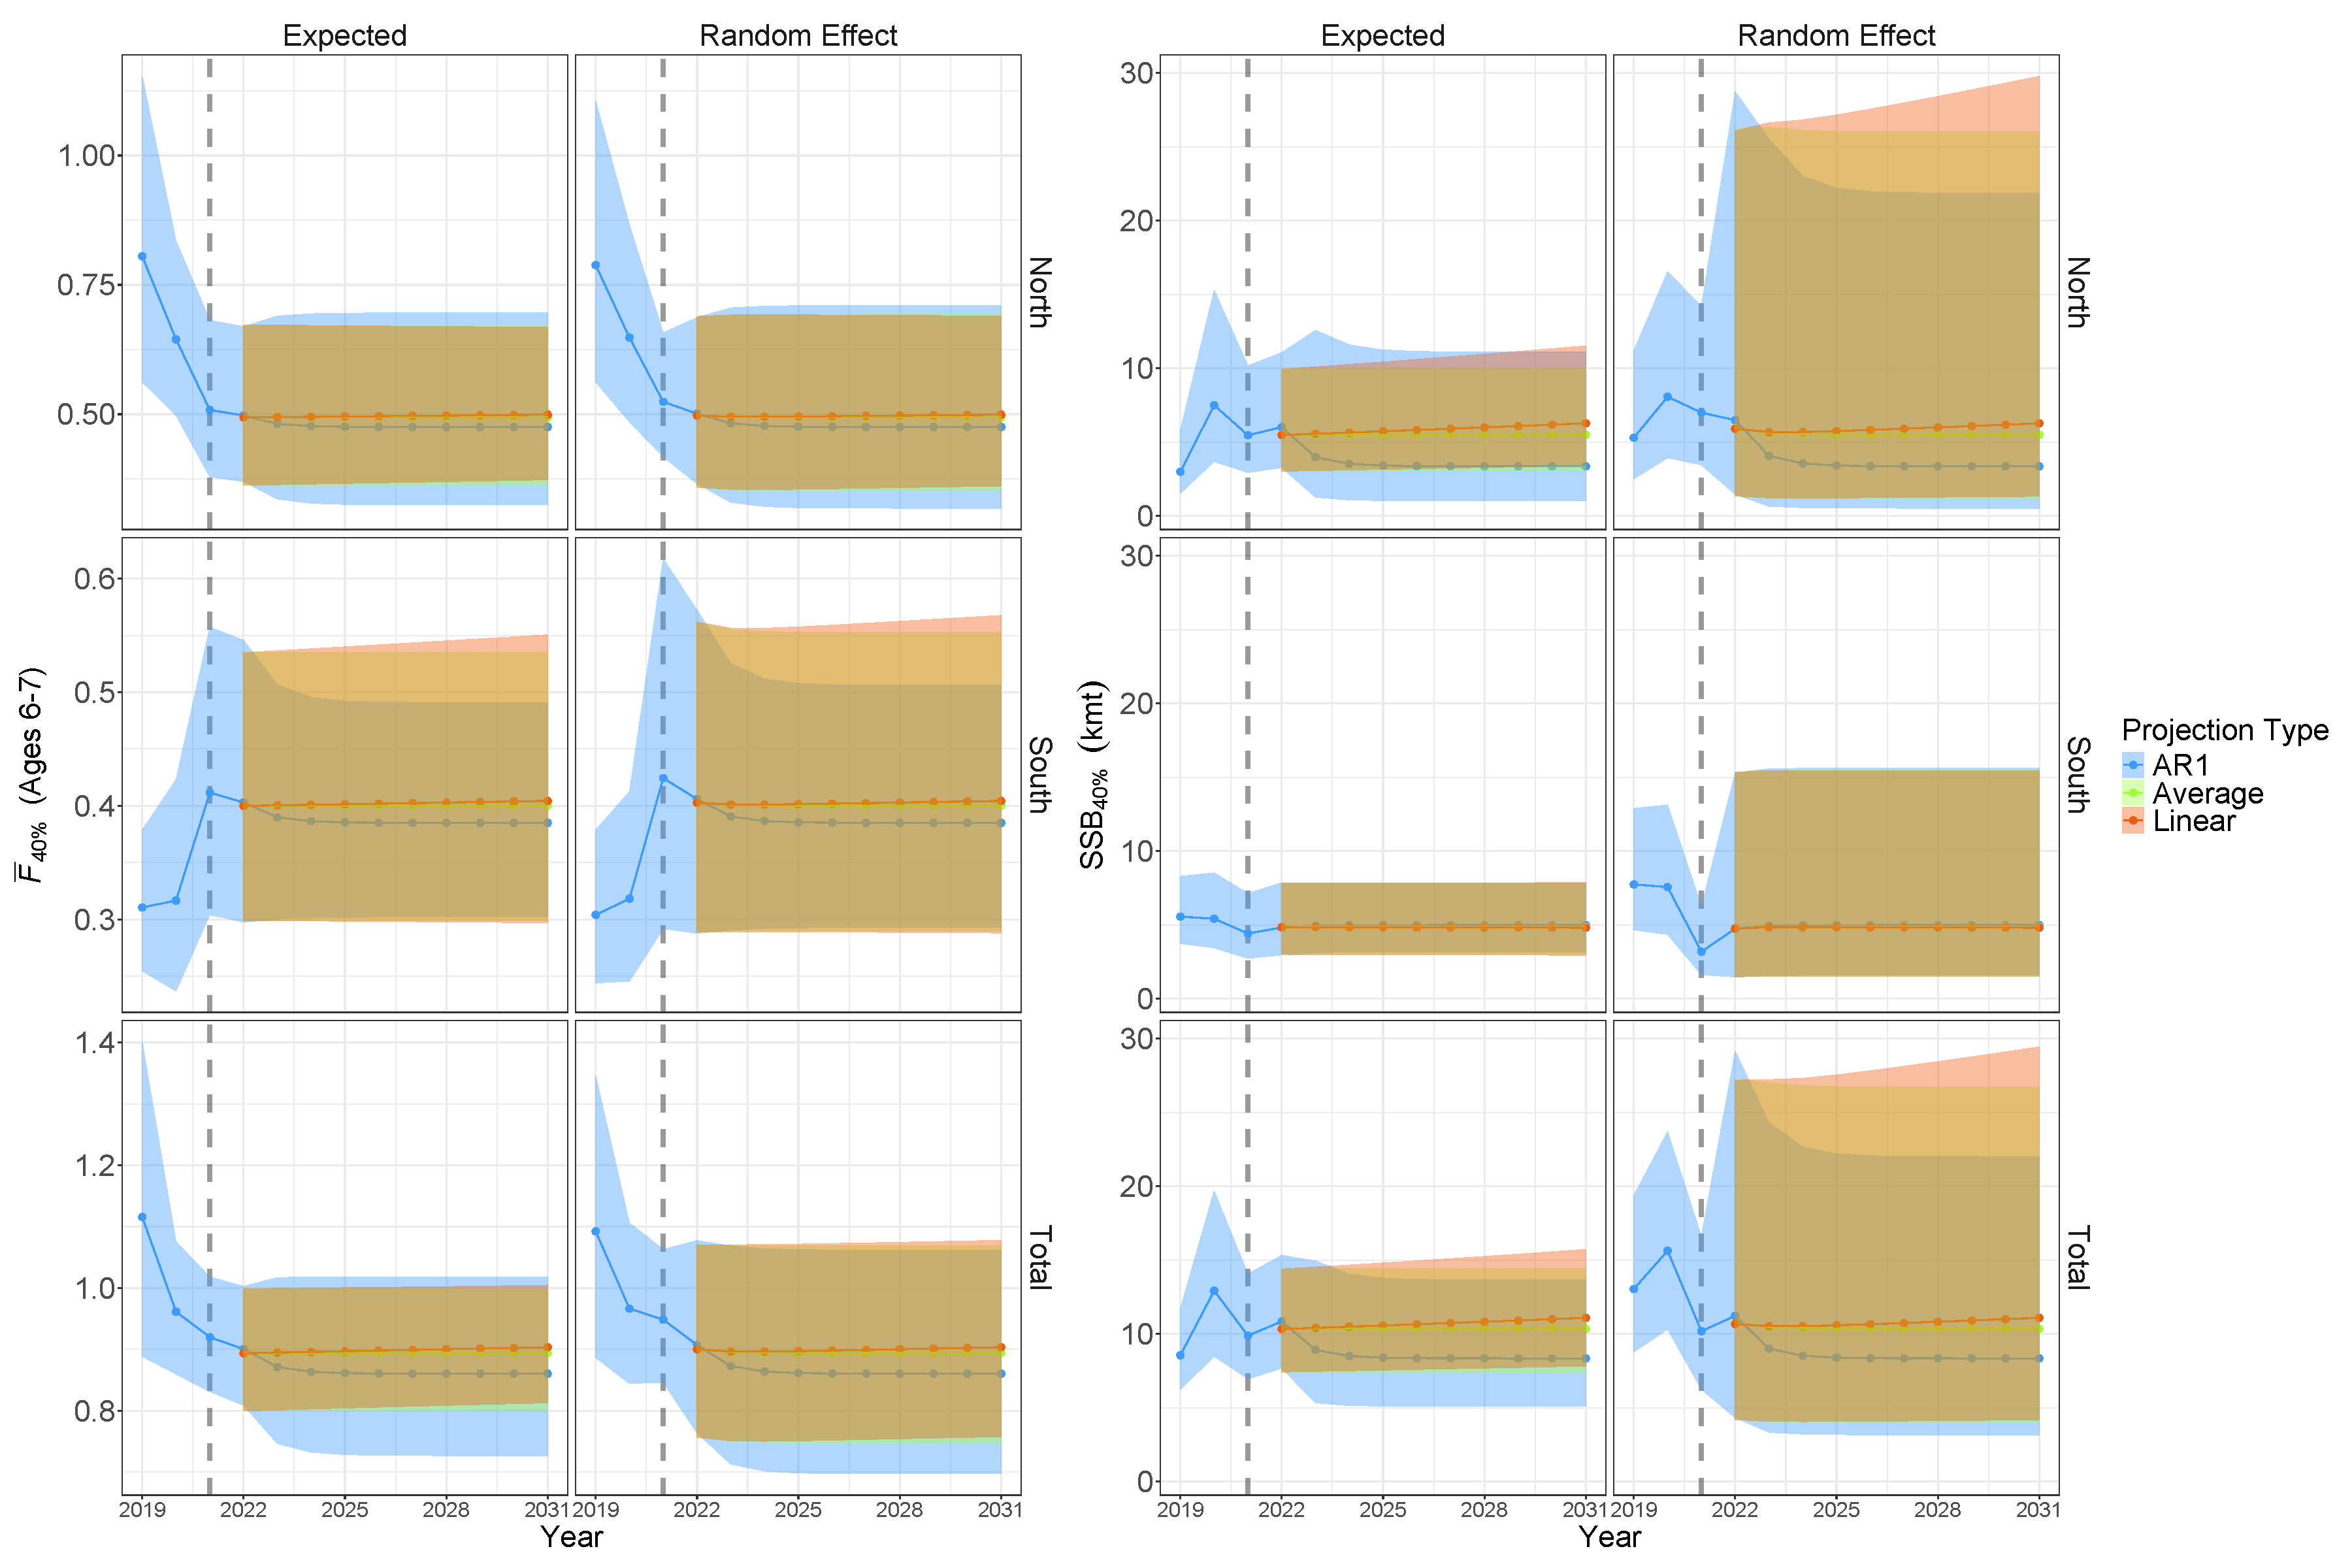
\includegraphics[height=0.95\textheight]{proj_brps} 

}

\caption{Annual estimates by region and in total of average equilibrium $F$ at ages 6 and 7 that produces the 40\% spawning potential ratio and SSB at $F_{40\%}$. Estimates in years beyond 2021 are from projecting model $M_1$ under alternative assumptions for bottom temperature anomalies in the northern region and average $\upphi(\widetilde{F})$ inputs from the last 5 years of the unprojected model. Vertical dotted \DIFdelbeginFL \DIFdelFL{line is }\DIFdelendFL \DIFaddbeginFL \DIFaddFL{lines indicate }\DIFaddendFL the last year of data and polygons represent 95\% confidence intervals.}\label{fig:brps-proj}
\end{figure}

\end{landscape}

\clearpage

\setcounter{table}{0}
\renewcommand\thetable{\arabic{table}}

\hypertarget{tables}{%
\section*{Tables}\label{tables}}
\addcontentsline{toc}{section}{Tables}

\begin{table}[!h]
\centering
\caption{\label{tab:model-desc-table}Assumptions for temperature effects and random effects for age 1 natural mortality \DIFaddbeginFL \DIFaddFL{rates ($M$) }\DIFaddendFL for each model.}
\centering
\begin{tabular}[t]{llll}
\toprule
\multicolumn{1}{c}{ } & \multicolumn{2}{c}{Temperature Effect} & \multicolumn{1}{c}{ } \\
\cmidrule(l{3pt}r{3pt}){2-3}
Model & North & South & $M$ at age 1 random effects\\
\midrule
$M_{0}$ & -- & -- & none\\
$M_{1}$ & Recruitment & -- & none\\
$M_{2}$ & -- & Recruitment & none\\
$M_{3}$ & Recruitment & Recruitment & none\\
$M_{4}$ & $M$ at age 1 & -- & none\\
\addlinespace
$M_{5}$ & -- & $M$ at age 1 & none\\
$M_{6}$ & $M$ at age 1 & $M$ at age 1 & none\\
$M_{7}$ & -- & -- & time-varying\\
$M_{8}$ & Recruitment & -- & time-varying\\
$M_{9}$ & -- & Recruitment & time-varying\\
\addlinespace
$M_{10}$ & Recruitment & Recruitment & time-varying\\
$M_{11}$ & $M$ at age 1 & -- & time-varying\\
$M_{12}$ & -- & $M$ at age 1 & time-varying\\
$M_{13}$ & $M$ at age 1 & $M$ at age 1 & time-varying\\
\bottomrule
\end{tabular}
\end{table}

\begin{table}

\caption{\label{tab:diff-aic-table}Difference between AIC and the lowest AIC for each model by retrospective peel.}
\centering
\begin{tabular}[t]{lrrrrrrrr}
\toprule
\multicolumn{1}{c}{ } & \multicolumn{8}{c}{Peel} \\
\cmidrule(l{3pt}r{3pt}){2-9}
Model & 0 & 1 & 2 & 3 & 4 & 5 & 6 & 7\\
\midrule
$M_{0}$ & 11.83 & 11.39 & 10.41 & 10.05 & 9.86 & 9.41 & 8.47 & 8.22\\
$M_{1}$ & 0.00 & 0.00 & 0.00 & 0.00 & 0.00 & 0.00 & 0.00 & 0.00\\
$M_{2}$ & 12.63 & 12.03 & 11.41 & 11.06 & 10.91 & 10.34 & 9.20 & 9.22\\
$M_{3}$ & 0.80 & 0.64 & 1.00 & 1.01 & 1.05 & 0.93 & 0.73 & 1.00\\
$M_{4}$ & 13.81 & 13.35 & 12.26 & 11.82 & 11.71 & 11.18 & 10.08 & 9.85\\
\addlinespace
$M_{5}$ & 13.25 & 12.55 & 11.68 & 11.21 & 11.07 & 10.41 & 9.86 & 9.71\\
$M_{6}$ & 15.22 & 14.51 & 13.52 & 12.97 & 12.91 & 12.17 & 11.46 & 11.33\\
$M_{7}$ & 14.32 & 13.75 & 12.17 & 11.30 & 11.43 & 10.55 & 9.71 & 9.42\\
$M_{8}$ & 2.25 & 2.10 & 1.47 & 0.96 & 1.29 & 0.91 & 0.98 & 0.99\\
$M_{9}$ & 15.12 & 14.39 & 13.17 & 12.31 & 12.48 & 11.49 & 10.44 & 10.43\\
\addlinespace
$M_{10}$ & 3.05 & 2.74 & 2.47 & 1.97 & 2.34 & 1.84 & 1.71 & 1.99\\
$M_{11}$ & 16.29 & 15.74 & 14.17 & 13.30 & 13.43 & 12.55 & 11.68 & 11.39\\
$M_{12}$ & 15.73 & 14.91 & 13.43 & 12.46 & 12.64 & 11.55 & 11.10 & 10.92\\
$M_{13}$ & 17.70 & 16.91 & 15.43 & 14.46 & 14.64 & 13.55 & 13.07 & 12.88\\
\bottomrule
\end{tabular}
\end{table}

\begin{table}

\caption{\label{tab:rho-table}Mohn's $\rho$ for SSB, and average F at ages 6 and 7 in northern and southern regions.}
\centering
\begin{tabular}[t]{lrrrr}
\toprule
\multicolumn{1}{c}{ } & \multicolumn{2}{c}{SSB} & \multicolumn{2}{c}{Average F} \\
\cmidrule(l{3pt}r{3pt}){2-3} \cmidrule(l{3pt}r{3pt}){4-5}
Model & North & South & North & South\\
\midrule
$M_{0}$ & -0.040 & -0.023 & 0.041 & -0.048\\
$M_{1}$ & -0.040 & -0.023 & 0.041 & -0.048\\
$M_{2}$ & -0.040 & -0.024 & 0.041 & -0.047\\
$M_{3}$ & -0.040 & -0.024 & 0.041 & -0.047\\
$M_{4}$ & -0.041 & -0.022 & 0.042 & -0.048\\
\addlinespace
$M_{5}$ & -0.041 & -0.023 & 0.042 & -0.048\\
$M_{6}$ & -0.042 & -0.023 & 0.042 & -0.048\\
$M_{7}$ & -0.042 & -0.022 & 0.043 & -0.048\\
$M_{8}$ & -0.044 & -0.023 & 0.044 & -0.048\\
$M_{9}$ & -0.042 & -0.024 & 0.043 & -0.048\\
\addlinespace
$M_{10}$ & -0.044 & -0.024 & 0.044 & -0.047\\
$M_{11}$ & -0.041 & -0.022 & 0.042 & -0.048\\
$M_{12}$ & -0.042 & -0.023 & 0.043 & -0.048\\
$M_{13}$ & -0.041 & -0.023 & 0.042 & -0.048\\
\bottomrule
\end{tabular}
\end{table}
\begin{table}

\caption{\label{tab:beta-sig-peel-table}Estimates of temperature effects on recruitment and variance and autocorrelation parameters for recruitment for northern ($N$) and southern ($S$) components for models with no effects ($M_0$), effects on specific components ($M_1$ and $M_2$) or both components simultaneously ($M_3$) from the full model (Peel 0) and each retrospective peel.}
\centering
\begin{tabular}[t]{lrrrrrrrr}
\toprule
\multicolumn{1}{c}{ } & \multicolumn{8}{c}{Peel} \\
\cmidrule(l{3pt}r{3pt}){2-9}
Parameter & 0 & 1 & 2 & 3 & 4 & 5 & 6 & 7\\
\midrule
$M_{1}$ $\widehat{\beta}_{R,N}$ & 0.474 & 0.480 & 0.485 & 0.476 & 0.464 & 0.468 & 0.439 & 0.445\\
$M_{2}$ $\widehat{\beta}_{R,S}$ & 0.099 & 0.105 & 0.094 & 0.095 & 0.092 & 0.096 & 0.099 & 0.091\\
$M_{3}$ $\widehat{\beta}_{R,N}$ & 0.474 & 0.480 & 0.485 & 0.476 & 0.464 & 0.468 & 0.439 & 0.445\\
$M_{3}$ $\widehat{\beta}_{R,S}$ & 0.099 & 0.105 & 0.094 & 0.095 & 0.092 & 0.096 & 0.099 & 0.091\\
$M_{0}$ Conditional $\widehat{\sigma}_{R,N}$ & 0.925 & 0.953 & 0.978 & 0.988 & 0.978 & 1.010 & 0.981 & 1.007\\
\addlinespace
$M_{1}$ Conditional $\widehat{\sigma}_{R,N}$ & 0.730 & 0.752 & 0.780 & 0.786 & 0.775 & 0.801 & 0.785 & 0.800\\
$M_{0}$ $\widehat{\rho}_{R,N}$ & 0.362 & 0.375 & 0.385 & 0.405 & 0.424 & 0.432 & 0.427 & 0.431\\
$M_{1}$ $\widehat{\rho}_{R,N}$ & 0.296 & 0.307 & 0.334 & 0.373 & 0.394 & 0.406 & 0.428 & 0.429\\
$M_{0}$ Marginal $\widehat{\sigma}_{R,N}$ & 0.992 & 1.028 & 1.060 & 1.080 & 1.081 & 1.120 & 1.084 & 1.117\\
$M_{1}$ Marginal $\widehat{\sigma}_{R,N}$ & 0.764 & 0.791 & 0.827 & 0.848 & 0.843 & 0.877 & 0.869 & 0.885\\
\bottomrule
\end{tabular}
\end{table}

\clearpage

\hypertarget{appendix-a}{%
\section*{Appendix A}\label{appendix-a}}
\addcontentsline{toc}{section}{Appendix A}

\setcounter{table}{0}
\renewcommand\thetable{A\arabic{table}}
\begin{longtable}[c]{r p{0.85\textwidth}}
\caption{Definition of terms.\label{symbols}}%
\\ \hline \hline \endfirsthead 
\caption[]{(Continued)} %
\\ \hline \hline \endhead
 \hline \hline \endfoot
$a$ & Age class indicator\\
$A$ & Last age class (``plus group'')\\
$a_{y,a,i,r}$ & Hazard (or negative sum of the instantaneous rates of mortality and movement) from the state corresonding to being alive in region $r$ for year $y$, age $a$ and seasonal interval $i$\\
$\mathbf{A}_{y,a,i}$ & Instantaneous rate matrix for seasonal interval $i$, year $y$, and age $a$ ($(n_R + n_F + 1) \times (n_R + n_F + 1)$)\\
$\mathbf{c}_{a}$ & Vector (length $n_F$) of mean individual weight at age $a$ for each fleet to use for $\upnu(\widetilde{F})$\\
$\mathbf{c}_{y,a}$ & Vector (length $n_F$) of mean individual weight at age $a$ in year $y$ for each fleet\\
$C_{f,y}$ & Observed aggregate catch for fleet $f$ in year $y$\\
$\widehat C_{f,y}$ & Predicted aggregate catch for fleet $f$ in year $y$\\
$\widehat{\mathbf{C}}_{y,a}$ & Vector (length $n_F$) of predicted biomass captured at age $a$ in year $y$ by each fleet across all stocks\\
$\widehat{\mathbf{C}}_y$ & Vector (length $n_F$) of predicted aggregate catch for each fleet in year $y$\\
$D_{y,a,i}$ & Proportion dying from natural mortality over the seasonal interval $i$ given alive (1 region model)\\
$\mathbf{D}_{y,a,i}$ & Vector (length $n_R$) of proportions dying from natural mortality over the seasonal interval $i$ given alive  in each region at the start of the interval\\
$f$ & Fishing fleet indicator\\
$F_{f,1,a}$ & Fishing mortality rate at age $a$ for fleet $f$ in the first year\\
$F_{f,y,a,i}$ & Fishing mortality rate for fleet $f$ in year $y$ at age $a$ in seasonal interval $i$\\
$F_{\text{MSY}}$ & Fully-selected fishing mortality rate that maximizes equilibrium yield\\
$\widetilde{F}$ & Equilibrium fully-selected fishing mortality rate parameter for equilibrium spawning-biomass-per-recruit and yield-per-recruit\\
$\widetilde{F}_1$ & Equilibrium fully-selected fishing mortality rate parameter for equilibrium abundance at age in the first year\\
$\widetilde{F}_{f,a}$ & Equilibrium fully-selected fishing mortality rate at age $a$ for fleet $f$ for equilibrium spawning-biomass-per-recruit and yield-per-recruit\\
$\widetilde{F}_{f,1,a}$ & Equilibrium fishing mortality rate at age $a$ for fleet $f$ for equilibrium abundance at age in the first year\\
$\overline{F}_{f,a}$ & Average fishing mortality rate for fleet $f$ at age $a$ over user-specified set of years\\
$g(\mu_{r\rightarrow r',y,a,i})$ & Link function for movement rate $\mu_{r\rightarrow r',y,a,i}$\\
$h(\log \widetilde{F})$ & Function used in Newton-Raphson method to determine reference points\\
$h^{(1)}(\log \widetilde{F})$ & Derivative of $h(\log \widetilde{F})$ with respect to $\log \widetilde{F}$\\
$H_{y,a,i}(r,f)$ & Proportion captured in fleet $f$ given beginning the seasonal interval alive in region $r$ for year $y$, age $a$, and seasonal interval $i$ \\
$\mathbf{H}_{a}$ & Matrix ($n_R \times n_F$) of equilibrium proportions captured from age $a$ to $a+1$ in each fleet (columns) given alive on January 1 in each region (rows)\\
$\mathbf{H}_{y,a,i}$ &  Matrix ($n_R \times n_F$) of proportions captured in each fishing fleet for year $y$, age $a$, and seasonal interval $i$ given alive in region $r$ at the beginning of the interval (submatrix of $\mathbf{P}_{y,a,i}$)\\
$\mathbf{H}_{s,y,a}$ &  Matrix ($n_R \times n_F$) of proportions captured in each fishing fleet throughout year $y$, age $a$ for stock $s$ (submatrix of $\mathbf{P}_{y,a}$)\\
$i$ & Seasonal interval indicator \\
$\widehat I_{m,y,a}$ & Predicted relative abundance index for survey $m$ in year $y$ at age $a$ \\
$\mathbf{I}$ & $n_R \times n_R$ identity matrix \\
$\mathbf{I}_{H}$ & $n_F \times n_F$ identity matrix \\
$K$ & Number of seasonal intervals in the annual time step\\
$l_{m}$ & Lower bound for index $m$ catchability\\
$m$ & Index observation indicator\\
$M_{y,a}$ &  Natural mortality rate in year $y$ at age $a$ (1 region model)\\
$M_{y,a,r}$ & Natural mortality rate in region $r$ and year $y$ at age $a$\\
$n_E$ & Number of environmental covariates\\
$n_F$ & Number of fishing fleets\\
$n_R$ & Number of regions\\
$N_{y,a,r}$ & Abundance at age $a$ in year $y$ alive in region $r$ on January 1\\
$N_{m,s,y,a}$ & Abundance of stock $s$ in year $y$ at age $a$ at $t_m$ in region $r_m$\\
$\mathbf{N}_{y,a}$ & Vector (length $n_R + n_F + 1$) of abundances at age $a$ in year $y$ in each state (alive in each region, dead in each fleet and dead due to natural mortality)\\
$\mathbf{N}_{O,y,a}$ & Vector (length $n_R$) of abundance at age $a$ in year $y$ alive in each region on January 1 for a given stock\\
$\mathbf{N}_{O,s,y,a}$ & Vector (length $n_R$) of abundance at age $a$ in year $y$ alive in each region on January 1 for stock $s$\\
$\mathbf{N}_{O,1,r}$ & Vector (length $A$) of abundance by age in region $r$ in the first year\\
$\mathbf{N}_{H,s,y,a}$ & Vector (length $n_F$) of numbers of stock $s$ at age $a$ in year $y$ captured by each fleet\\
$\mathbf{N}_{H,y,a}$ & Vector (length $n_F$) of numbers at age $a$ in year $y$ captured by each fleet across all stocks\\
$\widetilde{\mathbf{N}}_{1}$ & Vector (length $n_R$) of equilibrium numbers at age 1 (only non-zero in element corresponding to $r_s$ for stock $s$\\
$O_{y,a,i}(r,r')$ & Proportions surviving and occurring in region $r'$ given beginning the seasonal interval alive in region $r$ for year $y$, age $a$ and seasonal interval $i$\\
$\mathbf{O}_{a}$ & Matrix ($n_R \times n_R$) of equilibrium proportions surviving from age $a$ to $a+1$ and occurring in each region (columns) given alive on January 1 in each region (rows)\\
$\mathbf{O}_{y,a,i}$ & Matrix ($n_R \times n_R$) of proportions surviving seasonal interval $i$ and occurring in each region for year $y$, age $a$ (submatrix of $\mathbf{P}_{y,a,i}$)\\
$\mathbf{O}_{y,a,\cdot,r_s}(t_s)$ & Vector (length $n_R$) of proportions surviving up to time $t_s$ and occurring in region $r_s$ given being alive in each region at the start of the year ($r_s$ column of the upper-left submatrix of Eq. \ref{eq:ptm_spawn})\\
$\mathbf{O}_{s,y,a,\cdot,r_m}(t_m)$ & Vector (length $n_R$) of proportion at age $a$ in year $y$ surviving up to time $t_m$ and occurring in region $r_m$ given being alive in each region at the start of the year for stock $s$ ($r_m$ column of the upper-left submatrix of Eq. \ref{eq:ptm_index})\\
$\mathbf{O}_{a}(t_s)$ & Matrix ($n_R \times n_R$) of equilibrium proportions surviving from age $a$ to $a+t_s$ and occurring in each region (columns) given alive on January 1 in each region (rows)\\
$\mathbf{O}_{a,\cdot,r_s}(t_s)$ & Column $r_s$ of $\mathbf{O}_{a}(t_s)$\\
$\widetilde{\mathbf{O}}_{a}$ & Matrix ($n_R \times n_R$) of equilibrium proportions alive in each region at age $a$ (columns) given recruitment in each region (rows)\\
$\widetilde{\mathbf{O}}_{a,r_s,\cdot}$ & Row vector $r_s$ (length $n_R$) of $\widetilde{\mathbf{O}}_{a}$\\
$p$ & Percent reduction of $\upphi(\widetilde{F})$ from unfished value for SPR-based reference points\\ 
$\mathbf{P}_{y,a}(\delta_1,\ldots,\delta_K)$ & Probability transition matrix for year $y$ and age $a$ over seasonal intervals $\delta_1,\ldots, \delta_K$\\
$\mathbf{P}_{y,a,i}$ & Probability transition matrix for year $y$, age $a$, and seasonal interval $i$\\
$q_{m,y}$ & Catchability of index $m$ in year $y$\\
$r$ & Region indicator\\
$r_f$ & Region where fleet $f$ operates\\
$r_s$ & Region where stock $s$ spawns and recruits\\
$s$ & Stock (component) indicator\\
$S_{y,a,i}$ & Proportion surviving seasonal interval $i$ in year $y$, at age $a$ (1 region model)\\
$\mathbf{S}_{y,a,i}$ & Matrix ($n_R \times n_R$) of of proportions surviving in each region over the seasonal interval $i$, year $y$, age $a$ (prior to movement)\\
$t_m$ & Duration between the beginning of the year and when index $m$ observes the population\\
$t_s$ & Fraction between the beginning of the year and when spawning occurs for stock $s$\\
$u_{m}$ & Upper bound for index $m$ catchability\\
$w_{m,y,a}$ & Average weight of individuals at age $a$ for index $m$ if the index is quantified in biomass, otherwise it is one\\
$w_{y,a}$ & Mean individual weight at spawning for a given stock at age $a$ in year $y$\\
$X_{y}$ & Latent bottom temperature that may affect a black sea bass stock component in year $y$\\
$X_{k,y}$ & Latent environmetal covariate $k$ affecting the population in year $y$\\
$y$ & Year indicator\\
$Z_{y,a,i}$ & Total mortality rate in year $y$ at age $a$ in seasonal interval $i$ (1 region model)\\
$Z_{y,a,i,r}$ & Total mortality rate in region $r$ and year $y$ at age $a$ in seasonal interval $i$\\
$\text{mat}_{y,a}$ & Proportion mature at age $a$ in year $y$ for a given stock\\
$\text{sel}_{f,1,a}$ & Selectivity scalar for fleet $f$ at age $a$ in the first year\\
$\text{sel}_{f,a}$ & Selectivity scalar for fleet $f$ at age $a$ for SPR-based reference points\\
$\text{sel}_{m,y,a}$ &  Selectivity of index $m$ at age $a$ in year $y$ \\
$\text{SSB}_{y}$ & Spawning stock biomass for a given stock in region $r_s$ in year $y$\\
$\beta_M$ & Effect of bottom temperature on age 1 natural mortality rate for a given black sea bass stock component\\
$\beta_{M,0}$ & Median natural mortality rate parameter for a given black sea bass stock component\\
$\beta_{M,r,a,k}$ & Effect of environmental covariate $k$ on natural mortality rate in region $r$ at age $a$\\
$\beta_{r \rightarrow r',a,i,k}$ & Effect of environmental covariate $k$ on movement from region $r$ to $r'$ at age $a$ in seasonal interval $i$\\
$\beta_R$ & Effect of bottom temperature on recruitment for a given black sea bass stock component\\
$\beta_{R,0}$ & Median recruitment parameter for a given black sea bass stock component\\
$\beta_{q,m,k}$ & Effect of environmental covariate $k$ on index $m$ catchability\\
$\gamma_{r\rightarrow r',i}$ & Random effect for link-transformed mean movement from region $r$ to $r'$ in seasonal interval $i$ when a prior distribution is assumed\\
$\delta_i$ & Duration of seasonal interval $i$\\
$\delta_{m,i}$ & Duration between the beginning of seasonal interval $i$ and $t_m$\\
$\delta_{s,i}$ & Duration between the beginning of seasonal interval $i$ and $t_s$ \\
$\varepsilon_{y,a,r}$ & Normally distributed random effect for abundance at age $a$ in year $y$ in region $r$\\
$\varepsilon_{N_1,a,r}$ & Normally distributed random effect for initial number at age $a$ in the first year for region $r$\\ 
$\varepsilon_{y,1}$ & Normally distributed random effect for abundance at age 1 in year $y$ for a given stock\\
$\varepsilon_{r\rightarrow r',y,a,i}$ & Normally distributed random effect for movement from region $r$ to region $r'$ in seasonal interval $i$ and year $y$ at age $a$\\
$\varepsilon_{M,y,a,r}$ & Normally distributed random effect for natural mortality rate in region $r$ and year $y$ at age $a$\\
$\varepsilon_{q,m,y}$ & Index $m$ catchability random effect in year $y$\\
$\boldsymbol{\varepsilon}_{y,a}$ & Vector (length $n_R$) of normally distributed random effects for abundance alive in each region on January 1 of year $y$ at age $a$\\
$\boldsymbol{\varepsilon}_{N_1,r}$ & Vector (length $A$) of normally distributed random effects for initial numbers at age in the first year for region $r$\\ 
$\theta_{r\rightarrow r',i}$ & Mean or intercept parameter across age and year for movement from region $r$ to region $r'$ in seasonal interval $i$\\
$\theta_{N_1,r}$ & Mean parameter for initial numbers at age random effects in the first year for region $r$\\
$\theta_{M,a,r}$ & Mean parameter for natural mortality rate at age $a$ in region $r$\\
$\theta_{R}$ & Mean parameter across year for recruitment\\
$\theta_{q,m}$ & Mean index $m$ catchability parameter\\
$\lambda_s$ & Weighting of equilibrium spawning biomass-per-recruit for stock $s$ to use for defining SPR-based fishing mortality reference point\\
$\mu_{r\rightarrow r',y,a,i}$ & Movement rate from region $r$ to region $r'$ in seasonal interval $i$ and year $y$ at age $a$\\
$\mu_{N\rightarrow S}$ & Proportions of the northern component of the BSB stock moving south from the north\\
$\mu_{S\rightarrow N}$ & Proportions of the northern component of the BSB stock moving north from the south\\
$\boldsymbol{\mu}_{1}$ & Matrix ($2 \times 2$) of proportions of the northern component of the BSB stock moving or staying in north and south region for the seasonal intervals after spawning\\
$\boldsymbol{\mu}_{2}$ & Matrix ($2 \times 2$) of proportions of the northern component of the BSB stock moving or staying in north and south region for the seasonal intervals before spawning\\
$\boldsymbol{\mu}_{y,a,i}$ & Matrix ($n_R \times n_R$) of proportions moving or staying in each region at the end of seasonal interval $i$ in year $y$ and age $a$ \\
$\upnu(\widetilde{F})$ & Matrix of equilibrium yield-per-recruit by region and fleet at fully-selected fishing mortality rate $\widetilde{F}$\\
$\rho_{N,\text{age},r}$ & First order auto-regressive correlation parameter across ages for abundance random effects in region $r$ for age classes $>1$\\
$\rho_{N,\text{year},r}$ & First order auto-regressive correlation parameter across years for abundance at age random effects in region $r$ for age classes $>1$\\
$\rho_{N,1,\text{year}}$ & First order auto-regressive correlation parameter across years for abundance at age 1 random effects\\
$\rho_{N_1,r}$ & First order auto-regressive correlation parameter for initial numbers at age random effects in the first year for region $r$\\
$\rho_{r \rightarrow r',\text{age},i}$ & First order auto-regressive correlation parameter across ages for movement random effects from region $r$ to $r'$ in seasonal interval $i$\\
$\rho_{r \rightarrow r',\text{year},i}$ & First order auto-regressive correlation parameter across years for movement random effects from region $r$ to $r'$ in seasonal interval $i$\\
$\rho_{M,\text{age},r}$ & First order auto-regressive correlation parameter across ages for natural mortality rate random effects in region $r$\\
$\rho_{M,\text{year},r}$ & First order auto-regressive correlation parameter across years for natural mortality rate random effects in region $r$\\
$\rho_{q,m}$ & First order auto-regressive correlation parameter across years for index $m$ catchability random effects\\
$\sigma_{f,y}$ & Standard deviation of observed log-aggregate catch for fleet $f$ in year $y$\\
$\sigma_{N,a,r}$ & Standard deviation parameter for normally distributed random effects of abundance at age $a$ in region $r$\\
$\sigma_{N,1}$ & Standard deviation parameter for normally distributed random effects of abundance at age 1 for a givens stock\\
$\sigma_{N_1,r}$ & Standard deviation parameter for numbers at age normally distributed random effects in the first year for region $r$\\
$\sigma_{r \rightarrow r',i}$ & Standard deviation parameter for normally distributed random effects of movement from region $r$ to $r'$ in seasonal interval $i$\\
$\sigma_{\gamma, r \rightarrow r',i}$ & Standard deviation parameter for prior distribution of $\gamma_{r\rightarrow r',i}$\\
$M_{y,a,r}$ & natural mortality rate for age $a$ in year $y$ in region $r$\\
$\sigma_{M,r}$ & Standard deviation parameter for natural mortality rate random effects in region $r$\\
$\sigma_{q,m}$ & Standard deviation parameter for index $m$ catchability random effects\\
$\upphi(\widetilde{F})$ & Equilibrium spawning biomass per recruit a given stock at fully-selected fishing mortality rate $\widetilde{F}$
\end{longtable}


\hypertarget{appendix-b}{%
\section*{Appendix B}\label{appendix-b}}
\addcontentsline{toc}{section}{Appendix B}

New features of WHAM 2.0 that are not used in the application to \DIFdelbegin \DIFdel{black sea bass }\DIFdelend \DIFaddbegin \DIFadd{BSB }\DIFaddend are described here..

\hypertarget{simultaneous-movement-and-mortality}{%
\subsection*{Simultaneous movement and mortality}\label{simultaneous-movement-and-mortality}}
\addcontentsline{toc}{subsection}{Simultaneous movement and mortality}

When survival and movement are assumed to occur simultaneously, all movement and mortality parameters are instantaneous rates. We obtain the PTM over an interval \(i\) by exponentiating the instantaneous rate matrix (Miller and Andersen 2008)
\begin{equation*}
\mathbf{P}_{y,a,i} = e^{\mathbf{A}_{y,a,i}\delta_i}
\end{equation*}
The instantaneous rate matrix takes rates of movement between regions and the mortality rates for each fleet and region. Along the diagonal is the negative of the sum of the other rates (the hazard) so each row sums to zero. For two regions and one fleet operating in each region:
\begin{equation*}
 \mathbf{A}_{y,a,i} = \DIFdelbegin %DIFDELCMD < \begin{bmatrix}
%DIFDELCMD <  a_{y,a,i,1} & \mu_{1\rightarrow 2,y,a,i} & F_{y,a,i,1} & 0 & M_{y,a,1} \\
%DIFDELCMD <  \mu_{2\rightarrow 1,y,a,i} &  a_{y,a,i,2} & 0 & F_{y,a,i,2} & M_{y,a,2} \\
%DIFDELCMD <  0 & 0 & 0 & 0 & 0 \\
%DIFDELCMD <  0 & 0 & 0 & 0 & 0 \\
%DIFDELCMD <  0 & 0 & 0 & 0 & 0
%DIFDELCMD <  \end{bmatrix}%%%
\DIFdelend \DIFaddbegin \begin{bmatrix}
 a_{y,a,i,1} & \mu_{1\rightarrow 2,y,a,i} & F_{1,y,a,i} & 0 & M_{y,a,1} \\
 \mu_{2\rightarrow 1,y,a,i} &  a_{y,a,i,2} & 0 & F_{2,y,a,i} & M_{y,a,2} \\
 0 & 0 & 0 & 0 & 0 \\
 0 & 0 & 0 & 0 & 0 \\
 0 & 0 & 0 & 0 & 0
 \end{bmatrix}\DIFaddend \DIFaddbegin \DIFadd{,
}\DIFaddend \end{equation*}
where \DIFdelbegin \DIFdel{\(a_{y,a,i,r} = -(\mu_{r\rightarrow r',y,a,i} + F_{y,a,i,r_f} + M_{y,a,r})\)}\DIFdelend \DIFaddbegin \DIFadd{\(a_{y,a,i,r} = -(\mu_{r\rightarrow r',y,a,i} + M_{y,a,r} + \sum^{n_F}_{f:r_f=r}F_{f,y,a,i})\)}\DIFaddend . When there is one region, \DIFdelbegin \DIFdel{\(n_f\) }\DIFdelend \DIFaddbegin \DIFadd{\(n_F\) }\DIFaddend fleets, and \(\delta_i = 1\), exponentiating the instantaneous rate matrix results in the PTM defined in Eq. \ref{eq:ptm_1_region}.

\hypertarget{initial-abundance-at-age-as-random-effects}{%
\subsection*{Initial abundance at age as random effects}\label{initial-abundance-at-age-as-random-effects}}
\addcontentsline{toc}{subsection}{Initial abundance at age as random effects}

The initial abundances at age can also be treated as independent or AR1 random effects. Defining the vector of initial abundance at age in region \(r\) as \(\mathbf{N}_{O,1,r}\), the general model is
\begin{equation*}
\log \mathbf{N}_{O,1,r} = \theta_{N_1,r} + \boldsymbol{\varepsilon}_{N_1,r}\DIFaddbegin \DIFadd{,
}\DIFaddend \end{equation*}
where
\begin{equation*}
Cov\left(\varepsilon_{N_1,a,r},\varepsilon_{N_1,a',r}\right) = \frac{\rho_{N_1,r}^{|a-a'|}\sigma^2_{N_1,r}}{\left(1-\rho_{N_1,r}^2\right)}.
\end{equation*}

\hypertarget{general-natural-mortality-model}{%
\subsection*{General natural mortality model}\label{general-natural-mortality-model}}
\addcontentsline{toc}{subsection}{General natural mortality model}

The general model for natural mortality at age \(a\) for a given stock in region \(r\) is a function of random and covariate effects
\DIFdelbegin \begin{displaymath}
  \DIFdel{\log M_{y,a,r} = \theta_{M,r} + \varepsilon_{M,r,y,a} + \sum^{n_E}_{k=1} \beta_{M,r,a,k} E_{k,y}.
}\end{displaymath}%DIFAUXCMD
\DIFdelend \DIFaddbegin \begin{equation}\DIFadd{\label{eq:M_model}
  \log M_{y,a,r} = \theta_{M,a,r} + \varepsilon_{M,y,a,r} + \sum^{n_E}_{k=1} \beta_{M,r,a,k} X_{k,y} = E\left(\log M_{y,a,r}|X_{k,y}\right) + \varepsilon_{M,y,a,r}.
}\end{equation}\DIFaddend 
The general covariance structure for random effects are modeled most generally as 2DAR1 random effect with age and(or) year where the covariance is
\begin{equation*}
  Cov\left(\varepsilon_{M,y,a,r},\varepsilon_{M,y',a',r}\right) =   \frac{\rho_{M,\text{age},r}^{|a-a'|}\rho_{M,\text{year},r}^{|y-y'|}\sigma^2_{M,r}}{\left(1 -  \rho_{M,\text{age},r}^2\right)\left(1 - \rho_{M,\text{year},r}^2\right)}.
\end{equation*}

\hypertarget{general-catchability-model}{%
\subsection*{General catchability model}\label{general-catchability-model}}
\addcontentsline{toc}{subsection}{General catchability model}

Catchability of each index can be treated as logit functions of normal random effects and(or) environmental covariate effects
\begin{equation*}
\DIFdelbegin \DIFdel{log }\DIFdelend \DIFaddbegin \DIFadd{\log }\left(\DIFaddend \frac{q_{m,y}-l_m}{u_m-q_{m,y}}\DIFaddbegin \right) \DIFaddend = \theta_{q,m} + \varepsilon_{q,m,y}  + \sum^{n_E}_{k=1} \beta_{q,m,k} \DIFdelbegin \DIFdel{E}\DIFdelend \DIFaddbegin \DIFadd{X}\DIFaddend _{k,y}\DIFaddbegin \DIFadd{,
}\DIFaddend \end{equation*}
where \(\theta_{q,m}\) is an intercept or mean parameter, and \(u_{m}\) and \(l_{m}\) are the upper and lower bounds of catchability for index \(m\) (defaults are 0 and 1000). The general covariance structure for the annual random effects is AR1
\begin{equation*}
Cov\left(\varepsilon_{q,m,y},\varepsilon_{q,m,y'}\right) =   \frac{\rho_{q,m}^{|y-y'|}\sigma^2_{q,m}}{1 - \rho_{q,m}^2}.
\end{equation*}

\pagebreak

\hypertarget{supplementary-materials}{%
\section*{Supplementary Materials}\label{supplementary-materials}}
\addcontentsline{toc}{section}{Supplementary Materials}

\hypertarget{deriving-the-prior-distribution-for-movement-parameters}{%
\subsection*{Deriving the prior distribution for movement parameters}\label{deriving-the-prior-distribution-for-movement-parameters}}
\addcontentsline{toc}{subsection}{Deriving the prior distribution for movement parameters}

The Working Group fit a Stock Synthesis model (Methot and Wetzel 2013) that included tagging data with 2 seasons (6 months each) and 2 regions where a proportion \(\mu^*_1\) of the northern component moves to the south in one season and some proportion \(\mu^*_{2\rightarrow 1}\) move back to the south in the second season (NEFSC 2023). The seasonal movement matrices for each season are
\begin{equation*}
\boldsymbol{\mu}^*_{1} = 
  \begin{bmatrix}
     1-\mu^*_{1\rightarrow 2} & \mu^*_{1\rightarrow 2} \\
     0 & 1 \\
  \end{bmatrix}
\end{equation*}
and
\begin{equation*}
\boldsymbol{\mu}_{2} = 
  \begin{bmatrix}
     1 &  0 \\
     \mu^*_{2\rightarrow 1} & 1-\mu^*_{2\rightarrow 1} \\
  \end{bmatrix}.
\end{equation*}

To obtain estimates of movement proportions for the monthly intervals in the WHAM model, the half-year movement matrices were converted to monthly movement matrices by taking the root \(z_k\) of \(\boldsymbol{\mu}^*_{k}\) which are defined by the number of months of movement for each season (5 and 4, respectively). The roots of the matrices are calculated using an eigen decomposition of the matrices
\[ \boldsymbol{\mu}_k =  \left(\boldsymbol{\mu}_k^*\right)^{z_k} = \mathbf{V}_k \mathbf{D}_k^{z_k} \mathbf{V}_k^{-1}\DIFaddbegin \DIFadd{,}\DIFaddend \]
where \(z_1 = 1/5\) for and \(z_2 = 1/4\), and \(\mathbf{V}_{k}\) and \(\mathbf{D}_{k}\) are the matrix of eigenvectors (columnwise) and the diagonal matrix of corresponding eigenvalues of \(\boldsymbol{\mu}^*_k\). The Working Group used a parametric bootstrap approach to determine an appropriate standard deviation for the prior distribution for the movement parameters. Stock Synthesis also estimates parameters on a transformed scale, but different from WHAM:
\[\mu^*_{r\rightarrow r'} = \frac{1}{1 + 2e^{-x_{r\rightarrow r'}}}\]
The estimated parameters and standard errors from the Stock Synthesis model were \(x_{1\rightarrow 2}=-1.44\) and \(x_{2\rightarrow 1}=1.94\) and \(SE(x_{1\rightarrow 2})) = 0.21\) and \(SE(x_{2\rightarrow 1})) = 0.37\). The resulting in the estimated proportions were \(\mu^*_{1\rightarrow 2}=0.11\) and \(\mu^*_{2\rightarrow 1}=0.78\).

In WHAM, an additive logit transformation is used which is simply a logit transformation when there are only two regions:
\[
\mu_{r\rightarrow r'} = \frac{1}{1+e^{-y_{r\rightarrow r'}}}.
\]
We simulated 1000 values from a normal distribution with mean and standard deviation defined by the parameter estimate and standard error \(\tilde x_{{r\rightarrow r'},b} \sim N(x_{r\rightarrow r'}, SE(x_{r\rightarrow r'}))\) from the Stock Synthesis model. For each simulated value we constructed \(\tilde {\boldsymbol{\mu}}^*_{{r\rightarrow r'},b}\), took the appropriate root and calculated inverse logit for \(\tilde y_{{r\rightarrow r'},b}\). We calculated the mean and standard deviation of the values \(y_{i,b}\). The mean values did not differ meaningfully from the transformation of the original estimates (\(y_{1\rightarrow 2} = -3.79\) and \(y_{2\rightarrow 1} = -0.79\)) and the standard deviation was approximately 0.2 for both parameters.

\hypertarget{bottom-temperature-anomalies}{%
\subsection*{Bottom temperature anomalies}\label{bottom-temperature-anomalies}}
\addcontentsline{toc}{subsection}{Bottom temperature anomalies}

The Working Group created bottom temperature observations from a high resolution ocean bottom temperature product by du Pontavice et al. (2023). The annual observations for each region are defined by the average over all spatial bottom temperature values for February and March by region and year. Similarly, the Working Group calculated standard errors from the standard deviation of all values in the region and the total number of values for a given year. We created regional bottom temperature anomalies by subtracting means for each region across all years.

\hypertarget{diagnostics}{%
\subsection*{Diagnostics}\label{diagnostics}}
\addcontentsline{toc}{subsection}{Diagnostics}

\hypertarget{jitter-fits-for-model-m_0}{%
\subsubsection*{\texorpdfstring{Jitter fits for model \(M_0\)}{Jitter fits for model M\_0}}\label{jitter-fits-for-model-m_0}}
\addcontentsline{toc}{subsubsection}{Jitter fits for model \(M_0\)}

WHAM by default completes three newton steps after the stats::nlminb minimization function completes to reduce the gradient at the minimized NLL. However, this generally has negligible effects on model estimates and the NLL. To reduce computation time, we did not complete these newton steps when performing jitter fits of the model. Without the Newton steps, the maximum (absolute) gradient sizes are generally less than 0.01 for models that converge satisfactorily.

The 50 jitter fits demonstrated that a local minimum was obtained for the original fit of model \(M_0\) (Figure \ref{fig:jitter-M0}). One lower NLL was obtained with unacceptable gradients (No.~25), but a slightly lower NLL was found with a satisfactory gradient for 3 of the jitters (Nos. 9, 13, 29). However, one of the jitter fits (No.~9) did not provide a non-zero estimate of the variance parameter for one of the indices and the other two provided identical results and we refit model \(M_0\) and all remaining models using the better parameter estimates as initial values.

\hypertarget{jitter-fits-for-model-m_1}{%
\subsubsection*{\texorpdfstring{Jitter fits for model \(M_1\)}{Jitter fits for model M\_1}}\label{jitter-fits-for-model-m_1}}
\addcontentsline{toc}{subsubsection}{Jitter fits for model \(M_1\)}

The 50 jitter fits gave no evidence of a better minimization of the NLL. Three lower NLLs were obtained, but with unacceptably large gradients (Figure \ref{fig:jitter-M1}). The largest differences in parameter estimates for these three jitters were for numbers at age and selectivity random effects variance and correlation parameters.

\hypertarget{self-test-for-model-m_1}{%
\subsubsection*{\texorpdfstring{Self test for model \(M_1\)}{Self test for model M\_1}}\label{self-test-for-model-m_1}}
\addcontentsline{toc}{subsubsection}{Self test for model \(M_1\)}

Initial fits to simulated data from model \(M_1\) showed estimation of the observation error standard deviation multiplier for the recreational catch-per angler indices in the north and south regions was unstable. Many of the fits to the simulated data produced implausible estimates at the 0 boundary for these parameters (very negative values on log-scale). However, across all fits including those with poor convergence, estimation of SSB and fishing mortality was reliable (Figure \ref{fig:self-test-fig}). We also fit analogous models with the multiplier parameters fixed at the true values, which did improve convergence, but larger bias was estimated for fishing mortality and SSB for the northern component.

\setcounter{table}{0}
\renewcommand\thetable{S\arabic{table}}

\begin{landscape}\begin{table}

\caption{\label{tab:age-comp-sel-table}Configuration of age composition likelihoods, mean selectivity models, and selectivity random effects models for each age composition data component. For all logistic-normal likelihoods, any ages observed as zeros are treated as missing.}
\centering
\begin{tabular}[t]{llll}
\toprule
Data component & Age Composition Likelihood & Mean Selectivity model & Random effects Model\\
\midrule
North commercial fleet & Dirichlet-Multinomial & age-specific (ages > 3 fully selected) & AR1 correlation by age and year\\
North recreational fleet & Logistic-normal (Independent) & age-specific (ages > 6 fully selected) & AR1 correlation by age and year\\
South commercial fleet & Logistic-normal (AR1 correlation) & logistic & None\\
South recreational fleet & Logistic-normal (AR1 correlation) & logistic & None\\
North recreational CPA index & Logistic-normal (Independent) & age-specific (ages > 1 fully selected) & AR1 correlation by year\\
\addlinespace
North VAST index & Dirichlet-Multinomial & age-specific (ages > 4 fully selected) & AR1 correlation by age and year\\
South recreational CPA index & Logistic-normal (AR1 correlation) & age-specific (ages > 2 fully selected) & None\\
South VAST index & Logistic-normal (AR1 correlation) & age-specific (ages > 1 fully selected) & None\\
\bottomrule
\end{tabular}
\end{table}
\end{landscape}

\begin{table}

\caption{\label{tab:aic-wts-table}Model AIC weights for each retrospective peel.}
\centering
\begin{tabular}[t]{lrrrrrrrr}
\toprule
\multicolumn{1}{c}{ } & \multicolumn{8}{c}{Peel} \\
\cmidrule(l{3pt}r{3pt}){2-9}
Model & 0 & 1 & 2 & 3 & 4 & 5 & 6 & 7\\
\midrule
$M_{0}$ & 0.00 & 0.00 & 0.00 & 0.00 & 0.00 & 0.00 & 0.01 & 0.01\\
$M_{1}$ & 0.45 & 0.43 & 0.42 & 0.38 & 0.41 & 0.37 & 0.36 & 0.38\\
$M_{2}$ & 0.00 & 0.00 & 0.00 & 0.00 & 0.00 & 0.00 & 0.00 & 0.00\\
$M_{3}$ & 0.30 & 0.31 & 0.25 & 0.23 & 0.24 & 0.23 & 0.25 & 0.23\\
$M_{4}$ & 0.00 & 0.00 & 0.00 & 0.00 & 0.00 & 0.00 & 0.00 & 0.00\\
\addlinespace
$M_{5}$ & 0.00 & 0.00 & 0.00 & 0.00 & 0.00 & 0.00 & 0.00 & 0.00\\
$M_{6}$ & 0.00 & 0.00 & 0.00 & 0.00 & 0.00 & 0.00 & 0.00 & 0.00\\
$M_{7}$ & 0.00 & 0.00 & 0.00 & 0.00 & 0.00 & 0.00 & 0.00 & 0.00\\
$M_{8}$ & 0.15 & 0.15 & 0.20 & 0.24 & 0.21 & 0.24 & 0.22 & 0.23\\
$M_{9}$ & 0.00 & 0.00 & 0.00 & 0.00 & 0.00 & 0.00 & 0.00 & 0.00\\
\addlinespace
$M_{10}$ & 0.10 & 0.11 & 0.12 & 0.14 & 0.13 & 0.15 & 0.15 & 0.14\\
$M_{11}$ & 0.00 & 0.00 & 0.00 & 0.00 & 0.00 & 0.00 & 0.00 & 0.00\\
$M_{12}$ & 0.00 & 0.00 & 0.00 & 0.00 & 0.00 & 0.00 & 0.00 & 0.00\\
$M_{13}$ & 0.00 & 0.00 & 0.00 & 0.00 & 0.00 & 0.00 & 0.00 & 0.00\\
\bottomrule
\end{tabular}
\end{table}

\setcounter{figure}{0}
\renewcommand\thefigure{S\arabic{figure}}

\pagebreak

\begin{figure}

{\centering 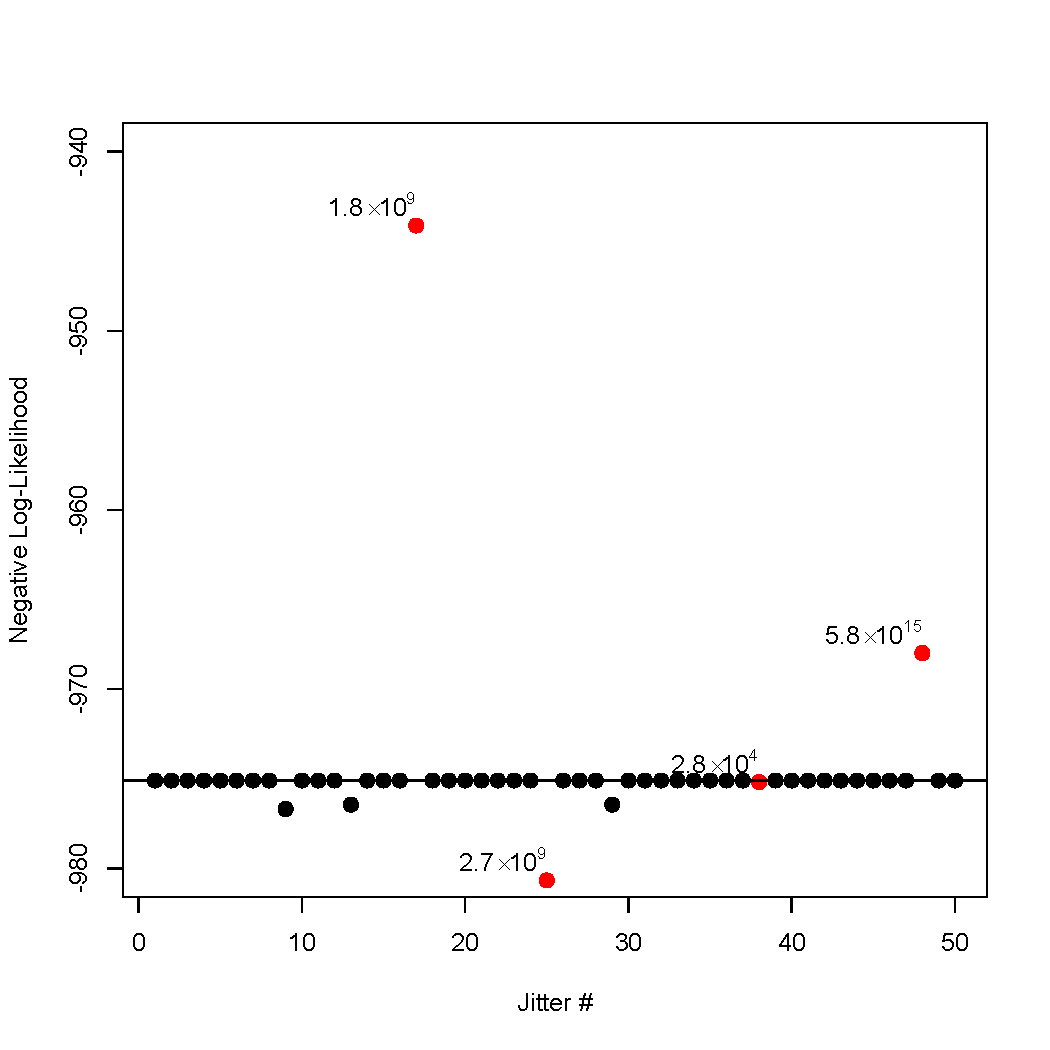
\includegraphics[width=1\linewidth]{fit_0_jitter_plt} 

}

\caption{Minimized negative log-likelihood for 50 fits where minimization used initial parameter values jittered from those provided by an initial fit for model $M_0$. Black jitters had maximum absolute gradient values < $10^{-2}$ and red jitters had values > 1.}\label{fig:jitter-M0}
\end{figure}
\pagebreak

\begin{figure}

{\centering 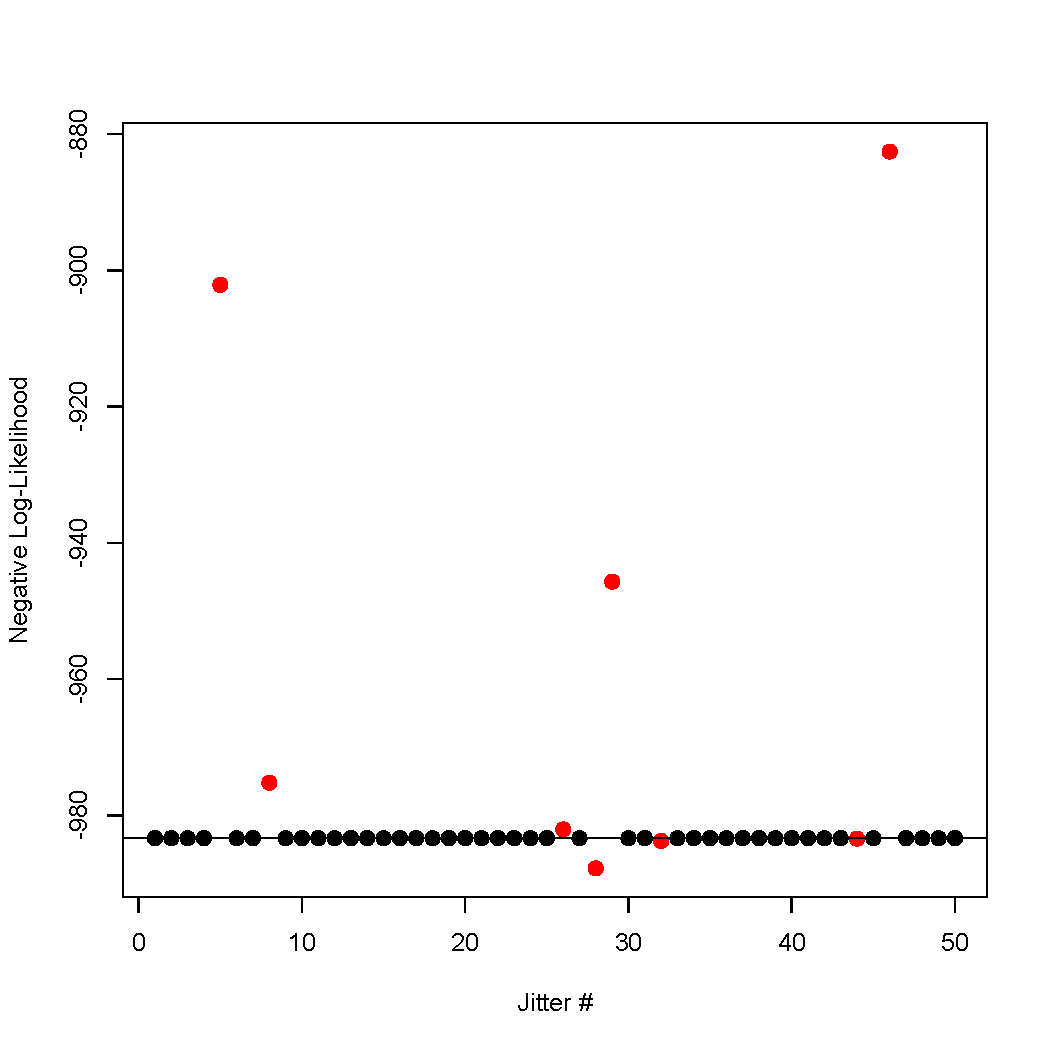
\includegraphics[width=1\linewidth]{fit_1_jitter_plt} 

}

\caption{Minimized negative log-likelihood for 50 fits where minimization used initial parameter values jittered from those provided by an initial fit for model $M_1$. Fits with black dots had maximum absolute gradient value < 0.01 and fits with red dots had values > 10.}\label{fig:jitter-M1}
\end{figure}
\pagebreak

\begin{figure}

{\centering 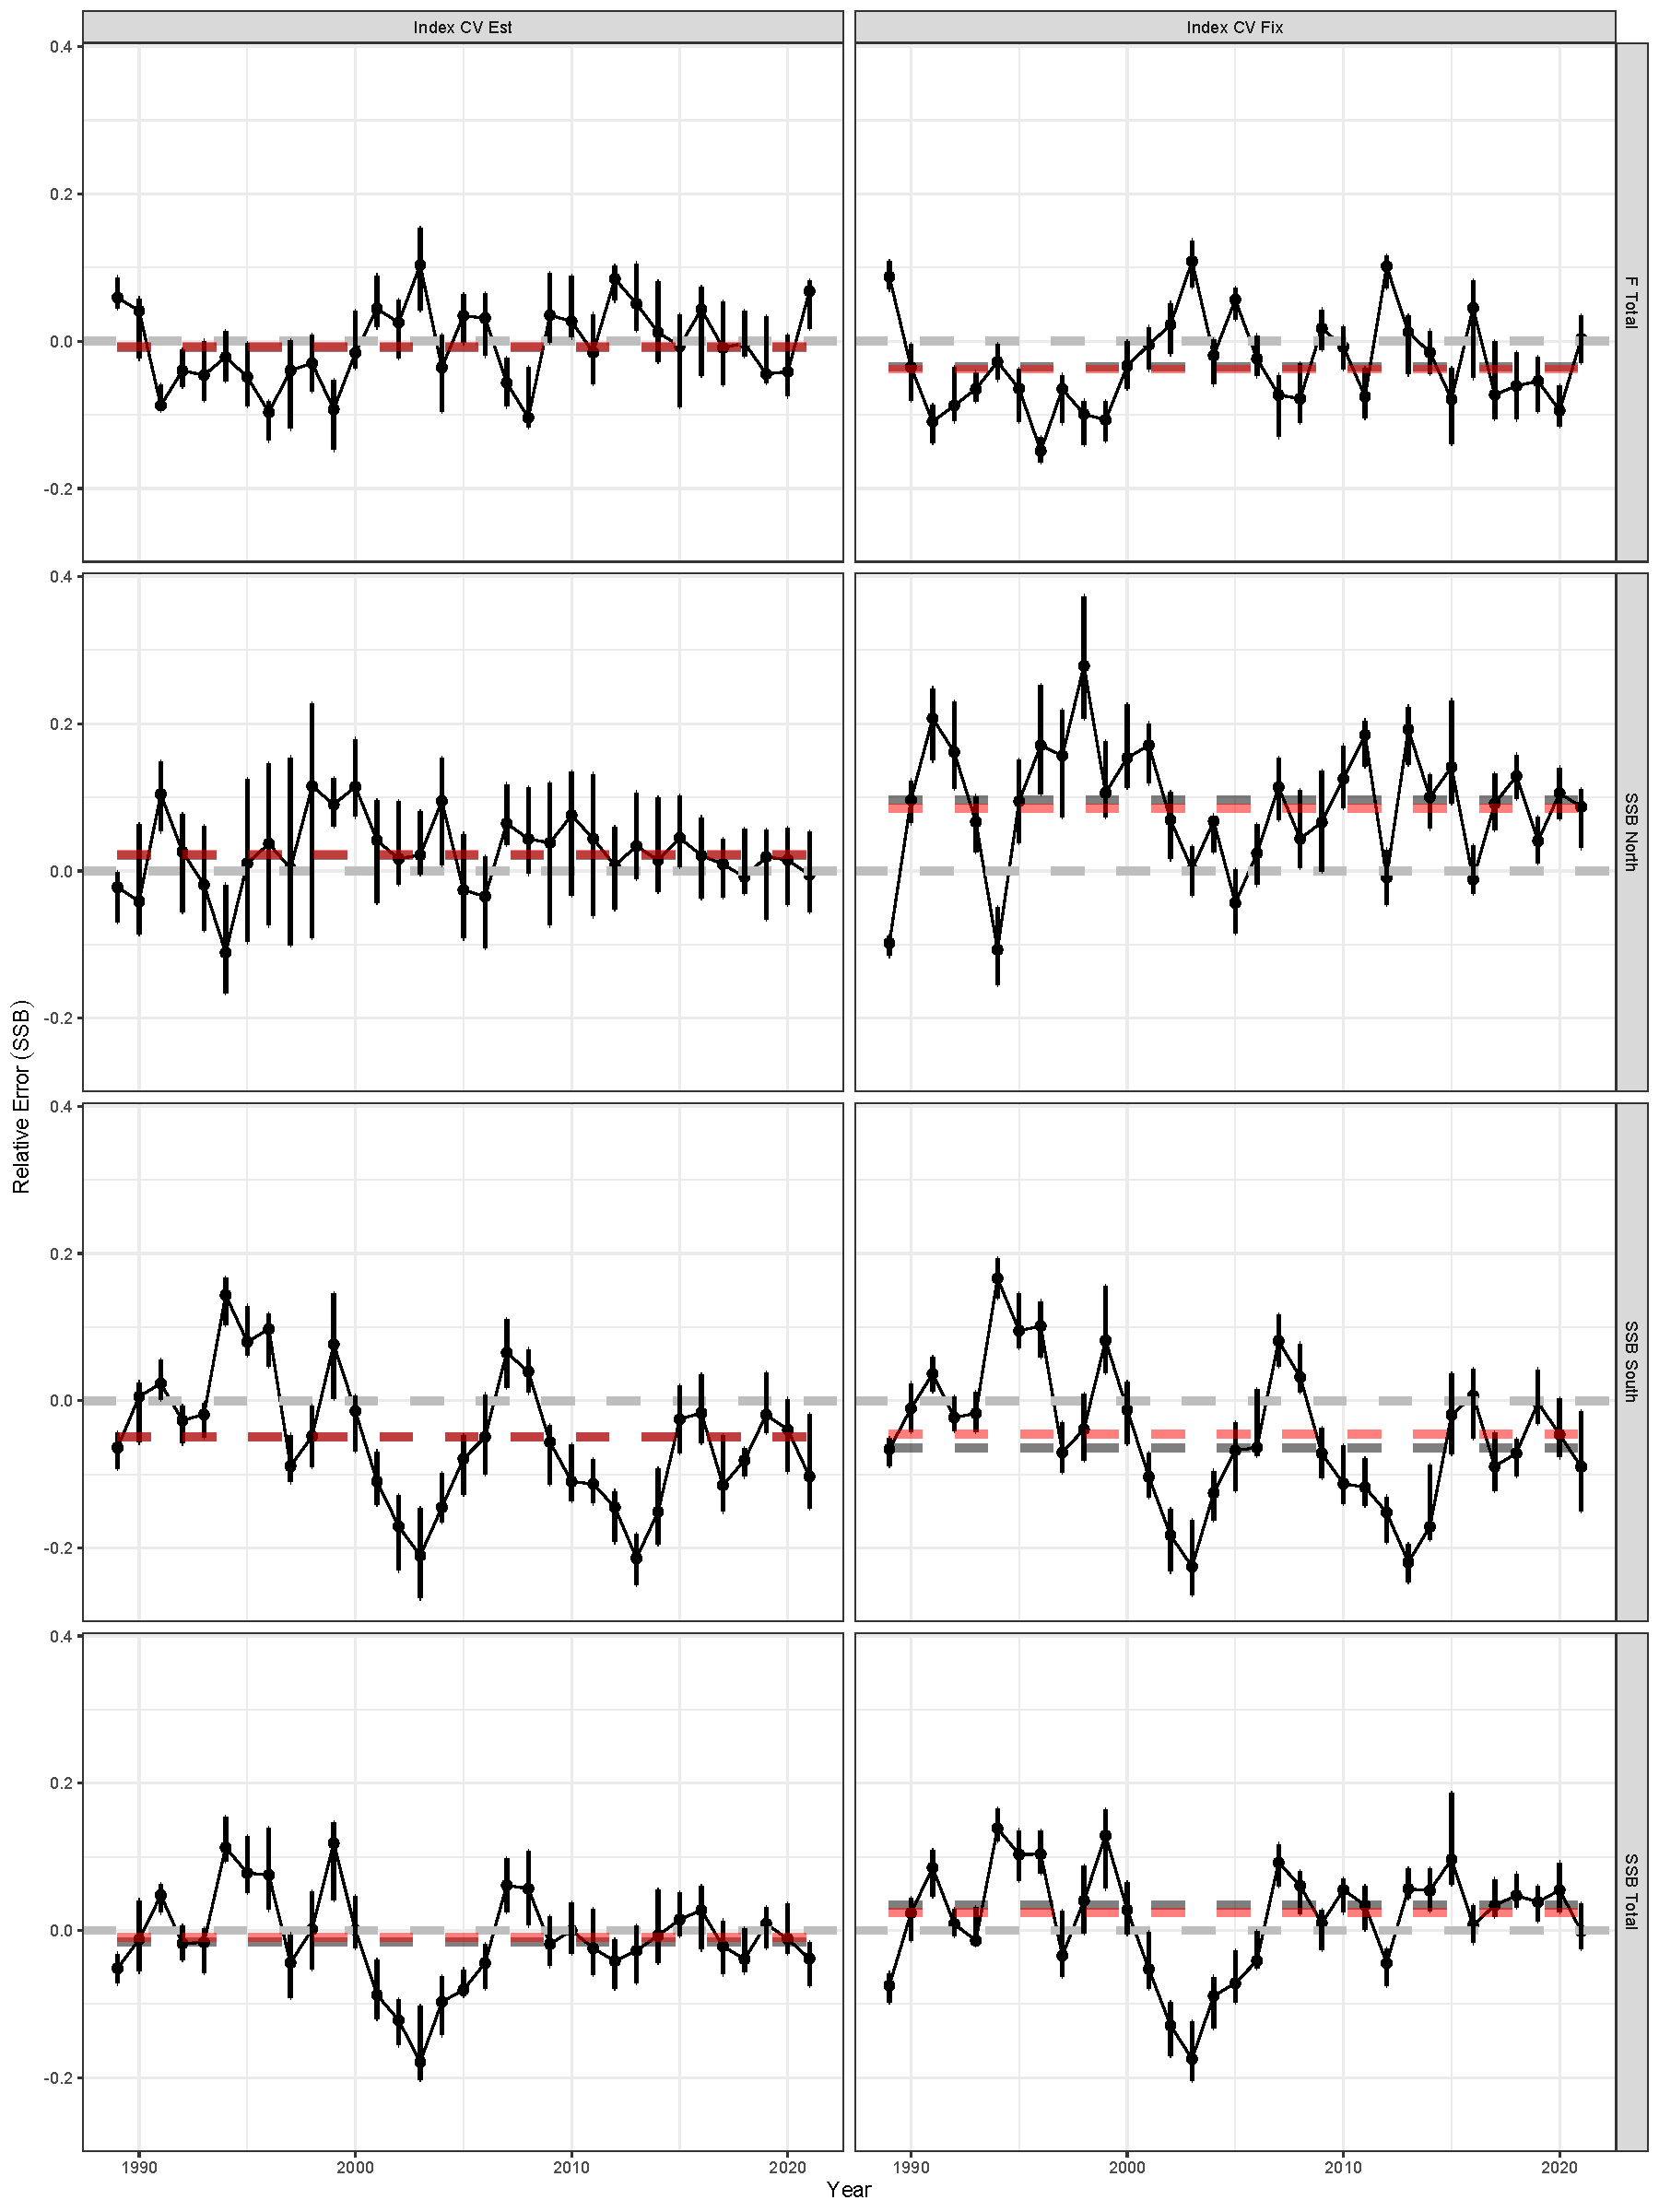
\includegraphics[width=1\linewidth]{self_test_results} 

}

\caption{Median relative error of SSB (Total and by stock component) and total fully-selected fishing mortality for estimation models fitted to simulated data from model $M_1$ where the observation variance of log-indices are fixed and estimated. Black and Red dashed lines represent the median of the annual medians and the median across all annual relative errors, respectively. Vertical lines represent 95\% confidence intervals.}\label{fig:self-test-fig}
\end{figure}

\begin{landscape}

\begin{figure}

{\centering 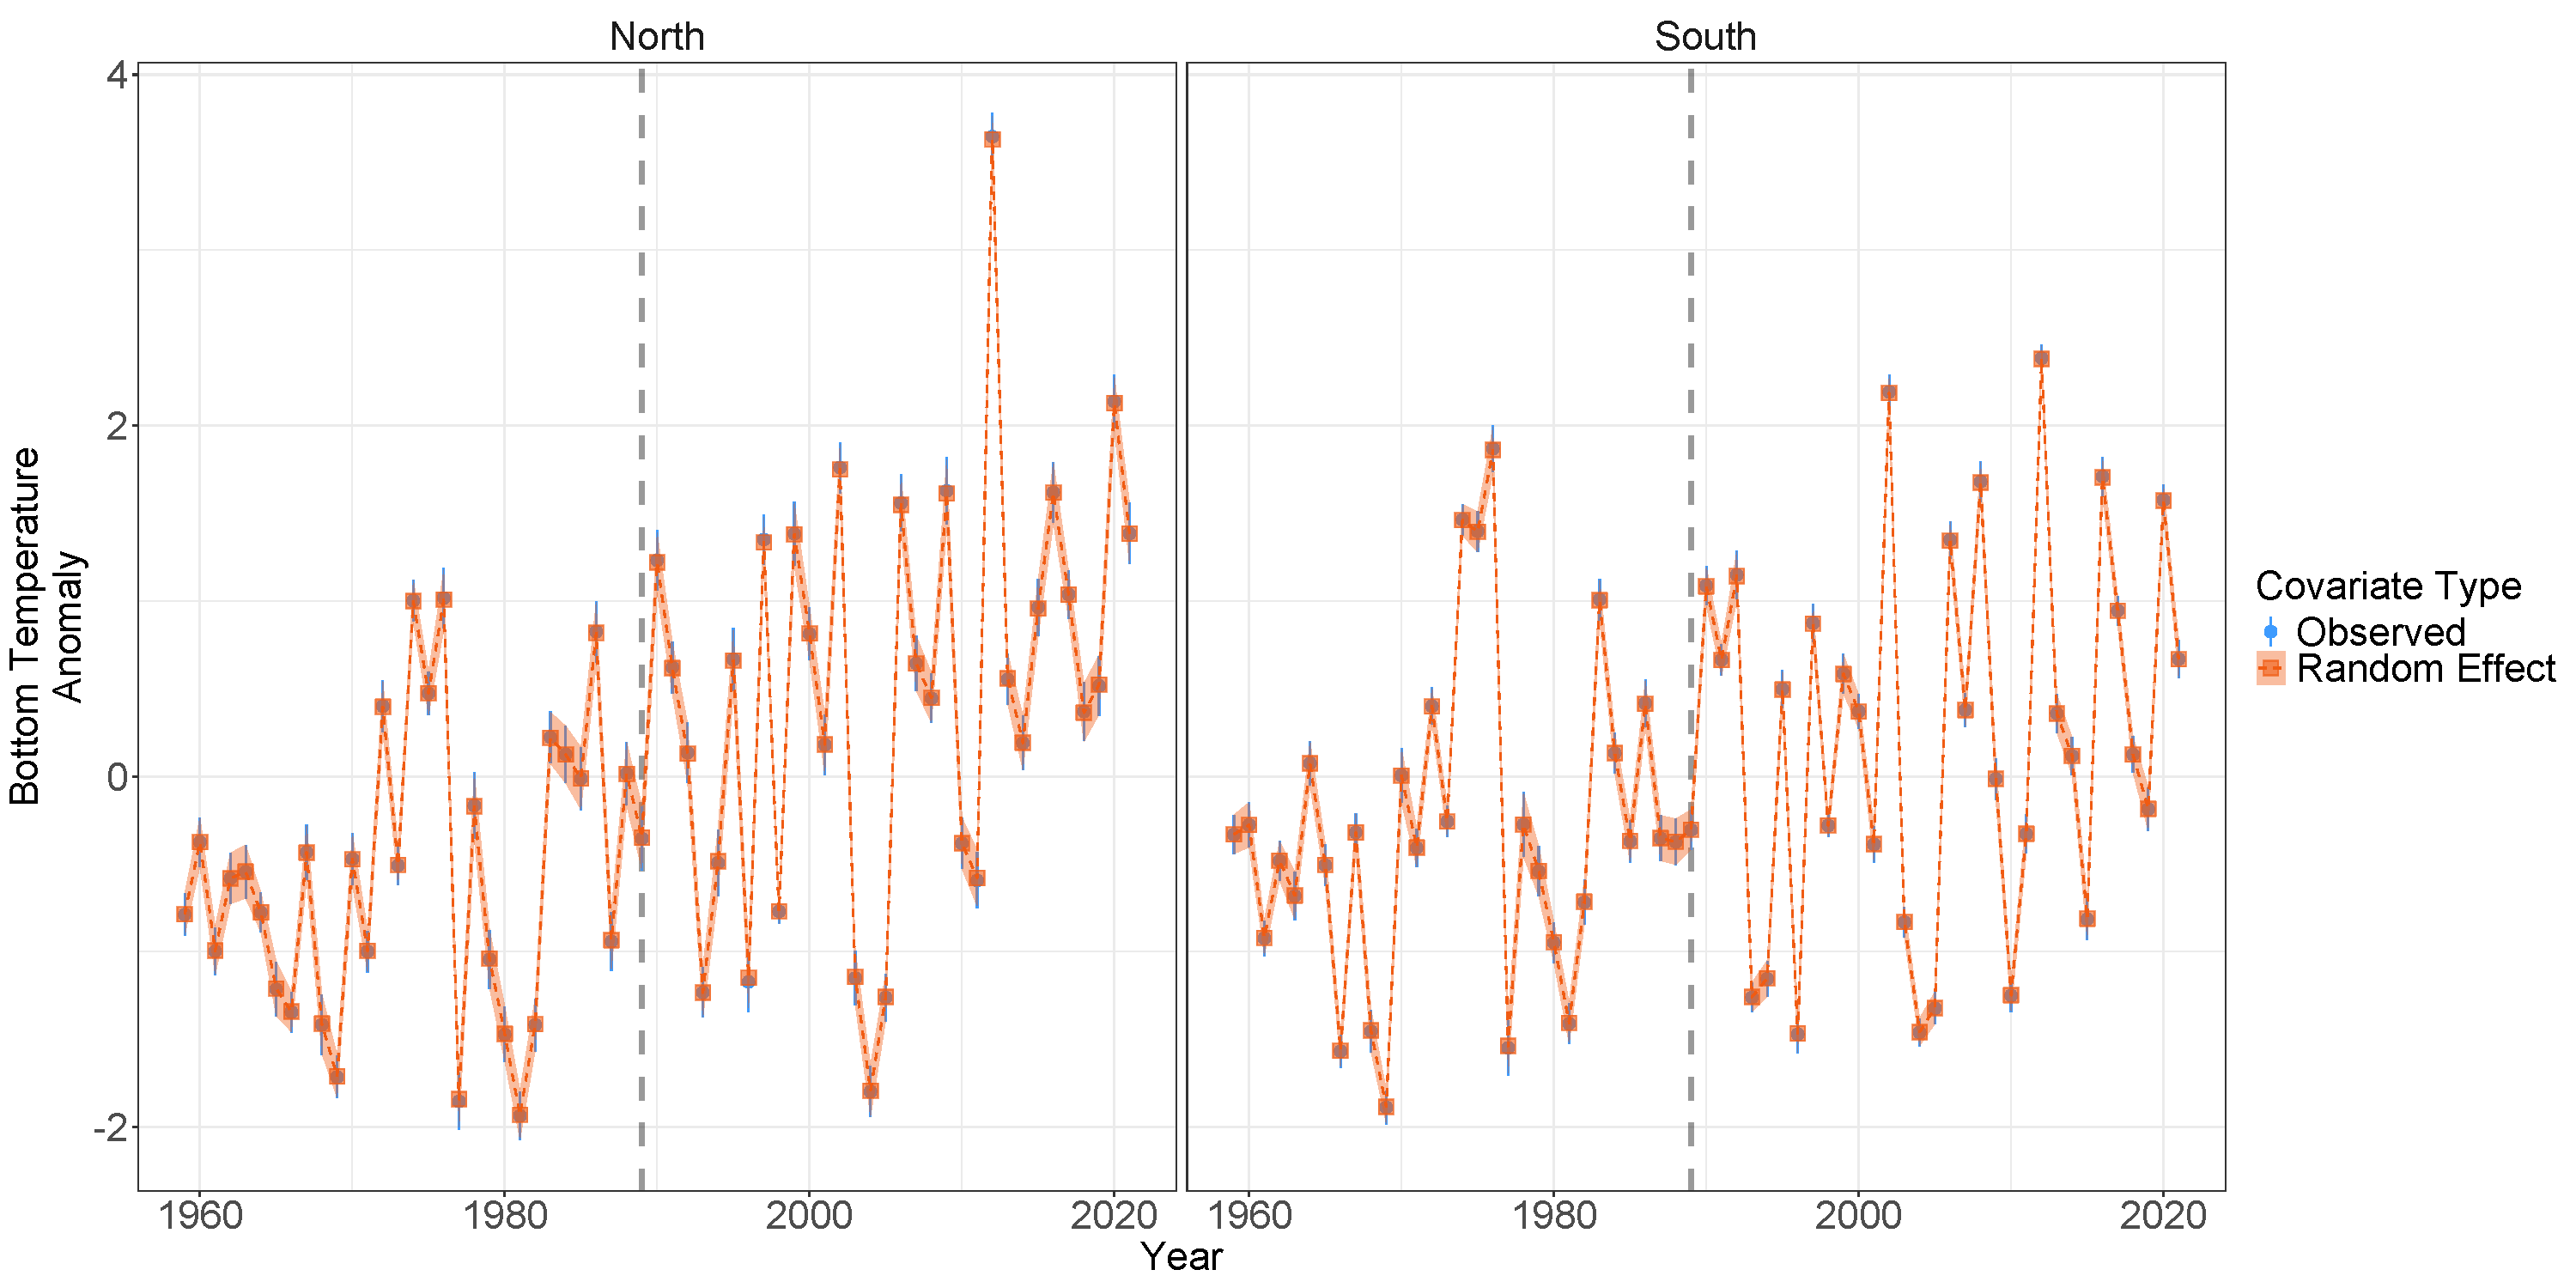
\includegraphics[width=1\linewidth]{BTA_full_fig} 

}

\caption{Observations with 95\% confidence intervals (points with vertical lines) and posterior estimates with 95\% confidence intervals (lines with polygons) of bottom temperature anomalies in the north and south regions from model $M_1$. Gray vertical line defines the first year that the black sea bass stock is modeled.}\label{fig:bottom-temperature}
\end{figure}

\end{landscape}
\pagebreak

\begin{figure}

{\centering 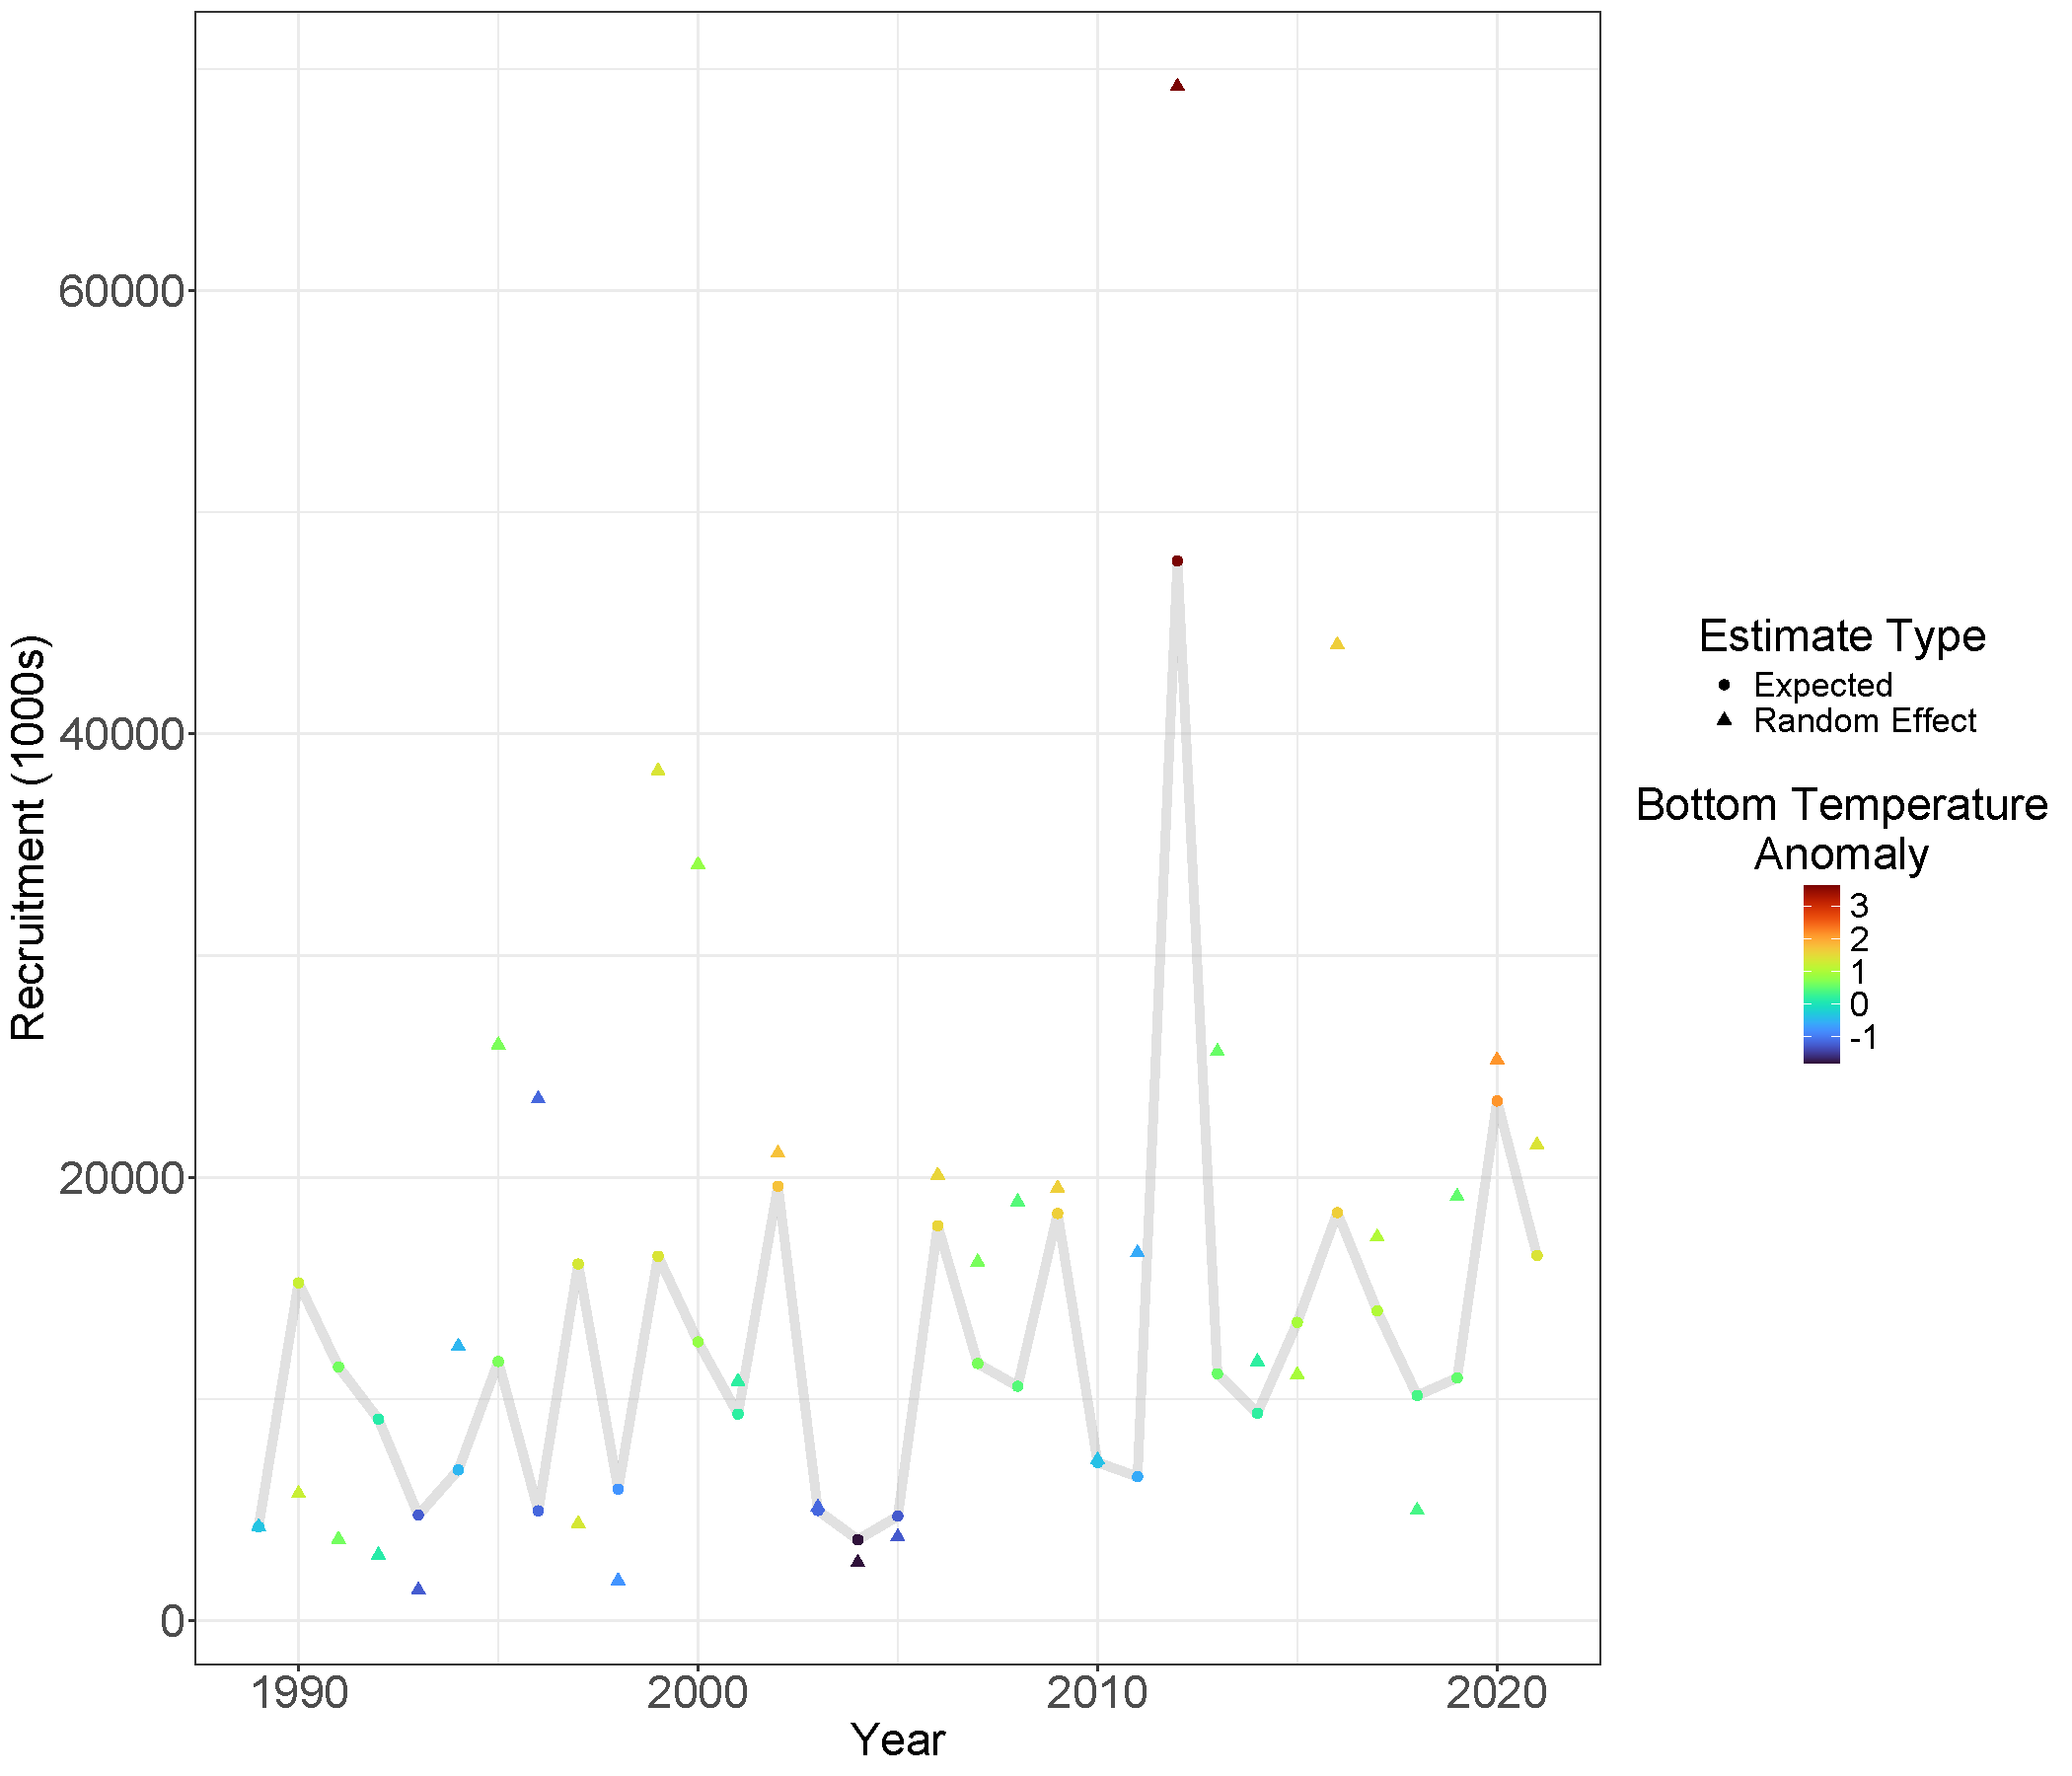
\includegraphics[width=1\linewidth]{best_R_Ecov} 

}

\caption{Expected and random effect recruitment estimates for the northern stock component. Color of points defined by the corresponding annual bottom temperature anomaly.}\label{fig:BT-Ecov-R}
\end{figure}
\pagebreak

\begin{figure}

{\centering 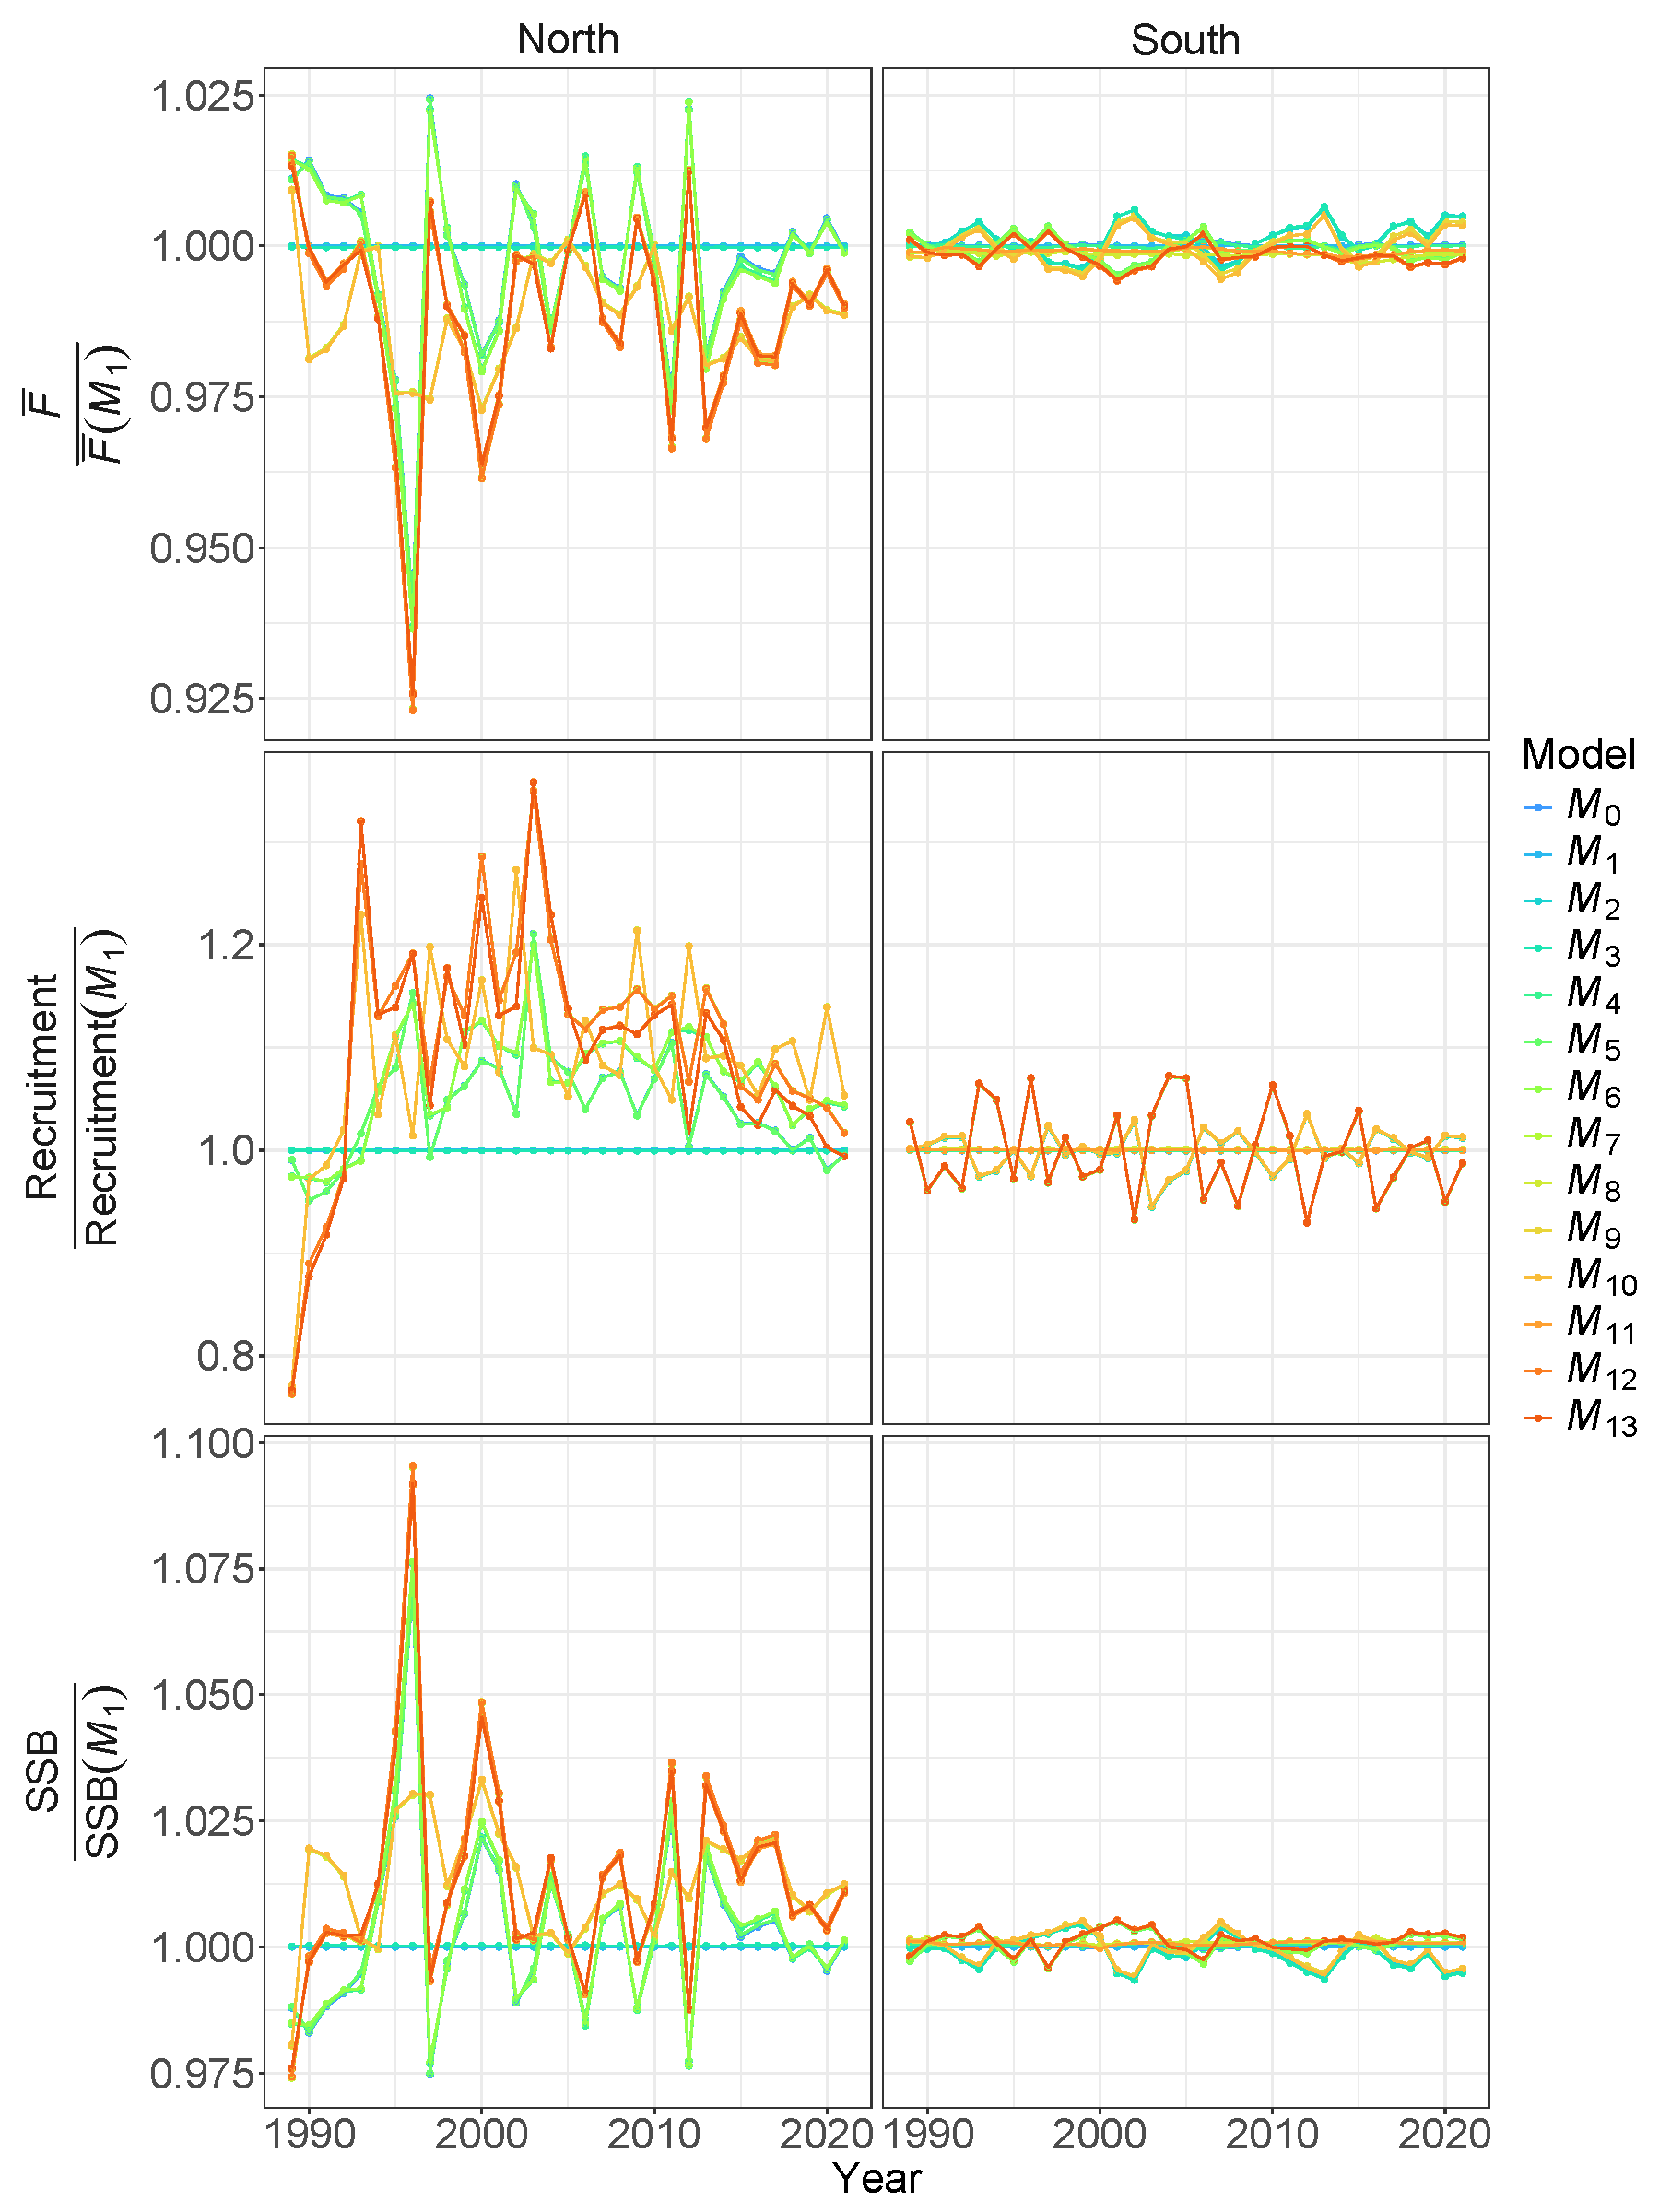
\includegraphics[height=0.95\textheight]{SSB_F_R_rel_M1} 

}

\caption{Estimates of SSB, F, and recruitment relative to those of the best performing model, $M_1$.}\label{fig:SSB-F-R-rel-M1}
\end{figure}

\begin{figure}

{\centering 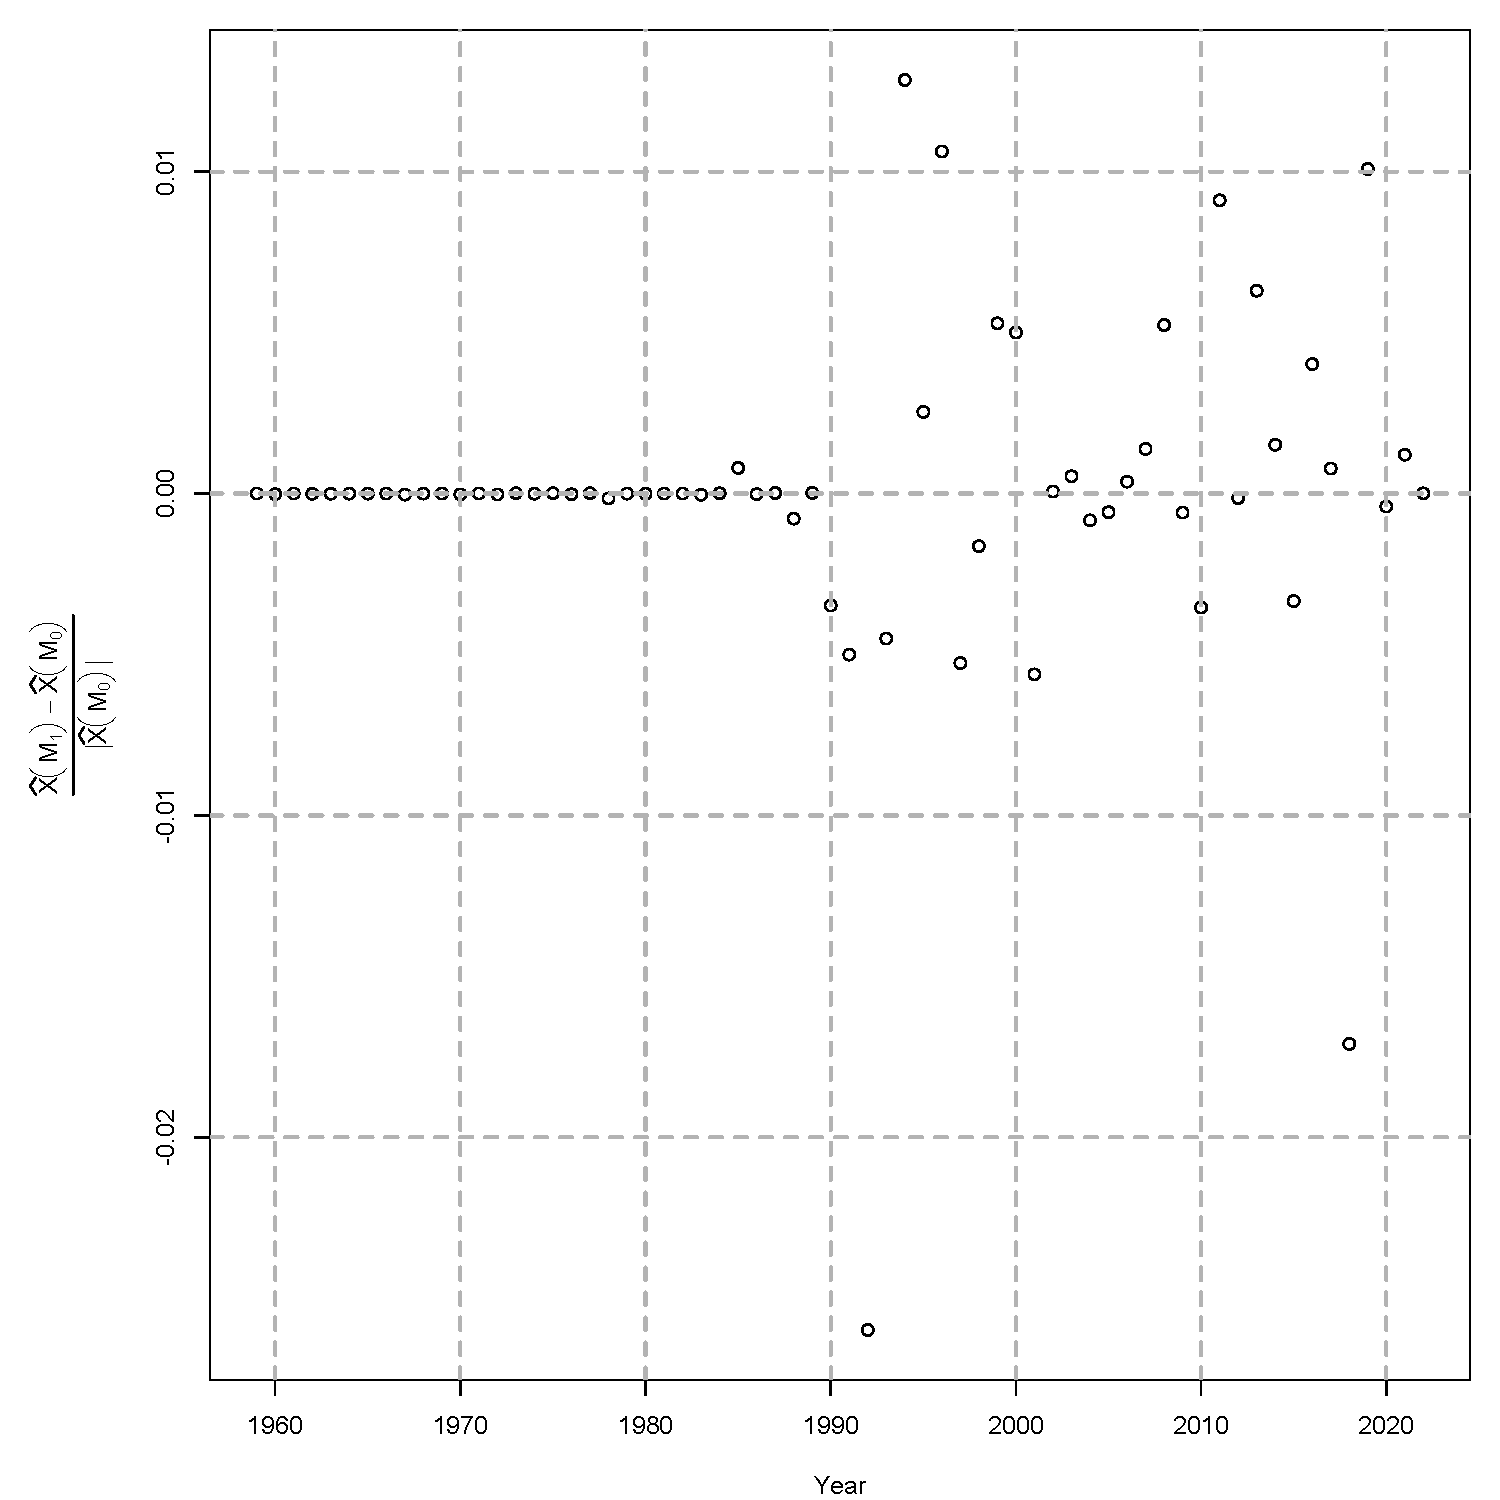
\includegraphics[height=0.95\textheight]{Ecov_M1_rel_M0} 

}

\caption{Relative differences in posterior estimates of northern region bottom temperature anomalies ($\widehat X$) from the null model without effects on recruitment ($M_0$) and with effects on the northern stock component ($M_1$).}\label{fig:Ecov-M1-rel-M0}
\end{figure}

\begin{figure}

{\centering 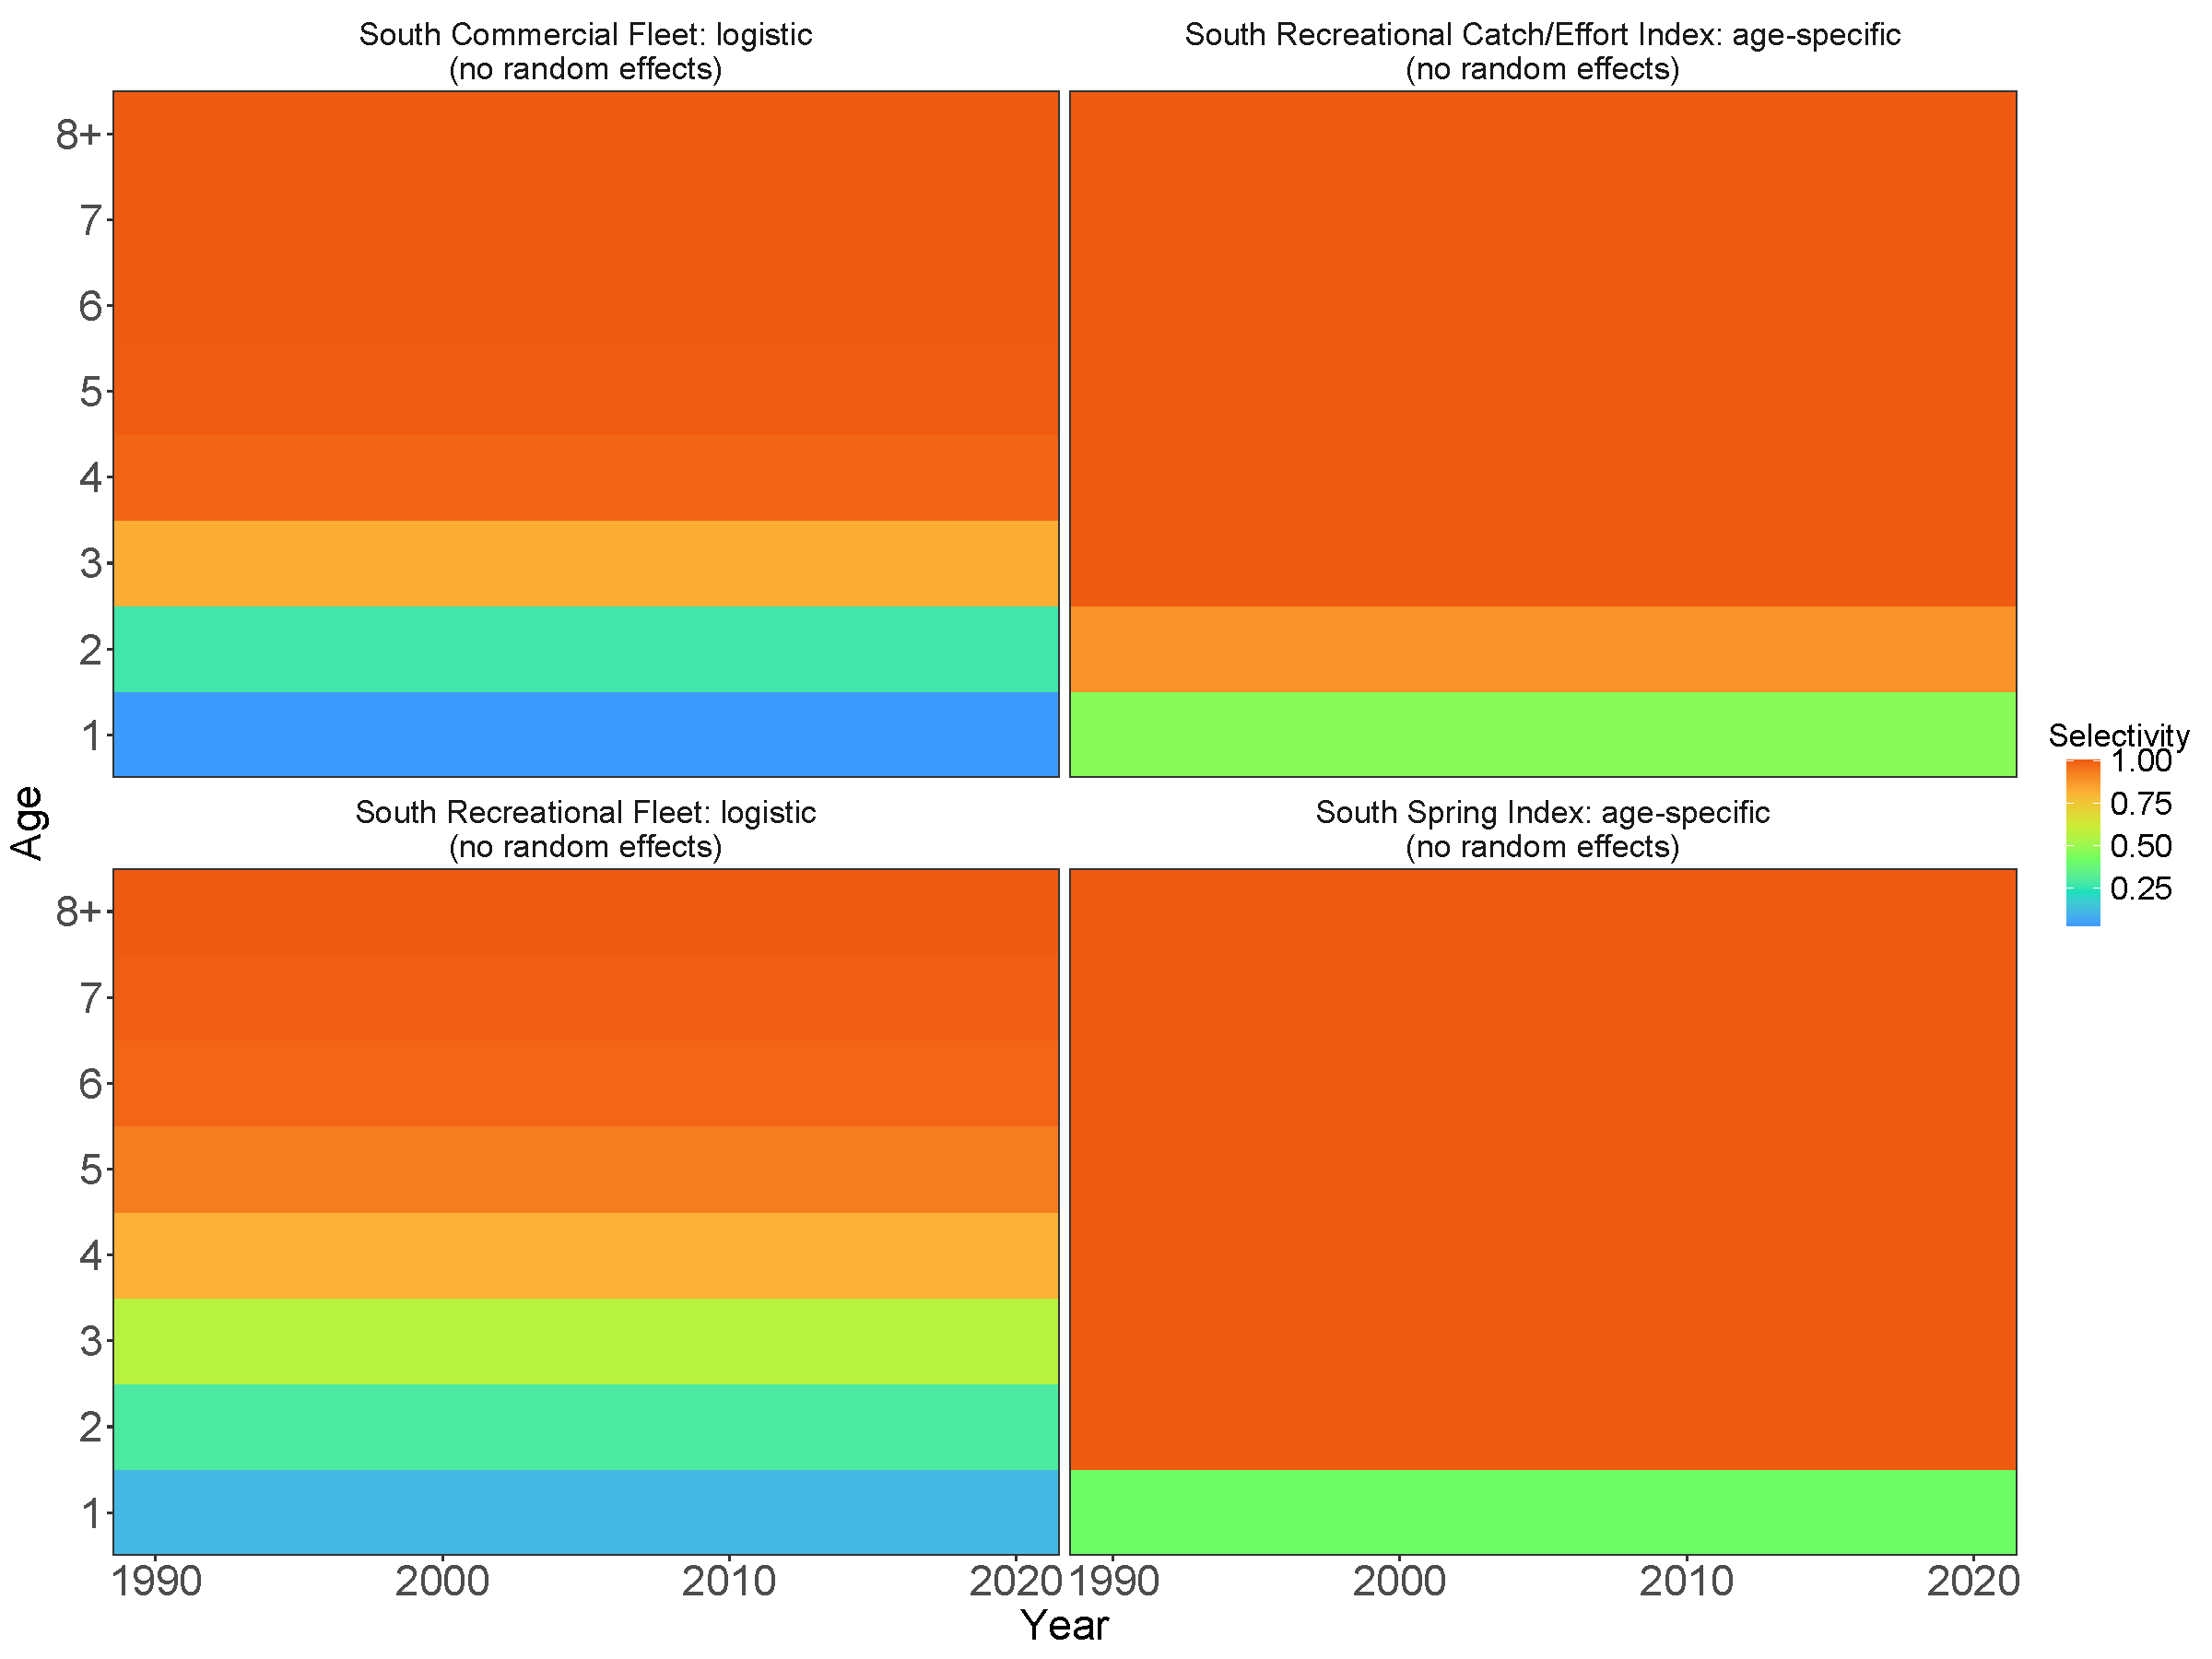
\includegraphics[height=0.95\textheight]{selectivity_south_plot} 

}

\caption{Selectivty for fleets and indices in the southern region.}\label{fig:selectivity-south}
\end{figure}
\pagebreak

\begin{landscape}

\begin{figure}

{\centering 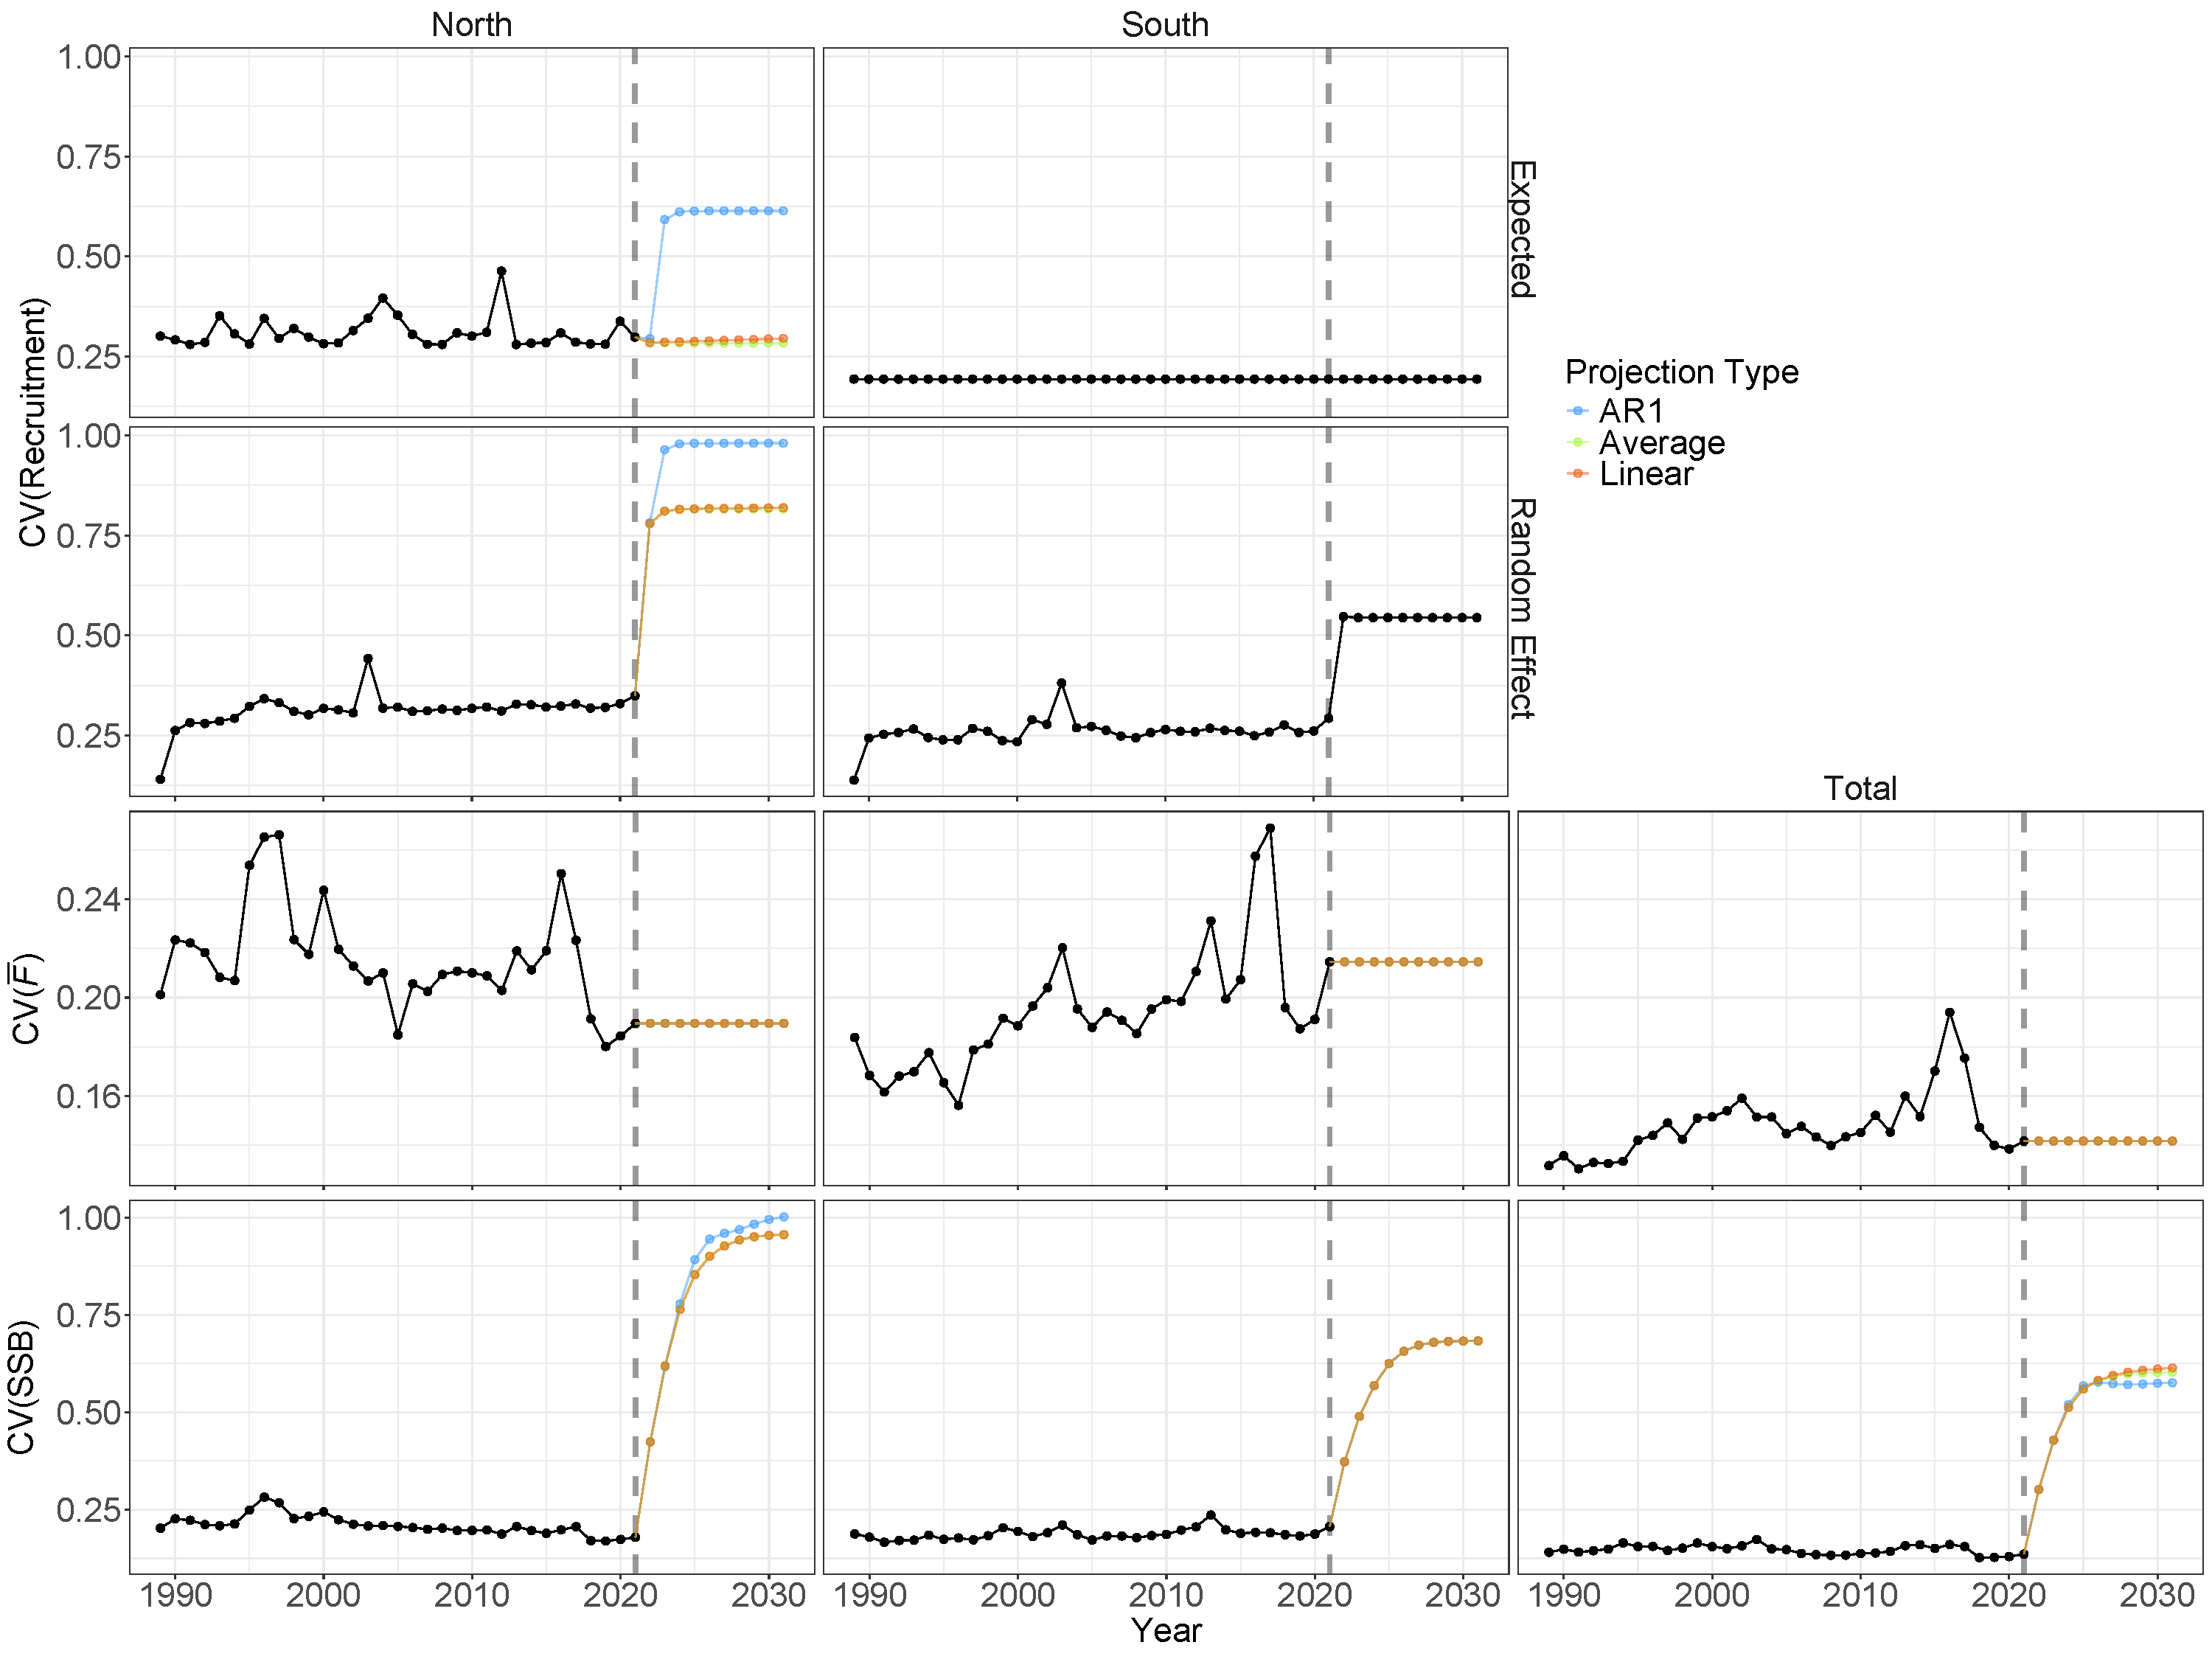
\includegraphics[height=0.9\textheight]{R_SSB_F_cv_results} 

}

\caption{Coefficients of variation for estimates of alternative recruitment estimates (random effects or expected), average fishing mortality at age 6 and 7, and SSB by region and in total from model $M_1$. Values in years after 2021 are from projecting model $M_1$ under three alternative assumptions for the bottom temperature anomolies. \DIFaddbeginFL \DIFaddFL{Vertical dotted lines indicate the last year of data.}\DIFaddendFL }\label{fig:R-F-SSB-CVs}
\end{figure}
\end{landscape}

\begin{figure}

{\centering 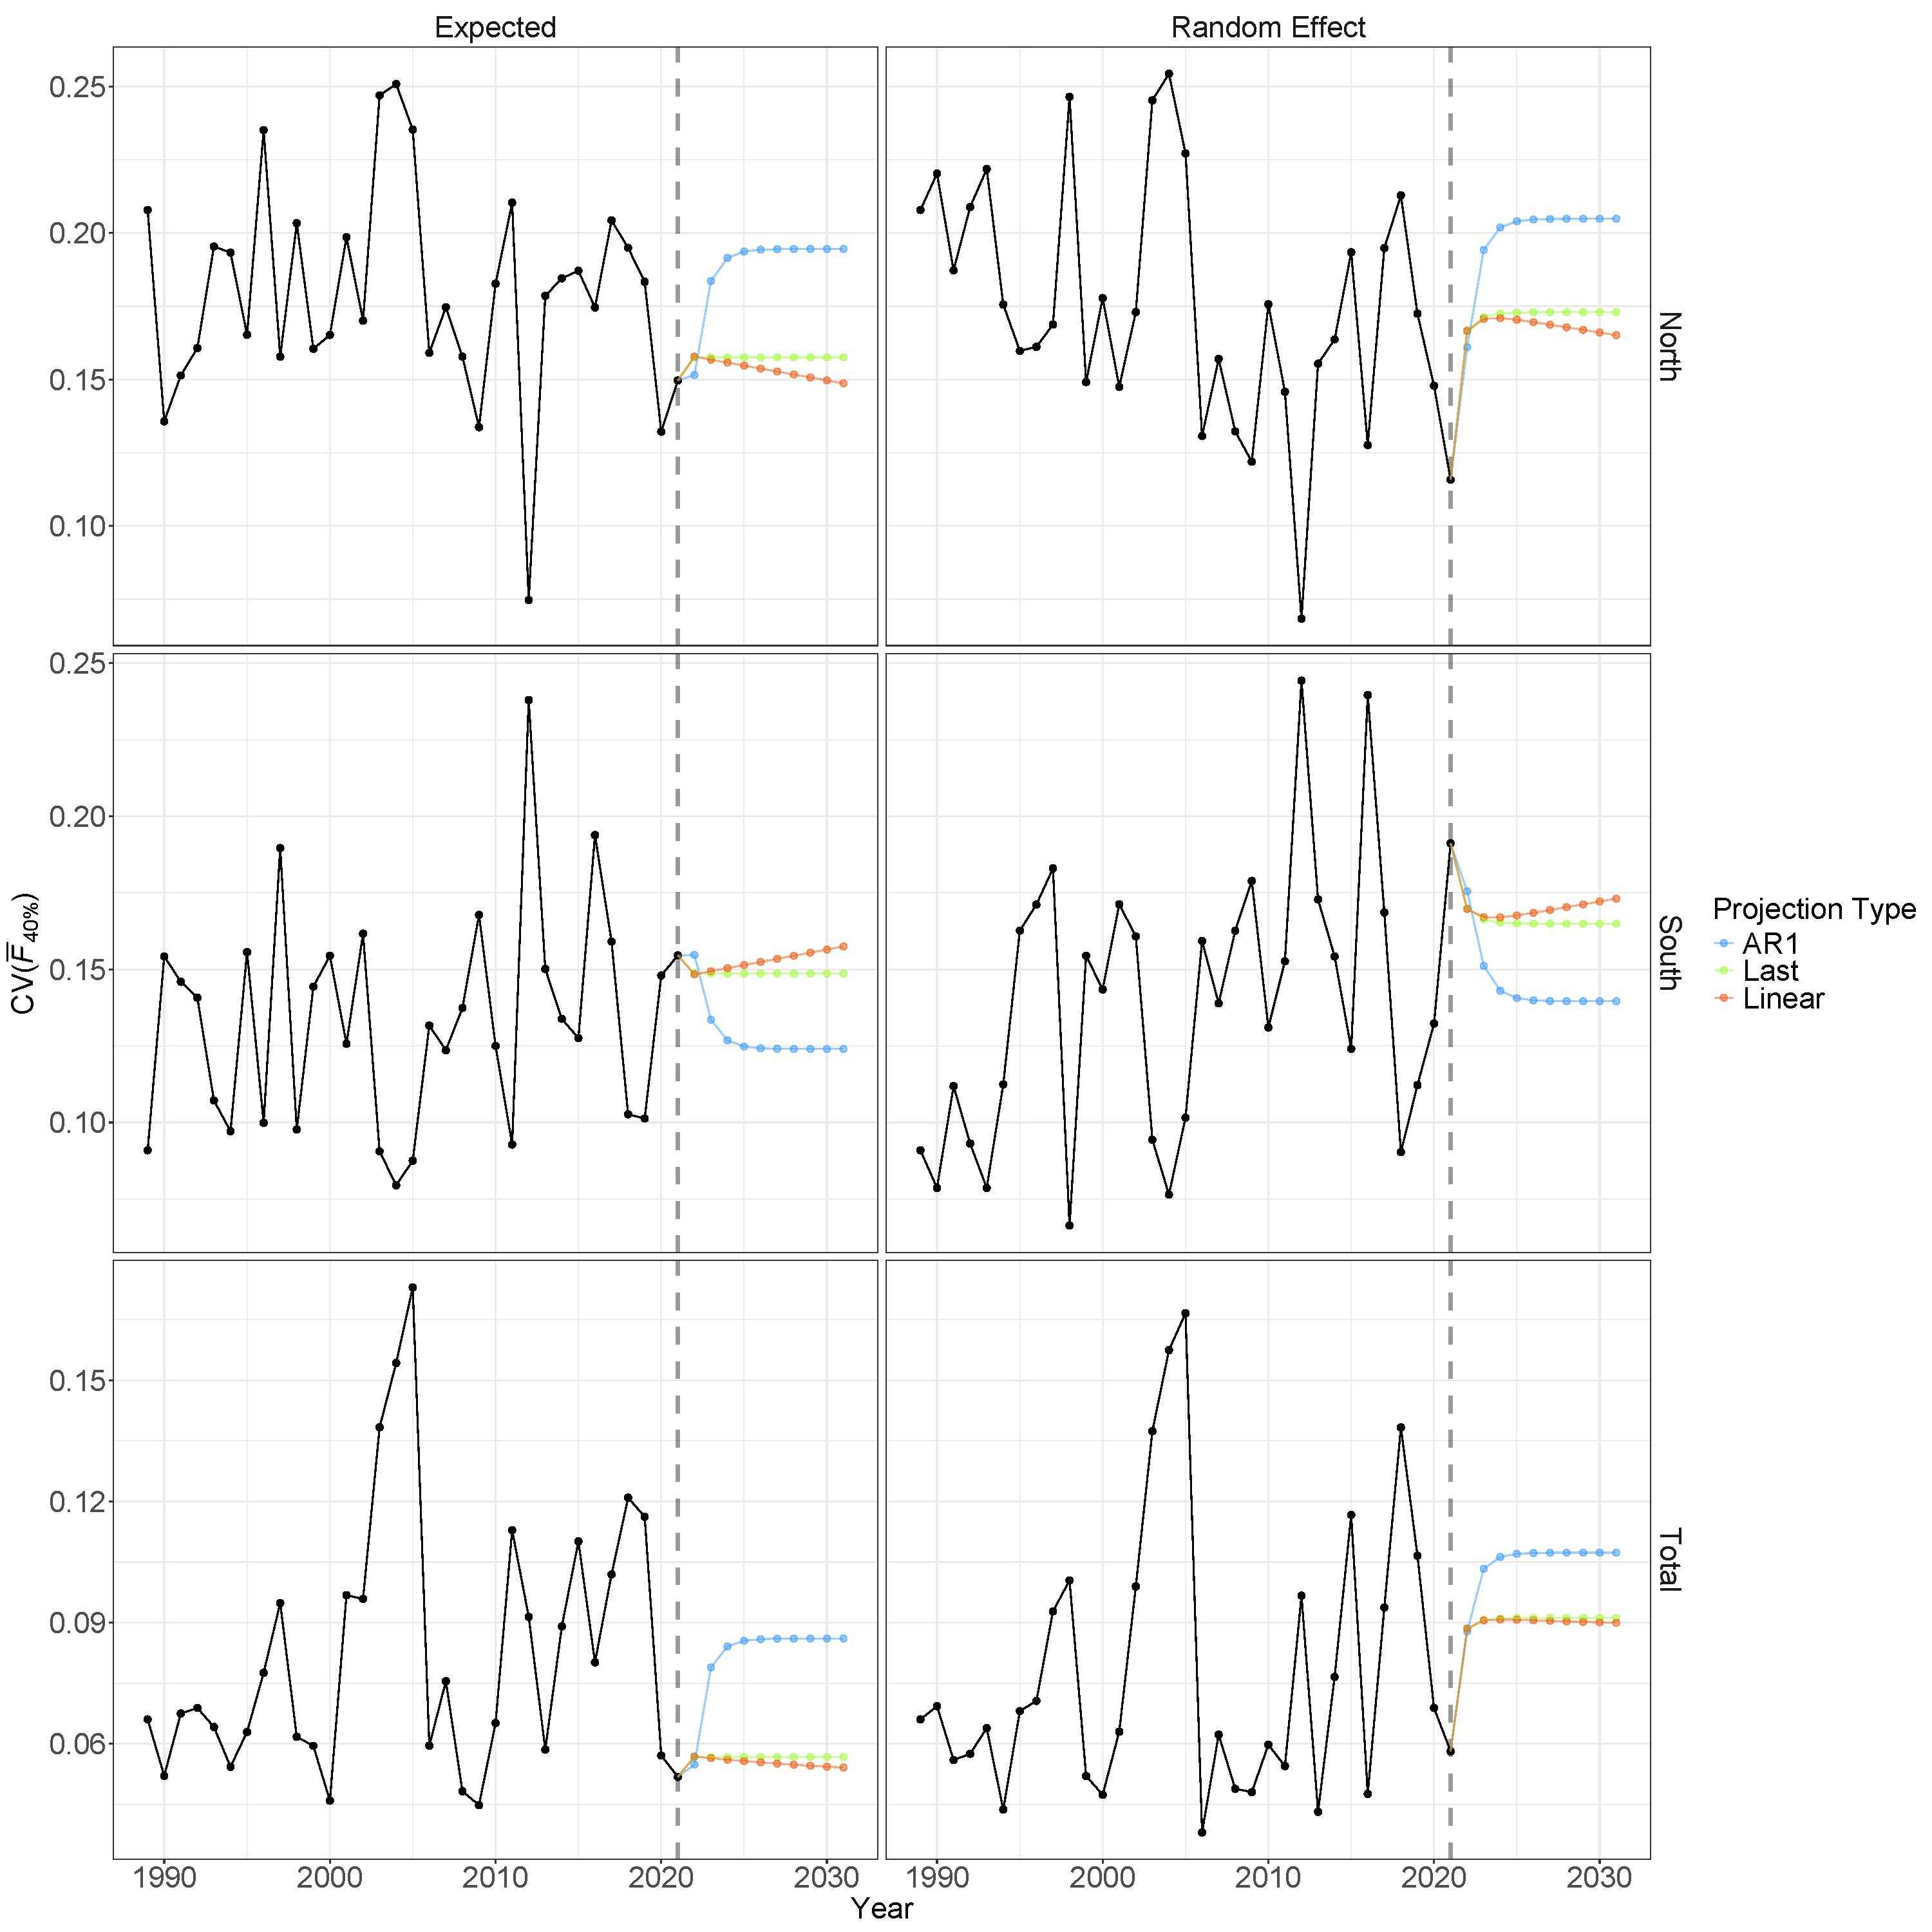
\includegraphics[height=0.95\textheight]{proj_F40_CV} 

}

\caption{Coefficients of variation for annual equilibrium average $F$ at ages 6 and 7 that produces the 40\% spawning potential ratio as a function of annual expected recruitment or recruitment random effects and annual inputs to $\upphi(\widetilde{F})$ calculations. Estimates in years after 2021 are from projecting model $M_1$ under three alternative assumptions for the bottom temperature anomolies. \DIFaddbeginFL \DIFaddFL{Vertical dotted lines indicate the last year of data.}\DIFaddendFL }\label{fig:annual-F40-cvs}
\end{figure}

\begin{figure}

{\centering 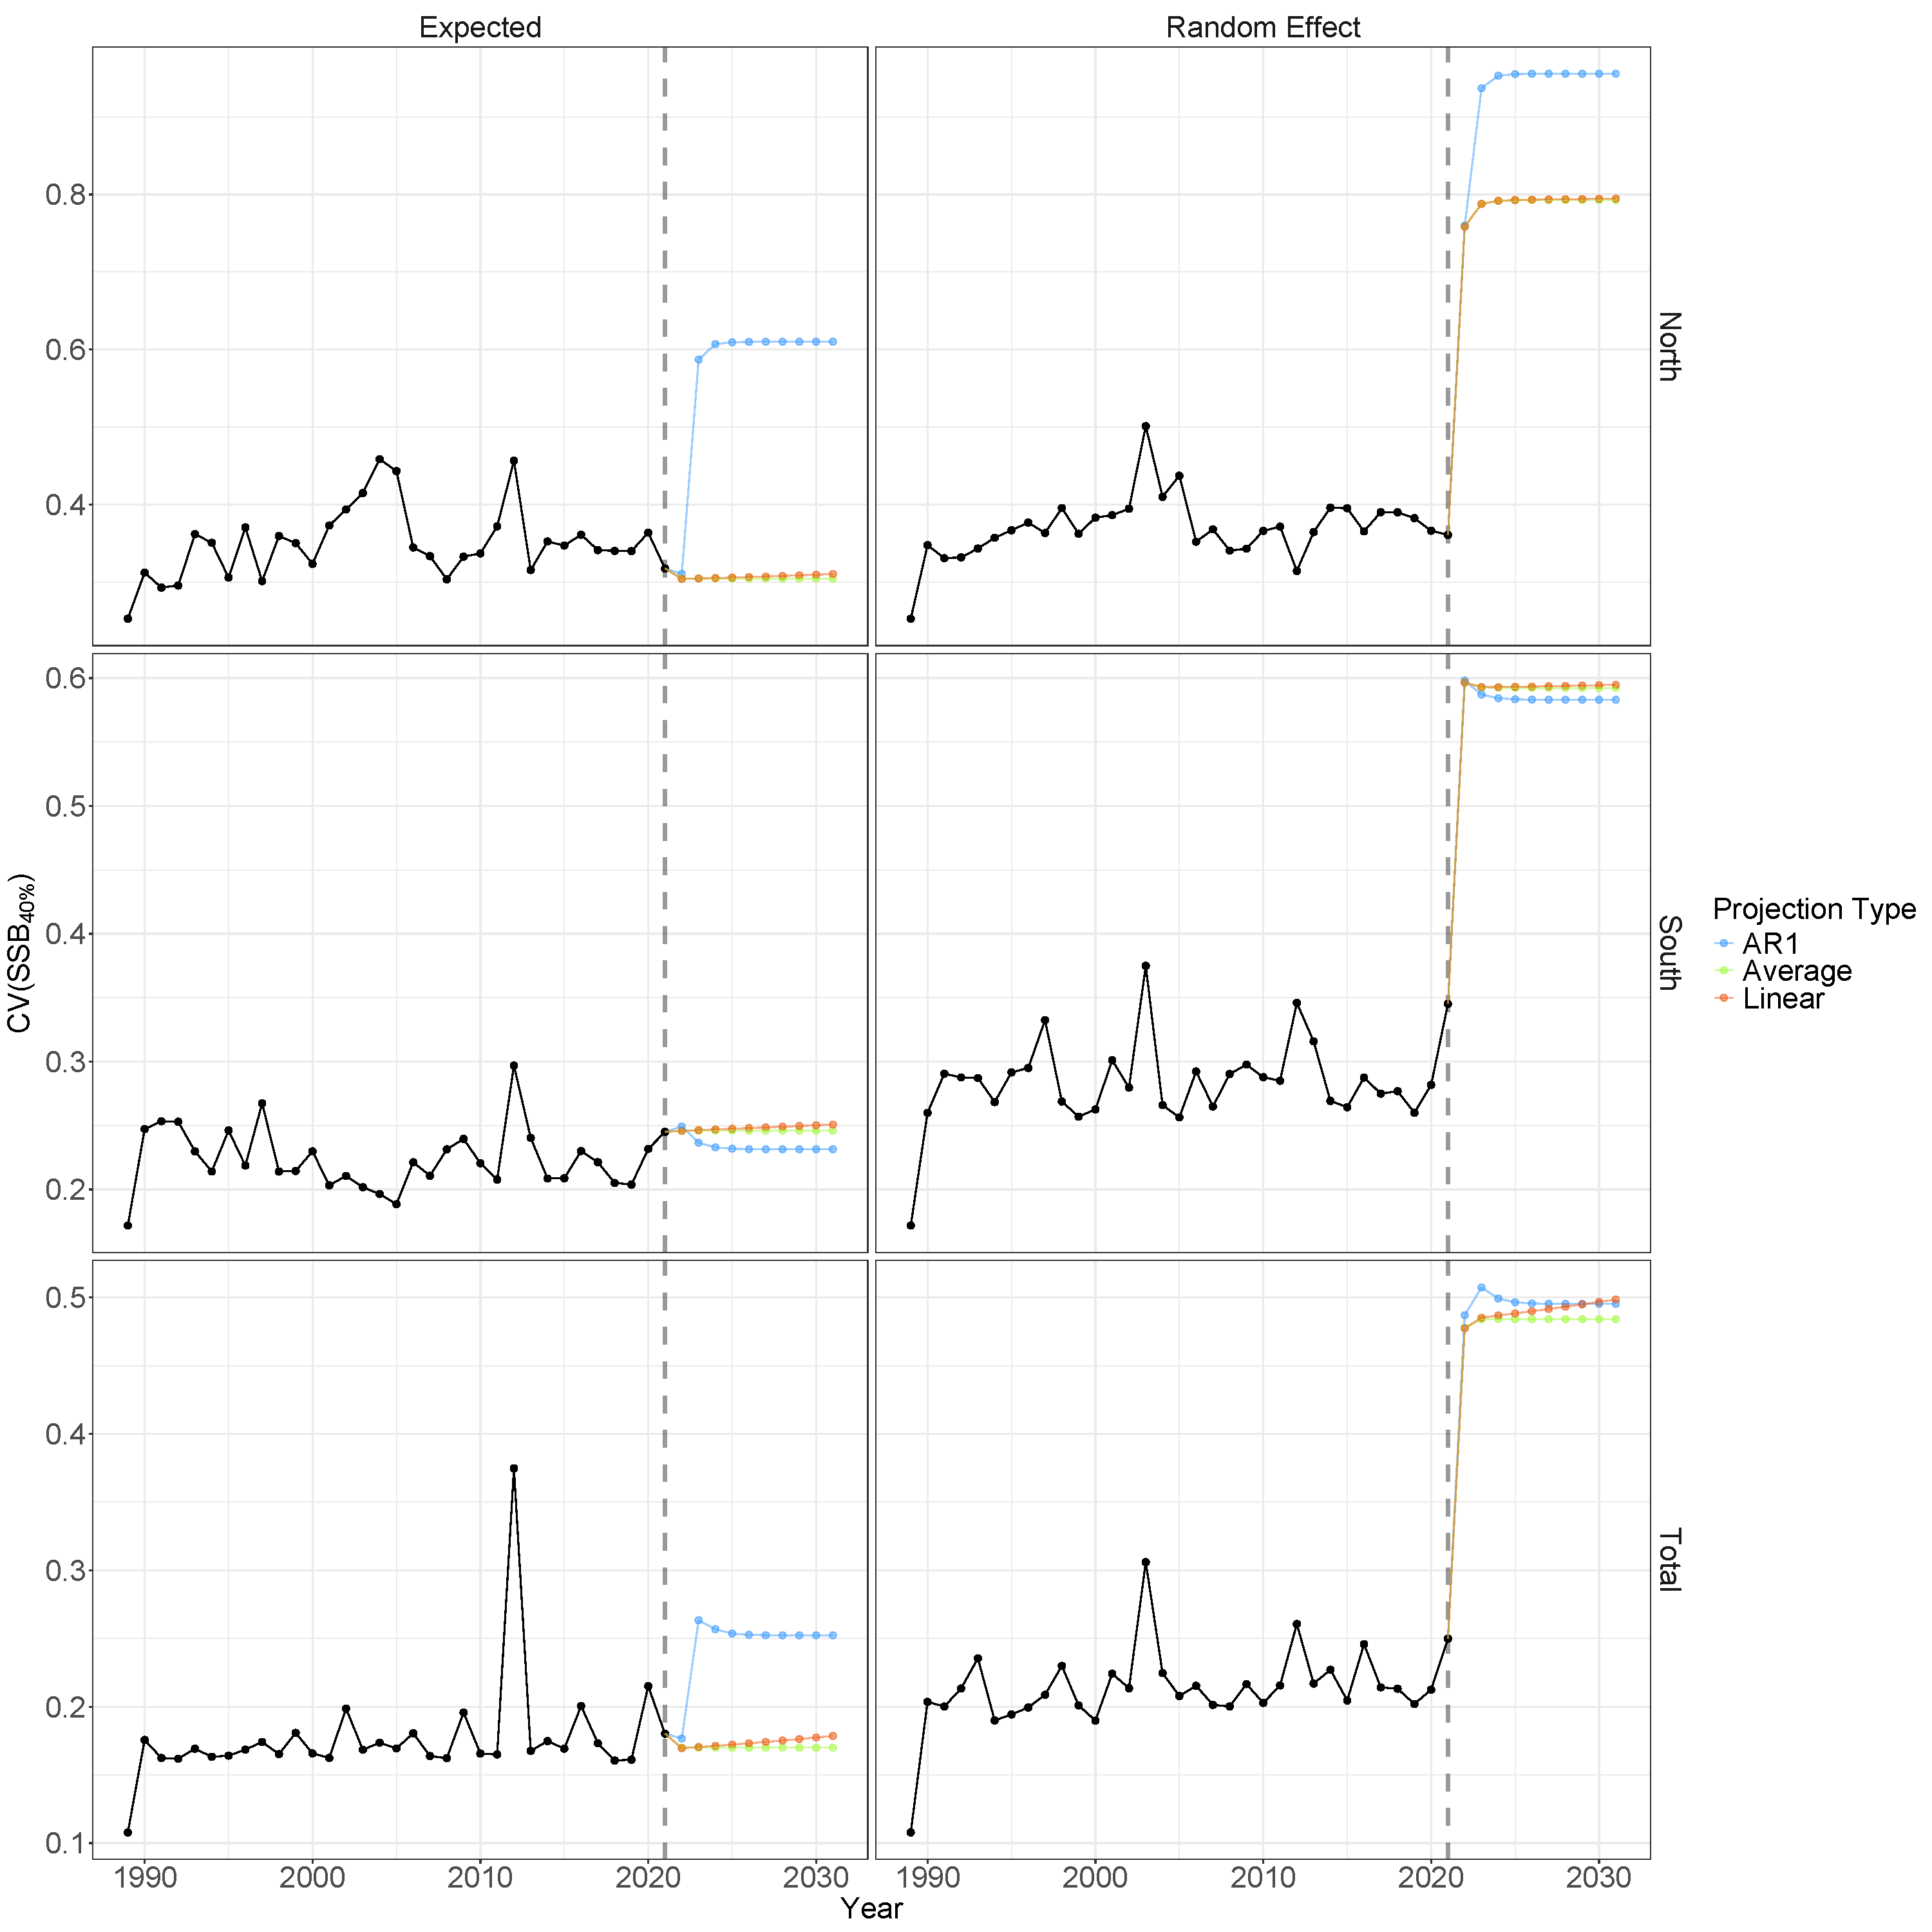
\includegraphics[height=0.95\textheight]{proj_SSB40_CV} 

}

\caption{Coefficients of variation for annual equilibrium SSB$_{40\%}$ as a function of annual expected recruitment or recruitment random effects and annual inputs to $\upphi(\widetilde{F})$ calculations and alternative annual recruitment types. Estimates in years after 2021 are from projecting model $M_1$ under three alternative assumptions for the bottom temperature anomolies. \DIFaddbeginFL \DIFaddFL{Vertical dotted lines indicate the last year of data.}\DIFaddendFL }\label{fig:annual-SSB40-cvs}
\end{figure}

\begin{figure}

{\centering 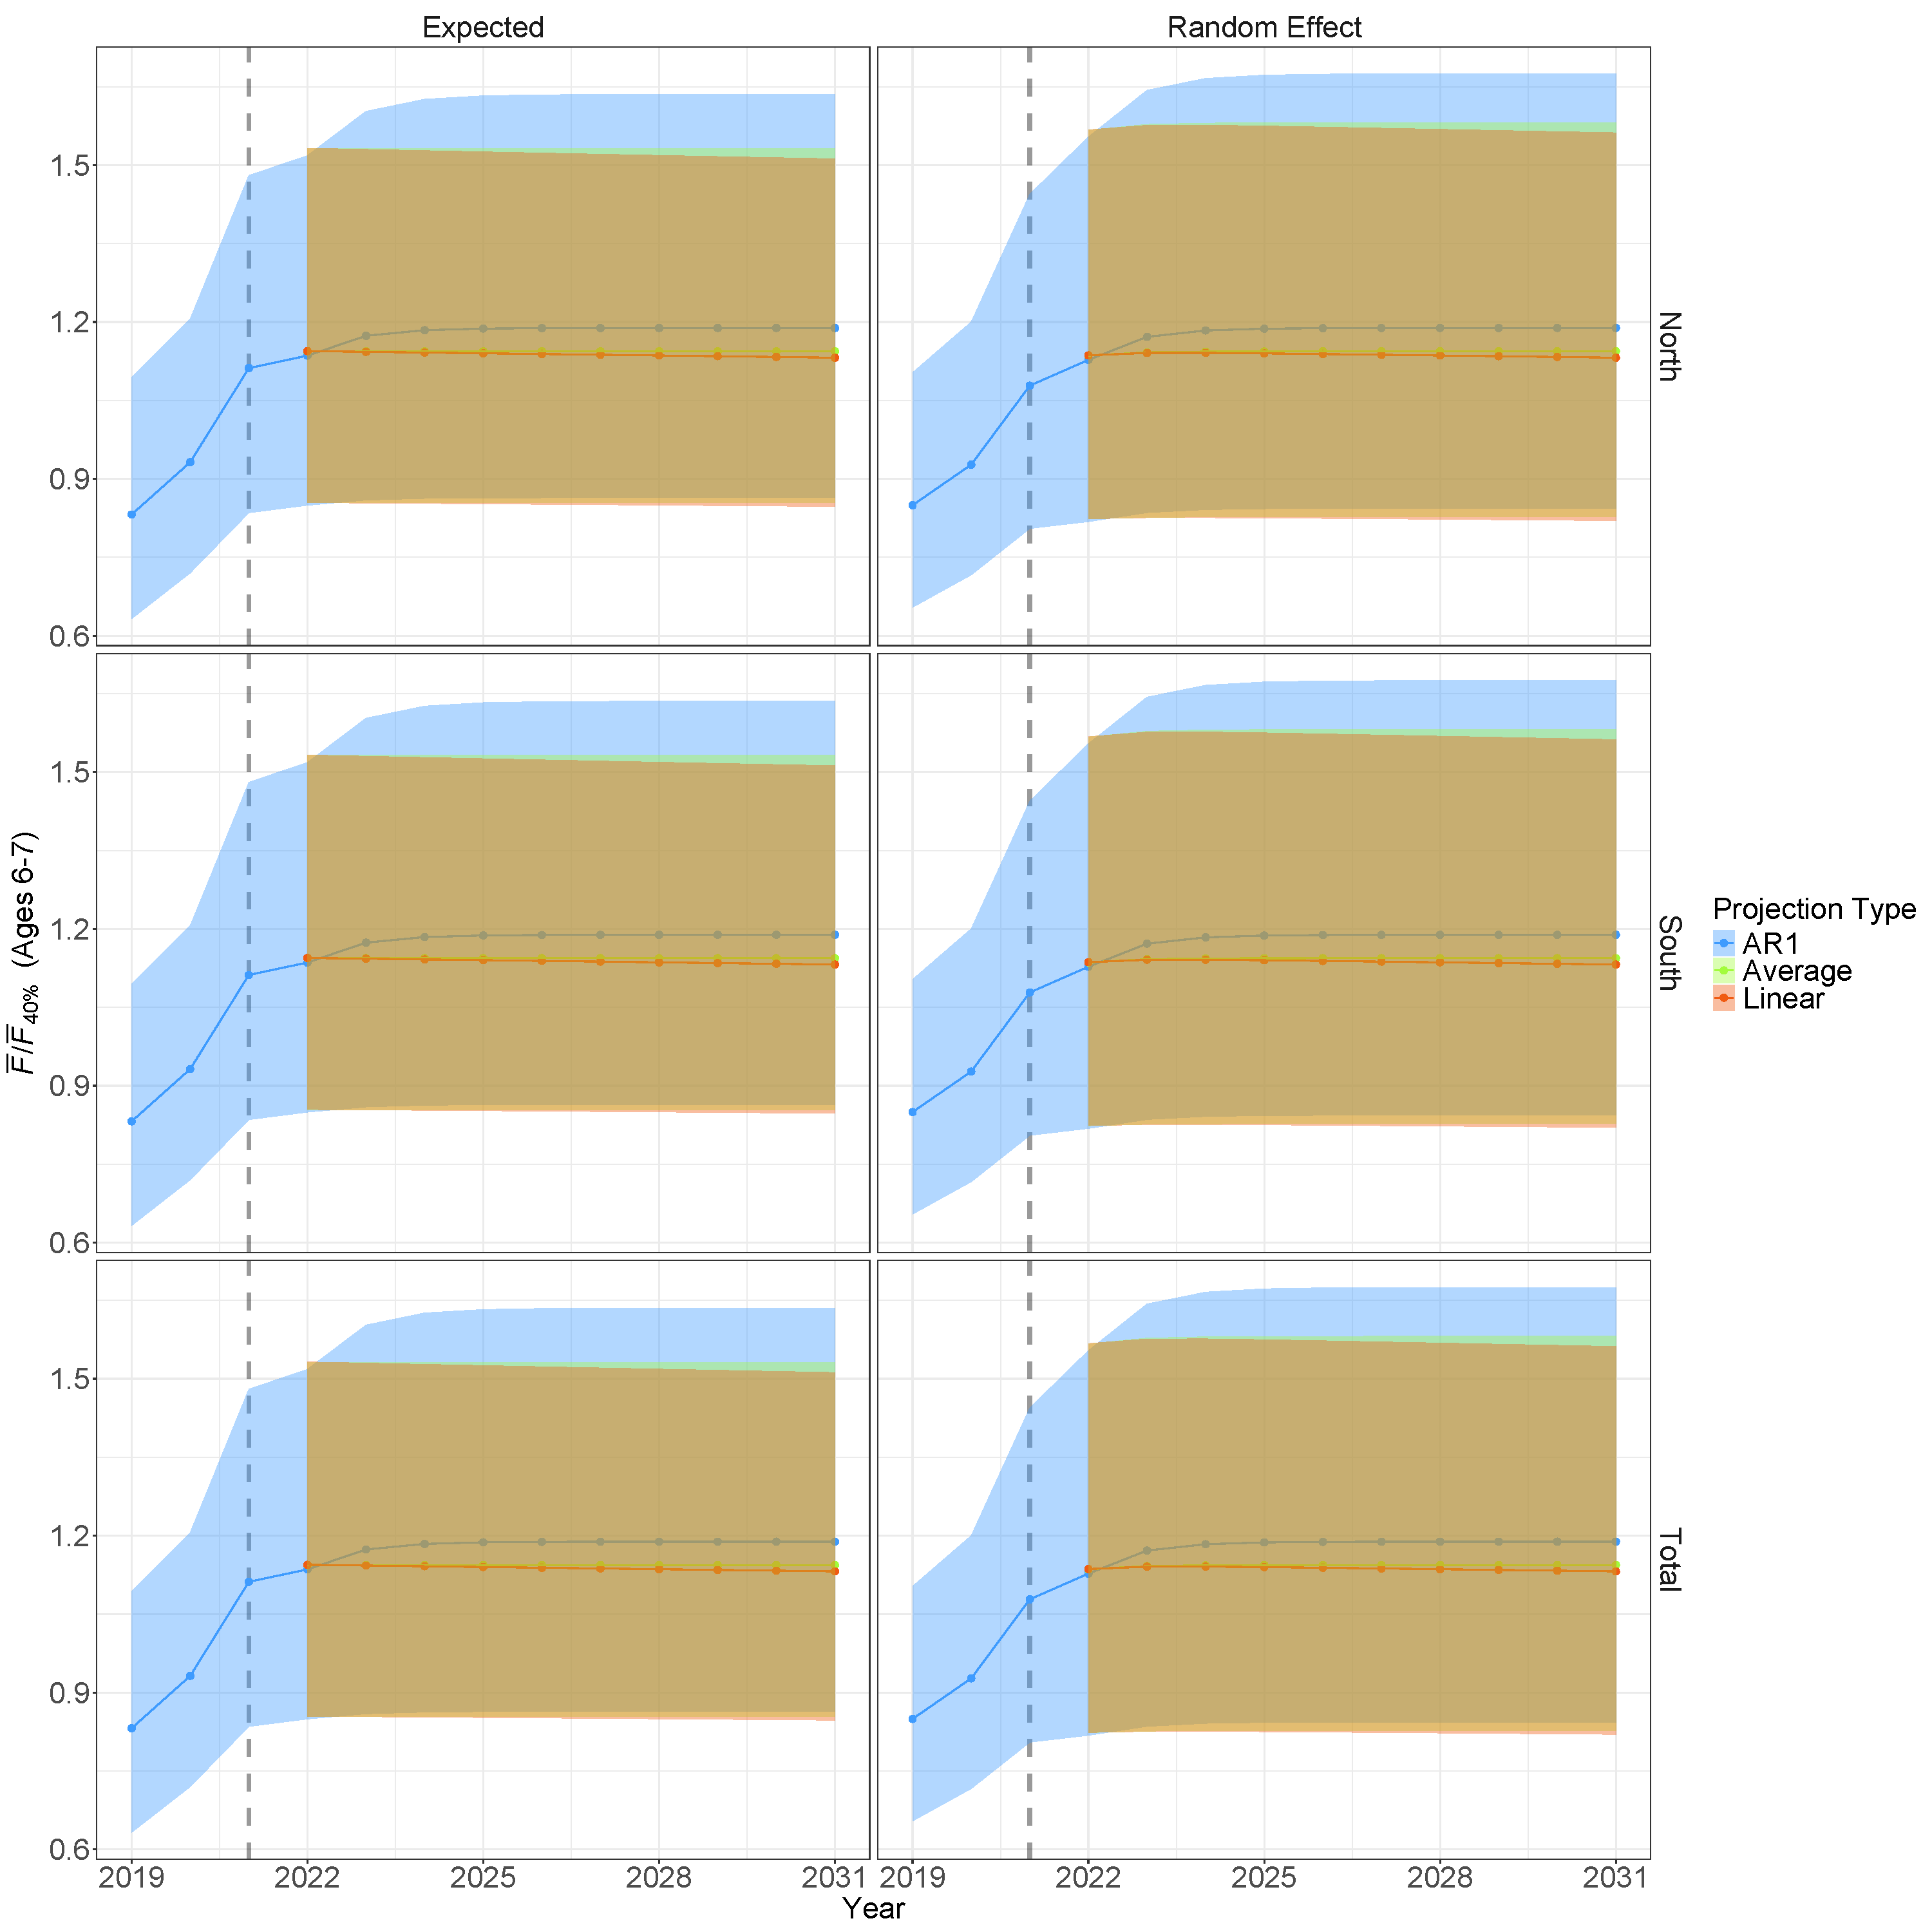
\includegraphics[height=0.95\textheight]{proj_F_status_results} 

}

\caption{Annual estimates of ratios of fishing mortality to $F_{40\%}$ by region and in total. Estimates in years beyond 2021 are from projecting model $M_1$ under alternative assumptions for bottom temperature anomalies in the northern region. Vertical dotted \DIFdelbeginFL \DIFdelFL{line is }\DIFdelendFL \DIFaddbeginFL \DIFaddFL{lines indicate }\DIFaddendFL the last year of data and polygons represent 95\% confidence intervals.}\label{fig:F-status-proj}
\end{figure}
\begin{figure}

{\centering 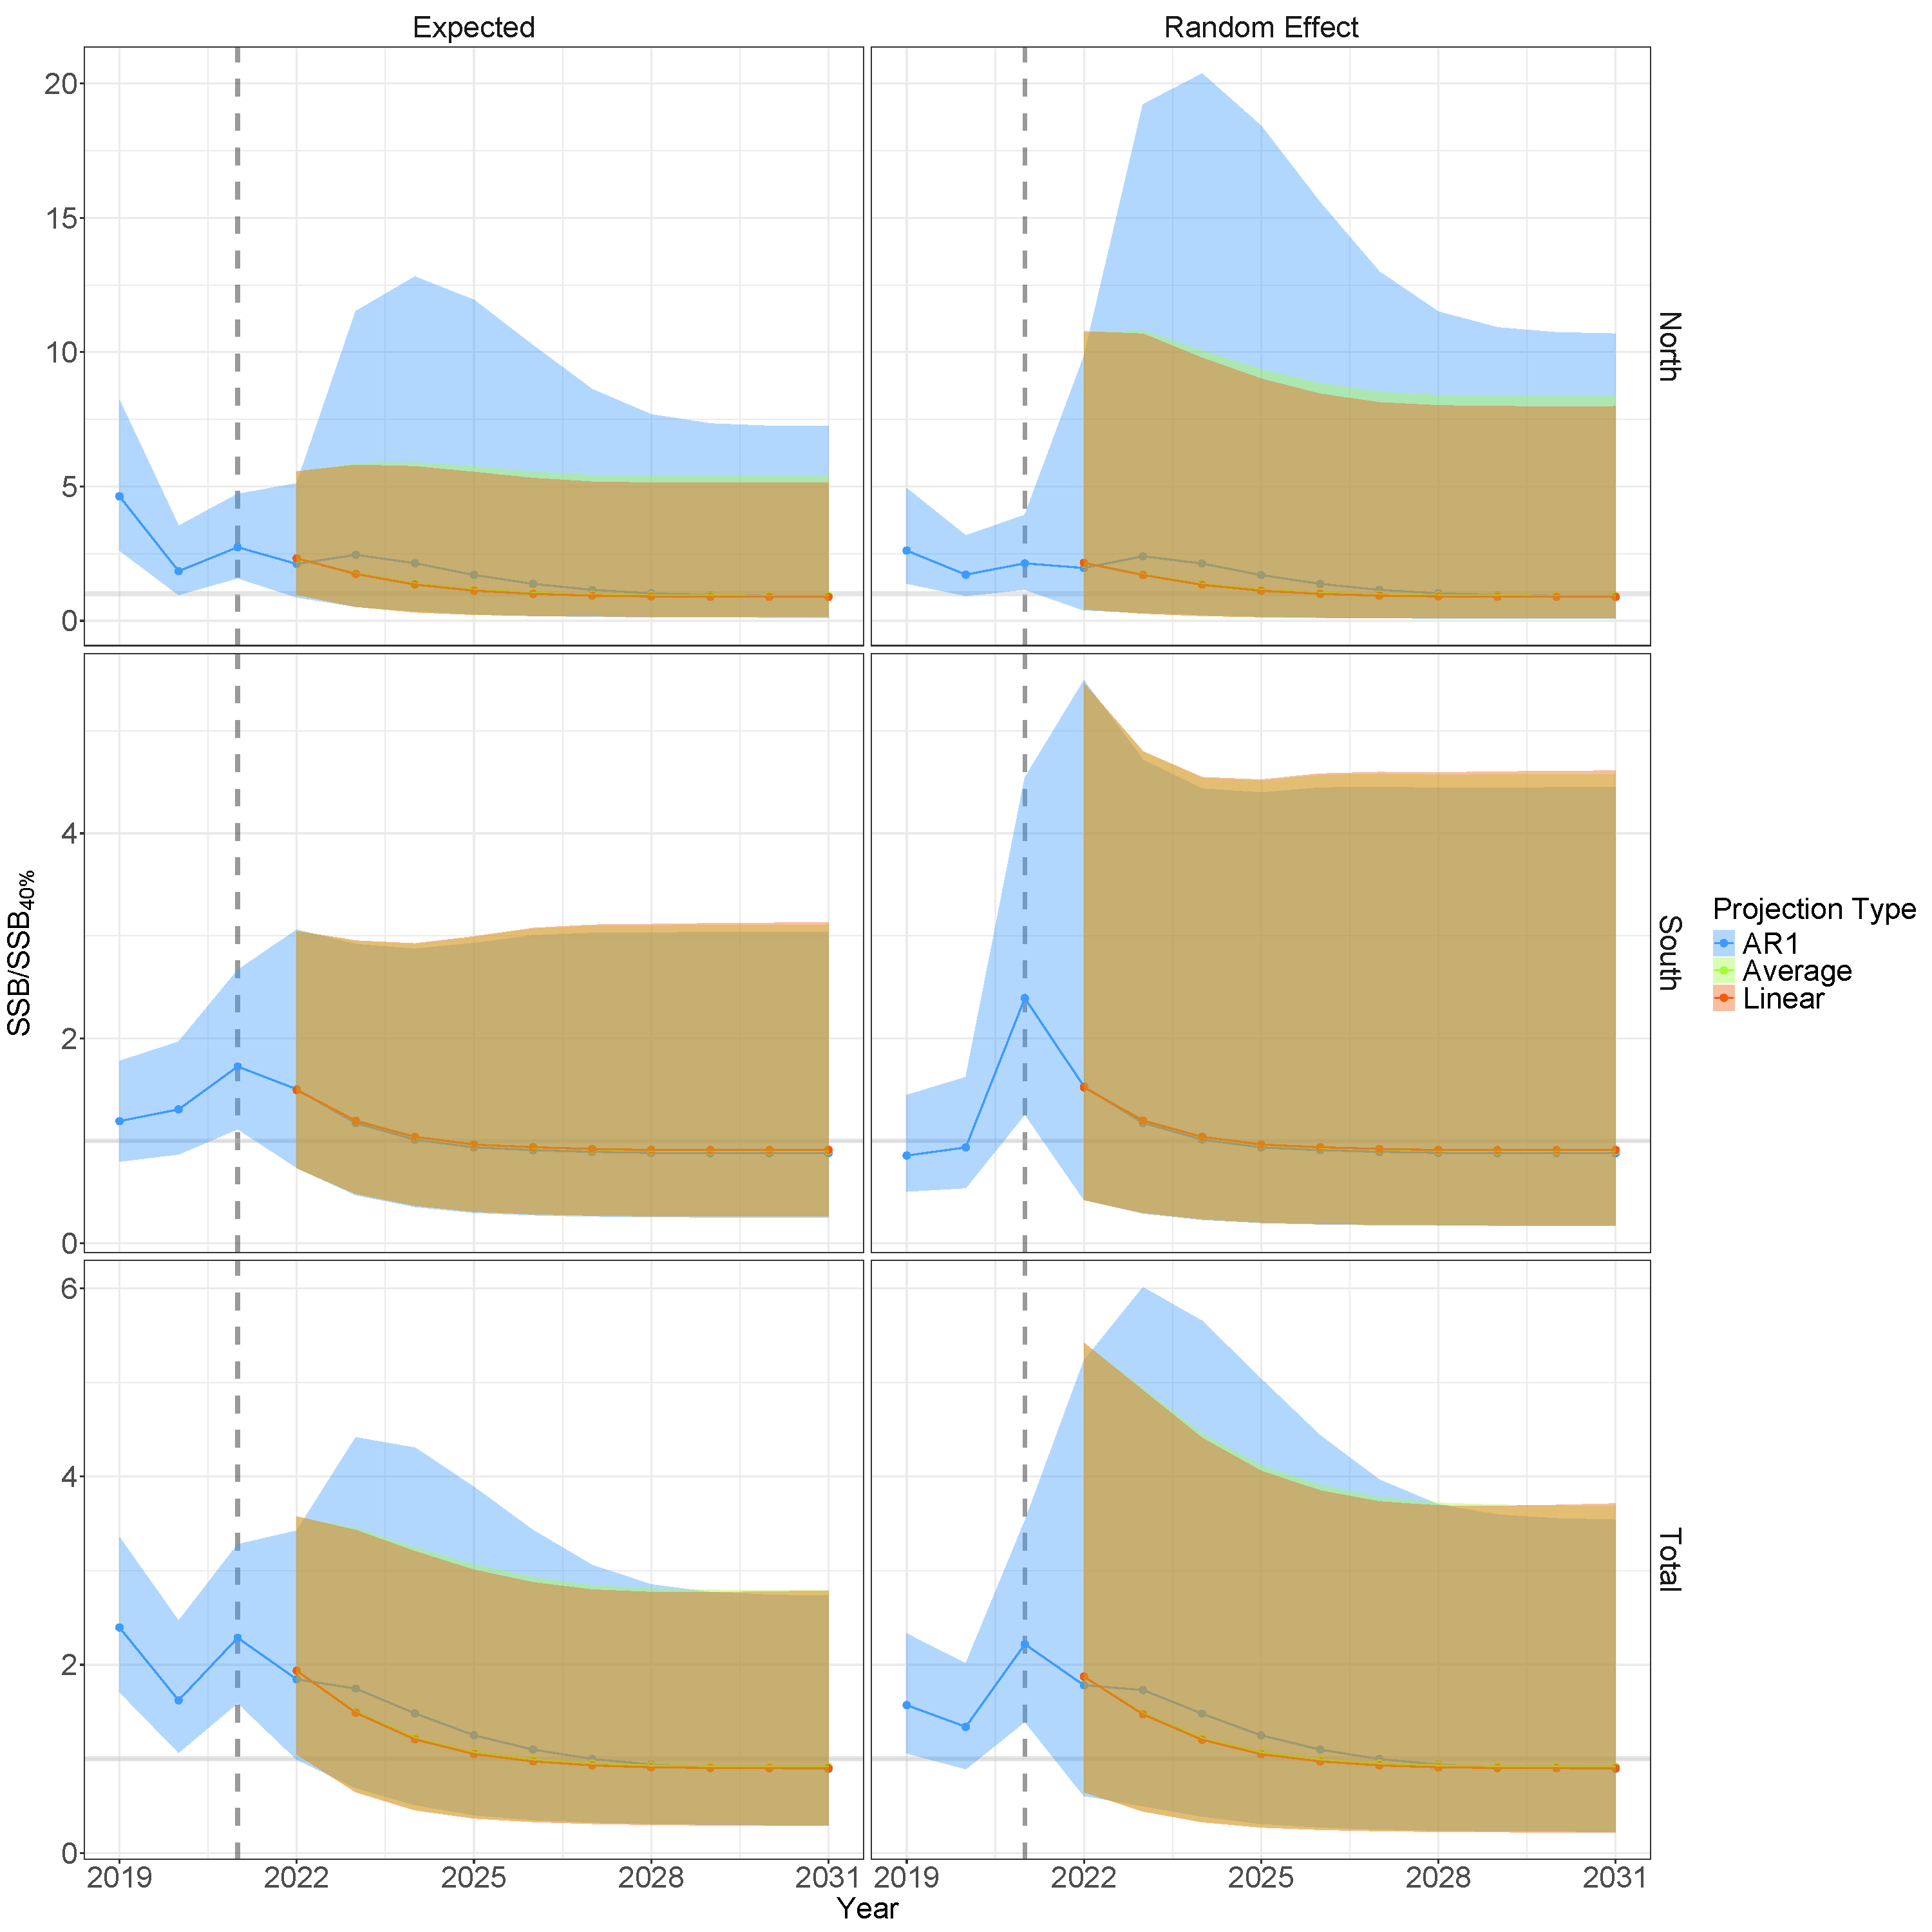
\includegraphics[height=0.95\textheight]{proj_SSB_status_results} 

}

\caption{Annual estimates of ratios of SSB to SSB$_{40\%}$ by region and in total. Estimates in years beyond 2021 are from projecting model $M_1$ under alternative assumptions for bottom temperature anomalies in the northern region. Vertical dotted \DIFdelbeginFL \DIFdelFL{line is }\DIFdelendFL \DIFaddbeginFL \DIFaddFL{lines indicate }\DIFaddendFL the last year of data and polygons represent 95\% confidence intervals.}\label{fig:SSB-status-proj}
\end{figure}

\begin{figure}

{\centering 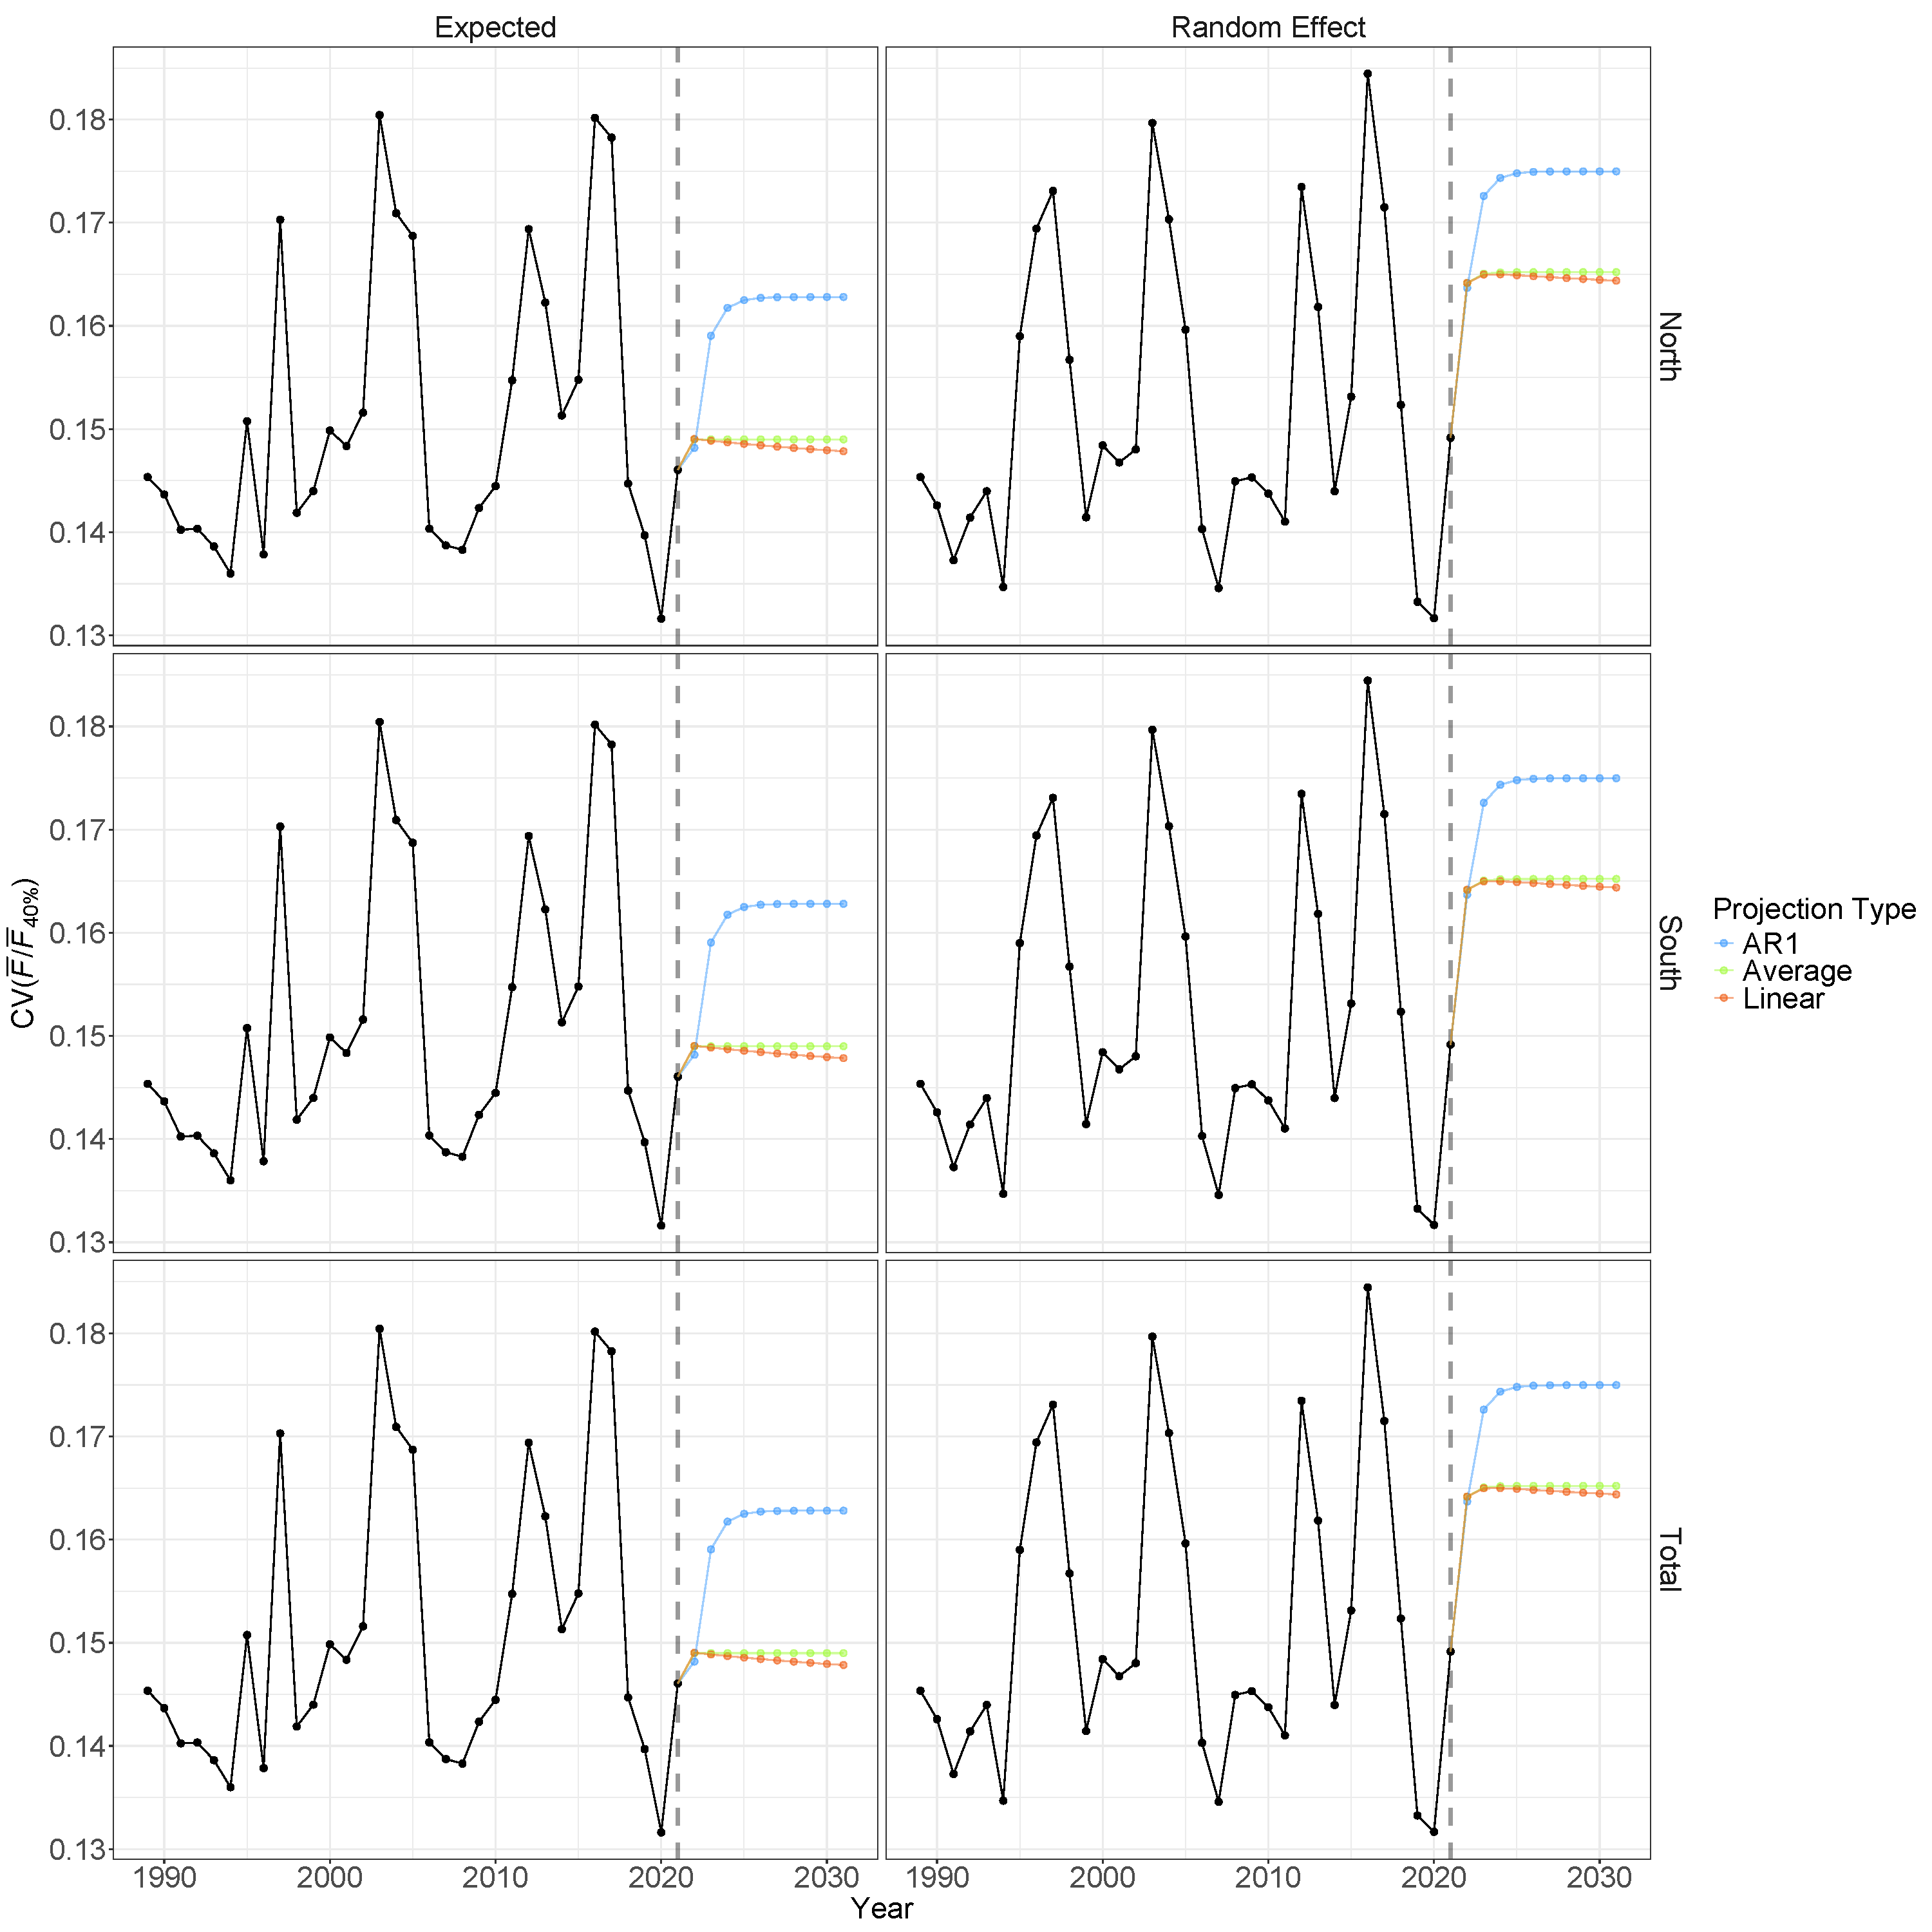
\includegraphics[height=0.95\textheight]{proj_F_status_CV} 

}

\caption{Coefficients of variation for annual ratios of average fishing mortality and equilibrium $\bar{F}_{40\%}$ at ages 6 and 7 where the latter is a function of annual expected recruitment or recruitment random effects and annual inputs to $\upphi(\widetilde{F})$ calculations. Estimates in years after 2021 are from projecting model $M_1$ under three alternative assumptions for the bottom temperature anomolies. \DIFaddbeginFL \DIFaddFL{Vertical dotted lines indicate the last year of data.}\DIFaddendFL }\label{fig:annual-F-status-cvs}
\end{figure}

\begin{figure}

{\centering 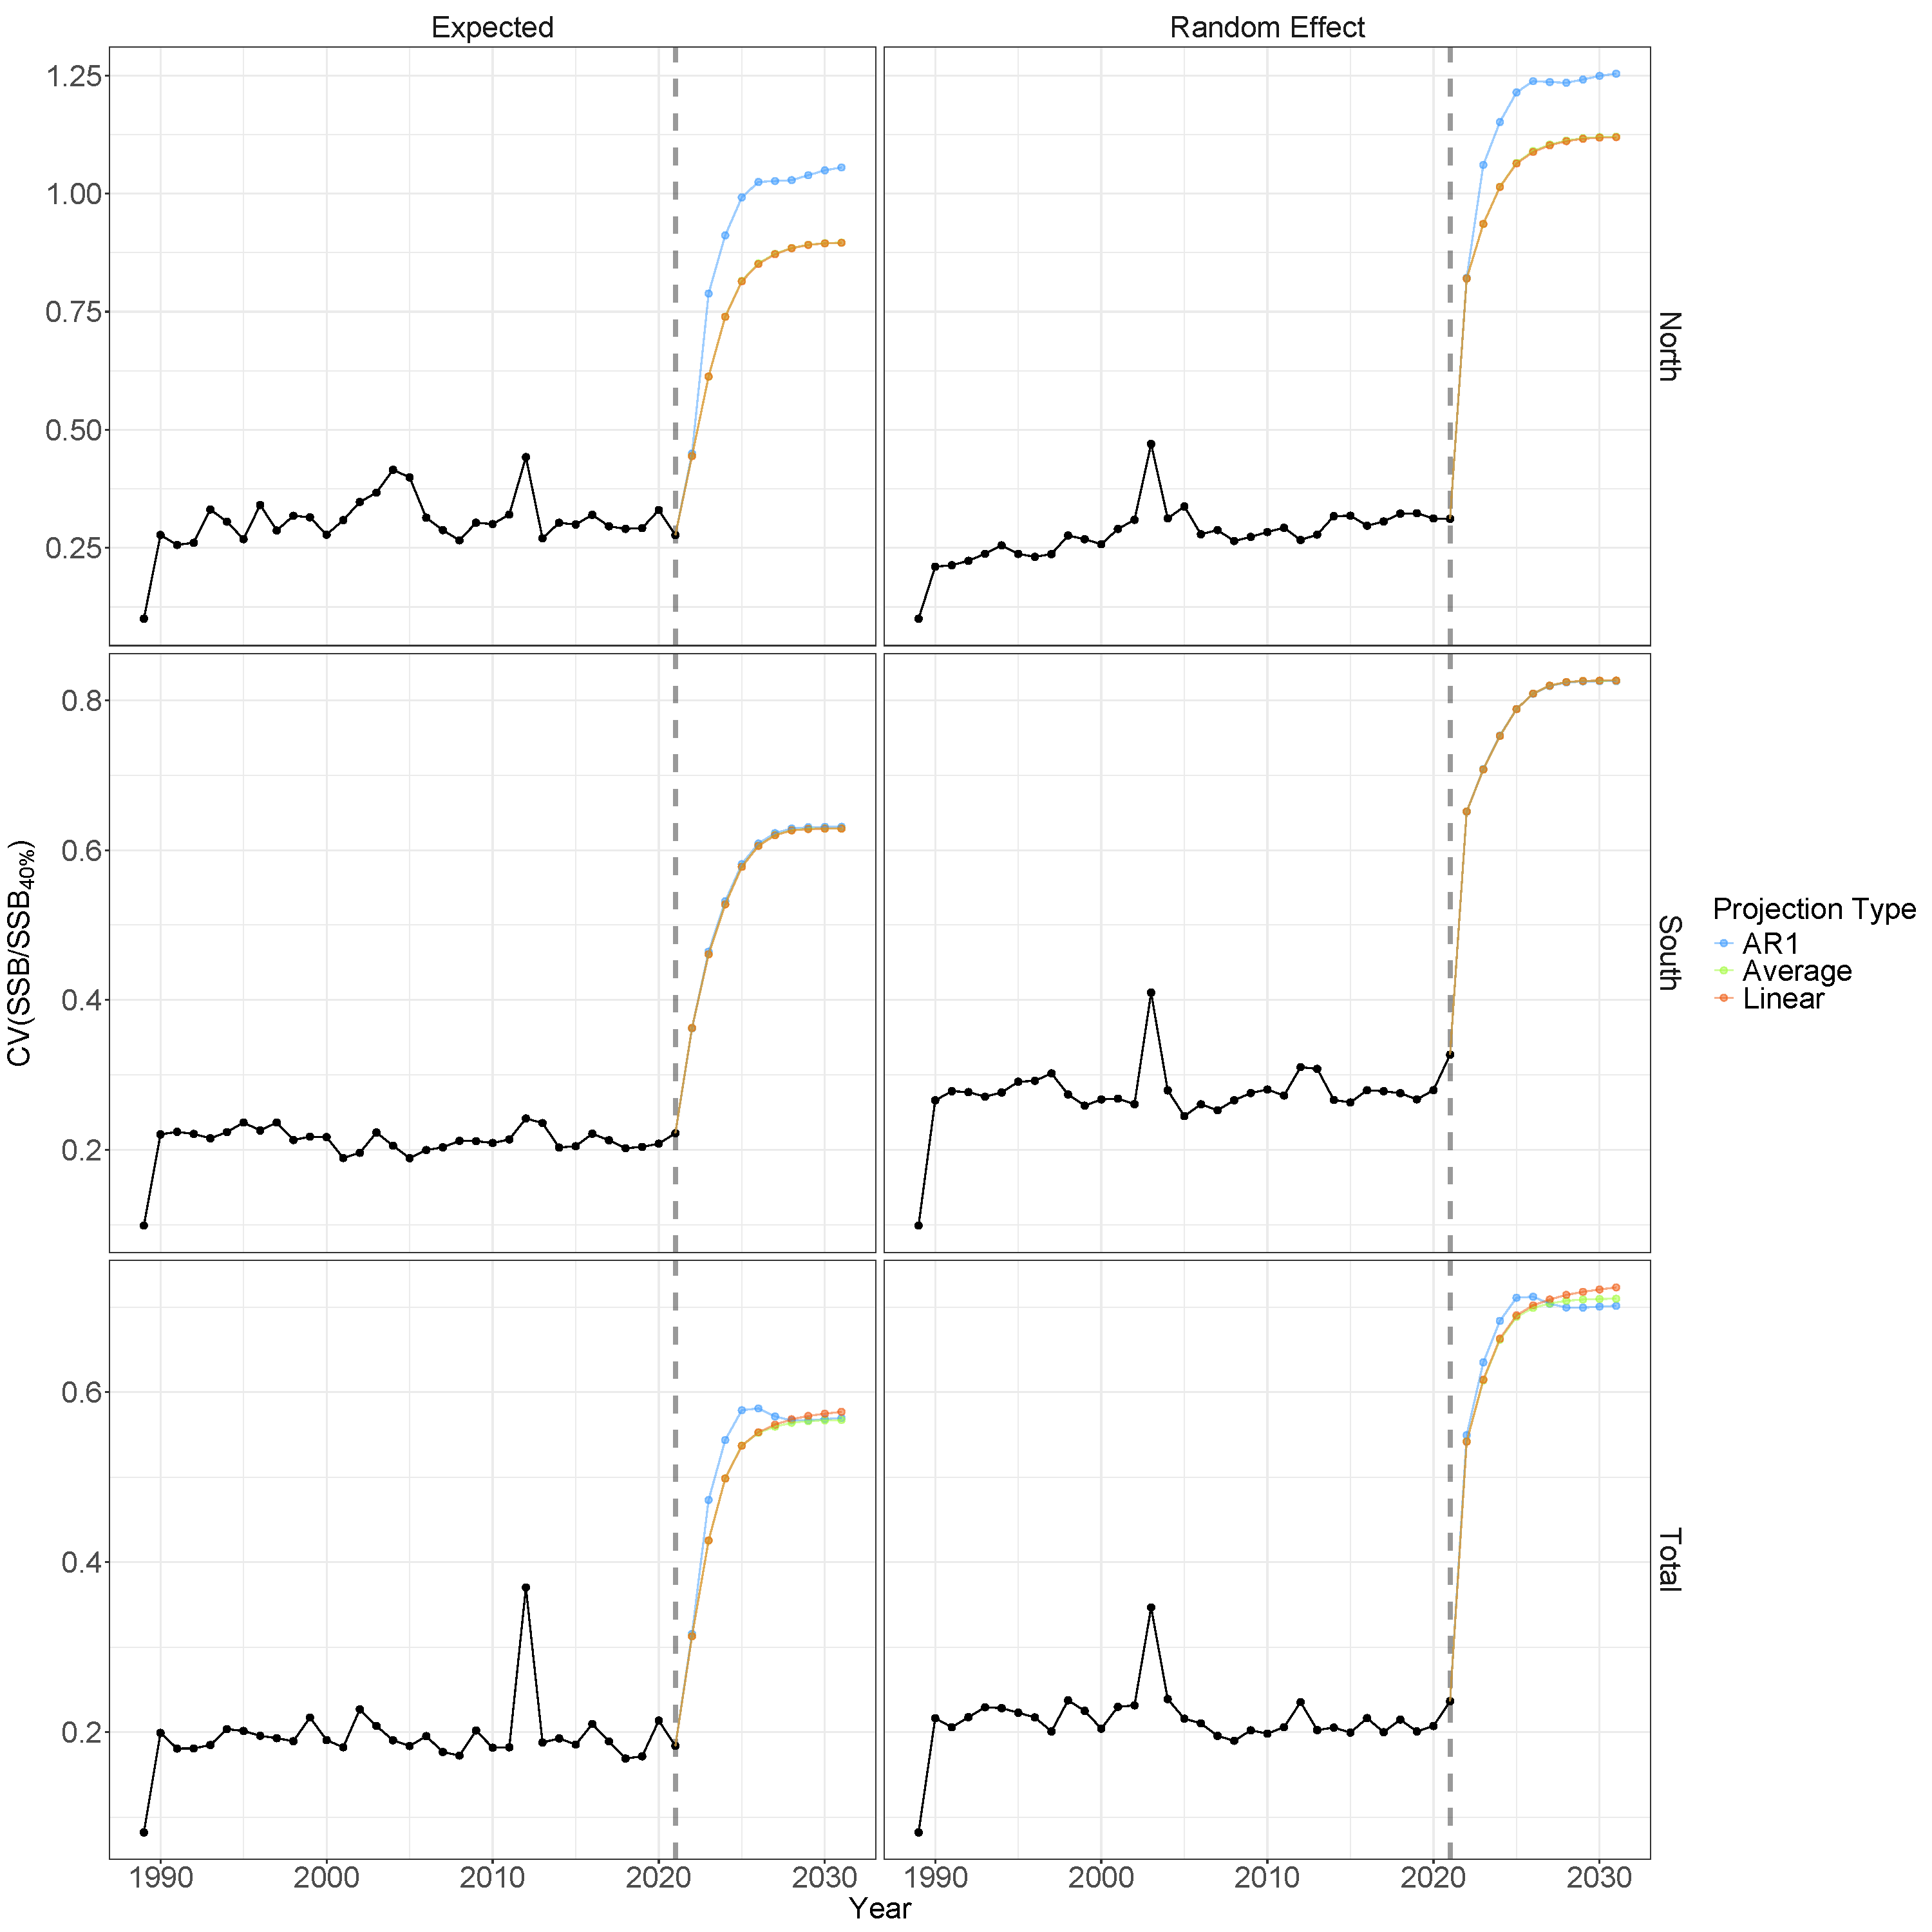
\includegraphics[height=0.95\textheight]{proj_SSB_status_CV} 

}

\caption{Coefficients of variation for annual ratios of SSB and equilibrium SSB$_{40\%}$ where the latter is a function of annual expected recruitment or recruitment random effects and annual inputs to $\upphi(\widetilde{F})$ calculations. Estimates in years after 2021 are from projecting model $M_1$ under three alternative assumptions for the bottom temperature anomolies\DIFaddbeginFL \DIFaddFL{. Vertical dotted lines indicate the last year of data}\DIFaddendFL .}\label{fig:annual-SSB-status-cvs}
\end{figure}

\begin{landscape}

\begin{figure}

{\centering 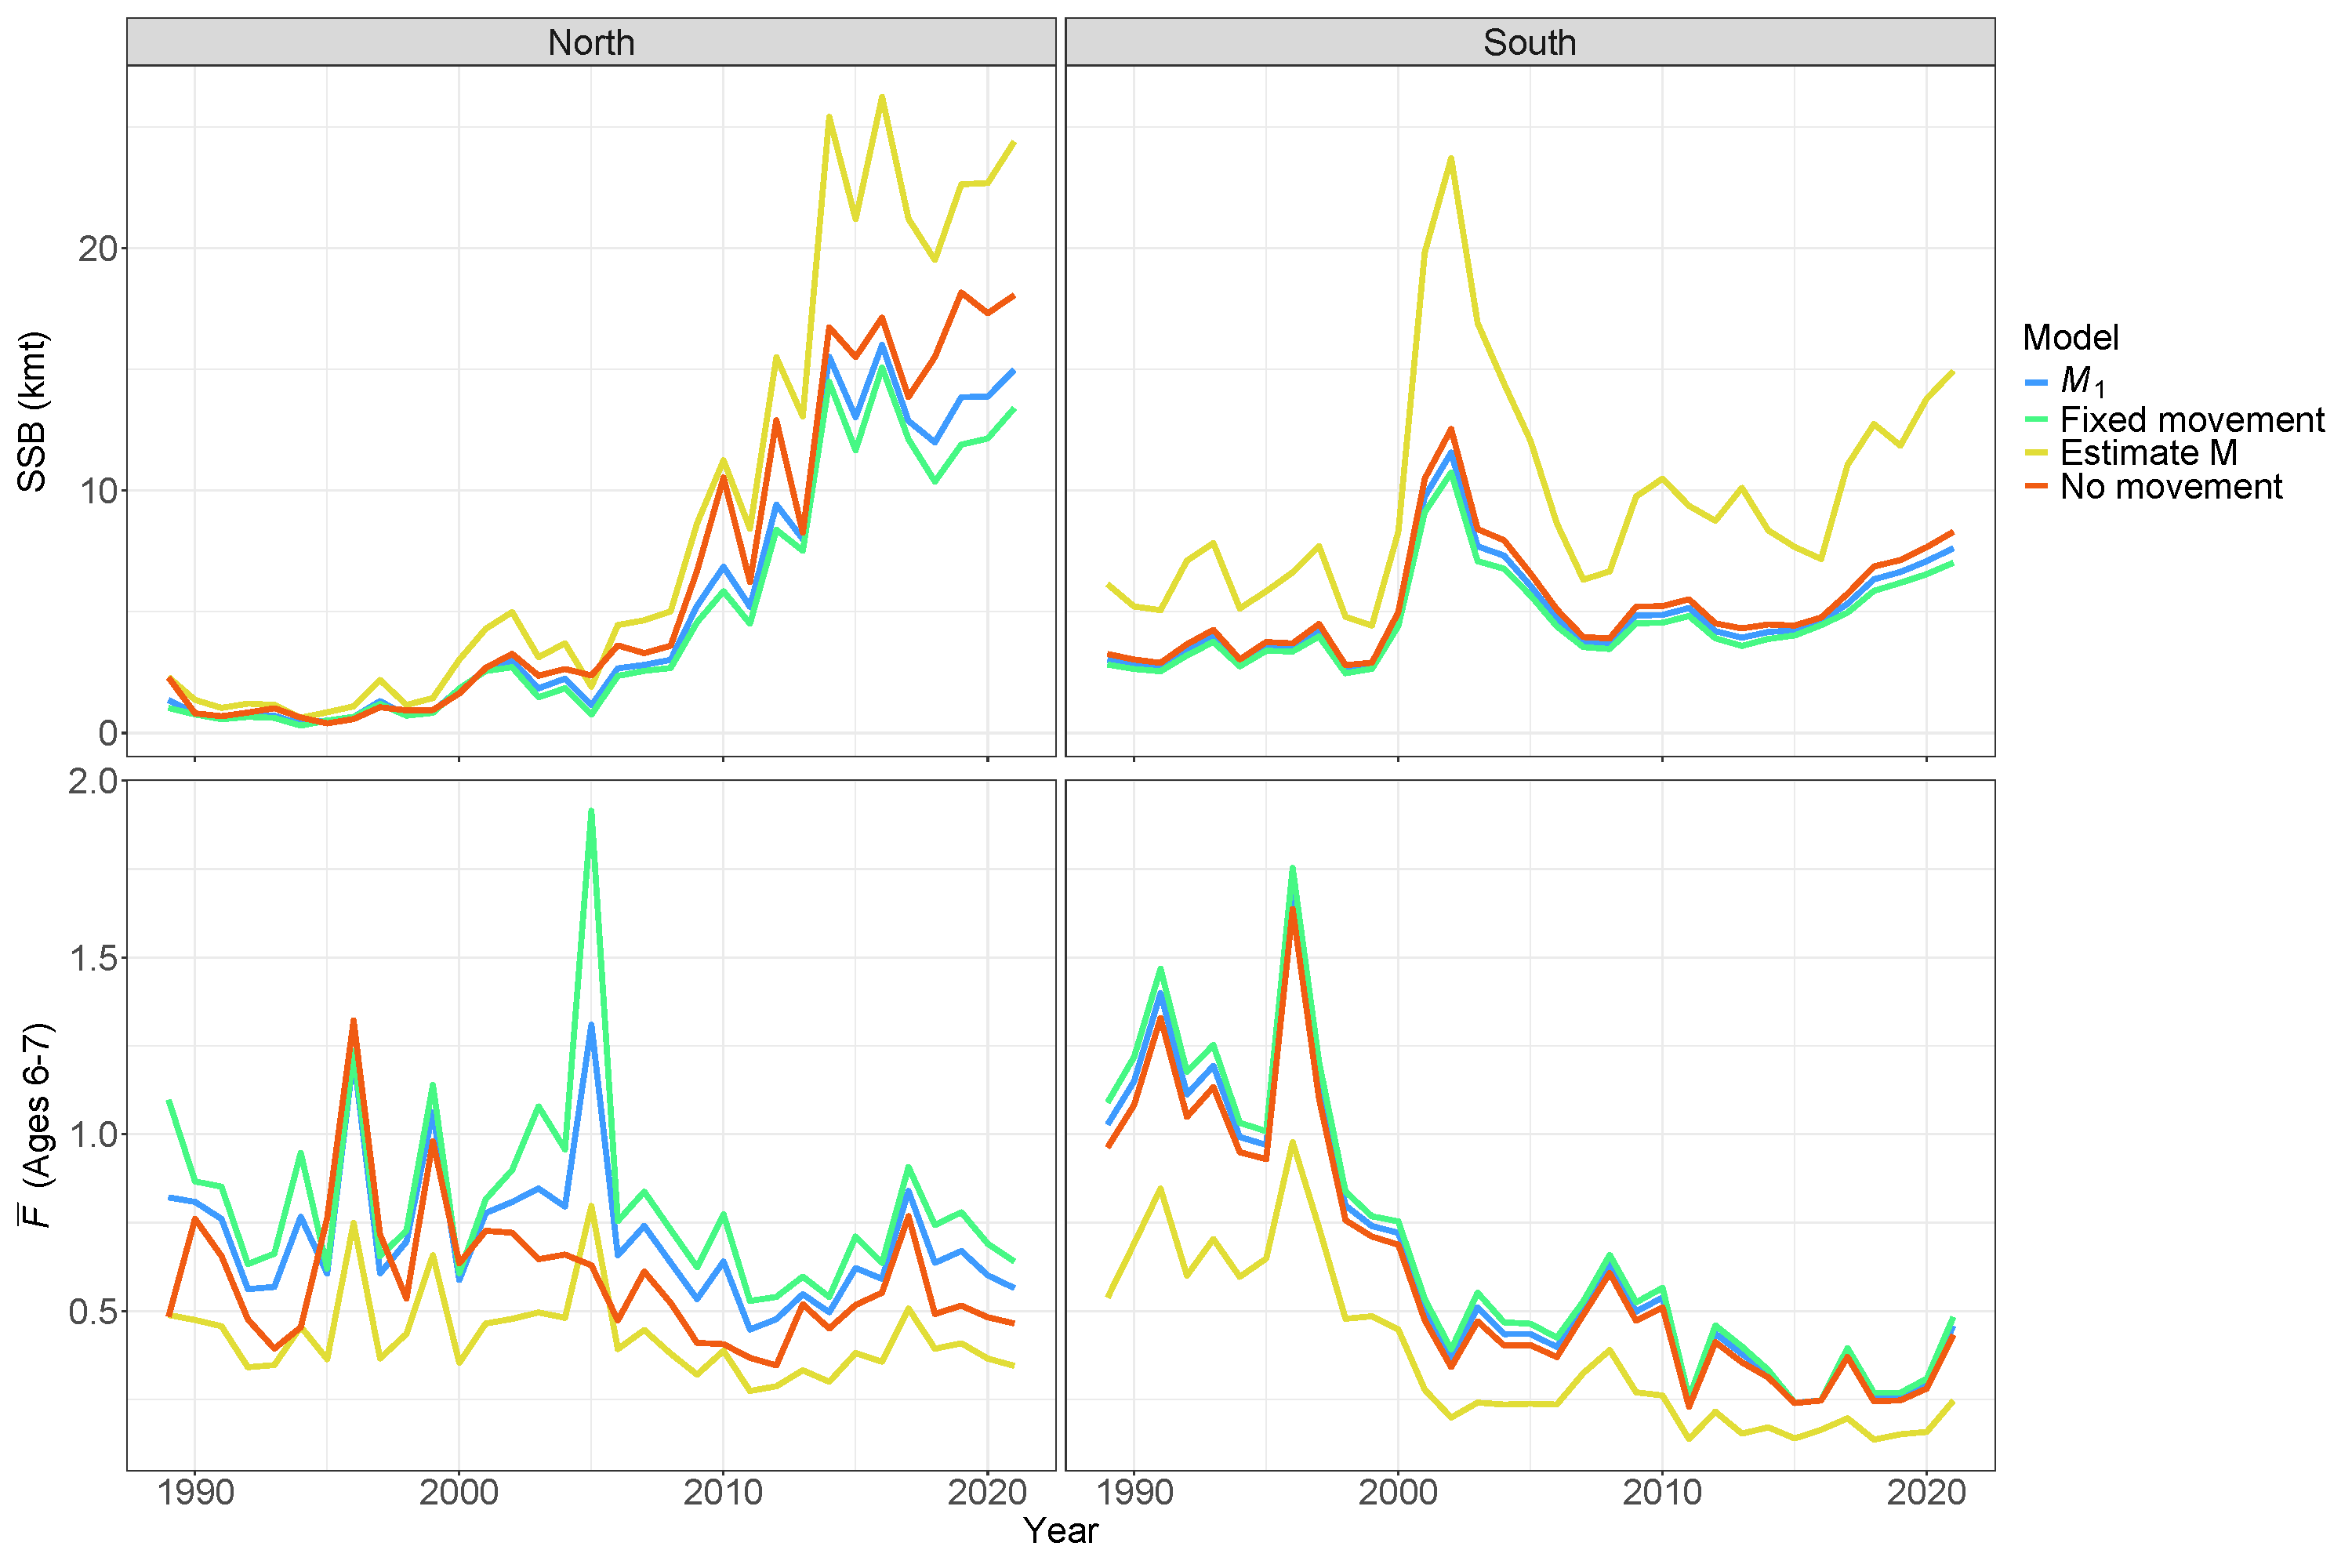
\includegraphics[height=0.95\textheight]{SSB_F_sensitivity_plots} 

}

\caption{Estimates of annual SSB and fishing mortality rates for the best performing model $M_1$ and models that are otherwise the same except where  1) movement rates are fixed at the means for the prior distribution, 2) a constant natural mortality rate is estimated, or 3) there is no movement for either stock component.}\label{fig:sensitivity-plots}
\end{figure}
\end{landscape}

\end{document}
